% Options for packages loaded elsewhere
\PassOptionsToPackage{unicode}{hyperref}
\PassOptionsToPackage{hyphens}{url}
\PassOptionsToPackage{dvipsnames,svgnames,x11names}{xcolor}
%
\documentclass[
  11pt,
  letterpaper,
]{article}

\usepackage{amsmath,amssymb}
\usepackage{setspace}
\usepackage{iftex}
\ifPDFTeX
  \usepackage[T1]{fontenc}
  \usepackage[utf8]{inputenc}
  \usepackage{textcomp} % provide euro and other symbols
\else % if luatex or xetex
  \usepackage{unicode-math}
  \defaultfontfeatures{Scale=MatchLowercase}
  \defaultfontfeatures[\rmfamily]{Ligatures=TeX,Scale=1}
\fi
\usepackage{lmodern}
\ifPDFTeX\else  
    % xetex/luatex font selection
  \setmathfont[]{Libertinus Math}
\fi
% Use upquote if available, for straight quotes in verbatim environments
\IfFileExists{upquote.sty}{\usepackage{upquote}}{}
\IfFileExists{microtype.sty}{% use microtype if available
  \usepackage[]{microtype}
  \UseMicrotypeSet[protrusion]{basicmath} % disable protrusion for tt fonts
}{}
\makeatletter
\@ifundefined{KOMAClassName}{% if non-KOMA class
  \IfFileExists{parskip.sty}{%
    \usepackage{parskip}
  }{% else
    \setlength{\parindent}{0pt}
    \setlength{\parskip}{6pt plus 2pt minus 1pt}}
}{% if KOMA class
  \KOMAoptions{parskip=half}}
\makeatother
\usepackage{xcolor}
\usepackage[top=1in,bottom=1in,left=1in,right=1in,heightrounded]{geometry}
\setlength{\emergencystretch}{3em} % prevent overfull lines
\setcounter{secnumdepth}{-\maxdimen} % remove section numbering
% Make \paragraph and \subparagraph free-standing
\makeatletter
\ifx\paragraph\undefined\else
  \let\oldparagraph\paragraph
  \renewcommand{\paragraph}{
    \@ifstar
      \xxxParagraphStar
      \xxxParagraphNoStar
  }
  \newcommand{\xxxParagraphStar}[1]{\oldparagraph*{#1}\mbox{}}
  \newcommand{\xxxParagraphNoStar}[1]{\oldparagraph{#1}\mbox{}}
\fi
\ifx\subparagraph\undefined\else
  \let\oldsubparagraph\subparagraph
  \renewcommand{\subparagraph}{
    \@ifstar
      \xxxSubParagraphStar
      \xxxSubParagraphNoStar
  }
  \newcommand{\xxxSubParagraphStar}[1]{\oldsubparagraph*{#1}\mbox{}}
  \newcommand{\xxxSubParagraphNoStar}[1]{\oldsubparagraph{#1}\mbox{}}
\fi
\makeatother


\providecommand{\tightlist}{%
  \setlength{\itemsep}{0pt}\setlength{\parskip}{0pt}}\usepackage{longtable,booktabs,array}
\usepackage{calc} % for calculating minipage widths
% Correct order of tables after \paragraph or \subparagraph
\usepackage{etoolbox}
\makeatletter
\patchcmd\longtable{\par}{\if@noskipsec\mbox{}\fi\par}{}{}
\makeatother
% Allow footnotes in longtable head/foot
\IfFileExists{footnotehyper.sty}{\usepackage{footnotehyper}}{\usepackage{footnote}}
\makesavenoteenv{longtable}
\usepackage{graphicx}
\makeatletter
\newsavebox\pandoc@box
\newcommand*\pandocbounded[1]{% scales image to fit in text height/width
  \sbox\pandoc@box{#1}%
  \Gscale@div\@tempa{\textheight}{\dimexpr\ht\pandoc@box+\dp\pandoc@box\relax}%
  \Gscale@div\@tempb{\linewidth}{\wd\pandoc@box}%
  \ifdim\@tempb\p@<\@tempa\p@\let\@tempa\@tempb\fi% select the smaller of both
  \ifdim\@tempa\p@<\p@\scalebox{\@tempa}{\usebox\pandoc@box}%
  \else\usebox{\pandoc@box}%
  \fi%
}
% Set default figure placement to htbp
\def\fps@figure{htbp}
\makeatother
% definitions for citeproc citations
\NewDocumentCommand\citeproctext{}{}
\NewDocumentCommand\citeproc{mm}{%
  \begingroup\def\citeproctext{#2}\cite{#1}\endgroup}
\makeatletter
 % allow citations to break across lines
 \let\@cite@ofmt\@firstofone
 % avoid brackets around text for \cite:
 \def\@biblabel#1{}
 \def\@cite#1#2{{#1\if@tempswa , #2\fi}}
\makeatother
\newlength{\cslhangindent}
\setlength{\cslhangindent}{1.5em}
\newlength{\csllabelwidth}
\setlength{\csllabelwidth}{3em}
\newenvironment{CSLReferences}[2] % #1 hanging-indent, #2 entry-spacing
 {\begin{list}{}{%
  \setlength{\itemindent}{0pt}
  \setlength{\leftmargin}{0pt}
  \setlength{\parsep}{0pt}
  % turn on hanging indent if param 1 is 1
  \ifodd #1
   \setlength{\leftmargin}{\cslhangindent}
   \setlength{\itemindent}{-1\cslhangindent}
  \fi
  % set entry spacing
  \setlength{\itemsep}{#2\baselineskip}}}
 {\end{list}}
\usepackage{calc}
\newcommand{\CSLBlock}[1]{\hfill\break\parbox[t]{\linewidth}{\strut\ignorespaces#1\strut}}
\newcommand{\CSLLeftMargin}[1]{\parbox[t]{\csllabelwidth}{\strut#1\strut}}
\newcommand{\CSLRightInline}[1]{\parbox[t]{\linewidth - \csllabelwidth}{\strut#1\strut}}
\newcommand{\CSLIndent}[1]{\hspace{\cslhangindent}#1}

\usepackage{booktabs}
\usepackage{caption}
\usepackage{longtable}
\usepackage{colortbl}
\usepackage{array}
\usepackage{anyfontsize}
\usepackage{multirow}
\usepackage{mathtools}
\everydisplay\expandafter{\the\everydisplay\small}
\usepackage{float}
\floatplacement{figure}{H}
\floatplacement{table}{H}
\usepackage{setspace}
\pagenumbering{arabic}
\usepackage{titlesec}
\titleformat{\section}{\fontsize{12}{14}\bfseries}{\thesection}{1em}{}
\titleformat{\subsection}{\fontsize{11}{14}\bfseries}{\thesubsection}{1em}{}
\titleformat{\subsubsection}{\fontsize{11}{14}\bfseries}{\thesubsubsection}{1em}{}
\titleformat{\paragraph}{\fontsize{12}{14}\bfseries}{}{0em}{} 
\makeatletter
\@ifpackageloaded{tcolorbox}{}{\usepackage[skins,breakable]{tcolorbox}}
\@ifpackageloaded{fontawesome5}{}{\usepackage{fontawesome5}}
\definecolor{quarto-callout-color}{HTML}{909090}
\definecolor{quarto-callout-note-color}{HTML}{0758E5}
\definecolor{quarto-callout-important-color}{HTML}{CC1914}
\definecolor{quarto-callout-warning-color}{HTML}{EB9113}
\definecolor{quarto-callout-tip-color}{HTML}{00A047}
\definecolor{quarto-callout-caution-color}{HTML}{FC5300}
\definecolor{quarto-callout-color-frame}{HTML}{acacac}
\definecolor{quarto-callout-note-color-frame}{HTML}{4582ec}
\definecolor{quarto-callout-important-color-frame}{HTML}{d9534f}
\definecolor{quarto-callout-warning-color-frame}{HTML}{f0ad4e}
\definecolor{quarto-callout-tip-color-frame}{HTML}{02b875}
\definecolor{quarto-callout-caution-color-frame}{HTML}{fd7e14}
\makeatother
\makeatletter
\@ifpackageloaded{caption}{}{\usepackage{caption}}
\AtBeginDocument{%
\ifdefined\contentsname
  \renewcommand*\contentsname{Table of contents}
\else
  \newcommand\contentsname{Table of contents}
\fi
\ifdefined\listfigurename
  \renewcommand*\listfigurename{List of Figures}
\else
  \newcommand\listfigurename{List of Figures}
\fi
\ifdefined\listtablename
  \renewcommand*\listtablename{List of Tables}
\else
  \newcommand\listtablename{List of Tables}
\fi
\ifdefined\figurename
  \renewcommand*\figurename{Figure}
\else
  \newcommand\figurename{Figure}
\fi
\ifdefined\tablename
  \renewcommand*\tablename{Table}
\else
  \newcommand\tablename{Table}
\fi
}
\@ifpackageloaded{float}{}{\usepackage{float}}
\floatstyle{ruled}
\@ifundefined{c@chapter}{\newfloat{codelisting}{h}{lop}}{\newfloat{codelisting}{h}{lop}[chapter]}
\floatname{codelisting}{Listing}
\newcommand*\listoflistings{\listof{codelisting}{List of Listings}}
\makeatother
\makeatletter
\makeatother
\makeatletter
\@ifpackageloaded{caption}{}{\usepackage{caption}}
\@ifpackageloaded{subcaption}{}{\usepackage{subcaption}}
\makeatother
\makeatletter
\@ifpackageloaded{sidenotes}{}{\usepackage{sidenotes}}
\@ifpackageloaded{marginnote}{}{\usepackage{marginnote}}
\makeatother
\makeatletter
\@ifpackageloaded{fontawesome5}{}{\usepackage{fontawesome5}}
\makeatother

\usepackage{bookmark}

\IfFileExists{xurl.sty}{\usepackage{xurl}}{} % add URL line breaks if available
\urlstyle{same} % disable monospaced font for URLs
\hypersetup{
  colorlinks=true,
  linkcolor={Black},
  filecolor={Maroon},
  citecolor={Black},
  urlcolor={Black},
  pdfcreator={LaTeX via pandoc}}


\author{}
\date{2024-10-12}

\begin{document}


\setstretch{1.5}
\begin{centering}

{THE ROLE OF VARIABILITY IN LEARNING GENERALIZATION: A COMPUTATIONAL MODELING APPROACH}

 
\vspace{5\baselineskip}

{Thomas E. Gorman}

\vspace{10.5cm}



Submitted to the faculty of the University Graduate School \\
in partial fulfillment of the requirements \\
for the degree \\
Doctor of Philosophy \\
in the Cognitive Science Program and \\
Department of Psychological and Brain Sciences, \\
Indiana University \\
October 2024


\vspace{6cm}

\pagenumbering{gobble}
\end{centering}

\newpage
\pagenumbering{roman}
\setcounter{page}{2}
\begin{center}

Accepted by the Graduate Faculty, Indiana University, in partial fulfillment of the
requirements for the degree of Doctor of Philosophy.
\end{center}
\vspace{1cm}

\hfill\break
Doctoral Committee \vspace{1cm}

\begin{flushright}
\underline{\hspace{5cm}} \\
Robert L. Goldstone, Ph.D.
\vspace{2cm}

\underline{\hspace{5cm}} \\
Robert M. Nosofsky, Ph.D.
\vspace{2cm}

\underline{\hspace{5cm}} \\
Peter M. Todd, Ph.D.
\vspace{2cm}

\underline{\hspace{5cm}} \\
Michael N. Jones, Ph.D.
\end{flushright}

\hfill\break
May 28th, 2024

\newpage

\begin{centering}

\vspace*{6.5cm}

@2024 \\
\vspace{1cm} 

Thomas E. Gorman
\vspace{.2cm}

\vspace{5cm}

\end{centering}

\newpage

\begin{centering}

\textbf{Acknowledgements}

\end{centering}

My dissertation would not have been possible without the support and
guidance of numerous individuals who have shaped my academic and
personal growth.

First, I am deeply grateful to my advisor, Rob Goldstone, for his nearly
limitless patience, clear thinking, and unwavering guidance. His ability
to effortlessly demonstrate the power of so many tools has been
awe-inspiring, and I am forever thankful for his mentorship. I also
extend my heartfelt thanks to Dr.~Rob Nosofsky for his sharp questions
and encouragement of model-based thinking, and to Dr.~Peter Todd for
being a constant source of encouragement.

My foundation in psychological science was laid at the University of
Wisconsin-Madison. I am indebted to Dr.~Shawn Green, who took a chance
on me despite my mediocre grades and lack of experience, introducing me
to the world of psychological research. Special thanks to Aaron Cochrane
for answering my countless questions, introducing me to R, and advanced
data analysis techniques.

I am grateful for the camaraderie and intellectual stimulation provided
by my friends at Indiana University, particularly those in the Geolab
and Psychology department. Johnathan Avery, Eleanor Schille-Hudson, Mahi
Luthra, Dan Levitas, Sam Nordli, Brad Rogers, Marina Dubova, Eeshan
Hasan, and many others have been integral to my graduate school
experience. A special mention goes to Jack Avery for introducing me to
rock climbing and engaging in fun conversations that often led to
unexpected ideas.

The teachers at Pardeeville High School played an essential role in
nurturing my curiosity and establishing the educational foundation that
shaped my early learning. The professors at UW-Madison and Indiana
University further cultivated that curiosity, profoundly influencing my
academic development.

I would also like to extend my heartfelt thanks to my family. My
parents, Mary and Jim Gorman, have always been a source of love and
unwavering belief in my abilities. My brother, Joseph, played a pivotal
role in helping me through the final stages of my dissertation by
providing a supportive environment and the encouragement I needed. Their
collective support has made this journey not only possible but
meaningful, and I will always be deeply grateful for it.

\newpage

\begin{centering}

{Thomas E. Gorman}

{THE ROLE OF VARIABILITY IN LEARNING GENERALIZATION: A COMPUTATIONAL MODELING APPROACH}

\end{centering}

The impact of training variability on generalization has been a
long-standing topic in the study of human learning, with conflicting
evidence about its potential benefits. This dissertation addresses these
ambiguities by examining the effects of varied versus constant training
in visuomotor skill learning through a combination of experimental and
computational modeling approaches. Across two projects, we
systematically compare varied training (multiple items) to constant
training (single item) in a projectile-throwing task. Empirical findings
reveal both positive and negative impacts of variability, highlighting
the complex interplay between training conditions and generalization
performance. To provide a theoretical account of these findings, this
dissertation employs both instance-based and connectionist computational
modeling approaches. The instance-based modeling approach introduced in
project 1 provides a theoretically justifiable method of
quantifying/controlling for similarity between training and testing
conditions, while also demonstrating that varied training may induce
broader generalization in the similarity function relating training and
test items. In project 2, the Extrapolation-Association Model (EXAM)
provided the best account of the testing data across all experiments,
capturing the constant groups' ability to extrapolate to novel regions
despite limited training experience, while also revealing potential
detriments of varied training for simple extrapolation tasks. These
results challenge simplistic notions about the universality of
variability benefits in training and emphasize the need for tailored
approaches that consider both the structure of the task environment and
the prior knowledge of the learners.

\newpage

\newpage{}

\tableofcontents
\newpage

\clearpage
\pagenumbering{arabic}

\newpage{}

\section{Introduction}\label{introduction}

\subsection{Varied Training and
Generalization}\label{varied-training-and-generalization}

Varied training has been shown to influence learning in a wide array of
different tasks and domains, including categorization
(\citeproc{ref-hahnEffectsCategoryDiversity2005}{Hahn et al., 2005};
\citeproc{ref-maddoxStimulusRangeDiscontinuity2011}{Maddox \& Filoteo,
2011};
\citeproc{ref-morgensternOneshotCategorizationNovel2019}{Morgenstern et
al., 2019}; \citeproc{ref-nosofskyModelguidedSearchOptimal2019}{Nosofsky
et al., 2019};
\citeproc{ref-plebanekEffectsFrequencyVariability2021}{Plebanek \&
James, 2021}; \citeproc{ref-posnerGenesisAbstractIdeas1968}{Posner \&
Keele, 1968}), language learning
(\citeproc{ref-brekelmansDoesHighVariability2022}{Brekelmans et al.,
2022}; \citeproc{ref-jonesDensityDistinctivenessEarly2020}{Jones \&
Brandt, 2020}; \citeproc{ref-perryLearnLocallyThink2010}{Perry et al.,
2010}; \citeproc{ref-twomeyAllRightNoises2018}{Twomey et al., 2018};
\citeproc{ref-wonnacottInputEffectsAcquisition2012}{Wonnacott et al.,
2012}), pattern and anagram completion tasks
(\citeproc{ref-goodeSuperiorityVariableRepeated2008}{Goode et al.,
2008}; \citeproc{ref-zhangHighVariabilityLearning2024}{Zhang \& Fyfe,
2024}), perceptual learning
(\citeproc{ref-lovibondStimulusDiscriminabilityInduction2020}{Lovibond
et al., 2020};
\citeproc{ref-manentiVariabilityTrainingUnlocks2023}{Manenti et al.,
2023}; \citeproc{ref-robsonSpecificVariedPractice2022a}{Robson et al.,
2022}; \citeproc{ref-zamanPerceptualVariabilityImplications2021}{Zaman
et al., 2021}), trajectory extrapolation
(\citeproc{ref-fulvioTaskSpecificResponseStrategy2014}{Fulvio et al.,
2014}), cognitive control tasks
(\citeproc{ref-moshon-cohenStimulusVariabilityImproves2024}{Moshon-Cohen
et al., 2024}; \citeproc{ref-sabahWhenLessMore2019}{Sabah et al.,
2019}), associative learning
(\citeproc{ref-fanStimulusDiversityIncreases2022}{Fan et al., 2022};
\citeproc{ref-leeEvidentialDiversityIncreases2019}{Lee et al., 2019};
\citeproc{ref-liveseyRevisitingPeakShift2019}{Livesey \& McLaren, 2019};
\citeproc{ref-pradaExperiencedCategoryVariability2020}{Prada \&
Garcia-Marques, 2020};
\citeproc{ref-ramAnticipatedVariabilityIncreases2024}{Ram et al., 2024};
\citeproc{ref-reichmannVariabilityAbstractionEvaluative2023}{Reichmann
et al., 2023}), visual search
(\citeproc{ref-georgeStimulusVariabilityTask2021}{George \& Egner,
2021}; \citeproc{ref-gonzalezDiversityTrainingEnhances2011}{Gonzalez \&
Madhavan, 2011}; \citeproc{ref-kelleyLearningAttendEffects2009}{T. A.
Kelley \& Yantis, 2009}), voice identity learning
(\citeproc{ref-lavanEffectsHighVariability2019}{Lavan et al., 2019}),
face recognition
(\citeproc{ref-burtonIdentityVariationRepresentations2016}{Burton et
al., 2016}; \citeproc{ref-honigPerceptualSimilarityModulates2022}{Honig
et al., 2022}; \citeproc{ref-menonVariationPhotosSame2015}{Menon et al.,
2015}), the perception of social group heterogeneity
(\citeproc{ref-gershmanStructureLearningPrinciples2023}{Gershman \&
Cikara, 2023};
\citeproc{ref-konovalovaInformationSamplingExplanation2020}{Konovalova
\& Le Mens, 2020};
\citeproc{ref-linvilleExemplarAbstractionModels1993}{Linville \&
Fischer, 1993};
\citeproc{ref-parkPerceptionVariabilityCategory1987}{Park \& Hastie,
1987}), simple motor learning
(\citeproc{ref-braunMotorTaskVariation2009}{Braun et al., 2009};
\citeproc{ref-rollerVariablePracticeLenses2001}{Roller et al., 2001};
\citeproc{ref-velazquez-vargasRoleTrainingVariability2024}{Velázquez-Vargas
et al., 2024};
\citeproc{ref-willeyLimitedGeneralizationVaried2018}{Willey \& Liu,
2018a}), sports training
(\citeproc{ref-breslinConstantVariablePractice2012}{Breslin et al.,
2012}; \citeproc{ref-greenPracticeVariabilityTransfer1995a}{Green et
al., 1995}; \citeproc{ref-northEffectConsistentVaried2019}{North et al.,
2019}), and complex skill learning
(\citeproc{ref-hacquesVisualControlClimbing2022}{Hacques et al., 2022};
\citeproc{ref-huetEducationAttentionExplanation2011}{Huet et al., 2011};
\citeproc{ref-seowTransferEffectsVaried2019}{Seow et al., 2019}). See
Czyż (\citeproc{ref-czyzVariabilityPracticeInformation2021}{2021}) and
Raviv et al. (\citeproc{ref-ravivHowVariabilityShapes2022}{2022}) for
more detailed reviews.

Research on the effects of varied training typically manipulates
variability in one of two ways. In the first approach, a high
variability group is exposed to a greater number of unique instances
during training, while a low variability group receives fewer unique
instances with more repetitions. Alternatively, both groups may receive
the same number of unique instances, but the high variability group's
instances are more widely distributed or spread out in the relevant
psychological space, while the low variability group's instances are
clustered more tightly together. Researchers then compare the training
groups in terms of their performance during the training phase, as well
as their generalization performance during a testing phase. Researchers
usually compare the performance of the two groups during both the
training phase and a subsequent testing phase. The primary theoretical
interest is often to assess the influence of training variability on
generalization to novel testing items or conditions. However, the test
may also include some or all of the items that were used during the
training stage, allowing for an assessment of whether the variability
manipulation influenced the learning of the trained items themselves, or
to easily measure how much performance degrades as a function of how far
away testing items are from the training items.

The influence of training variability has received a large amount of
attention in the domain of sensorimotor skill learning. Much of this
research has been influenced by the work of Schmidt
(\citeproc{ref-schmidtSchemaTheoryDiscrete1975}{1975}), who proposed a
schema-based account of motor learning as an attempt to address the
longstanding problem of how novel movements are produced. Schema theory
presumes that learners possess general motor programs for a class of
movements (e.g., an underhand throw). When called up for use motor
programs are parameterized by schema rules which determine how the motor
program is parameterized or scaled to the particular demands of the
current task. Schema theory predicts that variable training facilitates
the formation of more robust schemas, which will result in improved
generalization or transfer. Experiments that test this hypothesis are
often designed to compare the transfer performance of a constant-trained
group against that of a varied-trained group. Both groups train on the
same task, but the varied group practices with multiple instances along
some task-relevant dimension that remains invariant for the constant
group. For example, studies using a projectile throwing task might
assign participants to either constant training that practice throwing
from a single location, or to a varied group that throws from multiple
locations. Following training, both groups are then tested from novel
throwing locations
(\citeproc{ref-pachecoLearningSpecificIndividual2018}{Pacheco \& Newell,
2018}; \citeproc{ref-pigottMotorSchemaStructure1984}{Pigott \& Shapiro,
1984}; \citeproc{ref-willeyLimitedGeneralizationVaried2018}{Willey \&
Liu, 2018a}; \citeproc{ref-wulfEffectTypePractice1991}{Wulf, 1991}).

One of the earliest and still often cited investigations of Schmidt's
benefits of variability hypothesis was the work of Kerr \& Booth
(\citeproc{ref-kerrSpecificVariedPractice1978}{1978}). Two groups of
children, aged 8 and 12, were assigned to either constant or varied
training of a bean bag throwing task. The constant group practiced
throwing a bean-bag at a small target placed 3 feet in front of them,
and the varied group practiced throwing from a distance of both 2 feet
and 4 feet (see Figure~\ref{fig-ex-design1}). Participants were
blindfolded and unable to see the target while making each throw but
would receive feedback by looking at where the beanbag had landed in
between each training trial. 12 weeks later, all of the children were
given a final test from a distance of 3 feet which was novel for the
varied participants and repeated for the constant participants.
Participants were also blindfolded for testing and did not receive trial
by trial feedback in this stage. In both age groups, participants
performed significantly better in the varied condition than the constant
condition, though the effect was larger for the younger, 8-year-old
children. This result provides particularly strong evidence for the
benefits of varied practice, as the varied group outperformed the
constant group even when tested at the ``home-turf'' distance that the
constant group had exclusively practiced. A similar pattern of results
was observed in another study wherein varied participants trained with
tennis, squash, badminton, and short-tennis rackets were compared
against constant subjects trained with only a tennis racket
(\citeproc{ref-greenPracticeVariabilityTransfer1995a}{Green et al.,
1995}). One of the testing conditions had subjects repeat the use of the
tennis racket, which had been used on all 128 training trials for the
constant group, and only 32 training trials for the varied group.
Nevertheless, the varied group outperformed the constant group when
using the tennis racket at testing, and also performed better in
conditions with several novel racket lengths. However, as is the case
with many of the patterns commonly observed in the ``benefits of
variability'' literature, the pattern wherein the varied group
outperforms the constant group even from the constants group's home turf
has not been consistently replicated. One recent study attempted a near
replication of the Kerr \& Booth study
(\citeproc{ref-willeyLongtermMotorLearning2018}{Willey \& Liu, 2018b}),
having subjects throw beanbags at a target, with the varied group
training from positions (5 and 9 feet) on either side of the constant
group (7 feet). This study did not find a varied advantage from the
constant training position, though the varied group did perform better
at distances novel to both groups. However, this study diverged from the
original in that the participants were adults; and the amount of
training was much greater (20 sessions with 60 practice trials each,
spread out over 5-7 weeks).

\begin{figure}

\centering{

\pandocbounded{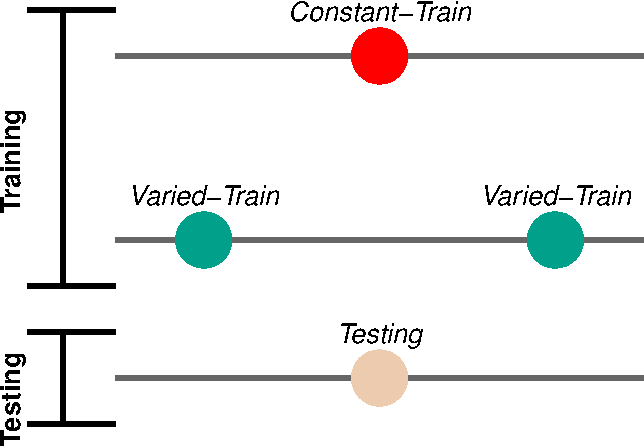
\includegraphics[keepaspectratio]{manuscript_files/figure-pdf/fig-ex-design1-1.pdf}}

}

\caption{\label{fig-ex-design1}A schematic representation of the Kerr \&
Booth (\citeproc{ref-kerrSpecificVariedPractice1978}{1978}) study
design. The varied group trained from two distances (2 and 4 feet),
while the constant group trained from a single distance (3 feet). Both
groups were tested from a distance of 3 feet. The varied group
outperformed the constant group at testing, despite the constant group
having exclusively practiced from the testing distance.}

\end{figure}%

Pitting varied against constant practice against each other on the home
turf of the constant group provides a compelling argument for the
benefits of varied training, as well as an interesting challenge for
theoretical accounts that posit generalization to occur as some function
of distance. However, despite its appeal this contrast is relatively
uncommon in the literature. It is unclear whether this may be cause for
concern over publication bias, or just researchers feeling the design is
too risky. A far more common design is to have separate constant groups
that each train exclusively from each of the conditions that the varied
group encounters
(\citeproc{ref-catalanoDistantTransferCoincident1984a}{Catalano \&
Kleiner, 1984}; \citeproc{ref-chuaPracticeVariabilityPromotes2019}{Chua
et al., 2019}; \citeproc{ref-mccrackenTestSchemaTheory1977}{McCracken \&
Stelmach, 1977};
\citeproc{ref-moxleySchemaVariabilityPractice1979}{Moxley, 1979};
\citeproc{ref-newellVariabilityPracticeTransfer1976}{Newell \& Shapiro,
1976}), or for a single constant group to train from just one of the
conditions experienced by the varied participants
(\citeproc{ref-pigottMotorSchemaStructure1984}{Pigott \& Shapiro, 1984};
\citeproc{ref-rollerVariablePracticeLenses2001}{Roller et al., 2001};
\citeproc{ref-wrisbergTrainingProductionNovel1984}{Wrisberg \& McLean,
1984}; \citeproc{ref-wrisbergDevelopingCoincidentTiming1983}{Wrisberg \&
Mead, 1983}). A less common contrast places the constant group training
in a region of the task space outside of the range of examples
experienced by the varied group, but distinct from the transfer
condition
(\citeproc{ref-wrisbergVariabilityPracticeHypothesis1987}{Wrisberg et
al., 1987}; \citeproc{ref-wulfVariabilityPracticeImplicit1997}{Wulf \&
Schmidt, 1997}). Of particular relevance to the current work is the
early study of Catalano \& Kleiner
(\citeproc{ref-catalanoDistantTransferCoincident1984a}{1984}), as theirs
was one of the earliest studies to investigate the influence of varied
vs.~constant training on multiple testing locations of graded distance
from the training condition. Participants were trained on coincident
timing task, in which subjects observe a series of lightbulbs turning on
sequentially at a consistent rate and attempt to time a button response
with the onset of the final bulb. The constant groups trained with a
single velocity of either 5,7,9, or 11 mph, while the varied group
trained from all 4 of these velocities. Participants were then assigned
to one of four possible generalization conditions, all of which fell
outside of the range of the varied training conditions -- 1, 3, 13 or 15
mph. As is often the case, the varied group performed worse during the
training phase. In the testing phase, the general pattern was for all
participants to perform worse as the testing conditions became further
away from the training conditions, but since the drop off in performance
as a function of distance was far less steep for the varied group, the
authors suggested that varied training induced a decremented
generalization gradient, such that the varied participants were less
affected by the change between training and testing conditions.

Benefits of varied training have also been observed in many studies
outside of the sensorimotor domain. Goode et al.
(\citeproc{ref-goodeSuperiorityVariableRepeated2008}{2008}) trained
participants to solve anagrams of 40 different words ranging in length
from 5 to 11 letters, with an anagram of each word repeated 3 times
throughout training, for a total of 120 training trials. Although
subjects in all conditions were exposed to the same 40 unique words
(i.e.~the solution to an anagram), participants in the varied group saw
3 different arrangements for each solution-word, such as DOLOF, FOLOD,
and OOFLD for the solution word FLOOD, whereas constant subjects would
train on three repetitions of LDOOF (spread evenly across training). Two
different constant groups were used. Both constant groups trained with
three repetitions of the same word scramble, but for constant group A,
the testing phase consisted of the identical letter arrangement to that
seen during training (e.g., LDOOF), whereas for constant group B, the
testing phase consisted of an arrangement they had not seen during
training, thus presenting them with a testing situation similar
situation to the varied group. At the testing stage, the varied group
outperformed both constant groups, a particularly impressive result,
given that constant group A had three prior exposures to the word
arrangement (i.e.~the particular permutation of letters) which the
varied group had not explicitly seen. However varied subjects in this
study did not exhibit the typical decrement in the training phase
typical of other varied manipulations in the literature, and achieved
higher levels of anagram solving accuracy by the end of training than
either of the constant groups -- solving two more anagrams on average
than the constant group. This might suggest that for tasks of this
nature where the learner can simply get stuck with a particular word
scramble, repeated exposure to the identical scramble might be less
helpful towards finding the solution than being given a different
arrangement of the same letters. This contention is supported by the
fact that constant group A, who was tested on the identical arrangement
as they experienced during training, performed no better at testing than
did constant group B, who had trained on a different arrangement of the
same word solution -- further suggesting that there may not have been a
strong identity advantage in this task.

In the domain of category learning, the constant vs.~varied comparison
is much less suitable. Instead, researchers will typically employ
designs where all training groups encounter numerous stimuli, but one
group experiences a greater number of unique exemplars
(\citeproc{ref-brunsteinPreparingNoveltyDiverse2011}{Brunstein \&
Gonzalez, 2011};
\citeproc{ref-doyleMetacognitiveMonitoringCategory2016}{Doyle \&
Hourihan, 2016};
\citeproc{ref-hoschPriorExperienceVariability2023}{Hosch et al., 2023};
\citeproc{ref-nosofskyModelguidedSearchOptimal2019}{Nosofsky et al.,
2019};
\citeproc{ref-wahlheimMetacognitiveJudgmentsRepetition2012}{Wahlheim et
al., 2012}), or designs where the number of unique training exemplars is
held constant, but one group trains with items that are more dispersed,
or spread out across the category space
(\citeproc{ref-bowmanTrainingSetCoherence2020}{Bowman \& Zeithamova,
2020}; \citeproc{ref-homaCategoryBreadthAbstraction1976}{Homa \&
Vosburgh, 1976}; \citeproc{ref-huHighvariabilityTrainingDoes2024}{Hu \&
Nosofsky, 2024};
\citeproc{ref-maddoxStimulusRangeDiscontinuity2011}{Maddox \& Filoteo,
2011}; \citeproc{ref-posnerGenesisAbstractIdeas1968}{Posner \& Keele,
1968}).

Much of the earlier work in this sub-area trained subjects on artificial
categories, such as dot patterns
(\citeproc{ref-homaCategoryBreadthAbstraction1976}{Homa \& Vosburgh,
1976}; \citeproc{ref-posnerGenesisAbstractIdeas1968}{Posner \& Keele,
1968}). A seminal study by Posner \& Keele
(\citeproc{ref-posnerGenesisAbstractIdeas1968}{1968}) trained
participants to categorize artificial dot patterns, manipulating whether
learners were trained with low variability examples clustered close to
the category prototypes (i.e.~low distortion training patterns), or
higher-variability patterns spread further away from the prototype
(i.e.~high-distortion patterns). Participants that received training on
more highly-distorted items showed superior generalization to novel high
distortion patterns in the subsequent testing phase. It should be noted
that unlike the sensorimotor studies discussed earlier, the Posner \&
Keele (\citeproc{ref-posnerGenesisAbstractIdeas1968}{1968}) study did
not present low-varied and high-varied participants with an equal number
of training trials, but instead had participants remain in the training
stage of the experiment until they reached a criterion level of
performance. This train-until-criterion procedure led to the
high-variability condition participants tending to complete a larger
number of training trials before switching to the testing stage. More
recent work (\citeproc{ref-huHighvariabilityTrainingDoes2024}{Hu \&
Nosofsky, 2024}) also used dot pattern categories, but matched the
number of training trials across conditions. Under this procedure,
higher-variability participants tended to reach lower levels of
performance by the end of the training stage. The results in the testing
phase were the opposite of Posner \& Keele
(\citeproc{ref-posnerGenesisAbstractIdeas1968}{1968}), with the
low-variability training group showing superior generalization to novel
high-distortion patterns (as well as generalization to novel patterns of
low or medium distortion levels). However, whether this discrepancy is
solely a result of the different training procedures is unclear, as the
studies also differed in the nature of the prototype patterns used.
Posner \& Keele (\citeproc{ref-posnerGenesisAbstractIdeas1968}{1968})
utilized simpler, recognizable prototypes (e.g., a triangle, the letter
M, the letter F), while Hu \& Nosofsky
(\citeproc{ref-huHighvariabilityTrainingDoes2024}{2024}) employed random
prototype patterns.

Recent studies have also begun utilizing more complex or realistic
stimuli when assessing the influence of variability on category
learning. Wahlheim et al.
(\citeproc{ref-wahlheimMetacognitiveJudgmentsRepetition2012}{2012})
conducted one such study. In a within-participants design, participants
were trained on bird categories with either many repetitions of a few
exemplars, or with few repetitions of many exemplars. Across four
different experiments, which were conducted to address an unrelated
question on metacognitive judgements, the researchers consistently found
that participants generalized better to novel species following training
with more unique exemplars (i.e.~higher variability), while high
repetition training produced significantly better performance
categorizing the specific species they had trained on. A variability
advantage was also found in the relatively complex domain of rock
categorization
(\citeproc{ref-nosofskyModelguidedSearchOptimal2019}{Nosofsky et al.,
2019}). For 10 different rock categories, participants were trained with
either many repetitions of 3 unique examples of each category, or few
repetitions of 9 unique examples, with an equal number of total training
trials in each group (the design also included 2 other conditions less
amenable to considering the impact of variation). The high-variability
group, trained with 9 unique examples, showed significantly better
generalization performance than the other conditions.

A distinct sub-literature within the category learning domain has
examined how the variability or dispersion of the categories themselves
influences generalization to ambiguous regions of the category space
(e.g., the region between the two categories). The general approach is
to train participants with examples from a high variability category and
a low variability category. Participants are then tested with novel
items located within ambiguous regions of the category space which allow
the experimenters to assess whether the difference in category
variability influenced how far participants generalize the category
boundaries. A. L. Cohen et al.
(\citeproc{ref-cohenCategoryVariabilityExemplar2001}{2001}) conducted
two experiments with this basic paradigm. In experiment 1, a low
variability category composed of 1 instance was compared against a
high-variability category of 2 instances in one condition, and 7
instances in another. In experiment 2 both categories were composed of 3
instances, but for the low-variability group the instances were
clustered close to each other, whereas the high-variability groups
instances were spread much further apart. Participants were tested on an
ambiguous novel instance that was located in between the two trained
categories. Both experiments provided evidence that participants were
much more likely to categorize the novel middle stimulus into the
category with greater variation.

Further observations of widened generalization following varied training
have since been observed in numerous investigations
(\citeproc{ref-hahnEffectsCategoryDiversity2005}{Hahn et al., 2005};
\citeproc{ref-hoschPriorExperienceVariability2023}{Hosch et al., 2023};
\citeproc{ref-hsuEffectsGenerativeDiscriminative2010}{Hsu \& Griffiths,
2010}; \citeproc{ref-perlmanFurtherAttemptsClarify2012}{Perlman et al.,
2012}; \citeproc{ref-sakamotoPuttingPsychologyBack2008}{Sakamoto et al.,
2008}; but see
\citeproc{ref-stewartEffectCategoryVariability2002}{Stewart \& Chater,
2002}; \citeproc{ref-yangCategoryVariabilityEffect2014}{L.-X. Yang \&
Wu, 2014}; and \citeproc{ref-seitzModelingCategoryVariability2023}{Seitz
et al., 2023}). The results of Sakamoto et al.
(\citeproc{ref-sakamotoPuttingPsychologyBack2008}{2008}) are noteworthy.
They first reproduced the basic finding of participants being more
likely to categorize an unknown middle stimulus into a training category
with higher variability. In a second experiment, they held the
variability between the two training categories constant and instead
manipulated the training sequence, such that the examples of one
category appeared in an ordered fashion, with very small changes from
one example to the other (the stimuli were lines that varied only in
length), whereas examples in the alternate category were shown in a
random order and thus included larger jumps in the stimulus space from
trial to trial. They found that the middle stimulus was more likely to
be categorized into the category that had been learned with a random
sequence, which was attributed to an increased perception of variability
which resulted from the larger trial to trial discrepancies.

The work of Hahn et al.
(\citeproc{ref-hahnEffectsCategoryDiversity2005}{2005}), is also of
particular interest to the present work. Their experimental design was
similar to previous studies, but they included a larger set of testing
items which were used to assess generalization both between the two
training categories as well as novel items located in the outer edges of
the training categories. During generalization testing, participants
were given the option to respond with ``neither'', in addition to
responses to the two training categories. The ``neither'' response was
included to test how far away in the stimulus space participants would
continue to categorize novel items as belonging to a trained category.
Consistent with prior findings, high-variability training resulted in an
increased probability of categorizing items in between the training
categories as belong to the high variability category. Additionally,
participants trained with higher variability also extended the category
boundary further out into the periphery than participants trained with a
lower variability category were willing to do. The author compared a
variety of similarity-based models based around the Generalized Context
Model
(\citeproc{ref-nosofskyAttentionSimilarityIdentificationcategorization1986}{Nosofsky,
1986}) to account for their results, manipulating whether a
response-bias or similarity-scaling parameter was fit separately between
variability conditions. No improvement in model fit was found by
allowing the response-bias parameter to differ between groups, however
the model performance did improve significantly when the similarity
scaling parameter was fit separately. The best fitting
similarity-scaling parameters were such that the high-variability group
was less sensitive to the distances between stimuli, resulting in
greater similarity values between their training items and testing
items. This model accounted for both the extended generalization
gradients of the varied participants, and for their poorer performance
in a recognition condition.

Variability has also been examined in the learning of higher-order
linguistic categories (\citeproc{ref-perryLearnLocallyThink2010}{Perry
et al., 2010}). In nine training sessions spread out over nine weeks
infants were trained on object labels in a naturalistic play setting.
All infants were introduced to three novel objects of the same category,
with participants in the ``tight'' condition being exposed to three
similar exemplars of the category, and participants in the varied
condition being exposed to three dissimilar objects of the same
category. Importantly, the similarity of the objects was carefully
controlled for by having a separate group of adult subjects provide
pairwise similarity judgements of the category objects prior to the
study onset. Multidimensional scaling was then performed to obtain the
coordinates of the objects psychological space, and out of the 10
objects for each category, the 3 most similar objects were selected for
the tight group and the three least similar objects for the varied
group, with the leftover four objects being retained for testing. By the
end of the nine weeks, all of the infants had learned the labels of the
training objects. In the testing phase, the varied group demonstrated
superior ability to correctly generalize the object labels to untrained
exemplars of the same category. More interesting was the superior
performance of the varied group on a higher order generalization task --
such that they were able to appropriately generalize the bias they had
learned during training for attending to the shape of objects to novel
solid objects, but not to non-solids. The tight training group, on the
other hand, tended to overgeneralize the shape bias, leading the
researchers to suggest that the varied training induced a more
context-sensitive understanding of when to apply their knowledge.

Of course, the relationship between training variability and transfer is
unlikely to be a simple function wherein increased variation is always
beneficial. Numerous studies have found null, or in some cases negative
effects of training variation
(\citeproc{ref-deloshExtrapolationSineQua1997}{DeLosh et al., 1997};
\citeproc{ref-sinkeviciuteRoleInputVariability2019}{Sinkeviciute et al.,
2019}; \citeproc{ref-vanrossumSchmidtSchemaTheory1990}{Van Rossum,
1990}; \citeproc{ref-wrisbergVariabilityPracticeHypothesis1987}{Wrisberg
et al., 1987}), and many more have suggested that the benefits of
variability may depend on additional factors such as prior task
experience, the order of training trials, or the type of transfer being
measured (\citeproc{ref-bernikerEffectsTrainingBreadth2014}{Berniker et
al., 2014};
\citeproc{ref-braithwaiteEffectsVariationPrior2015}{Braithwaite \&
Goldstone, 2015}; \citeproc{ref-hahnEffectsCategoryDiversity2005}{Hahn
et al., 2005}; \citeproc{ref-lavanEffectsHighVariability2019}{Lavan et
al., 2019}; \citeproc{ref-northEffectConsistentVaried2019}{North et al.,
2019}; \citeproc{ref-sadakataIndividualAptitudeMandarin2014}{Sadakata \&
McQueen, 2014};
\citeproc{ref-zamanPerceptualVariabilityImplications2021}{Zaman et al.,
2021}).

In an example of a more complex influence of training variation,
(\citeproc{ref-braithwaiteEffectsVariationPrior2015}{Braithwaite \&
Goldstone, 2015}) trained participants on example problems involving the
concept of sampling with replacement (SWR). Training consisted of
examples that were either highly similar in their semantic context
(e.g., all involving people selecting objects) or in which the surface
features were varied between examples (e.g., people choosing objects AND
objects selected in a sequence). The experimenters also surveyed how
much prior knowledge each participant had with SWR. They found that
whether variation was beneficial depended on the prior knowledge of the
participants -- such that participants with some prior knowledge
benefited from varied training, whereas participants with minimal prior
knowledge performed better after training with similar examples. The
authors hypothesized that to benefit from varied examples, participants
must be able to detect the structure common to the diverse examples, and
that participants with prior knowledge are more likely to be sensitive
to such structure, and thus to benefit from varied training. To test
this hypothesis more directly, the authors conducted a 2nd experiment,
wherein they controlled prior knowledge by exposing some subjects to a
short graphical or verbal pre-training lesson, designed to increase
sensitivity to the training examples. Consistent with their hypothesis,
participants exposed to the structural sensitivity pre-training
benefited more from varied training than the controls participants who
benefited more from training with similar examples. Interactions between
prior experience and the influence of varied training have also been
observed in sensorimotor learning
(\citeproc{ref-delreyEffectsContextualInterference1982}{Del Rey et al.,
1982};
\citeproc{ref-guadagnoliRelationshipContextualInterference1999}{Guadagnoli
et al., 1999}). Del Rey et al.
(\citeproc{ref-delreyEffectsContextualInterference1982}{1982}) recruited
participants who self-reported either extensive, or very little
experience with athletic activities, and then trained participants on a
coincident timing task with either a single constant training velocity,
or with one of several varied training procedures. Unsurprisingly,
athlete participants had superior performance during training,
regardless of condition, and training performance was superior for all
subjects in the constant group. Of greater interest is the pattern of
testing results from novel transfer conditions. Among the
athlete-participants, transfer performance was best for those who
received variable training. Non-athletes showed the opposite pattern,
with superior performance for those who had constant training.

\subsection{Existing Theoretical
Frameworks}\label{existing-theoretical-frameworks}

Several theoretical frameworks have been proposed to conceptually
explain the effects of varied training on learning and generalization.
Schema theory (described in more detail above), posts that varied
practice leads to the formation of more flexible motor schemas, which
then facilitate generalization
(\citeproc{ref-schmidtSchemaTheoryDiscrete1975}{Schmidt, 1975}). The
desirable difficulties framework
(\citeproc{ref-bjorkMakingThingsHard2011}{Bjork \& Bjork, 2011};
\citeproc{ref-soderstromLearningPerformanceIntegrative2015}{Soderstrom
\& Bjork, 2015}) proposes that variable practice conditions may impair
initial performance but then enhance longer-term retention and transfer.
Similarly, the challenge point framework
(\citeproc{ref-guadagnoliChallengePointFramework2004}{Guadagnoli \& Lee,
2004}) contends that training variation induces optimal learning occurs
insofar as it causes the difficulty of practice tasks to be
appropriately matched to the learner's capabilities, but may also be
detrimental if the amount of variation causes the task to be too
difficult.

While these frameworks offer valuable conceptual accounts, there has
been a limited application of computational modeling efforts aimed at
quantitatively assessing and comparing the learning and generalization
mechanisms which may be underlying the influence of variability in
visuomotor skill learning. In contrast, the effects of variability have
received more formal computational treatment in other domains, such as
category learning Hu \& Nosofsky
(\citeproc{ref-huHighvariabilityTrainingDoes2024}{2024}), language
learning (\citeproc{ref-jonesDensityDistinctivenessEarly2020}{Jones \&
Brandt, 2020}), and function learning
(\citeproc{ref-deloshExtrapolationSineQua1997}{DeLosh et al., 1997}). A
primary goal of the current dissertation is to address this gap by
adapting and applying modeling approaches from these other domains to
investigate the effects of training variability in visuomotor skill
learning and function learning tasks.

\subsection{The current work}\label{the-current-work}

The overarching purpose of this dissertation is to investigate the
effects of training variability on learning and generalization within
visuomotor skill learning and function learning. Our investigation is
structured into two main projects, each employing distinct experimental
paradigms and computational modeling frameworks to elucidate how and
when variability in training enhances or impedes subsequent
generalization.

In Project 1, we investigated the influence of varied practice in a
simple visuomotor projectile launching task. Experiments 1 and 2
compared the performance of constant and varied training groups to
assess potential benefits of variability on transfer to novel testing
conditions. To account for the observed empirical effects, we introduced
the Instance-based Generalization with Adaptive Similarity (IGAS) model.
IGAS provides a novel computational approach for quantifying the
similarity between training experiences and transfer conditions, while
also allowing for variability to influence the generalization gradient
itself.

Project 2 will focus on the domain of function learning and in
particular the issue of extrapolation. Function learning research
examines how people acquire and generalize knowledge about continuous
input-output relationships, and the factors influencing extrapolation to
novel inputs following an initial learning phase. The domain of function
learning has yielded influential computational models, including the
Associative Learning Model (ALM) and the Extrapolation-Association Model
(EXAM)(\citeproc{ref-busemeyerLearningFunctionalRelations1997}{Busemeyer
et al., 1997}), which have successfully accounted for human learning,
interpolation, and extrapolation in numerous
investigations(\citeproc{ref-deloshExtrapolationSineQua1997}{DeLosh et
al., 1997};
\citeproc{ref-mcdanielPredictingTransferPerformance2009}{McDaniel et
al., 2009}; \citeproc{ref-mcdanielConceptualBasisFunction2005}{McDaniel
\& Busemeyer, 2005}). However, the influence of training variability on
function learning, particularly in visuomotor function learning tasks,
remains relatively unexplored. Project 2 of this dissertation will
address this gap by investigating how constant and varied training
regimes affect learning, discrimination, and extrapolation in a novel
visuomotor function learning task. We will leverage the ALM and EXAM
models, fitted to individual participant data using advanced Bayesian
techniques, to provide a detailed computational account of the observed
empirical patterns.

\newpage{}

\section{Project 1}\label{project-1}

This project is based on the following publication:

Gorman, T. E., \& Goldstone, R. L. (2022). An instance-based model
account of the benefits of varied practice in visuomotor skill.
\emph{Cognitive Psychology}, 137, 101491.

\subsection{Abstract}\label{abstract}

Exposing learners to variability during training has been demonstrated
to improve performance in subsequent transfer testing. Such variability
benefits are often accounted for by assuming that learners are
developing some general task schema or structure. However, much of this
research has neglected to account for differences in similarity between
varied and constant training conditions. In a between-groups
manipulation, we trained participants on a simple projectile launching
task, with either varied or constant conditions. We replicate previous
findings showing a transfer advantage of varied over constant training.
Furthermore, we show that a standard similarity model is insufficient to
account for the benefits of variation, but, if the model is adjusted to
assume that varied learners are tuned towards a broader generalization
gradient, then a similarity-based model is sufficient to explain the
observed benefits of variation. Our results therefore suggest that some
variability benefits can be accommodated within instance-based models
without positing the learning of some schemata or structure.

\subsection{Introduction}\label{introduction-1}

\subsubsection{Similarity and instance-based approaches to transfer of
learning}\label{similarity-and-instance-based-approaches-to-transfer-of-learning}

Early models of learning often assumed that discrete experiences with
some task or category were not stored individually in memory, but
instead promoted the formation of a summary representation, often
referred to as a prototype or schema, and that exposure to novel
examples would then prompt the retrieval of whichever preexisting
prototype was most similar. In addition to being a landmark study on the
influence of training variability, Posner \& Keele
(\citeproc{ref-posnerGenesisAbstractIdeas1968}{1968}) (described above)
also put forward an influential argument concerning the nature of the
mental representations acquired during learning - namely that learners
tend to abstract a prototype, or aggregate representation of the dot
pattern categories, rather than encoding each individual stimulus.
Recall that participants are trained on only on distortions of the
category prototypes (e.g., low, medium or high distortions), never
encountering the exact prototypes during the training stage. Then, in
the testing phase, participants are tested with the prototype patterns,
their old training items, and novel low, medium and high distortions.
The authors found that participants had the highest testing accuracy for
the previously unseen prototype patterns, followed by the old training
items, and then the novel low, medium and high distortions. The authors
interpreted this pattern as evidence that participants had acquired
prototype representation of the category, as opposed to storing each
individual training instance, and that generalization was based on the
similarity of the testing items to the learned prototype
representations. Posner \& Keele
(\citeproc{ref-posnerGenesisAbstractIdeas1968}{1968}) has been extremely
influential, and continues to be cited as evidence that prototype
abstraction underlies the benefits of varied training. It's also
referenced as a key influence in the development of the ``Schema Theory
of Motor Learning'' Schmidt
(\citeproc{ref-schmidtSchemaTheoryDiscrete1975}{1975}), which in turn
influenced decades of research on the potential benefits of varied
training in motor skill learning. However, a number of the core
assumptions utilized by Posner \& Keele
(\citeproc{ref-posnerGenesisAbstractIdeas1968}{1968}) were later called
into question both empirically and with competing theoretical accounts
(\citeproc{ref-hintzmanMINERVASimulationModel1984}{Hintzman, 1984},
\citeproc{ref-hintzmanSchemaAbstractionMultipletrace1986}{1986};
\citeproc{ref-knappTheoryCategorizationBased1984}{Knapp \& Anderson,
1984};
\citeproc{ref-mcclellandDistributedMemoryRepresentation1985}{McClelland
\& Rumelhart, 1985};
\citeproc{ref-nosofskyInvestigationsExemplarBasedConnectionist1992}{Nosofsky
\& Kruschke, 1992};
\citeproc{ref-palmeriCentralTendenciesExtreme2001}{Palmeri \& Nosofsky,
2001}; \citeproc{ref-zakiHighdistortionEnhancementEffect2007}{Zaki \&
Nosofsky, 2007}). Palmeri \& Nosofsky
(\citeproc{ref-palmeriCentralTendenciesExtreme2001}{2001}) demonstrated
both the dangers of assuming that psychological representations mimic
the metric stimulus space, as well the viability of models with simpler
representational assumptions. These authors conducted a near replication
of the Posner \& Keele
(\citeproc{ref-posnerGenesisAbstractIdeas1968}{1968}) study, but also
had participants provide similarity judgements of the dot pattern
stimuli after completing the training phase. A multidimensional scaling
analysis of the similarity judgements revealed that the psychological
representations of the prototype stimuli were not located in the middle
of the training stimuli, but were instead extreme points in the
psychological space. The authors also demonstrated the generalization
patterns of Posner \& Keele
(\citeproc{ref-posnerGenesisAbstractIdeas1968}{1968}) could be accounted
for by an exemplar-based model, without any need to assume the
abstraction of a prototype.

Instance-based, or exemplar-based models generally assume that learners
encode each experience with a task as a separate
instance/exemplar/trace, and that each encoded trace is in turn compared
against novel stimuli
(\citeproc{ref-estesClassificationCognition1994}{Estes, 1994};
\citeproc{ref-hintzmanMINERVASimulationModel1984}{Hintzman, 1984};
\citeproc{ref-jamiesonInstanceTheoryDomaingeneral2022}{Jamieson et al.,
2022}; \citeproc{ref-medinContextTheoryClassification1978}{Medin \&
Schaffer, 1978};
\citeproc{ref-nosofskyAttentionSimilarityIdentificationcategorization1986}{Nosofsky,
1986}). As the number of stored instances increases, so does the
likelihood that some previously stored instance will be retrieved to aid
in the performance of a novel task. Stored instances are retrieved in
the context of novel stimuli or tasks if they are sufficiently similar,
thus suggesting that the process of computing similarity is of central
importance to generalization.

Similarity, defined in this literature as a function of psychological
distance between instances or categories, has provided a successful
account of generalization across numerous tasks and domains. In an
influential study demonstrating an ordinal similarity effect,
experimenters employed a numerosity judgment task in which participants
quickly report the number of dots flashed on a screen. Performance (in
terms of response times to new patterns) on novel dot configurations
varied as an inverse function of their similarity to previously trained
dot configurations Palmeri
(\citeproc{ref-palmeriExemplarSimilarityDevelopment1997}{1997}). That
is, performance was better on novel configurations moderately similar to
trained configurations than to configurations with low-similarity, and
also better on low-similarity configurations than to even less similar,
unrelated configurations. Instance-based similarity approaches have had
some success accounting for performance in certain sub-domains of motor
learning (\citeproc{ref-cohenWhereGraspsAre2004}{R. G. Cohen \&
Rosenbaum, 2004};
\citeproc{ref-crumpEpisodicContributionsSequential2010}{Crump \& Logan,
2010}; \citeproc{ref-meighWhatMemoryRepresentation2018}{Meigh et al.,
2018}; \citeproc{ref-poldrackRelationshipSkillLearning1999}{Poldrack et
al., 1999}; \citeproc{ref-wifallReachingResponseSelection2017}{Wifall et
al., 2017}). Crump \& Logan
(\citeproc{ref-crumpEpisodicContributionsSequential2010}{2010}) trained
participants to type words on an unfamiliar keyboard, while constraining
the letters composing the training words to a pre-specified letter set.
Following training, typing speed was tested on previously experienced
words composed of previously experienced letters; novel words composed
of letters from the trained letter set; and novel words composed of
letters from an untrained letter set. Consistent with an instance-based
account, transfer performance was graded such that participants were
fastest at typing the words they had previously trained on, followed by
novel words composed of letters they had trained on, and slowest
performance for new words composed of untrained letters.

\subsubsection{Issues with Previous
Research}\label{issues-with-previous-research}

Although the benefits of training variation in visuomotor skill learning
have been observed many times, null findings have also been repeatedly
found, leading some researchers to question the veracity of the
variability of practice hypothesis
(\citeproc{ref-newellSchemaTheory19752003}{Newell, 2003};
\citeproc{ref-vanrossumSchmidtSchemaTheory1990}{Van Rossum, 1990}).
Critics have also pointed out that investigations of the effects of
training variability, of the sort described above, often fail to control
for the effect of similarity between training and testing conditions.
For training tasks in which participants have numerous degrees of
freedom (e.g., projectile throwing tasks where participants control the
x and y velocity of the projectile), varied groups are likely to
experience a wider range of the task space over the course of their
training (e.g., more unique combinations of x and y velocities).
Experimenters may attempt to account for this possibility by ensuring
that the training location(s) of the varied and constant groups are an
equal distance away from the eventual transfer locations, such that
their training throws are, on average, equally similar to throws that
would lead to good performance at the transfer locations. However, even
this level of experimental control may still be insufficient to rule out
the effect of similarity on transfer. Given that psychological
similarity is typically best described as either a Gaussian or
exponentially decaying function of psychological distance
(\citeproc{ref-ennisMultidimensionalStochasticTheory1988}{Ennis et al.,
1988};
\citeproc{ref-ghahramaniGeneralizationLocalRemappings1996}{Ghahramani et
al., 1996}; \citeproc{ref-loganInstanceTheoryAutomatization1988}{Logan,
1988}; \citeproc{ref-nosofskySimilarityScalingCognitive1992}{Nosofsky,
1992}; \citeproc{ref-shepardUniversalLawGeneralization1987}{Shepard,
1987}; \citeproc{ref-thoroughmanRapidReshapingHuman2005}{Thoroughman \&
Taylor, 2005}), it is plausible that a subset of the most similar
training instances could have a disproportionate impact on
generalization to transfer conditions, even if the average distance
between training and transfer conditions is identical between groups.
Figure~\ref{fig-toy-model1} demonstrates the consequences of a
generalization gradient that drops off as a Gaussian function of
distance from training, as compared to a linear drop-off.

\begin{figure}

\centering{

\pandocbounded{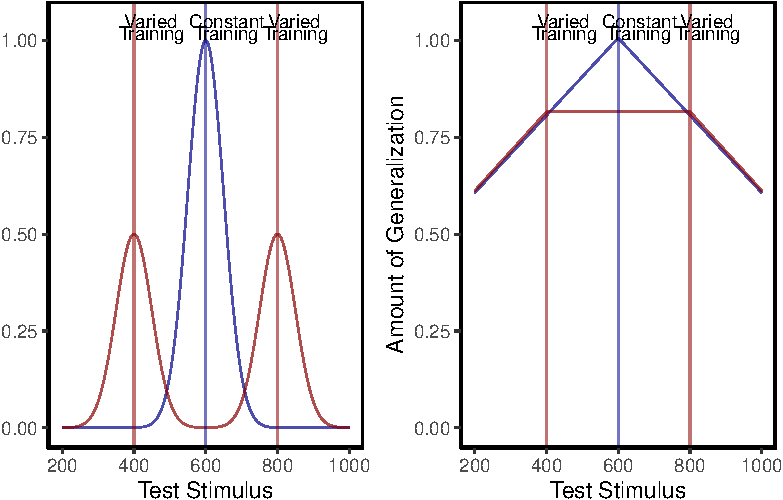
\includegraphics[keepaspectratio]{manuscript_files/figure-pdf/fig-toy-model1-1.pdf}}

}

\caption{\label{fig-toy-model1}Left panel- Generalization predicted from
a simple model that assumes a linear generalization function. A varied
group (red vertical lines indicate the 2 training locations) trained
from positions 400 and 800, and a constant group (blue vertical line),
trained from position 600. Right panel- if a Gaussian generalization
function is assumed, then varied training (400, 800) is predicted to
result in better generalization to positions close to 400 and 800 than
does constant training at 600. (For interpretation of the references to
color in this figure legend, the reader is referred to the web version
of this article.)}

\end{figure}%

In addition to largely overlooking the potential for non-linear
generalization to confound interpretations of training manipulations,
the visuomotor skill learning literature also rarely considers
alternatives to schema representations
(\citeproc{ref-chamberlinMemoryRepresentationMotor1992}{Chamberlin \&
Magill, 1992b}). Although schema-theory remains influential within
certain literatures, instance or exemplar-based models have accounted
for human behavior across myriad domains
(\citeproc{ref-jamiesonInstanceTheoryDomaingeneral2022}{Jamieson et al.,
2022}; \citeproc{ref-loganInstanceTheoryAttention2002a}{Logan, 2002}).
As mentioned above, instance based accounts have been shown to perform
well on a variety of different tasks with motoric components
(\citeproc{ref-crumpEpisodicContributionsSequential2010}{Crump \& Logan,
2010}; \citeproc{ref-gandolfoMotorLearningField1996a}{Gandolfo et al.,
1996}; \citeproc{ref-meighWhatMemoryRepresentation2018}{Meigh et al.,
2018}; \citeproc{ref-rosenbaumPlanningReachesEvaluating1995}{Rosenbaum
et al., 1995}; \citeproc{ref-vandamMappingShapeVisuomotor2015}{van Dam
\& Ernst, 2015}). However, such accounts have received little attention
within the subdomain of visuomotor skill learning focused on the
benefits of varied training.

The present work examines whether the commonly observed benefits of
varied training can be accounted for by a theoretically motivated
measure of the similarity between training throws and the testing
solution space. We first attempt to replicate previous work finding an
advantage of varied training over constant training in a projectile
launching task. We then examine the extent to which this advantage can
be explained by an instance-based similarity model.

\subsection{Experiment 1}\label{experiment-1}

\subsubsection{Methods}\label{methods}

\paragraph{Sample Size Estimation}\label{sample-size-estimation}

To obtain an independent estimate of effect size, we identified previous
investigations which included between-subjects contrasts of varied and
constant conditions following training on an accuracy-based projectile
launching task (\citeproc{ref-chuaPracticeVariabilityPromotes2019}{Chua
et al., 2019};
\citeproc{ref-goodwinEffectDifferentQuantities1998}{Goodwin et al.,
1998}; \citeproc{ref-kerrSpecificVariedPractice1978}{Kerr \& Booth,
1978}; \citeproc{ref-wulfEffectTypePractice1991}{Wulf, 1991}). We then
averaged effects across these studies, yielding a Cohen's f =.43. The
GPower 3.1 software package
(\citeproc{ref-faulStatisticalPowerAnalyses2009}{Faul et al., 2009}) was
then used to determine that a power of 80\% requires a sample size of at
least 23 participants per condition. All experiments reported in the
present manuscript exceed this minimum number of participants per
condition.

\paragraph{Participants}\label{participants}

Participants were recruited from an undergraduate population that is
63\% female and consists almost entirely of individuals aged 18 to 22
years. A total of 110 Indiana University psychology students
participated in Experiment 1. We subsequently excluded 34 participants
for poor performance on one of the dependent measures of the task (2.5-3
standard deviations worse than the median subject at the task) or for
displaying a pattern of responses that was clearly indicative of a lack
of engagement with the task (e.g., simply dropping the ball on each
trial rather than throwing it at the target), or for reporting that they
completed the experiment on a phone or tablet device, despite the
instructions not to use one of these devices. A total of 74 participants
were retained for the final analyses, 35 in the varied group and 39 in
the constant group.

\paragraph{Task}\label{task}

The experimental task was programmed in JavaScript, using packages from
the Phaser physics engine (https://phaser.io) and the jsPsych library
(\citeproc{ref-deleeuwJsPsychJavaScriptLibrary2015}{de Leeuw, 2015}).
The stimuli, presented on a black background, consisted of a circular
blue ball - controlled by the participant via the mouse or trackpad
cursor; a rectangular green target; a red rectangular barrier located
between the ball and the target; and an orange square within which the
participant could control the ball before releasing it in a throw
towards the target. Because the task was administered online, the
absolute distance between stimuli could vary depending on the size of
the computer monitor being used, but the relative distance between the
stimuli was held constant. Likewise, the distance between the center of
the target and the training and testing locations was scaled such that
relative distances were preserved regardless of screen size. For the
sake of brevity, subsequent mentions of this relative distance between
stimuli, or the position where the ball landed in relation to the center
of the target, will be referred to simply as distance.
Figure~\ref{fig-IGAS_Methods} displays the layout of the task, as it
would appear to a participant at the start of a trial, with the ball
appearing in the center of the orange square. Using a mouse or trackpad,
participants click down on the ball to take control of the ball,
connecting the movement of the ball to the movement of the cursor.
Participants can then ``wind up'' the ball by dragging it (within the
confines of the orange square) and then launch the ball by releasing the
cursor. If the ball does not land on the target, participants are
presented with feedback in red text at the top right of the screen,
specifying how many scaled units away the ball was from the center of
the target. If the ball was thrown outside of the boundary of the screen
participants are given feedback as to how far away from the target
center the ball would have been if it had continued its trajectory. If
the ball strikes the barrier (from the side or by landing on top),
feedback is presented telling participants to avoid hitting the barrier.
If participants drag the ball outside of the orange square before
releasing it, the trial terminates, and they are reminded to release the
ball within the orange square. If the ball lands on the target, feedback
is presented in green text, confirming that the target was hit, and
presenting additional feedback on how many units away the ball was from
the exact center of the target.

\href{https://pcl.sitehost.iu.edu/tg/demos/igas_expt1_demo.html}{Link to
abbreviated example of task}.

\begin{figure}

\centering{

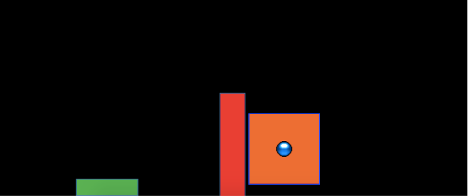
\includegraphics[width=0.6\linewidth,height=\textheight,keepaspectratio]{../Assets/methodsFig1.png}

}

\caption{\label{fig-IGAS_Methods}The stimuli of the task consisted of a
blue ball, which the participants would launch at the green target,
while avoiding the red barrier. On each trial, the ball would appear in
the center of the orange square, with the position of the orange square
varying between experimental conditions. Participants were constrained
to release the ball within the square.}

\end{figure}%

\paragraph{Procedure}\label{procedure}

Participants first electronically consented to participate, and then
read instructions for the task which explained how to control the ball,
and the goal of throwing the ball as close to the center of the target
as possible. The training phase was split into 10 blocks of 20 trials,
for a total of 200 training trials. Participants in the constant
condition trained exclusively from a single location (760 scaled units
from the target center). Participants in the varied condition trained
from two locations (610 and 910 scaled units from the target center),
encountering each location 100 times. The sequence of throwing locations
was pseudo-random for the varied group, with the constraint that within
every block of 20 training throws both training locations would occur 10
times. Participants in both conditions also received intermittent
testing trials after every 20 training trials. Intermittent testing
trials provided no feedback of any kind. The ball would disappear from
view as soon as it left the orange square, and participants were
prompted to start the next trial without receiving any information about
the accuracy of the throw. Each intermittent testing stage consisted of
two trials from each of the three training positions (i.e.~all
participants executed two trials each from Positions 610, 760, and 910
during each of the 10 intermittent testing stages). Following training,
all participants completed a final testing phase from four positions: 1)
their training location, 2) the training location(s) of the other group,
3) a location novel to both groups. The testing phase consisted of 15
trials from each of the four locations, presented in a randomized order.
All trials in the final testing phase included feedback. After finishing
the final testing portion of the study, participants were queried as to
whether they completed the study using a mouse, a trackpad, or some
other device (this information was used in the exclusion process
described above). Finally, participants were debriefed as to the
hypotheses and manipulation of the study.

\subsubsection{Results}\label{results}

\paragraph{Data Processing and Statistical
Packages}\label{data-processing-and-statistical-packages}

To prepare the data, we removed trials that were not easily
interpretable as performance indicators in our task. Removed trials
included: 1) those in which participants dragged the ball outside of the
orange starting box without releasing it, 2) trials in which
participants clicked on the ball, and then immediately released it,
causing the ball to drop straight down, 3) outlier trials in which the
ball was thrown more than 2.5 standard deviations further than the
average throw (calculated separately for each throwing position), and 4)
trials in which the ball struck the barrier. The primary measure of
performance used in all analyses was the absolute distance away from the
center of the target. The absolute distance was calculated on every
trial, and then averaged within each subject to yield a single
performance score, for each position. A consistent pattern across
training and testing phases in both experiments was for participants to
perform worse from throwing positions further away from the target -- a
pattern which we refer to as the difficulty of the positions. However,
there were no interactions between throwing position and training
conditions, allowing us to collapse across positions in cases where
contrasts for specific positions were not of interest. All data
processing and statistical analyses were performed in R version 4.32
(\citeproc{ref-rcoreteamLanguageEnvironmentStatistical2020}{Team,
2020}). ANOVAs for group comparisons were performed using the rstatix
package
(\citeproc{ref-kassambaraRstatixPipeFriendlyFramework2021a}{Kassambara,
2021}).

\paragraph{Training Phase}\label{training-phase}

Figure~\ref{fig-IGAS_Training1} below shows aggregate training
performance binned into three stages representing the beginning, middle,
and end of the training phase. Because the two conditions trained from
target distances that were not equally difficult, it was not possible to
directly compare performance between conditions in the training phase.
Our focus for the training data analysis was instead to establish that
participants did improve their performance over the course of training,
and to examine whether there was any interaction between training stage
and condition. Descriptive statistics for the intermittent testing phase
are provided in the supplementary materials.

We performed an ANOVA comparison with stage as a within-group factor and
condition as between-group factor. The analysis revealed a significant
effect of training stage F(2,142)=62.4, p\textless.001, \(\eta^{2}_G\) =
.17, such that performance improved over the course of training. There
was no significant effect of condition F(1,71)=1.42, p=.24,
\(\eta^{2}_G\) = .02, and no significant interaction between condition
and training stage, F(2,142)=.10, p=.91, \(\eta^{2}_G\) \textless{} .01.

\begin{figure}

\centering{

\pandocbounded{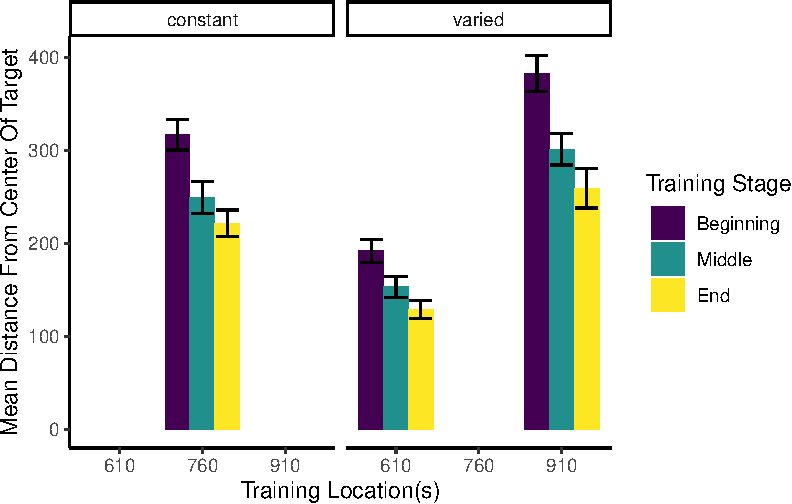
\includegraphics[keepaspectratio]{manuscript_files/figure-pdf/fig-IGAS_Training1-1.pdf}}

}

\caption{\label{fig-IGAS_Training1}Training performance for varied and
constant participants binned into three stages. Shorter bars indicate
better performance (ball landing closer to the center of the target).
Error bars indicate standard error of the mean.}

\end{figure}%

\paragraph{Testing Phase}\label{testing-phase}

In Experiment 1, a single constant-trained group was compared against a
single varied-trained group. At the transfer phase, all participants
were tested from 3 positions: 1) the positions(s) from their own
training, 2) the training position(s) of the other group, and 3) a
position novel to both groups. Overall, group performance was compared
with a mixed type III ANOVA, with condition (varied vs.~constant) as a
between-subject factor and throwing location as a within-subject
variable. The effect of throwing position was strong, F(3,213) = 56.12,
p\textless.001, η2G = .23. The effect of training condition was
significant F(1,71)=8.19, p\textless.01, η2G = .07. There was no
significant interaction between group and position, F(3,213)=1.81,
p=.15, η2G = .01.

\begin{figure}

\centering{

\pandocbounded{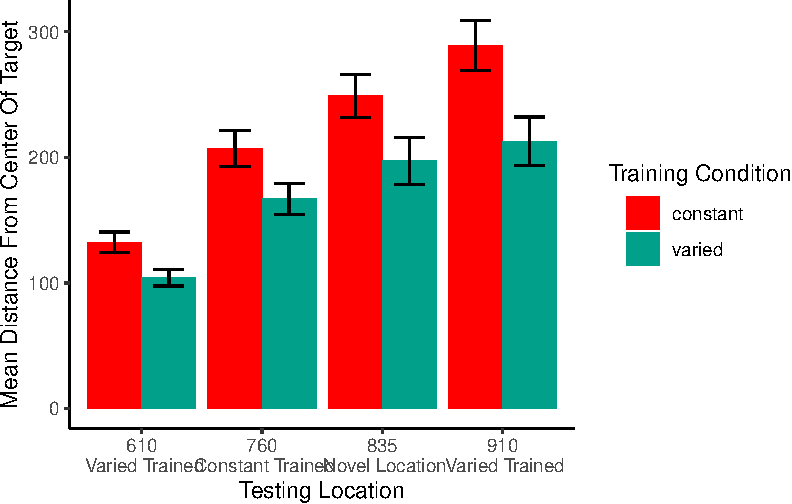
\includegraphics[keepaspectratio]{manuscript_files/figure-pdf/fig-IGAS_Testing1-1.pdf}}

}

\caption{\label{fig-IGAS_Testing1}Testing performance for each of the 4
testing positions, compared between training conditions. Positions 610
and 910 were trained on by the varied group, and novel for the constant
group. Position 760 was trained on by the constant group, and novel for
the varied group. Position 835 was novel for both groups. Shorter bars
are indicative of better performance (the ball landing closer to the
center of the target). Error bars indicate standard error of the mean.}

\end{figure}%

\hfill\break
\hfill\break

\begin{longtable}[]{@{}lll@{}}

\caption{\label{tbl-IGAS_Table1}Testing performance for varied and
constant groups in experiment 1. Mean absolute deviation from the center
of the target, with standard deviations in parenthesis.}

\tabularnewline

\toprule\noalign{}
Position & Constant & Varied \\
\midrule\noalign{}
\endhead
\bottomrule\noalign{}
\endlastfoot
610 & 132.48(50.85) & 104.2(38.92) \\
760 & 207.26(89.19) & 167.12(72.29) \\
835 & 249.13(105.92) & 197.22(109.71) \\
910 & 289.36(122.48) & 212.86(113.93) \\

\end{longtable}

\subsubsection{Discussion}\label{discussion}

In Experiment 1, we found that varied training resulted in superior
testing performance than constant training, from both a position novel
to both groups, and from the position at which the constant group was
trained, which was novel to the varied condition. The superiority of
varied training over constant training even at the constant training
position is of particular note, given that testing at this position
should have been highly similar for participants in the constant
condition. It should also be noted, though, that testing at the constant
trained position is not identical to training from that position, given
that the context of testing is different in several ways from that of
training, such as the testing trials from the different positions being
intermixed, as well as a simple change in context as a function of time.
Such contextual differences will be further considered in the General
Discussion.

In addition to the variation of throwing position during training, the
participants in the varied condition of Experiment 1 also received
training practice from the closest/easiest position, as well as from the
furthest/most difficult position that would later be encountered by all
participants during testing. The varied condition also had the potential
advantage of interpolating both of the novel positions from which they
would later be tested. Experiment 2 thus sought to address these issues
by comparing a varied condition to multiple constant conditions.

\subsection{Experiment 2}\label{experiment-2}

In Experiment 2, we sought to replicate our findings from Experiment 1
with a new sample of participants, while also addressing the possibility
of the pattern of results in Experiment 1 being explained by some
idiosyncrasy of the particular training location of the constant group
relative to the varied group. To this end, Experiment 2 employed the
same basic procedure as Experiment 1, but was designed with six separate
constant groups each trained from one of six different locations (400,
500, 625, 675, 800, or 900), and a varied group trained from two
locations (500 and 800). Participants in all seven groups were then
tested from each of the 6 unique positions.

\subsubsection{Methods}\label{methods-1}

\paragraph{Participants}\label{participants-1}

A total of 306 Indiana University psychology students participated in
Experiment 2, which was also conducted online. As was the case in
Experiment 1, the undergraduate population from which we recruited
participants was 63\% female and primarily composed of 18--22-year-old
individuals. Using the same procedure as Experiment 1, we excluded 98
participants for exceptionally poor performance at one of the dependent
measures of the task, or for displaying a pattern of responses
indicative of a lack of engagement with the task. A total of 208
participants were included in the final analyses with 31 in the varied
group and 32, 28, 37, 25, 29, 26 participants in the constant groups
training from location 400, 500, 625, 675, 800, and 900, respectively.
All participants were compensated with course credit.

\paragraph{Task and Procedure}\label{task-and-procedure}

The task of Experiment 2 was identical to that of Experiment 1, in all
but some minor adjustments to the height of the barrier, and the
relative distance between the barrier and the target. Additionally, the
intermittent testing trials featured in experiment 1 were not utilized
in Experiment 2. An abbreviated demo of the task used for Experiment 2
can be found at
(https://pcl.sitehost.iu.edu/tg/demos/igas\_expt2\_demo.html).

The procedure for Experiment 2 was also quite similar to Experiment 1.
Participants completed 140 training trials, all of which were from the
same position for the constant groups and split evenly (70 trials each -
randomized) for the varied group. In the testing phase, participants
completed 30 trials from each of the six locations that had been used
separately across each of the constant groups during training. Each of
the constant groups thus experienced one trained location and five novel
throwing locations in the testing phase, while the varied group
experiences 2 previously trained, and 4 novel locations.

\subsubsection{Results}\label{results-1}

\paragraph{Data Processing and Statistical
Packages}\label{data-processing-and-statistical-packages-1}

After confirming that condition and throwing position did not have any
significant interactions, we standardized performance within each
position, and then average across position to yield a single performance
measure per participant. This standardization did not influence our
pattern of results. As in Experiment 1, we performed type III ANOVAs due
to our unbalanced design, however the pattern of results presented below
is not altered if type 1 or type III tests are used instead. The
statistical software for the primary analyses was the same as for
Experiment 1. Individual learning rates in the testing phase, compared
between groups in the supplementary analyses, were fit using the TEfit
package in R
(\citeproc{ref-cochraneTEfitsNonlinearRegression2020}{Cochrane, 2020}).

\paragraph{Training Phase}\label{training-phase-1}

The different training conditions trained from positions that were not
equivalently difficult and are thus not easily amenable to comparison.
As previously stated, the primary interest of the training data is
confirmation that some learning did occur. Figure~\ref{fig-e2train}
depicts the training performance of the varied group alongside that of
the aggregate of the six constant groups (5a), and each of the 6
separate constant groups (5b). An ANOVA comparison with training stage
(beginning, middle, end) as a within-group factor and group (the varied
condition vs.~the 6 constant conditions collapsed together) as a
between-subject factor revealed no significant effect of group on
training performance, F(1,206)=.55,p=.49, \(\eta^{2}_G\) \textless.01, a
significant effect of training stage F(2,412)=77.91, p\textless.001,
\(\eta^{2}_G\) =.05, and no significant interaction between group and
training stage, F(2,412)=.489 p=.61, \(\eta^{2}_G\) \textless.01. We
also tested for a difference in training performance between the varied
group and the two constant groups that trained matching throwing
positions (i.e., the constant groups training from position 500, and
position 800). The results of our ANOVA on this limited dataset mirrors
that of the full-group analysis, with no significant effect of group
F(1,86)=.48, p=.49, \(\eta^{2}_G\) \textless.01, a significant effect of
training stage F(2,172)=56.29, p\textless.001, \(\eta^{2}_G\) =.11, and
no significant interaction between group and training stage,
F(2,172)=.341 p=.71, \(\eta^{2}_G\) \textless.01.

\begin{figure}

\centering{

\pandocbounded{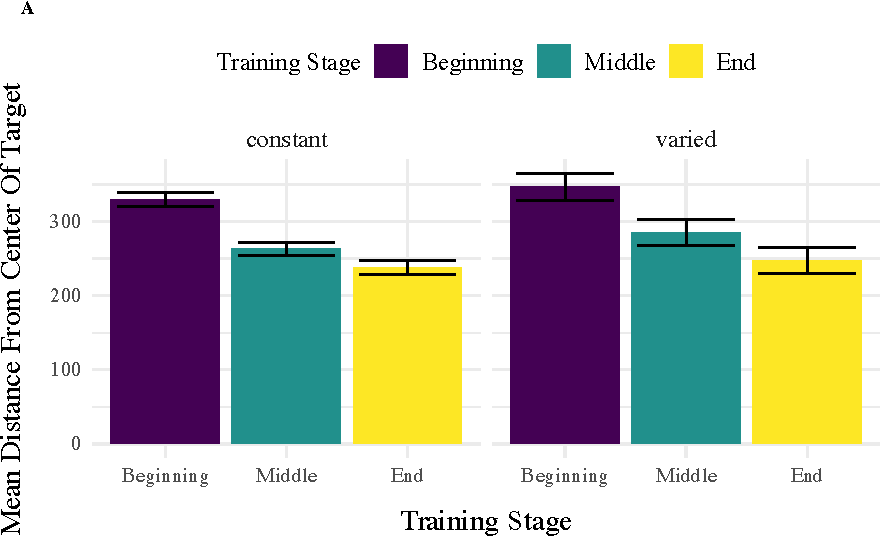
\includegraphics[keepaspectratio]{manuscript_files/figure-pdf/fig-e2train-1.pdf}}

}

\caption{\label{fig-e2train}Training performance for the six constant
conditions, and the varied condition, binned into three stages. On the
left side, the six constant groups are averaged together, as are the two
training positions for the varied group. On the right side, the six
constant groups are shown separately, with each set of bars representing
the beginning, middle, and end of training for a single constant group
that trained from the position indicated on the x-axis. Figure 5b also
shows training performance separately for both throwing locations
trained by the varied group. Error bars indicate standard error of the
mean.}

\end{figure}%

\paragraph{Testing Phase}\label{testing-phase-1}

In Experiment 2, a single varied condition (trained from two positions,
500 and 800), was compared against six separate constant groups (trained
from a single position, 400, 500, 625, 675, 800 or 900). For the testing
phase, all participants were tested from all six positions, four of
which were novel for the varied condition, and five of which were novel
for each of the constant groups. For a general comparison, we took the
absolute deviations for each throwing position and computed standardized
scores across all participants, and then averaged across throwing
position. The six constant groups were then collapsed together allowing
us to make a simple comparison between training conditions (constant
vs.~varied). A type III between-subjects ANOVA was performed, yielding a
significant effect of condition F(1,206)=4.33, p=.039, \(\eta^{2}_G\)
=.02. Descriptive statistics for each condition are shown in table 2. In
Figure~\ref{fig-e2testa} visualizes the consistent advantage of the
varied condition over the constant groups across the testing positions.
Figure~\ref{fig-e2testa} shows performance between the varied condition
and the individual constant groups.

\begin{figure}

\centering{

\pandocbounded{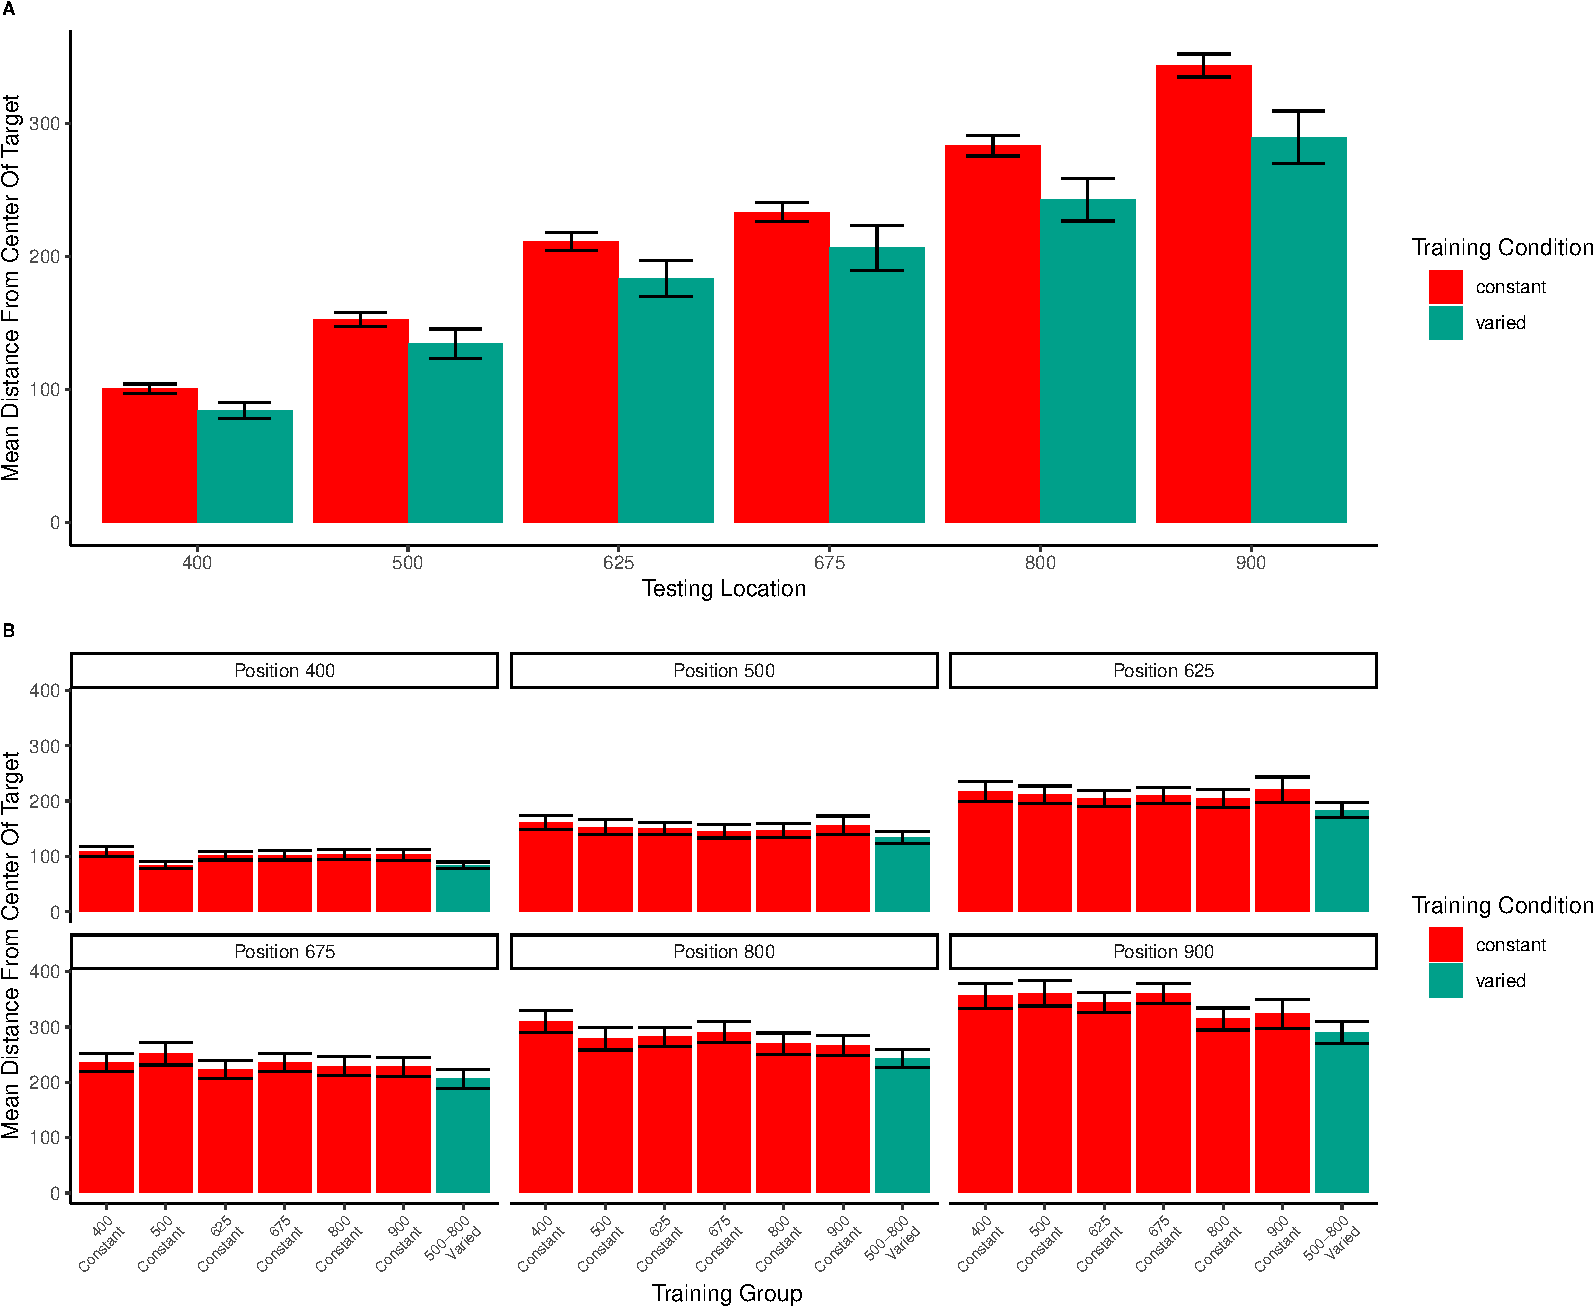
\includegraphics[keepaspectratio]{manuscript_files/figure-pdf/fig-e2testa-1.pdf}}

}

\caption{\label{fig-e2testa}Testing phase performance from each of the
six testing positions. The six constant conditions are averaged together
into a single constant group, compared against the single varied-trained
group.B) Transfer performance from each of the 6 throwing locations from
which all participants were tested. Each bar represents performance from
one of seven distinct training groups (six constant groups in red, one
varied group in blue). The x axis labels indicate the location(s) from
which each group trained. Lower values along the y axis reflect better
performance at the task (closer distance to target center). Error bars
indicate standard error of the mean.}

\end{figure}%

\hfill\break
\hfill\break
\hfill\break

\begin{longtable}[]{@{}lll@{}}

\caption{\label{tbl-e2table1}Transfer performance from each of the 6
throwing locations from which all participants were tested. Each bar
represents performance from one of seven distinct training groups (six
constant groups in red, one varied group in blue). The x axis labels
indicate the location(s) from which each group trained. Lower values
along the y axis reflect better performance at the task (closer distance
to target center). Error bars indicate standard error of the mean.}

\tabularnewline

\toprule\noalign{}
Position & Constant & Varied \\
\midrule\noalign{}
\endhead
\bottomrule\noalign{}
\endlastfoot
400 & 100.59(46.3) & 83.92(33.76) \\
500 & 152.28(69.82) & 134.38(61.38) \\
625 & 211.21(90.95) & 183.51(75.92) \\
675 & 233.32(93.35) & 206.32(94.64) \\
800 & 283.24(102.85) & 242.65(89.73) \\
900 & 343.51(114.33) & 289.62(110.07) \\

\end{longtable}

Next, we compared the testing performance of constant and varied groups
from only positions that participants had not encountered during
training. Constant participants each had 5 novel positions, whereas
varied participants tested from 4 novel positions (400,625,675,900). We
first standardized performance within in each position, and then
averaged across positions. Here again, we found a significant effect of
condition (constant vs.~varied): F(1,206)=4.30, p=.039, \(\eta^{2}_G\) =
.02 .

\begin{longtable}[]{@{}lll@{}}

\caption{\label{tbl-e2table2}Testing performance from novel positions.
Includes data only from positions that were not encountered during the
training stage (e.g., excludes positions 500 and 800 for the varied
group, and one of the six locations for each of the constant groups).
Table presents Mean absolute deviations from the center of the target,
and standard deviations in parenthesis.}

\tabularnewline

\toprule\noalign{}
Position & Constant & Varied \\
\midrule\noalign{}
\endhead
\bottomrule\noalign{}
\endlastfoot
400 & 98.84(45.31) & 83.92(33.76) \\
500 & 152.12(69.94) & NA \\
625 & 212.91(92.76) & 183.51(75.92) \\
675 & 232.9(95.53) & 206.32(94.64) \\
800 & 285.91(102.81) & NA \\
900 & 346.96(111.35) & 289.62(110.07) \\

\end{longtable}

Finally, corresponding to the comparison of position 760 from Experiment
1, we compared the test performance of the varied group against the
constant group from only the positions that the constant groups trained.
Such positions were novel to the varied group (thus this analysis
omitted two constant groups that trained from positions 500 or 800 as
those positions were not novel to the varied group).
Figure~\ref{fig-e2test1} displays the subset of comparisons utilized for
this analysis. Again, we standardized performance within each position
before performing the analyses on the aggregated data. In this case, the
effect of condition did not reach statistical significance
F(1,149)=3.14, p=.079, \(\eta^{2}_G\) = .02. Table 4 provides
descriptive statistics.

\begin{figure}

\centering{

\pandocbounded{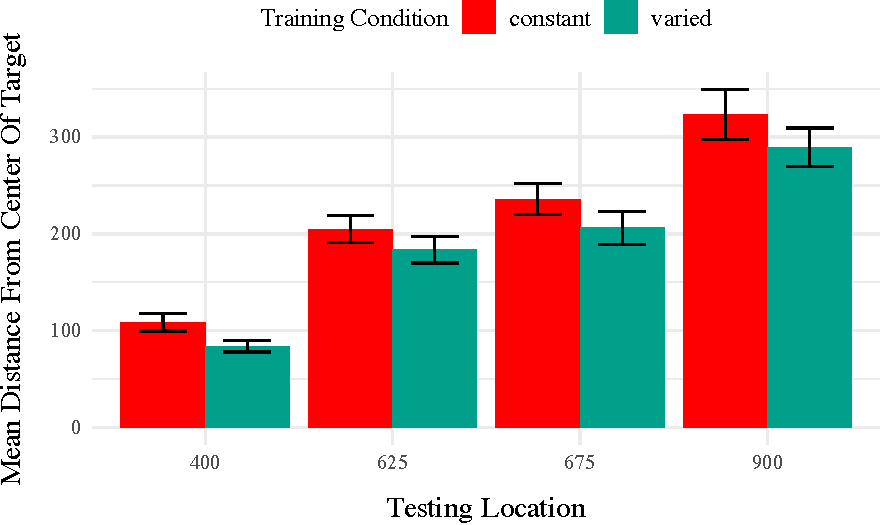
\includegraphics[keepaspectratio]{manuscript_files/figure-pdf/fig-e2test1-1.pdf}}

}

\caption{\label{fig-e2test1}A comparison of throwing location that are
identical to those trained by the constant participants (e.g., constant
participants trained at position 900, tested from position 900), which
are also novel to the varied-trained participants (thus excluding
positions 500 and 800). Error bars indicate standard error of the mean.}

\end{figure}%

\hfill\break
\hfill\break

\begin{longtable}[]{@{}lll@{}}

\caption{\label{tbl-e2tab3}Testing performance from the locations
trained by constant participants and novel to varied participants.
Locations 500 and 800 are not included as these were trained by the
varied participants. Table presents Mean absolute deviation from the
center of the target, and standard deviations in parenthesis.}

\tabularnewline

\toprule\noalign{}
Position & Constant & Varied \\
\midrule\noalign{}
\endhead
\bottomrule\noalign{}
\endlastfoot
400 & 108.85(50.63) & 83.92(33.76) \\
625 & 204.75(84.66) & 183.51(75.92) \\
675 & 235.75(81.15) & 206.32(94.64) \\
900 & 323.5(130.9) & 289.62(110.07) \\

\end{longtable}

\subsubsection{Experiment 2 Discussion}\label{experiment-2-discussion}

The results of Experiment 2 largely conform to the findings of
Experiment 1. Participants in both varied and constant conditions
improved at the task during the training phase. We did not observe the
common finding of training under varied conditions producing worse
performance during acquisition than training under constant conditions
(\citeproc{ref-catalanoDistantTransferCoincident1984a}{Catalano \&
Kleiner, 1984};
\citeproc{ref-wrisbergVariabilityPracticeHypothesis1987}{Wrisberg et
al., 1987}), which has been suggested to relate to the subsequent
benefits of varied training in retention and generalization testing
(\citeproc{ref-soderstromLearningPerformanceIntegrative2015}{Soderstrom
\& Bjork, 2015}). However, our finding of no difference in training
performance between constant and varied groups has been observed in
previous work (\citeproc{ref-chuaPracticeVariabilityPromotes2019}{Chua
et al., 2019};
\citeproc{ref-moxleySchemaVariabilityPractice1979}{Moxley, 1979};
\citeproc{ref-pigottMotorSchemaStructure1984}{Pigott \& Shapiro, 1984}).

In the testing phase, our varied group significantly outperformed the
constant conditions in both a general comparison, and in an analysis
limited to novel throwing positions. The observed benefit of varied over
constant training echoes the findings of many previous visuomotor skill
learning studies that have continued to emerge since the introduction of
Schmidt's influential Schema Theory
(\citeproc{ref-catalanoDistantTransferCoincident1984a}{Catalano \&
Kleiner, 1984}; \citeproc{ref-chuaPracticeVariabilityPromotes2019}{Chua
et al., 2019};
\citeproc{ref-goodwinEffectDifferentQuantities1998}{Goodwin et al.,
1998}; \citeproc{ref-mccrackenTestSchemaTheory1977}{McCracken \&
Stelmach, 1977};
\citeproc{ref-moxleySchemaVariabilityPractice1979}{Moxley, 1979};
\citeproc{ref-newellVariabilityPracticeTransfer1976}{Newell \& Shapiro,
1976}; \citeproc{ref-pigottMotorSchemaStructure1984}{Pigott \& Shapiro,
1984}; \citeproc{ref-rollerVariablePracticeLenses2001}{Roller et al.,
2001}; \citeproc{ref-schmidtSchemaTheoryDiscrete1975}{Schmidt, 1975};
\citeproc{ref-willeyLongtermMotorLearning2018}{Willey \& Liu, 2018b};
\citeproc{ref-wrisbergVariabilityPracticeHypothesis1987}{Wrisberg et
al., 1987}; \citeproc{ref-wulfEffectTypePractice1991}{Wulf, 1991}). We
also join a much smaller set of research to observe this pattern in a
computerized task (\citeproc{ref-seowTransferEffectsVaried2019}{Seow et
al., 2019}). One departure from the experiment 1 findings concerns the
pattern wherein the varied group outperformed the constant group even
from the training position of the constant group, which was significant
in experiment 1, but did not reach significance in experiment 2.
Although this pattern has been observed elsewhere in the literature
(\citeproc{ref-goodeSuperiorityVariableRepeated2008}{Goode et al.,
2008}; \citeproc{ref-kerrSpecificVariedPractice1978}{Kerr \& Booth,
1978}), the overall evidence for this effect appears to be far weaker
than for the more general benefit of varied training in conditions novel
to all training groups.

\subsection{Computational Model}\label{computational-model}

\emph{Controlling for the similarity between training and testing.} The
primary goal of Experiment 2 was to examine whether the benefits of
variability would persist after accounting for individual differences in
the similarity between trained and tested throwing locations. To this
end, we modelled each throw as a two-dimensional point in the space of x
and y velocities applied to the projectile at the moment of release. For
each participant, we took each individual training throw, and computed
the similarity between that throw and the entire population of throws
within the solution space for each of the 6 testing positions. We
defined the solution space empirically as the set of all combinations of
x and y throw velocities that resulted in hitting the target. We then
summed each of the trial-level similarities to produce a single
similarity for each testing position score relating how the participant
threw the ball during training and the solutions that would result in
target hits from each of the six testing positions -- thus resulting in
six separate similarity scores for each participant.
Figure~\ref{fig-taskSpace} visualizes the solution space for each
location and illustrates how different combinations of x and y velocity
result in successfully striking the target from different launching
positions. As illustrated in Figure~\ref{fig-taskSpace}, the solution
throws represent just a small fraction of the entire space of velocity
combinations used by participants throughout the experiment.

\begin{figure}

\centering{

\pandocbounded{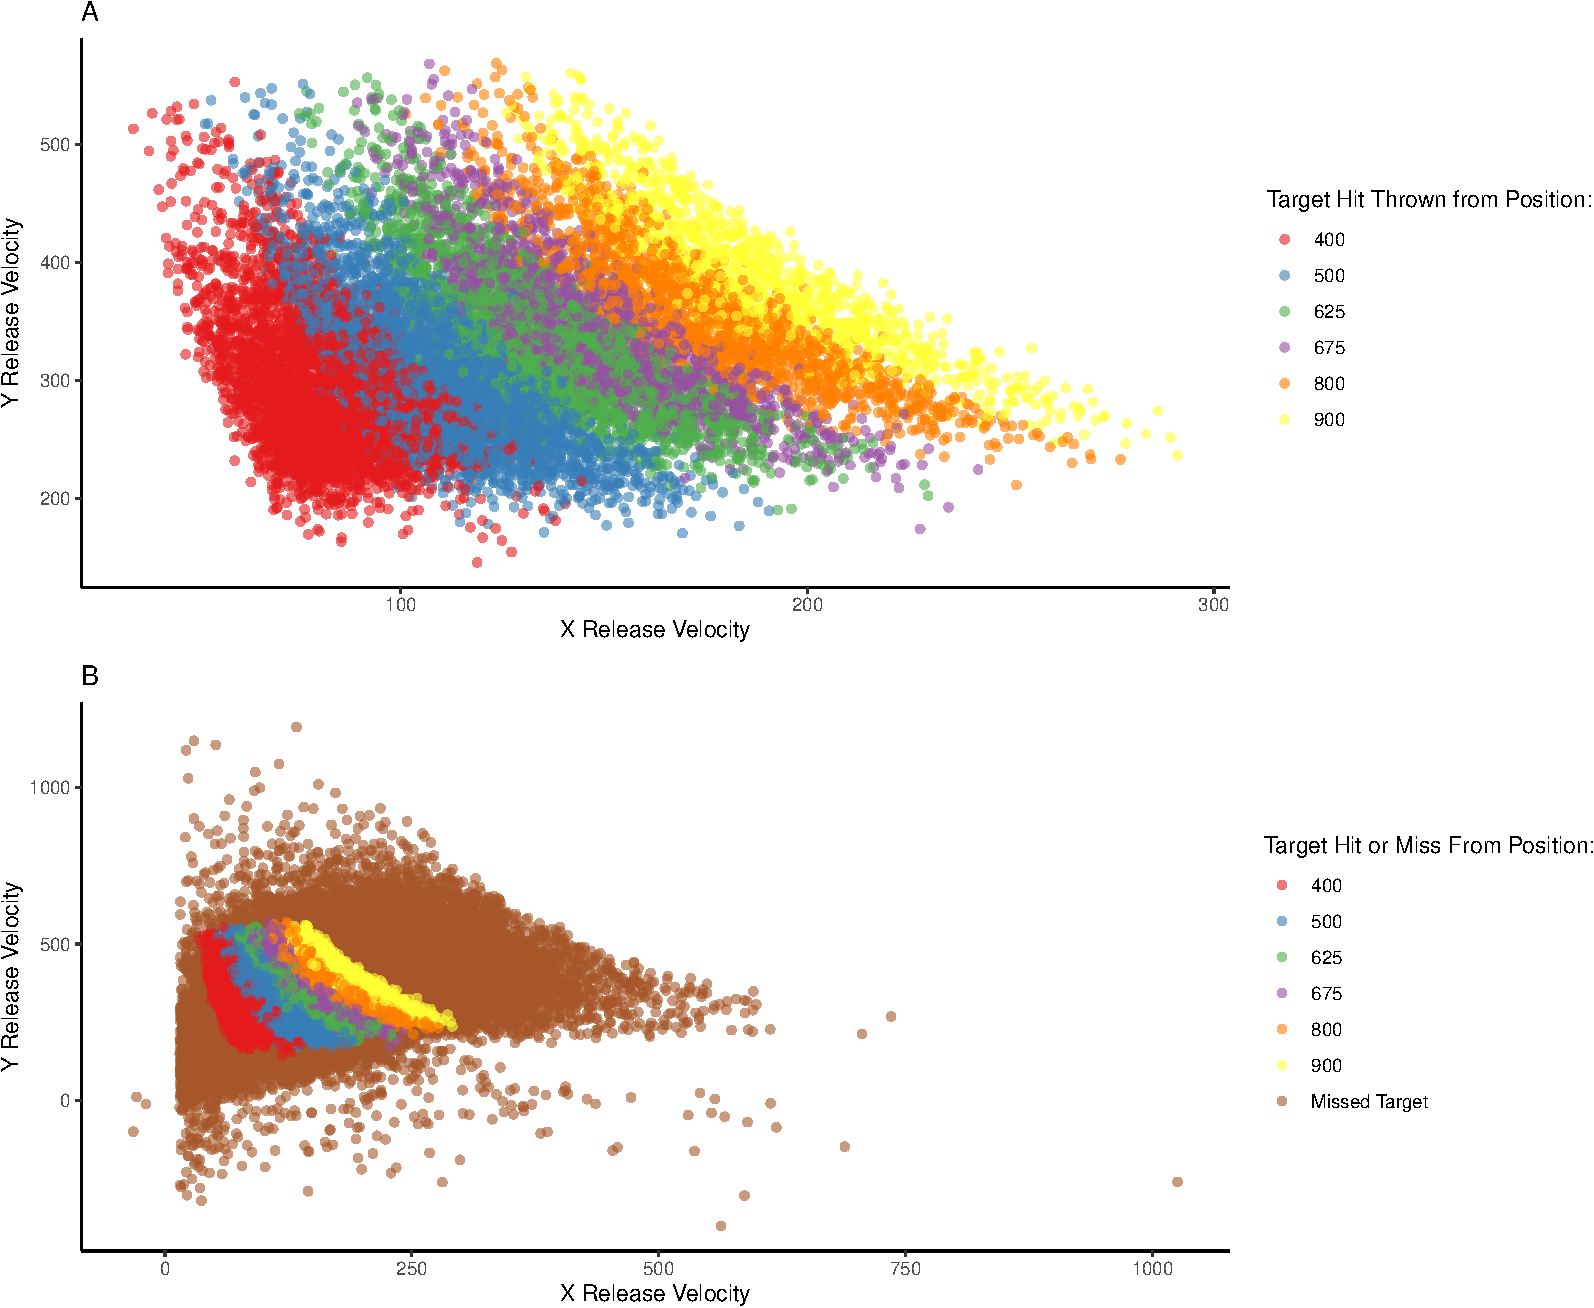
\includegraphics[keepaspectratio]{manuscript_files/figure-pdf/fig-taskSpace-1.pdf}}

}

\caption{\label{fig-taskSpace}A) A visual representation of the
combinations of throw parameters (x and y velocities applied to the ball
at launch), which resulted in target hits during the testing phase. This
empirical solution space was compiled from all of the participants in
Experiment 2. B) shows the solution space within the context of all of
the throws made throughout the testing phase of the experiment.}

\end{figure}%

For each individual trial, the Euclidean distance (Equation 1) was
computed between the velocity components (x and y) of that trial and the
velocity components of each individual solution throw for each of the 6
positions from which participants would be tested in the final phase of
the study. The P parameter in Equation 1 is set equal to 2, reflecting a
Gaussian similarity gradient. Then, as per an instance-based model of
similarity (\citeproc{ref-loganInstanceTheoryAttention2002a}{Logan,
2002}; \citeproc{ref-nosofskySimilarityScalingCognitive1992}{Nosofsky,
1992}), these distances were multiplied by a sensitivity parameter, c,
and then exponentiated to yield a similarity value. The parameter c
controls the rate with which similarity-based generalization drops off
as the Euclidean distance between two throws in x- and y-velocity space
increases. If c has a large value, then even a small difference between
two throws' velocities greatly decreases the extent of generalization
from one to the other. A small value for c produces broad generalization
from one throw to another despite relatively large differences in their
velocities. The similarity values for each training individual throw
made by a given participant were then summed to yield a final similarity
score, with a separate score computed for each of the 6 testing
positions. The final similarity score is construable as index of how
accurate the throws a participant made during the training phase would
be for each of the testing positions.

\textbf{Equation 1:}
\[ Similarity_{I,J} = \sum_{i=I}\sum_{j=J} (e^{-c^\cdot d^{p}_{i,j}}) \]

\textbf{Equation 2:}
\[ d_{i,j} = \sqrt{(x_{Train_i}-x_{Solution_j})^2 + (y_{Train_i}-y_{Solution_j})^2 } \]

A simple linear regression revealed that these similarity scores were
significantly predictive of performance in the transfer stage, t
=-15.88, p\textless.01, \(r^2\)=.17, such that greater similarity
between training throws and solution spaces for each of the test
locations resulted in better performance. We then repeated the group
comparisons above while including similarity as a covariate in the
model. Comparing the varied and constant groups in testing performance
from all testing positions yielded a significant effect of similarity,
F(1, 205)=85.66, p\textless.001, \(\eta^{2}_G\) =.29, and also a
significant effect of condition (varied vs.~constant), F(1, 205)=6.03,
p=.015, \(\eta^{2}_G\) =.03. The group comparison limited to only novel
locations for the varied group pit against trained location for the
constant group resulted in a significant effect of similarity,
F(1,148)=31.12, p\textless.001, \(\eta^{2}_G\) =.18 as well as for
condition F(1,148)=11.55, p\textless.001, \(\eta^{2}_G\) =.07. For all
comparisons, the pattern of results was consistent with the initial
findings from Experiment 2, with the varied group still performing
significantly better than the constant group.

\subsubsection{Fitting model parameters separately by
group}\label{fitting-model-parameters-separately-by-group}

To directly control for similarity in Experiment 2, we developed a
model-based measure of the similarity between training throws and
testing conditions. This similarity measure was a significant predictor
of testing performance, e.g., participants whose training throws were
more similar to throws that resulted in target hits from the testing
positions, tended to perform better during the testing phase.
Importantly, the similarity measure did not explain away the group-level
benefits of varied training, which remained significant in our linear
model predicting testing performance after similarity was added to the
model. However, previous research has suggested that participants may
differ in their level of generalization as a function of prior
experience, and that such differences in generalization gradients can be
captured by fitting the generalization parameter of an instance-based
model separately to each group
(\citeproc{ref-hahnEffectsCategoryDiversity2005}{Hahn et al., 2005};
\citeproc{ref-lambertsFlexibleTuningSimilarity1994}{Lamberts, 1994}).
Relatedly, the influential Bayesian generalization model developed by
Tenenbaum \& Griffiths
(\citeproc{ref-tenenbaumGeneralizationSimilarityBayesian2001a}{2001})
predicts that the breadth of generalization will increase when a
rational agent encounters a wider variety of examples. Following these
leads, we assume that in addition to learning the task itself,
participants are also adjusting how generalizable their experience
should be. Varied versus constant participants may be expected to learn
to generalize their experience to different degrees. To accommodate this
difference, the generalization parameter of the instance-based model (in
the present case, the \(c\) parameter) can be allowed to vary between
the two groups to reflect the tendency of learners to adaptively tune
the extent of their generalization. One specific hypothesis is that
people adaptively set a value of c to fit the variability of their
training experience
(\citeproc{ref-nosofskyExemplarbasedAccountsMultiplesystem2000}{Nosofsky
\& Johansen, 2000};
\citeproc{ref-sakamotoTrackingVariabilityLearning2006}{Sakamoto et al.,
2006}). If one's training experience is relatively variable, as with the
variable training condition, then one might infer that future test
situations will also be variable, in which case a low value of c will
allow better generalization because generalization will drop off slowly
with training-to-testing distance. Conversely, if one's training
experience has little variability, as found in the constant training
conditions, then one might adopt a high value of \(c\) so that
generalization falls off rapidly away from the trained positions.

To address this possibility, we compared the original instance-based
model of similarity fit against a modified model which separately fits
the generalization parameter, \(c\), to varied and constant
participants. To perform this parameter fitting, we used the optim
function in R, and fit the model to find the \(c\) value(s) that
maximized the correlation between similarity and testing performance.

Both models generate distinct similarity values between training and
testing locations. Much like the analyses in Experiment 2, these
similarity values are regressed against testing performance in models of
the form shown below. As was the case previously, testing performance is
defined as the mean absolute distance from the center of the target
(with a separate score for each participant, from each position).

Linear models 1 and 3 both show that similarity is a significant
predictor of testing performance (p\textless.01). Of greater interest is
the difference between linear model 2, in which similarity is computed
from a single \(c\) value fit from all participants (Similarity1c), with
linear model 4, which fits the \(c\) parameter separately between groups
(Similarity2c). In linear model 2, the effect of training group remains
significant when controlling for Similarity1c (p\textless.01), with the
varied group still performing significantly better. However, in linear
model 4 the addition of the Similarity2c predictor results in the effect
of training group becoming nonsignificant (p=.40), suggesting that the
effect of varied vs.~constant training is accounted for by the
Similarity2c predictor. Next, to further establish a difference between
the models, we performed nested model comparisons using ANOVA, to see if
the addition of the training group parameter led to a significant
improvement in model performance. In the first comparison, ANOVA(Linear
Model 1, Linear Model 2), the addition of the training group predictor
significantly improved the performance of the model (F=22.07,
p\textless.01). However, in the second model comparison, ANOVA (Linear
model 3, Linear Model 4) found no improvement in model performance with
the addition of the training group predictor (F=1.61, p=.20).

Finally, we sought to confirm that similarity values generated from the
adjusted Similarity2c model had more predictive power than those
generated from the original Similarity1c model. Using the BIC function
in R, we compared BIC values between linear model 1 (BIC=14604.00) and
linear model 3 (BIC = 14587.64). The lower BIC value of model 3 suggests
a modest advantage for predicting performance using a similarity measure
computed with two \(c\) values over similarity computed with a single
\(c\) value. When fit with separate \(c\) values, the best fitting \(c\)
parameters for the model consistently optimized such that the \(c\)
value for the varied group (c=.00008) was smaller in magnitude than the
\(c\) value for the constant group (c= .00011). Recall that similarity
decreases as a Gaussian function of distance (equation 1 above), and a
smaller value of \(c\) will result in a more gradual drop-off in
similarity as the distance between training throws and testing solutions
increases.

In summary, our modeling suggests that an instance-based model which
assumes equivalent generalization gradients between constant and varied
trained participants is unable to account for the extent of benefits of
varied over constant training observed at testing. The evidence for this
in the comparative model fits is that when a varied/constant dummy-coded
variable for condition is explicitly added to the model, the variable
adds a significant contribution to the prediction of test performance,
with the variable condition yielding better performance than the
constant conditions. However, if the instance-based generalization model
is modified to assume that the training groups can differ in the
steepness of their generalization gradient, by incorporating a separate
generalization parameter for each group, then the instance-based model
can account for our experimental results without explicitly taking
training group into account. Henceforth this model will be referred to
as the Instance-based Generalization with Adaptive Similarity (IGAS)
model.

\subsection{Project 1 General
Discussion}\label{project-1-general-discussion}

Across two experiments, we found evidence in support of the benefits of
variability hypothesis in a simple, computerized projectile throwing
task. Generalization was observed in both constant and varied
participants, in that both groups tended to perform better at novel
positions in the testing phase than did participants who started with
those positions in the training phase. However, varied trained
participants consistently performed better than constant trained
participants, in terms of both the testing phase in general, and in a
comparison that only included untrained positions. We also found some
evidence for the less commonly observed pattern wherein varied-trained
participants outperform constant-trained participants even from
conditions identical to the constant group training
(\citeproc{ref-goodeSuperiorityVariableRepeated2008}{Goode et al.,
2008}; \citeproc{ref-greenPracticeVariabilityTransfer1995a}{Green et
al., 1995}; \citeproc{ref-kerrSpecificVariedPractice1978}{Kerr \& Booth,
1978}). In Experiment 1 varied participants performed significantly
better on this identity comparison. In Experiment 2, the comparison was
not significant initially, but became significant after controlling for
the similarity measure that incorporates only a single value for the
steepness of similarity-based generalization (\(c\)). Furthermore, we
showed that the general pattern of results from Experiment 2 could be
parsimoniously accommodated by an instance-based similarity model, but
only with the assumption that constant and varied participants
generalize their training experience to different degrees.

Our results thus suggest that the benefits of variation cannot be
explained by the varied-trained participants simply covering a broader
range of the task space. Rather, the modeling suggests that varied
participants also learn to adaptively tune their generalization function
such that throwing locations generalize more broadly to one another than
they do in the constant condition. A learning system could end up
adopting a higher \(c\) value in the constant than variable training
conditions by monitoring the trial-by-trial variability of the training
items. The \(c\) parameter would be adapted downwards when adjacent
training items are dissimilar to each other and adapted upwards when
adjacent training items are the same. In this fashion, contextually
appropriate \(c\) values could be empirically learned. This learning
procedure would capture the insight that if a situation has a high
amount variability, then the learner should be predisposed toward
thinking that subsequent test items will also show considerable
variability, in which case generalization gradients should be broad, as
is achieved by low values for \(c\). Sakamoto et al.
(\citeproc{ref-sakamotoTrackingVariabilityLearning2006}{2006})
implemented a similar learning mechanism for updating the generalization
paramater in an exemplar-based model (although in their model, a
separate generalization parameter is assigned to each exemplar). In
their experiment, participants were trained on a high variability and a
low variability category, and the dynamically updated generalization
parameter was necessary to account for broader generalization observed
around the high variability category when participants were tested with
an ambiguous intermediary item. In a subsequent work
(\citeproc{ref-sakamotoPuttingPsychologyBack2008}{Sakamoto et al.,
2008}), the same authors showed that a similar learning mechanism could
account for the pattern wherein participants generalize more broadly
around a category when the average distance between the category
exemplars is larger (however the only model tested in this work was a
prototype model).

Also of interest is whether the IGAS model can predict the pattern of
results wherein the varied condition outperforms the constant condition
even from the position on which the constant condition trained. Although
our models were fit using all of the Experiment 2 training and testing
data, not just that of the identity comparisons, in
Figure~\ref{fig-Toy-Model-dis} we demonstrate how a simplified version
of the IGAS model could in principle produce such a pattern. In addition
to the assumption of differential generalization between varied and
constant conditions, our simplified model makes explicit an assumption
that is incorporated into the full IGAS model -- namely that even when
being tested from a position identical to that which was trained, there
are always some psychological contextual differences between training
and testing throws, resulting in a non-zero dissimilarity.

\begin{figure}

\centering{

\pandocbounded{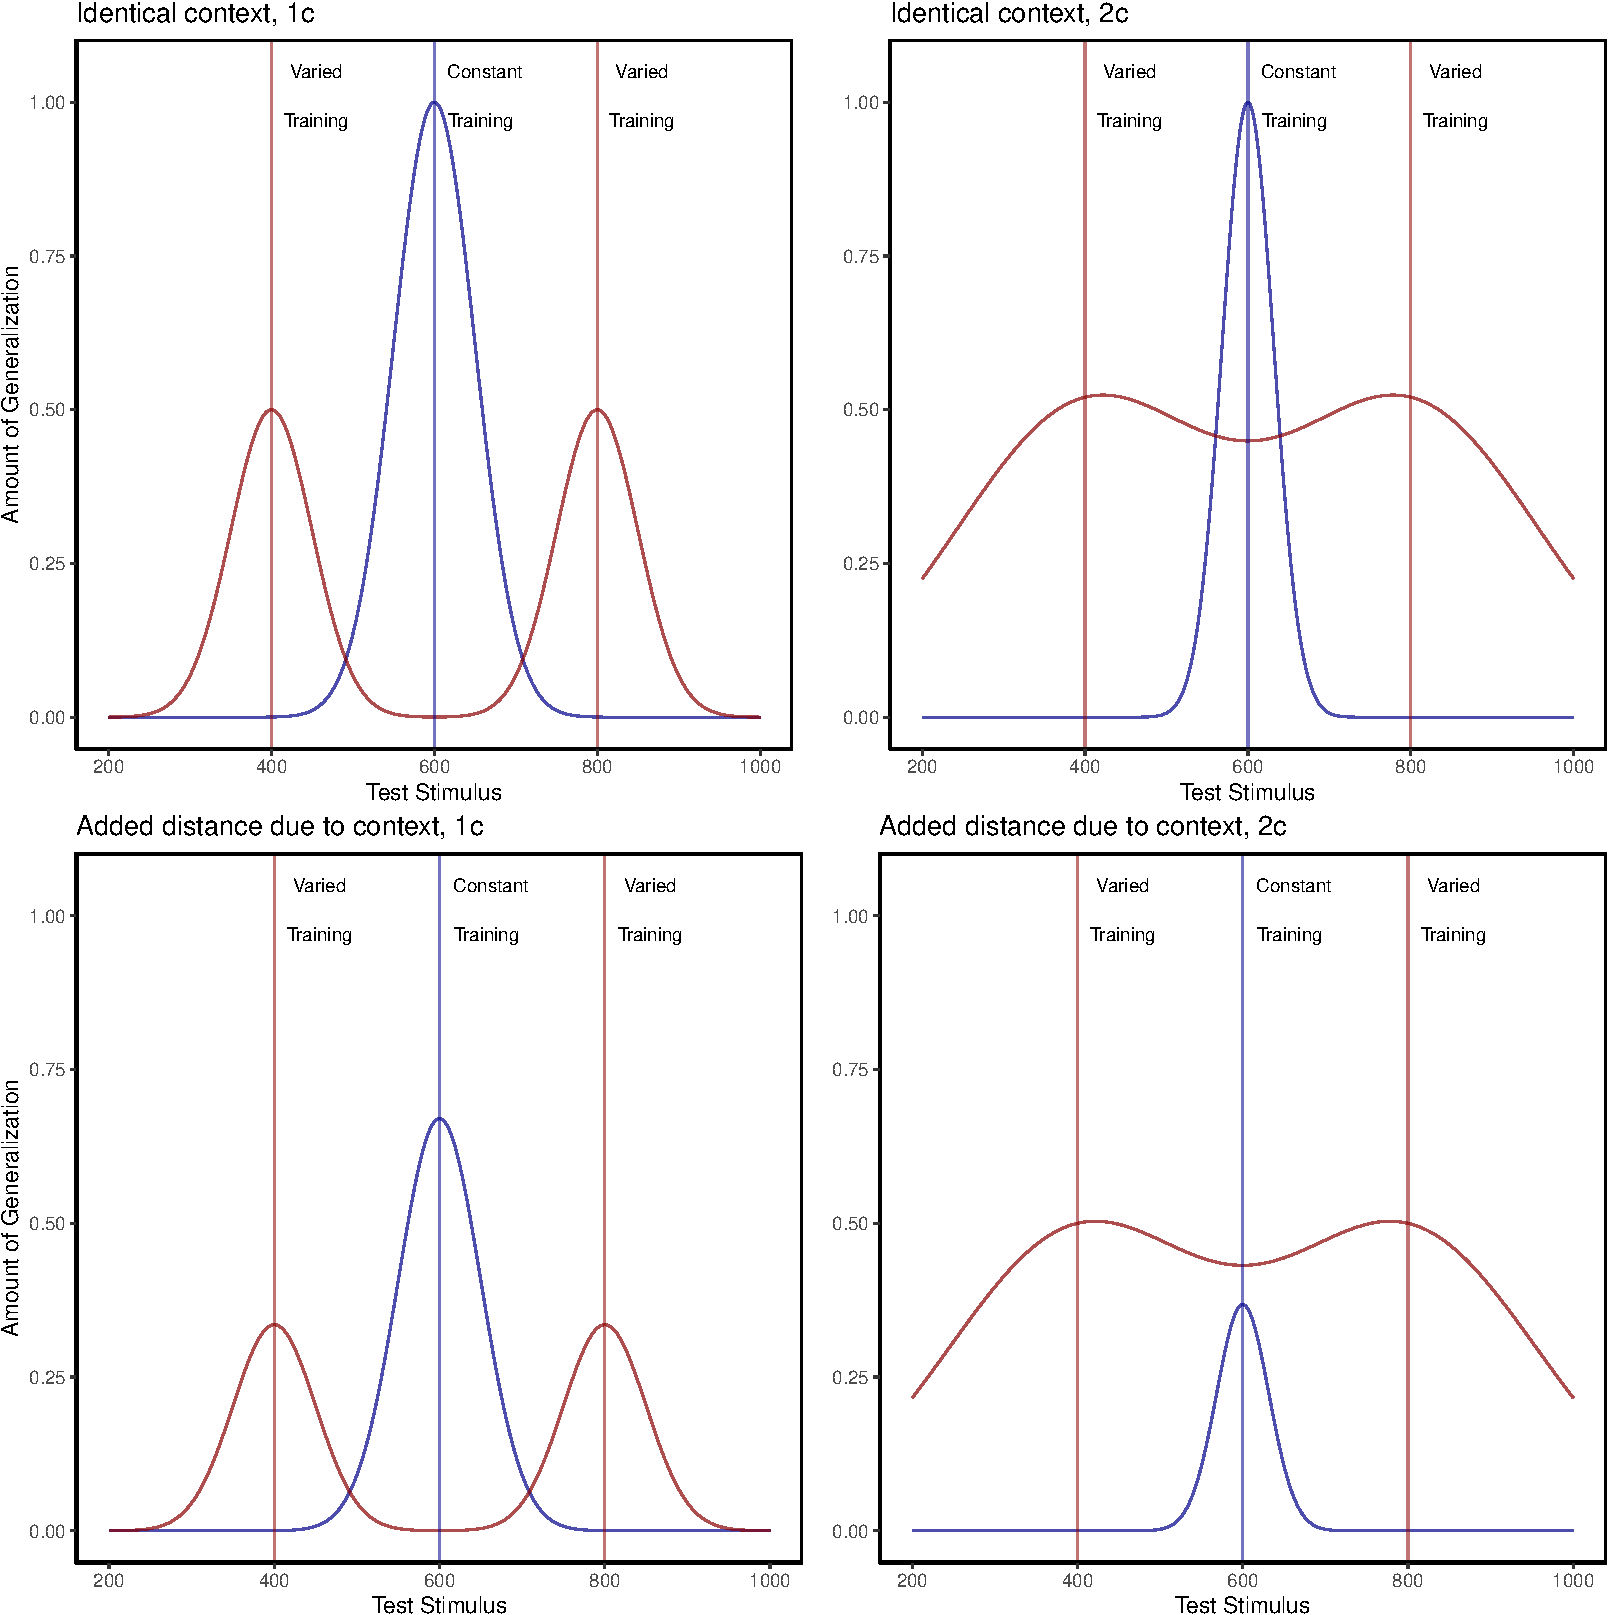
\includegraphics[keepaspectratio]{manuscript_files/figure-pdf/fig-Toy-Model-dis-1.pdf}}

}

\caption{\label{fig-Toy-Model-dis}A simple model depicting the necessity
of both of two separately fit generalization parameters, c, and a
positive distance between training and testing contexts, in order for an
instance model to predict a pattern of varied training from stimuli 400
and 800 outperforming constant training from position 600 at a test
position of 600. For the top left panel, in which the generalization
model assumes a single c value (-.008) for both varied and constant
conditions, and identical contexts across training and testing, the
equation which generates the varied condition is - Amount of
Generalization = \(e^{(c\cdot|x-800|)} + e^{(c\cdot|x-400|)}\), whereas
the constant group generalization is generated from
\(2\cdot e^{(c\cdot|x-600|)}\). For the top right panel, the c constants
in the original equations are different for the 2 conditions, with
\(c=-.002\) for the varied condition, and \(c=-.008\) for the constant
condition. The bottom two panels are generated from identical equations
to those immediately above, except for the addition of extra distance
(100 units) to reflect the assumption of some change in context between
training and testing conditions. Thus, the generalization model for the
varied condition in the bottom-right panel is of the form - Amount of
Generalization =
\(e^{(c_{varied}\cdot|x-800|)}+e^{(c_{varied}\cdot|x-400|)}\) .}

\end{figure}%

As described above, the idea that learners flexibly adjust their
generalization gradient based on prior experience does have precedent in
the domains of category learning
(\citeproc{ref-ahaConceptLearningFlexible1992}{Aha \& Goldstone, 1992};
\citeproc{ref-briscoeConceptualComplexityBias2011}{Briscoe \& Feldman,
2011}; \citeproc{ref-hahnEffectsCategoryDiversity2005}{Hahn et al.,
2005}; \citeproc{ref-lambertsFlexibleTuningSimilarity1994}{Lamberts,
1994}; \citeproc{ref-opdebeeckRepresentationPerceivedShape2008}{Op de
Beeck et al., 2008}), and sensorimotor adaptation
(\citeproc{ref-marongelliAdvantageFlexibleNeuronal2013}{Marongelli \&
Thoroughman, 2013};
\citeproc{ref-taylorContextdependentGeneralization2013}{Taylor \& Ivry,
2013}; \citeproc{ref-thoroughmanRapidReshapingHuman2005}{Thoroughman \&
Taylor, 2005}). Lamberts
(\citeproc{ref-lambertsFlexibleTuningSimilarity1994}{1994}) showed that
a simple manipulation of background knowledge during a categorization
test resulted in participants generalizing their training experience
more or less broadly, and moreover that such a pattern could be captured
by allowing the generalization parameter of an instance-based similarity
model to be fit separately between conditions. The flexible
generalization parameter has also successfully accounted for
generalization behavior in cases where participants have been trained on
categories that differ in their relative variability
(\citeproc{ref-hahnEffectsCategoryDiversity2005}{Hahn et al., 2005};
\citeproc{ref-sakamotoTrackingVariabilityLearning2006}{Sakamoto et al.,
2006}). However, to the best of our knowledge, IGAS is the first
instance-based similarity model that has been put forward to account for
the effect of varied training in a visuomotor skill task. Although IGAS
was inspired by work in the domain of category learning, its success in
a distinct domain may not be surprising in light of the numerous prior
observations that at least certain aspects of learning and
generalization may operate under common principles across different
tasks and domains (\citeproc{ref-censorCommonMechanismsHuman2012}{Censor
et al., 2012}; \citeproc{ref-hillsCentralExecutiveSearch2010}{Hills et
al., 2010};
\citeproc{ref-jamiesonInstanceTheoryDomaingeneral2022}{Jamieson et al.,
2022}; \citeproc{ref-lawSharedMechanismsPerceptual2010}{Law \& Gold,
2010}; \citeproc{ref-roarkComparingPerceptualCategory2021}{Roark et al.,
2021};
\citeproc{ref-rosenbaumAcquisitionIntellectualPerceptualMotor2001}{Rosenbaum
et al., 2001}; \citeproc{ref-vigoLearningDifficultyVisual2018}{Vigo et
al., 2018};
\citeproc{ref-wallIdentifyingRelationshipsCognitive2021}{Wall et al.,
2021}; \citeproc{ref-wuSimilaritiesDifferencesSpatial2020}{Wu et al.,
2020}; \citeproc{ref-yangGeneralLearningAbility2020}{J. Yang et al.,
2020}).

Our modelling approach does differ from category learning
implementations of instance-based models in several ways. One such
difference is the nature of the training instances that are assumed to
be stored. In category learning studies, instances are represented as
points in a multidimensional space of all of the attributes that define
a category item (e.g., size/color/shape). Rather than defining instances
in terms of what stimuli learners experience, our approach assumes that
stored, motor instances reflect how they act, in terms of the velocity
applied to the ball on each throw. An advantage of many motor learning
tasks is the relative ease with which task execution variables can be
directly measured (e.g., movement force, velocity, angle, posture) in
addition to the decision and response time measures that typically
exhaust the data generated from more classical cognitive tasks. Of
course, whether learners actually are storing each individual motor
instance is a fundamental question beyond the scope of the current work
-- though as described in the introduction there is some evidence in
support of this idea
(\citeproc{ref-chamberlinNoteSchemaExemplar1992}{Chamberlin \& Magill,
1992a}; \citeproc{ref-crumpEpisodicContributionsSequential2010}{Crump \&
Logan, 2010}; \citeproc{ref-hommelEventFilesEvidence1998}{Hommel, 1998};
\citeproc{ref-meighWhatMemoryRepresentation2018}{Meigh et al., 2018};
\citeproc{ref-poldrackRelationshipSkillLearning1999}{Poldrack et al.,
1999}). A particularly noteworthy instance-based model of sensory-motor
behavior is the Knowledge II model of Rosenbaum and colleagues
(\citeproc{ref-cohenWhereGraspsAre2004}{R. G. Cohen \& Rosenbaum, 2004};
\citeproc{ref-rosenbaumPlanningReachesEvaluating1995}{Rosenbaum et al.,
1995}). Knowledge II explicitly defines instances as postures (joint
combinations), and is thus far more detailed than IGAS in regards to the
contents of stored instances. Knowledge II also differs from IGAS in
that learning is accounted for by both the retrieval of stored postures,
and the generation of novel postures via the modification of retrieved
postures. A promising avenue for future research would be to combine the
adaptive similarity mechanism of IGAS with the novel instance generation
mechanisms of Knowledge II.

Our findings also have some conceptual overlap with an earlier study on
the effects of varied training in a coincident timing task
(\citeproc{ref-catalanoDistantTransferCoincident1984a}{Catalano \&
Kleiner, 1984}). In this task, participants observe a series of lamps
lighting up consecutively, and attempt to time a button press with the
onset of the final lamp. The design consisted of four separate constant
groups, each training from a single lighting velocity, and a single
varied group training with all four of the lighting velocities used by
the individual constant groups. Participants were then split into four
separate testing conditions, each of which were tested from a single
novel lighting velocity of varying distance from the training
conditions. The result of primary interest was that all participants
performed worse as the distance between training and testing velocity
increased -- a typical generalization decrement. However, varied
participants showed less of a decrement than did constant participants.
The authors take this result as evidence that varied training results in
a less-steep generalization gradient than does constant training.
Although the experimental conclusions of Catalano and Kleiner are
similar to our own, our work is novel in that we account for our results
with a cognitive model, and without assuming the formation of a schema.
Additionally, the way in which Catalano and Kleiner collapse their
separate constant groups together may result in similarity confounds
between varied and constant conditions that leaves their study open to
methodological criticisms, especially in light of related work which
demonstrated that the extent to which varied training may be beneficial
can depend on whether the constant group they are compared against
trained from similar conditions to those later tested
(\citeproc{ref-wrisbergVariabilityPracticeHypothesis1987}{Wrisberg et
al., 1987}). Our study alleviates such concerns by explicitly
controlling for similarity.

\subsubsection{Limitations}\label{limitations}

A limitation of this study concerns the ordering of the testing/transfer
trials at the conclusion of both experiments. Participants were tested
from each separate position (4 in Experiment 1, 6 in Experiment 2) in a
random, intermixed order. Because the varied group was trained from two
positions that were also randomly ordered, they may have benefited from
experience with this type of sequencing, whereas the constant groups had
no experience with switching between positions trial to trial. This
concern is somewhat ameliorated by the fact that the testing phase
performance of the constant groups from their trained position was not
significantly worse than their level of performance at the end of the
training phase, suggesting that they were not harmed by random ordering
of positions during testing. It should also be noted that the
computerized task utilized in the present work is relatively simple
compared to many of the real-world tasks utilized in prior research. It
is thus conceivable that the effect of variability in more complex tasks
is distinct from the process put forward in the present work. An
important challenge for future work will be to assess the extent to
which IGAS can account for generalization in relatively complex tasks
with far more degrees of freedom.

It is common for psychological process models of categorization learning
to use an approach such as multidimensional scaling so as to transform
the stimuli from the physical dimensions used in the particular task
into the psychological dimensions more reflective of the actual human
representations
(\citeproc{ref-nosofskySimilarityScalingCognitive1992}{Nosofsky, 1992};
\citeproc{ref-shepardUniversalLawGeneralization1987}{Shepard, 1987}).
Such scaling typically entails having participants rate the similarity
between individual items and using these similarity judgements to then
compute the psychological distances between stimuli, which can then be
fed into a subsequent model. In the present investigation, there was no
such way to scale the x and y velocity components in terms of the
psychological similarity, and thus our modelling does rely on the
assumption that the psychological distances between the different
throwing positions are proportional to absolute distances in the metric
space of the task (e.g., the relative distance between positions 400 and
500 is equivalent to that between 800 and 900). However, an advantage of
our approach is that we are measuring similarity in terms of how
participants behave (applying a velocity to the ball), rather than the
metric features of the task stimuli.

\subsubsection{Conclusion}\label{conclusion}

Our experiments demonstrate a reliable benefit of varied training in a
simple projectile launching task. Such results were accounted for by an
instance-based model that assumes that varied training results in the
computation of a broader similarity-based generalization gradient.
Instance-based models augmented with this assumption may be a valuable
approach towards better understanding skill generalization and transfer.

\newpage{}

\section{Project 2}\label{project-2}

\subsection{Introduction}\label{introduction-2}

A longstanding issue across both science and instruction has been to
understand how various aspects of an educational curriculum or training
program influence learning acquisition and generalization. One such
aspect, which has received a great deal of research attention, is the
variability of examples experienced during training
(\citeproc{ref-ravivHowVariabilityShapes2022}{Raviv et al., 2022}). The
influence of training variation has been studied in numerous domains,
including category learning
(\citeproc{ref-cohenCategoryVariabilityExemplar2001}{A. L. Cohen et al.,
2001}; \citeproc{ref-posnerGenesisAbstractIdeas1968}{Posner \& Keele,
1968}), visuomotor learning
(\citeproc{ref-bernikerEffectsTrainingBreadth2014}{Berniker et al.,
2014}; \citeproc{ref-schmidtSchemaTheoryDiscrete1975}{Schmidt, 1975}),
language learning (\citeproc{ref-perryLearnLocallyThink2010}{Perry et
al., 2010}), and education
(\citeproc{ref-braithwaiteEffectsVariationPrior2015}{Braithwaite \&
Goldstone, 2015}; \citeproc{ref-guoEffectsExampleVariability2014}{Guo et
al., 2014}). The pattern of results is complex, with numerous studies
finding both beneficial
(\citeproc{ref-braunMotorTaskVariation2009}{Braun et al., 2009};
\citeproc{ref-catalanoDistantTransferCoincident1984a}{Catalano \&
Kleiner, 1984};
\citeproc{ref-gormanInstancebasedModelAccount2022}{Gorman \& Goldstone,
2022}; \citeproc{ref-rollerVariablePracticeLenses2001}{Roller et al.,
2001}), as well as null or negative effects
(\citeproc{ref-brekelmansDoesHighVariability2022}{Brekelmans et al.,
2022}; \citeproc{ref-huHighvariabilityTrainingDoes2024}{Hu \& Nosofsky,
2024}; \citeproc{ref-vanrossumSchmidtSchemaTheory1990}{Van Rossum,
1990}). The present study seeks to contribute to the large body of
existing research by examining the influence of variability in
visuomotor function learning - a domain in which it has been relatively
under-studied.

\subsubsection{Function Learning and
Extrapolation}\label{function-learning-and-extrapolation}

The study of human function learning investigates how people learn
relationships between continuous input and output values. Function
learning is studied both in tasks where individuals are exposed to a
sequence of input/output pairs
(\citeproc{ref-deloshExtrapolationSineQua1997}{DeLosh et al., 1997};
\citeproc{ref-mcdanielEffectsSpacedMassed2013}{McDaniel et al., 2013}),
or situations where observers are presented with an incomplete
scatterplot or line graph and make predictions about regions of the plot
that do not contain data
(\citeproc{ref-ciccioneCanHumansPerform2021}{Ciccione \& Dehaene, 2021};
\citeproc{ref-courrieuQuickApproximationBivariate2012}{Courrieu, 2012};
\citeproc{ref-saidExtrapolationAccuracyUnderestimates2021}{Said \&
Fischer, 2021};
\citeproc{ref-schulzCommunicatingCompositionalPatterns2020}{Schulz et
al., 2020}). Studies of function learning often compare the difficulty
of learning functions of different underlying forms (e.g.~linear,
bi-linear, power, sinusoidal), and the extent to which participants can
accurately respond to novel inputs that fall in-between previously
experienced inputs (interpolation testing), or that fall outside the
range of previously experienced inputs (extrapolation).

Carroll (\citeproc{ref-carrollFunctionalLearningLearning1963}{1963})
conducted the earliest work on function learning. Input stimuli and
output responses were both lines of varying length. The correct output
response was related to the length of the input line by a linear,
quadratic, or random function. Participants in the linear and quadratic
performed above chance levels during extrapolation testing, with those
in the linear condition performing the best overall. Carroll argued that
these results were best explained by a rule-based model wherein learners
form an abstract representation of the underlying function. Subsequent
work by Brehmer
(\citeproc{ref-brehmerHypothesesRelationsScaled1974}{1974}), testing a
wider array of functional forms, provided further evidence for superior
extrapolation in tasks with linear functions. Brehmer argued that
individuals start out assuming a linear function, but given sufficient
error will progressively test alternative hypotheses with polynomials of
greater degree. Koh \& Meyer
(\citeproc{ref-kohFunctionLearningInduction1991}{1991}) employed a
visuomotor function learning task, wherein participants were trained on
examples from an unknown function relating the length of an input line
to the duration of a response (time between keystrokes). In this domain,
participants performed best when the relation between line length and
response duration was determined by a power law, as opposed to linear
function. Koh and Meyer developed the log-polynomial adaptive-regression
model to account for their results.

The first significant challenge to rule-based accounts of function
learning was put forth by DeLosh et al.
(\citeproc{ref-deloshExtrapolationSineQua1997}{1997}) . In their task,
participants learned to associate stimulus magnitudes with response
magnitudes that were related via either linear, exponential, or
quadratic function. Participants approached ceiling performance by the
end of training in each function condition, and were able to accurately
respond on interpolation testing trials. All three conditions
demonstrated some capacity for extrapolation, however participants in
the linear condition tended to underestimate the true function, while
exponential and quadratic participants reliably overestimated the true
function on extrapolation trials. Extrapolation and interpolation
performances are depicted in Figure~\ref{fig-delosh-extrap}.

The authors evaluated the rule-based models introduced in earlier
research (with some modifications enabling trial-by-trial learning). The
polynomial hypothesis testing model
(\citeproc{ref-brehmerHypothesesRelationsScaled1974}{Brehmer, 1974};
\citeproc{ref-carrollFunctionalLearningLearning1963}{Carroll, 1963})
tended to mimic the true function closely in extrapolation, and thus
offered a poor account of the under and over-estimation biases shown in
the human data. The log-polynomial adaptive regression model
(\citeproc{ref-kohFunctionLearningInduction1991}{Koh \& Meyer, 1991})
was able to mimic some of the systematic deviations produced by human
subjects, but also predicted overestimation in cases where
underestimation occurred.

The authors also introduced two new function-learning models. The
Associative Learning Model (ALM) and the extrapolation-association model
(EXAM). ALM is a two-layer connectionist model adapted from the ALCOVE
model in the category learning literature
(\citeproc{ref-kruschkeALCOVEExemplarbasedConnectionist1992}{Kruschke,
1992}). ALM belongs to the general class of radial-basis function neural
networks, and can be considered a similarity-based model in the sense
that the nodes in the input layer of the network are activated as a
function of distance (see Figure~\ref{fig-alm-diagram}). The EXAM model
retains the same similarity-based activation and associative learning
mechanisms as ALM, while being augmented with a linear rule response
mechanism. When presented with novel stimuli, EXAM will retrieve the
most similar input-output examples encountered during training, and from
those examples compute a local slope. ALM was able to provide a good
account of participants' training and interpolation data in all three
function conditions, however it was unable to extrapolate. EXAM, by
contrast, was able to reproduce both the extrapolation underestimation,
as well as the quadratic and exponential overestimation patterns
exhibited by the human participants. Subsequent research identified some
limitations in EXAM's ability to account for cases where human
participants learn and extrapolate a sinusoidal function
(\citeproc{ref-bottNonmonotonicExtrapolationFunction2004}{Bott \& Heit,
2004}) or to scenarios where different functions apply to different
regions of the input space
(\citeproc{ref-kalishPopulationLinearExperts2004}{Kalish et al., 2004}),
though EXAM has been shown to provide a good account of human learning
and extrapolation in tasks with bi-linear, V-shaped input spaces
(\citeproc{ref-mcdanielPredictingTransferPerformance2009}{McDaniel et
al., 2009}).

\begin{figure}

\centering{

\pandocbounded{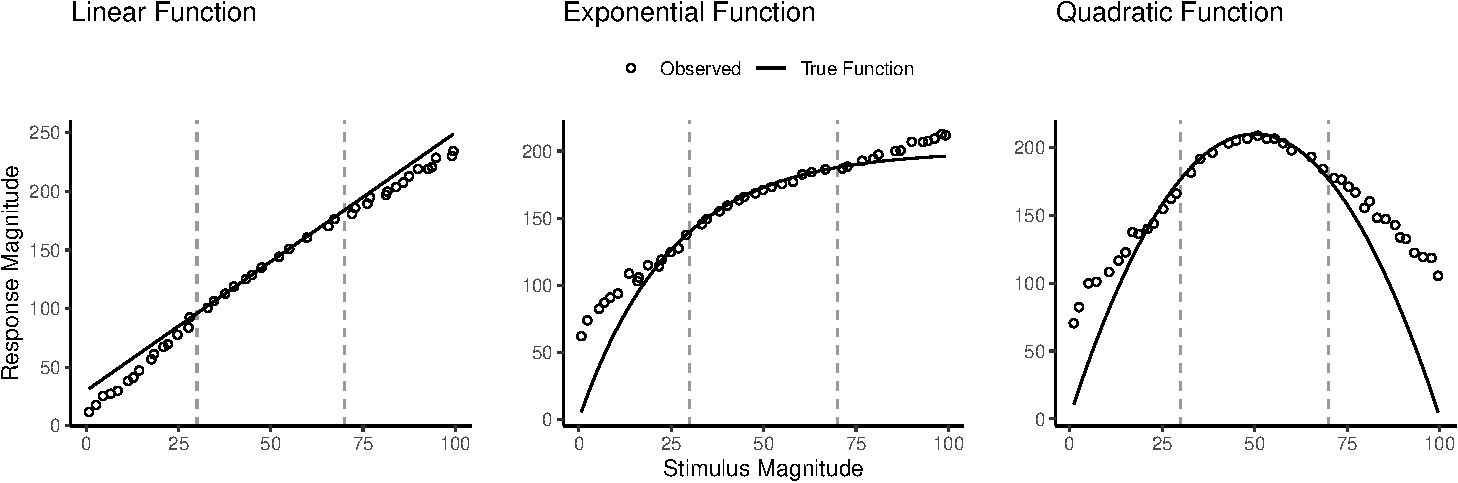
\includegraphics[keepaspectratio]{manuscript_files/figure-pdf/fig-delosh-extrap-1.pdf}}

}

\caption{\label{fig-delosh-extrap}The generalization patterns of human
participants observed in DeLosh et al.~(1997) (reproduced from Figure 3
in their manuscript). Dots represent the average responses of human
participants, and solid lines represent the true functions. The dashed
vertical lines indicate the lower and upper bounds of the trained
examples. Stimulii that fall within the dashed lines are interpolations
of the training examples, while those that fall outside the dashed lines
are extrapolations.}

\end{figure}%

\subsubsection{Variability and Function
Learning}\label{variability-and-function-learning}

The influence of variability on function learning tasks has received
relatively little attention. The study by DeLosh et al.
(\citeproc{ref-deloshExtrapolationSineQua1997}{1997}) (described in
detail above) did include a variability manipulation (referred to as
density in their paper), wherein participants were trained with either
8, 20, or 50 unique input-output pairs, with the total number of
training trials held constant. They found a minimal influence of
variability on training performance, and no difference between groups in
interpolation or extrapolation, with all three variability conditions
displaying accurate interpolation, and linearly biased extrapolation
that was well accounted for by the EXAM model.

In the domain of visuomotor learning, van Dam \& Ernst
(\citeproc{ref-vandamMappingShapeVisuomotor2015}{2015}) employed a task
which required participants to learn a linear function between the
spikiness of shape stimuli and the correct horizontal position to make a
rapid pointing response. The shapes ranged from very spiky to completely
circular at the extreme ends of the space. Participants trained with
intermediate shapes having lower variation (2 shapes) or higher
variation (5 shapes) condition, with the 2 items of the lower variation
condition matching the items used on the extreme ends of the higher
variation training space. Learning was significantly slower in the
higher variation group. However, the two conditions did not differ when
tested with novel shapes, with both groups producing extrapolation
responses of comparable magnitude to the most similar training item,
rather than in accordance with the true linear function. The authors
accounted for both learning and extrapolation performance with a
Bayesian learning model. Similar to ALM, the model assumes that
generalization occurs as a Gaussian function of the distance between
stimuli. However, unlike ALM, the Bayesian learning model utilizes more
elaborate probabilistic stimulus representations, with a separate Kalman
Filter for each shape stimulus.

\subsubsection{Overview Of Present
Study}\label{overview-of-present-study}

The present study investigates the influence of training variability on
learning, generalization, and extrapolation in a uni-dimensional
visuomotor function learning task. To the best of our knowledge, this
research is the first to employ the classic constant vs.~varied training
manipulation, commonly used in the literature studying the benefits of
variability, in the context of a uni-dimensional function learning task.
Across three experiments, we compare constant and varied training
conditions in terms of learning performance, extrapolation accuracy, and
the ability to reliably discriminate between stimuli.

To account for the empirical results, we will apply a series of
computational models, including the Associative Learning Model (ALM) and
the Extrapolation-Association Model (EXAM). Notably, this study is the
first to employ approximate Bayesian computation (ABC) to fit these
models to individual subject data, enabling us to thoroughly investigate
the full range of posterior predictions of each model, and to examine
the ability of these influential models of function learning to account
for both the group level and individual level data.

\subsection{Experiment 1}\label{experiment-1-1}

\subsubsection{Methods}\label{methods-2}

\emph{Participants.} A total of 183 participants were initially
recruited from Indiana University Introductory Psychology Courses. Of
these, 27 participants were excluded from further analysis due to
meeting the exclusion criteria, resulting in a final sample of 156
participants. The exclusion criteria was defined as performance worse
(i.e., larger deviations) than the condition average in either the
training or testing stage of the experiment. The remaining participants
were randomly assigned to one of two training conditions: varied
training or constant training.

\emph{Task.} The ``Hit The Wall'' (HTW) visuomotor extrapolation task
was programmed in JavaScript, making use of the
\href{https://phaser.io/}{phaser.io} game library. The HTW task involved
launching a projectile such that it would strike the ``wall'' at the
target speed indicated at the top of the screen (see
Figure~\ref{fig-htw-task}). The target velocities were given as a range,
or band, of acceptable velocity values (e.g., band 800-1000). During the
training stage, participants received feedback indicating whether they
had hit the wall within the target velocity band, or how many units
their throw was above or below the target band. Participants were
instructed that only the x velocity component of the ball was relevant
to the task. The y velocity, or the location at which the ball struck
the wall, had no influence on the task feedback.

\begin{figure}

\centering{

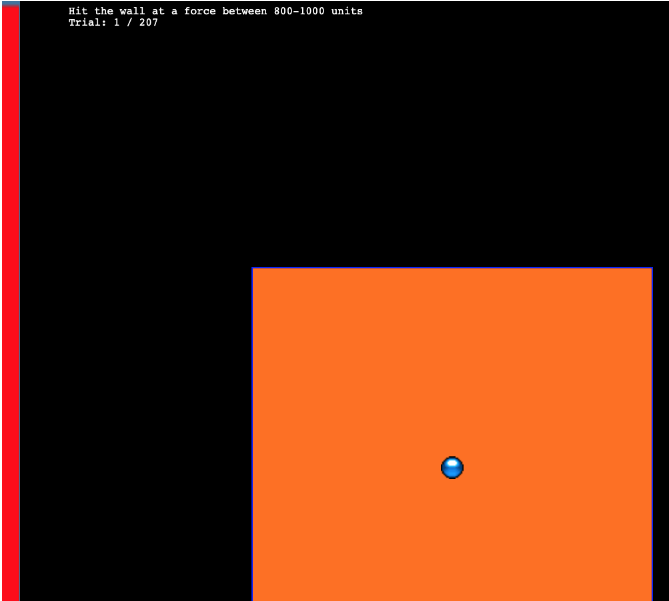
\includegraphics[width=0.6\linewidth,height=\textheight,keepaspectratio]{../Assets/figs/htw_task_fig.png}

}

\caption{\label{fig-htw-task}The Hit the wall task. Participants launch
the blue ball to hit the red wall at the target velocity band indicated
at the top of the screen. The ball must be released from within the
orange square - but the location of release, and the location at which
the ball strikes the wall are both irrelevant to the task feedback.}

\end{figure}%

\emph{Procedure.} All participants completed the task online.
Participants were provided with a description of the experiment and
indicated informed consent. Figure~\ref{fig-design-e1} illustrates the
general procedure. Participants completed a total of 90 trials during
the training stage. In the varied training condition, participants
encountered three velocity bands (800-1000, 1000-1200, and 1200-1400).
Participants in the constant training condition trained on only one
velocity band (800-1000) - the closest band to what would be the novel
extrapolation bands in the testing stage.

Following the training stage, participants proceeded immediately to the
testing stage. Participants were tested from all six velocity bands, in
two separate stages. In the novel extrapolation testing stage,
participants completed ``no-feedback'' testing from three novel
extrapolation bands (100-300, 350-550, and 600-800), with each band
consisting of 15 trials. Participants were also tested from the three
velocity bands that were trained by the varied condition (800-1000,
1000-1200, and 1200-1400). In the constant training condition, two of
these bands were novel, while in the varied training condition, all
three bands were encountered during training. The order in which
participants completed the novel-extrapolation and testing-from-3-varied
bands was counterbalanced across participants. A final training stage
presented participants with ``feedback'' testing for each of the three
extrapolation bands (100-300, 350-550, and 600-800).

\begin{figure}

\centering{

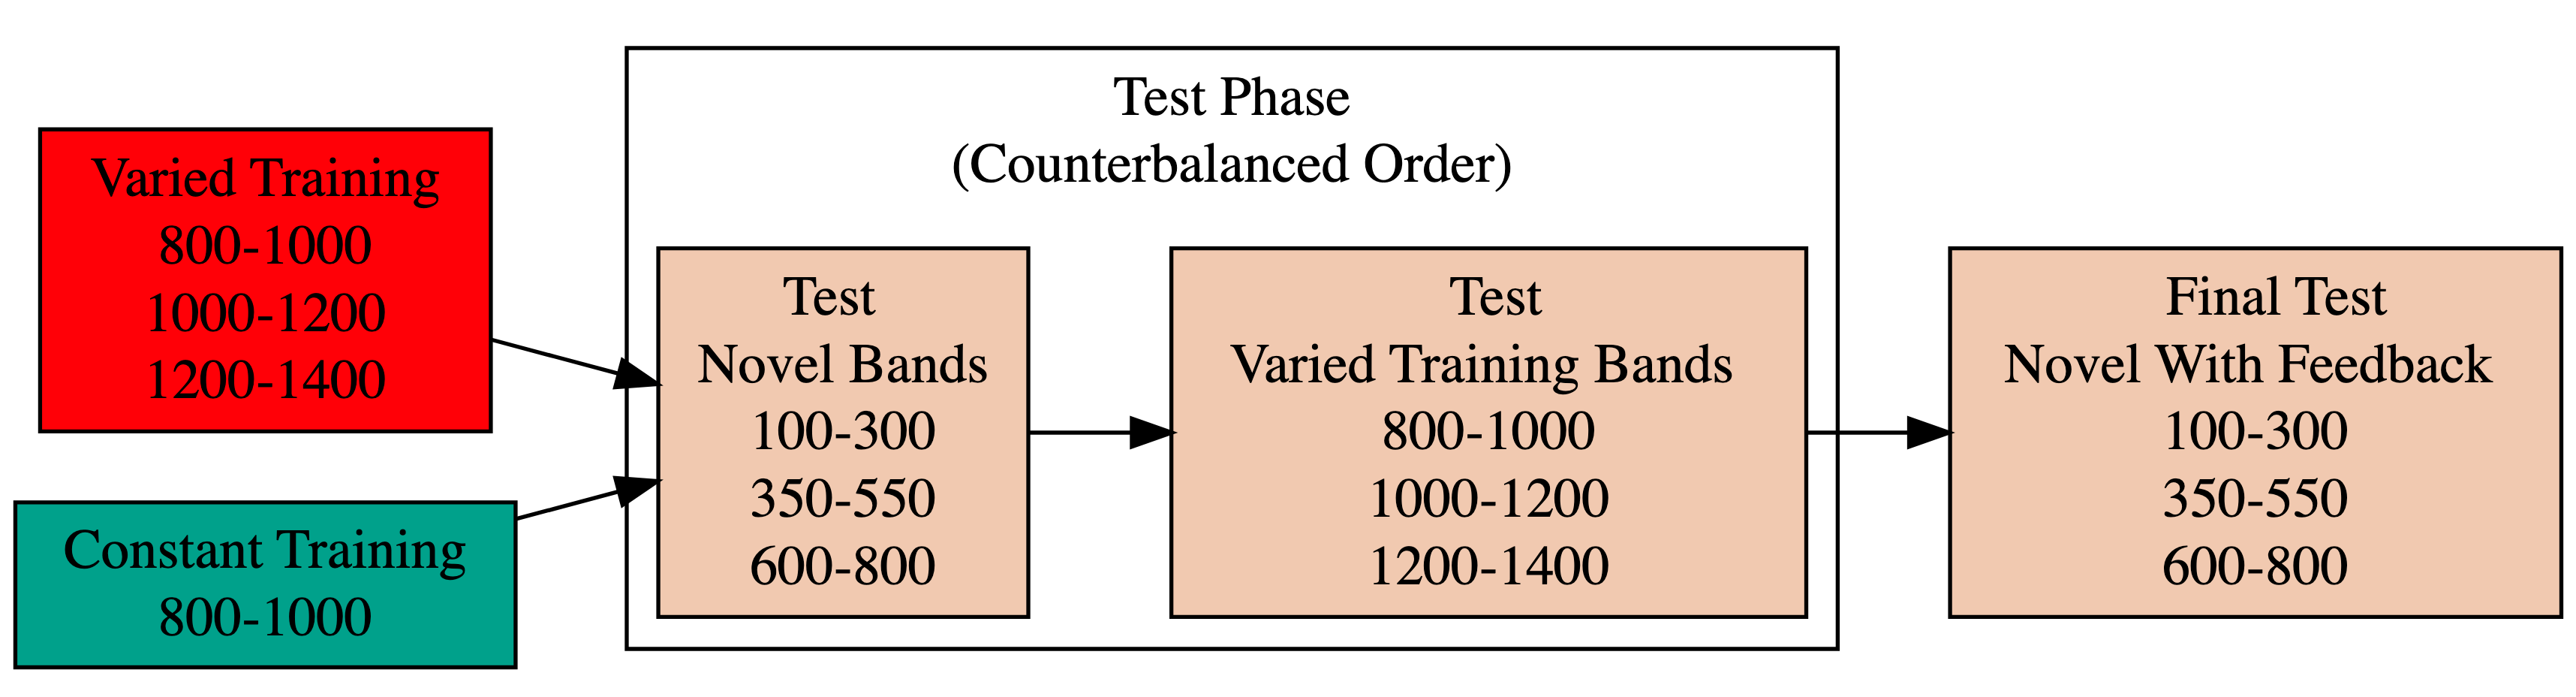
\includegraphics[width=7in,height=2.5in]{manuscript_files/figure-latex/dot-figure-1.png}

}

\caption{\label{fig-design-e1}Experiment 1 Design. Constant and Varied
participants complete different training conditions.}

\end{figure}%

\subsubsection{Analyses Strategy}\label{analyses-strategy}

All data processing and statistical analyses were performed in R version
4.32 (\citeproc{ref-rcoreteamLanguageEnvironmentStatistical2020}{Team,
2020}). To assess differences between groups, we used Bayesian Mixed
Effects Regression. Model fitting was performed with the brms package in
R (\citeproc{ref-burknerBrmsPackageBayesian2017}{Bürkner, 2017}), and
descriptive stats and tables were extracted with the BayestestR package
(\citeproc{ref-makowskiBayestestRDescribingEffects2019}{Makowski et al.,
2019}). Mixed effects regression enables us to take advantage of partial
pooling, simultaneously estimating parameters at the individual and
group level. Our use of Bayesian, rather than frequentist methods allows
us to directly quantify the uncertainty in our parameter estimates, as
well as avoid convergence issues common to the frequentist analogues of
our mixed models.

Each model was set to run with 4 chains, 5000 iterations per chain, with
the first 2500 discarded as warmup chains. Rhat values were within an
acceptable range, with values \textless=1.02 (see appendix for
diagnostic plots). We used uninformative priors for the fixed effects of
the model (condition and velocity band), and weakly informative Student
T distributions for the random effects. For each model, we report 1) the
mean values of the posterior distribution for the parameters of
interest, 2) the lower and upper credible intervals (CrI), and the
probability of direction value (pd).

\begin{longtable}[]{@{}
  >{\raggedright\arraybackslash}p{(\linewidth - 4\tabcolsep) * \real{0.2329}}
  >{\raggedright\arraybackslash}p{(\linewidth - 4\tabcolsep) * \real{0.5342}}
  >{\raggedright\arraybackslash}p{(\linewidth - 4\tabcolsep) * \real{0.2329}}@{}}
\caption{\textbf{Statistical Model Specifications}. The specifications
for the Bayesian regression models used in the analyses of each of the 3
experiments. Comparisons of accuracy use absolute deviation as the
dependent variable, while comparisons of discrimination use the raw
velocities produced by participants as the dependent
variable.}\label{tbl-brms-models}\tabularnewline
\toprule\noalign{}
\begin{minipage}[b]{\linewidth}\raggedright
Group Comparison
\end{minipage} & \begin{minipage}[b]{\linewidth}\raggedright
Code
\end{minipage} & \begin{minipage}[b]{\linewidth}\raggedright
Data
\end{minipage} \\
\midrule\noalign{}
\endfirsthead
\toprule\noalign{}
\begin{minipage}[b]{\linewidth}\raggedright
Group Comparison
\end{minipage} & \begin{minipage}[b]{\linewidth}\raggedright
Code
\end{minipage} & \begin{minipage}[b]{\linewidth}\raggedright
Data
\end{minipage} \\
\midrule\noalign{}
\endhead
\bottomrule\noalign{}
\endlastfoot
End of Training Accuracy &
\texttt{brm(Abs.\ Deviation\ \textasciitilde{}\ condit)} & Final
Training Block \\
Test Accuracy &
\texttt{brm(Abs.\ Deviation\ \textasciitilde{}\ condit\ *\ bandType\ +\ (1\textbar{}id)\ +\ (1\textbar{}bandInt)}
& All Testing trials \\
Band Discrimination &
\texttt{brm(vx\ \textasciitilde{}\ condit\ *\ band\ +(1\ +\ bandInt\textbar{}id)}
& All Testing Trials \\
\end{longtable}

\hfill\break

In each experiment we compare varied and constant conditions in terms of
1) accuracy in the final training block; 2) testing accuracy as a
function of band type (trained vs.~extrapolation bands); 3) extent of
discrimination between all six testing bands. We quantified accuracy as
the absolute deviation between the response velocity and the nearest
boundary of the target band. Thus, when the target band was velocity
600-800, throws of 400, 650, and 900 would result in deviation values of
200, 0, and 100, respectively. The degree of discrimination between
bands was measured by fitting a linear model predicting the response
velocity as a function of the target velocity. Participants who reliably
discriminated between velocity bands tended to have slope values
\textasciitilde1, while participants who made throws irrespective of the
current target band would have slopes \textasciitilde0.

\subsubsection{Results}\label{results-2}

\begin{figure}

\centering{

\pandocbounded{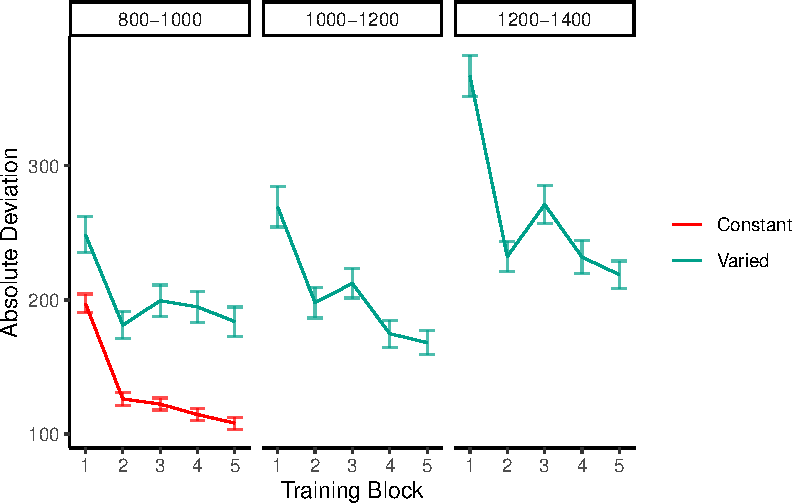
\includegraphics[keepaspectratio]{manuscript_files/figure-pdf/fig-e1-train-dev-1.pdf}}

}

\caption{\label{fig-e1-train-dev}Experiment 1 - Training Stage.
Deviations from target band across training blocks. Lower values
represent greater accuracy.}

\end{figure}%

\begin{longtable}[]{@{}lrrrr@{}}
\caption{\textbf{Experiment 1 - End of training performance}. Comparing
final training block accuracy in the band common to both groups. The
Intercept represents the average of the baseline condition (constant
training), and the conditVaried coefficient reflects the difference
between the constant and varied groups. A larger positive estimate
indicates a greater deviation (lower accuracy) for the varied group. CrI
values indicate 95\% credible intervals. pd is the probability of
direction (the \% of the posterior on the same side of 0 as the
coefficient estimate).}\label{tbl-e1-train-dist}\tabularnewline
\toprule\noalign{}
Term & Estimate & 95\% CrI Lower & 95\% CrI Upper & pd \\
\midrule\noalign{}
\endfirsthead
\toprule\noalign{}
Term & Estimate & 95\% CrI Lower & 95\% CrI Upper & pd \\
\midrule\noalign{}
\endhead
\bottomrule\noalign{}
\endlastfoot
Intercept & 106.34 & 95.46 & 117.25 & 1 \\
conditVaried & 79.64 & 57.92 & 101.63 & 1 \\
\end{longtable}

\hfill\break

\emph{Training}. Figure~\ref{fig-e1-train-dev} displays the average
deviations across training blocks for the varied group, which trained on
three velocity bands, and the constant group, which trained on one
velocity band. To compare the training conditions at the end of
training, we analyzed performance on the 800-1000 velocity band, which
both groups trained on. The full model results are shown in Table 1. The
varied group had a significantly greater deviation from the target band
than the constant group in the final training block, (\(\beta\) = 79.64,
95\% CrI {[}57.92, 101.63{]}; pd = 100\%).

\begin{longtable}[]{@{}
  >{\raggedright\arraybackslash}p{(\linewidth - 8\tabcolsep) * \real{0.3425}}
  >{\raggedleft\arraybackslash}p{(\linewidth - 8\tabcolsep) * \real{0.1644}}
  >{\raggedleft\arraybackslash}p{(\linewidth - 8\tabcolsep) * \real{0.1644}}
  >{\raggedleft\arraybackslash}p{(\linewidth - 8\tabcolsep) * \real{0.1644}}
  >{\raggedleft\arraybackslash}p{(\linewidth - 8\tabcolsep) * \real{0.1644}}@{}}
\caption{\textbf{Experiment 1 testing accuracy}. Main effects of
condition and band type (training vs.~extrapolation bands), and the
interaction between the two factors. The Intercept represents the
baseline condition (constant training \& trained bands). Larger
coefficients indicate larger deviations from the baselines - and a
positive interaction coefficient indicates disproportionate deviation
for the varied condition on the extrapolation bands. CrI values indicate
95\% credible intervals. pd is the probability of direction (the \% of
the posterior on the same side of 0 as the coefficient
estimate).}\label{tbl-e1-bmm-dist}\tabularnewline
\toprule\noalign{}
\begin{minipage}[b]{\linewidth}\raggedright
Term
\end{minipage} & \begin{minipage}[b]{\linewidth}\raggedleft
Estimate
\end{minipage} & \begin{minipage}[b]{\linewidth}\raggedleft
95\% CrI Lower
\end{minipage} & \begin{minipage}[b]{\linewidth}\raggedleft
95\% CrI Upper
\end{minipage} & \begin{minipage}[b]{\linewidth}\raggedleft
pd
\end{minipage} \\
\midrule\noalign{}
\endfirsthead
\toprule\noalign{}
\begin{minipage}[b]{\linewidth}\raggedright
Term
\end{minipage} & \begin{minipage}[b]{\linewidth}\raggedleft
Estimate
\end{minipage} & \begin{minipage}[b]{\linewidth}\raggedleft
95\% CrI Lower
\end{minipage} & \begin{minipage}[b]{\linewidth}\raggedleft
95\% CrI Upper
\end{minipage} & \begin{minipage}[b]{\linewidth}\raggedleft
pd
\end{minipage} \\
\midrule\noalign{}
\endhead
\bottomrule\noalign{}
\endlastfoot
Intercept & 152.55 & 70.63 & 229.85 & 1.0 \\
conditVaried & 39.00 & -21.10 & 100.81 & 0.9 \\
bandTypeExtrapolation & 71.51 & 33.24 & 109.60 & 1.0 \\
conditVaried:bandTypeExtrapolation & 66.46 & 32.76 & 99.36 & 1.0 \\
\end{longtable}

\emph{Testing.} To compare accuracy between groups in the testing stage,
we fit a Bayesian mixed effects model predicting deviation from the
target band as a function of training condition (varied vs.~constant)
and band type (trained vs.~extrapolation), with random intercepts for
participants and bands. The model results are shown in
Table~\ref{tbl-e1-bmm-dist}. The main effect of training condition was
not significant (\(\beta\) = 39, 95\% CrI {[}-21.1, 100.81{]}; pd =
89.93\%). The extrapolation testing items had a significantly greater
deviation than the training bands (\(\beta\) = 71.51, 95\% CrI {[}33.24,
109.6{]}; pd = 99.99\%). Most importantly, the interaction between
training condition and band type was significant (\(\beta\) = 66.46,
95\% CrI {[}32.76, 99.36{]}; pd = 99.99\%), As shown in
Figure~\ref{fig-e1-test-dev}, the varied group had disproportionately
larger deviations compared to the constant group in the extrapolation
bands.

\begin{figure}

\centering{

\pandocbounded{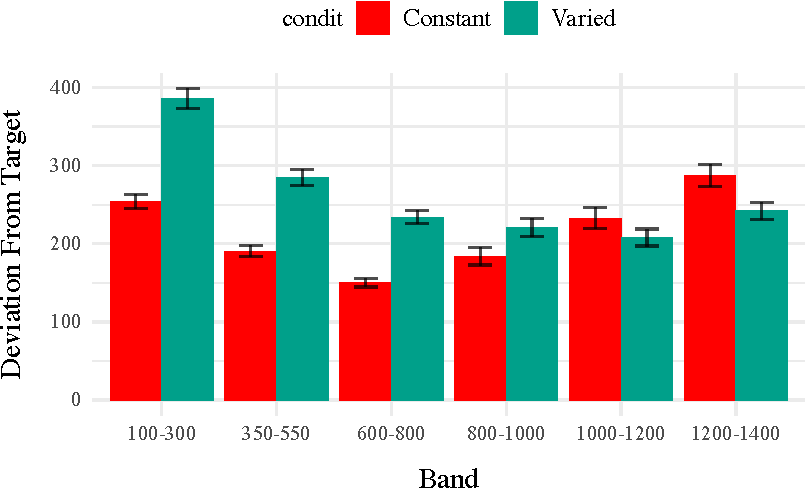
\includegraphics[keepaspectratio]{manuscript_files/figure-pdf/fig-e1-test-dev-1.pdf}}

}

\caption{\label{fig-e1-test-dev}Experiment 1 Testing Accuracy. A)
Empirical Deviations from target band during testing without feedback
stage. B) Conditional effect of condition (Constant vs.~Varied) and
testing band type (trained bands vs.~novel extrapolation bands) on
testing accuracy. Error bars represent 95\% credible intervals.}

\end{figure}%

\hfill\break

\begin{longtable}[]{@{}lrrrr@{}}
\caption{\textbf{Experiment 1 Testing Discrimination}. Bayesian Mixed
Model Predicting velocity as a function of condition (Constant
vs.~Varied) and Velocity Band. Larger coefficients for the Band term
reflect a larger slope, or greater sensitivity/discrimination. The
interaction between condit and Band indicates the difference between
constant and varied slopes. CrI values indicate 95\% credible intervals.
pd is the probability of direction (the \% of the posterior on the same
side of 0 as the coefficient
estimate).}\label{tbl-e1-bmm-vx}\tabularnewline
\toprule\noalign{}
Term & Estimate & 95\% CrI Lower & 95\% CrI Upper & pd \\
\midrule\noalign{}
\endfirsthead
\toprule\noalign{}
Term & Estimate & 95\% CrI Lower & 95\% CrI Upper & pd \\
\midrule\noalign{}
\endhead
\bottomrule\noalign{}
\endlastfoot
Intercept & 408.55 & 327.00 & 490.61 & 1.00 \\
conditVaried & 164.05 & 45.50 & 278.85 & 1.00 \\
Band & 0.71 & 0.62 & 0.80 & 1.00 \\
condit*Band & -0.14 & -0.26 & -0.01 & 0.98 \\
\end{longtable}

Finally, to assess the ability of both conditions to discriminate
between velocity bands, we fit a model predicting velocity as a function
of training condition and velocity band, with random intercepts and
random slopes for each participant. See Table~\ref{tbl-e1-bmm-vx} for
the full model results. The estimated coefficient for training condition
(\(\beta\) = 164.05, 95\% CrI {[}45.5, 278.85{]}, pd = 99.61\%) suggests
that the varied group tends to produce harder throws than the constant
group, though this is not, in and of itself, useful for assessing
discrimination. Most relevant to the issue of discrimination is the
coefficient on the Band predictor (\(\beta\) = 0.71 95\% CrI {[}0.62,
0.8{]}, pd = 100\%). Although the median slope does fall underneath the
ideal of value of 1, the fact that the 95\% credible interval does not
contain 0 provides strong evidence that participants exhibited some
discrimination between bands. The significant negative estimate for the
interaction between slope and condition (\(\beta\) = -0.14, 95\% CrI
{[}-0.26, -0.01{]}, pd = 98.39\%), indicates that the discrimination was
modulated by training condition, with the varied participants showing
less sensitivity between bands than the constant condition (see
Figure~\ref{fig-e1-test-vx} and Figure~\ref{fig-e1-bmm-vx}).

\begin{figure}

\centering{

\pandocbounded{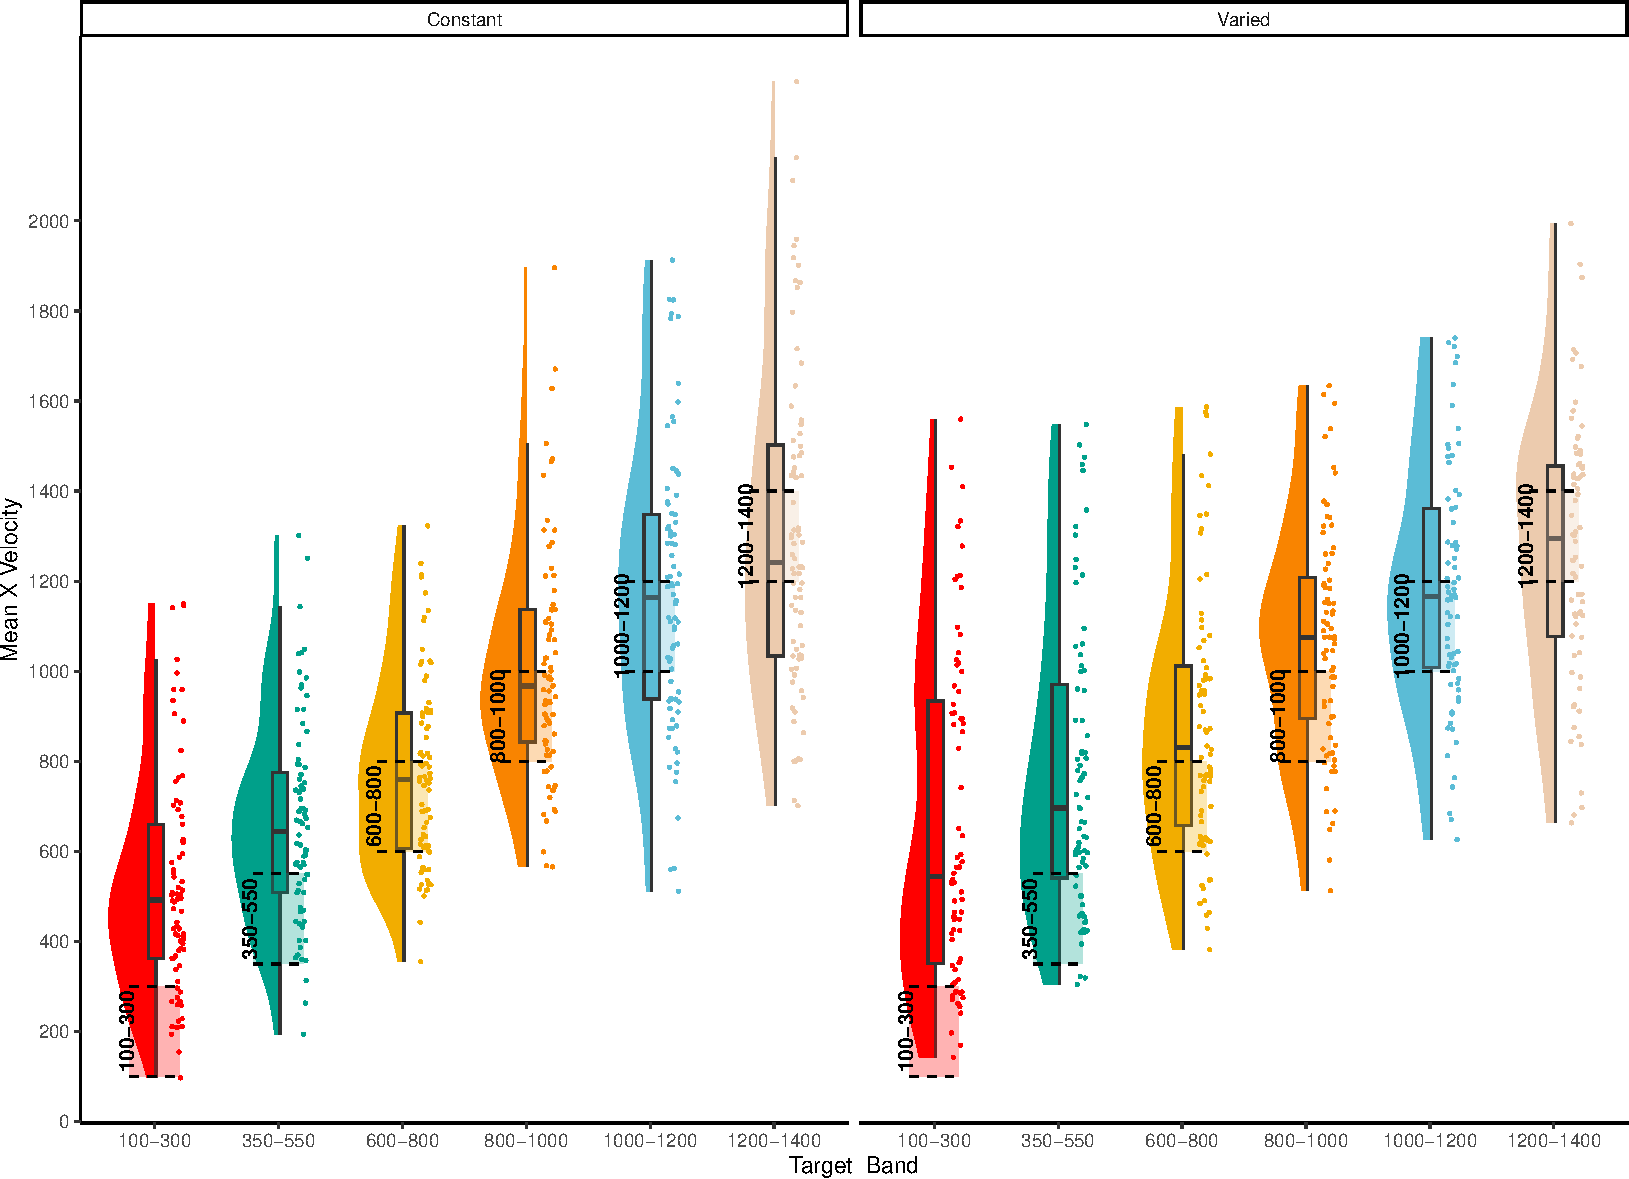
\includegraphics[keepaspectratio]{manuscript_files/figure-pdf/fig-e1-test-vx-1.pdf}}

}

\caption{\label{fig-e1-test-vx}Experiment 1. Empirical distribution of
velocities produced in the testing stage. Translucent bands with dashed
lines indicate the correct range for each velocity band.}

\end{figure}%

\begin{figure}

\centering{

\pandocbounded{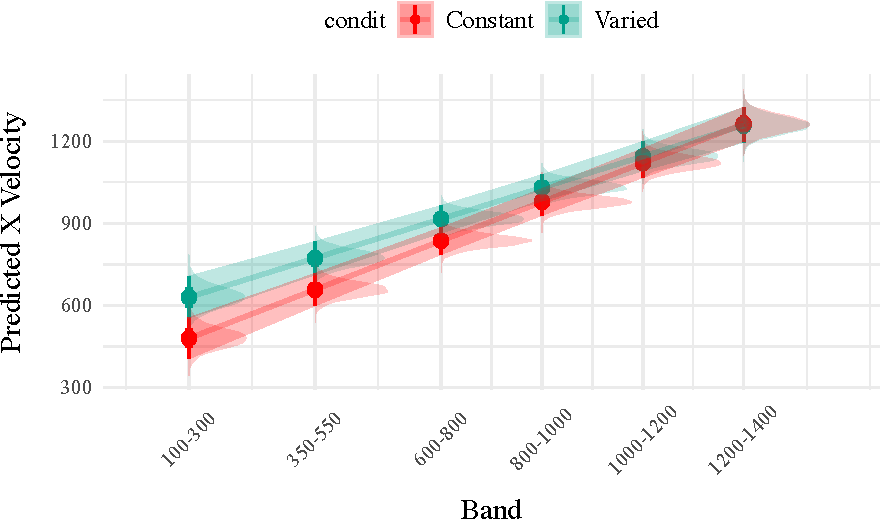
\includegraphics[keepaspectratio]{manuscript_files/figure-pdf/fig-e1-bmm-vx-1.pdf}}

}

\caption{\label{fig-e1-bmm-vx}Experiment 1 Discrimination. A)
Conditional effect of training condition and Band. Ribbons indicate 95\%
HDI. The steepness of the lines serves as an indicator of how well
participants discriminated between velocity bands. B) The distribution
of slope coefficients for each condition. Larger slopes indicate better
discrimination between target bands. C) Individual participant slopes.
Error bars represent 95\% HDI.}

\end{figure}%

\subsubsection{Experiment 1 Summary}\label{experiment-1-summary}

In Experiment 1, we investigated how variability in training influenced
participants' ability to learn and extrapolate in a visuomotor task. Our
findings that training with variable conditions resulted in lower final
training performance are consistent with much of the prior research on
the influence of training variability
(\citeproc{ref-ravivHowVariabilityShapes2022}{Raviv et al., 2022};
\citeproc{ref-soderstromLearningPerformanceIntegrative2015}{Soderstrom
\& Bjork, 2015}), and are particularly unsurprising in the present work,
given that the constant group received three times the amount of
training on the velocity band common to the two conditions.

More importantly, the varied training group exhibited significantly
larger deviations from the target velocity bands during the testing
phase, particularly for the extrapolation bands that were not
encountered by either condition during training.

\subsection{Experiment 2}\label{experiment-2-1}

\subsubsection{Methods \& Procedure}\label{methods-procedure}

Initially, 131 participants were recruited. After applying the same
exclusion procedure as in Experiment 1, 21 participants were excluded,
resulting in a final sample of 110 participants who completed the
experiment (Varied: 55, Constant: 55). The task and procedure of
Experiment 2 was identical to Experiment 1, with the exception that the
training and testing bands were reversed (see
Figure~\ref{fig-design-e2}). The Varied group trained on bands 100-300,
350-550, 600-800, and the constant group trained on band 600-800. Both
groups were tested from all six bands.

\begin{figure}

\centering{

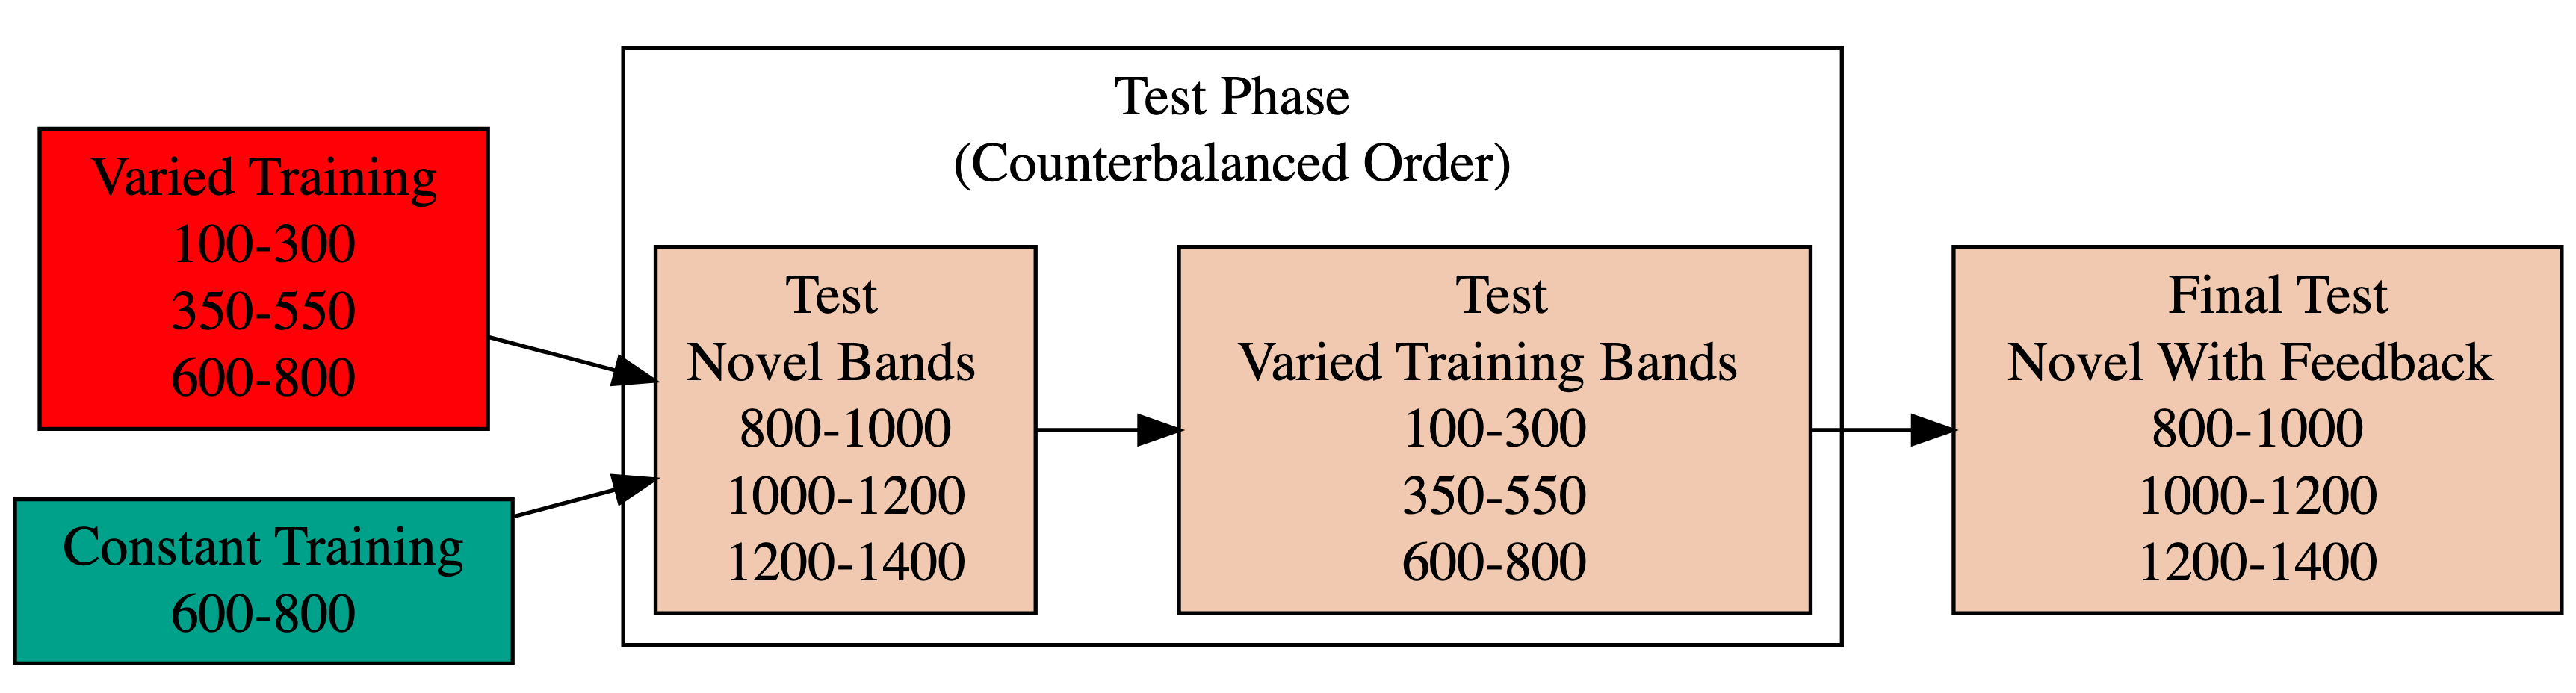
\includegraphics[width=7in,height=2.2in]{manuscript_files/figure-latex/dot-figure-2.png}

}

\caption{\label{fig-design-e2}Experiment 2 Design. Constant and Varied
participants complete different training conditions. The training and
testing bands are the reverse of Experiment 1.}

\end{figure}%

\subsubsection{Results}\label{results-3}

\begin{figure}

\centering{

\pandocbounded{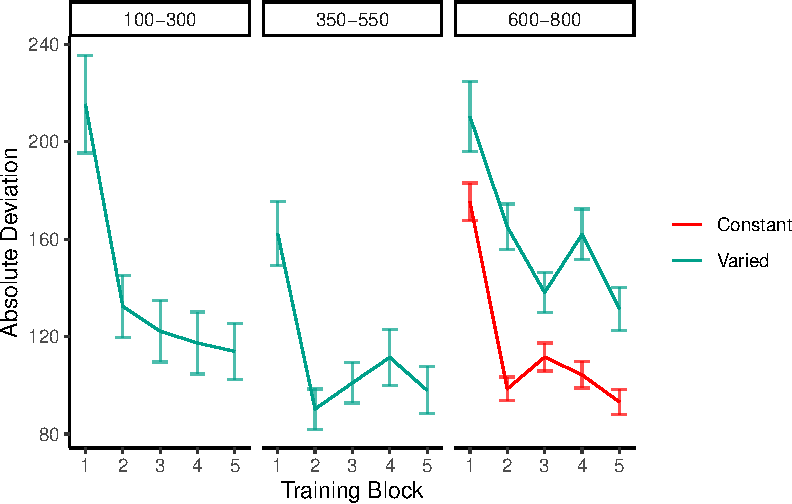
\includegraphics[keepaspectratio]{manuscript_files/figure-pdf/fig-e2-train-dev-1.pdf}}

}

\caption{\label{fig-e2-train-dev}Experiment 2 Training Stage. Deviations
from target band across training blocks. Lower values represent greater
accuracy.}

\end{figure}%

\begin{longtable}[]{@{}lrrrr@{}}
\caption{\textbf{Experiment 2 - End of training performance}. The
Intercept represents the average of the baseline condition (constant
training), and the conditVaried coefficient reflects the difference
between the constant and varied groups. A larger positive coefficient
indicates a greater deviation (lower accuracy) for the varied group. CrI
values indicate 95\% credible intervals. pd is the probability of
direction (the \% of the posterior on the same side of 0 as the
coefficient estimate).}\label{tbl-e2-train-dist}\tabularnewline
\toprule\noalign{}
Term & Estimate & 95\% CrI Lower & 95\% CrI Upper & pd \\
\midrule\noalign{}
\endfirsthead
\toprule\noalign{}
Term & Estimate & 95\% CrI Lower & 95\% CrI Upper & pd \\
\midrule\noalign{}
\endhead
\bottomrule\noalign{}
\endlastfoot
Intercept & 91.01 & 80.67 & 101.26 & 1 \\
conditVaried & 36.15 & 16.35 & 55.67 & 1 \\
\end{longtable}

\hfill\break

\emph{Training}. Figure~\ref{fig-e2-train-dev} presents the deviations
across training blocks for both constant and varied training groups. We
again compared training performance on the band common to both groups
(600-800). The full model results are shown in Table 1. The varied group
had a significantly greater deviation than the constant group in the
final training block, ( \(\beta\) = 36.15, 95\% CrI {[}16.35, 55.67{]};
pd = 99.95\%).

\begin{longtable}[]{@{}
  >{\raggedright\arraybackslash}p{(\linewidth - 8\tabcolsep) * \real{0.4390}}
  >{\raggedleft\arraybackslash}p{(\linewidth - 8\tabcolsep) * \real{0.1220}}
  >{\raggedleft\arraybackslash}p{(\linewidth - 8\tabcolsep) * \real{0.1829}}
  >{\raggedleft\arraybackslash}p{(\linewidth - 8\tabcolsep) * \real{0.1829}}
  >{\raggedleft\arraybackslash}p{(\linewidth - 8\tabcolsep) * \real{0.0732}}@{}}
\caption{\textbf{Experiment 2 testing accuracy}. Main effects of
condition and band type (training vs.~extrapolation), and the
interaction between the two factors. The Intercept represents the
baseline condition (constant training \& trained bands). Larger
coefficients indicate larger deviations from the baselines - and a
positive interaction coefficient indicates disproportionate deviation
for the varied condition on the extrapolation bands. CrI values indicate
95\% credible intervals. pd is the probability of direction (the \% of
the posterior on the same side of 0 as the coefficient
estimate).}\label{tbl-e2-bmm-dist}\tabularnewline
\toprule\noalign{}
\begin{minipage}[b]{\linewidth}\raggedright
Term
\end{minipage} & \begin{minipage}[b]{\linewidth}\raggedleft
Estimate
\end{minipage} & \begin{minipage}[b]{\linewidth}\raggedleft
95\% CrI Lower
\end{minipage} & \begin{minipage}[b]{\linewidth}\raggedleft
95\% CrI Upper
\end{minipage} & \begin{minipage}[b]{\linewidth}\raggedleft
pd
\end{minipage} \\
\midrule\noalign{}
\endfirsthead
\toprule\noalign{}
\begin{minipage}[b]{\linewidth}\raggedright
Term
\end{minipage} & \begin{minipage}[b]{\linewidth}\raggedleft
Estimate
\end{minipage} & \begin{minipage}[b]{\linewidth}\raggedleft
95\% CrI Lower
\end{minipage} & \begin{minipage}[b]{\linewidth}\raggedleft
95\% CrI Upper
\end{minipage} & \begin{minipage}[b]{\linewidth}\raggedleft
pd
\end{minipage} \\
\midrule\noalign{}
\endhead
\bottomrule\noalign{}
\endlastfoot
Intercept & 190.91 & 125.03 & 259.31 & 1.00 \\
conditVaried & -20.58 & -72.94 & 33.08 & 0.78 \\
bandTypeExtrapolation & 38.09 & -6.94 & 83.63 & 0.95 \\
conditVaried:bandTypeExtrapolation & 82.00 & 41.89 & 121.31 & 1.00 \\
\end{longtable}

~\\

\emph{Testing Accuracy.} The analysis of testing accuracy examined
deviations from the target band as influenced by training condition
(Varied vs.~Constant) and band type (training vs.~extrapolation bands).
The results, summarized in Table~\ref{tbl-e2-bmm-dist}, reveal no
significant main effect of training condition (\(\beta\) = -20.58, 95\%
CrI {[}-72.94, 33.08{]}; pd = 77.81\%). However, the interaction between
training condition and band type was significant (\(\beta\) = 82, 95\%
CrI {[}41.89, 121.31{]}; pd = 100\%), with the varied group showing
disproportionately larger deviations compared to the constant group on
the extrapolation bands (see Figure~\ref{fig-e2-test-dev}).

\begin{figure}

\centering{

\pandocbounded{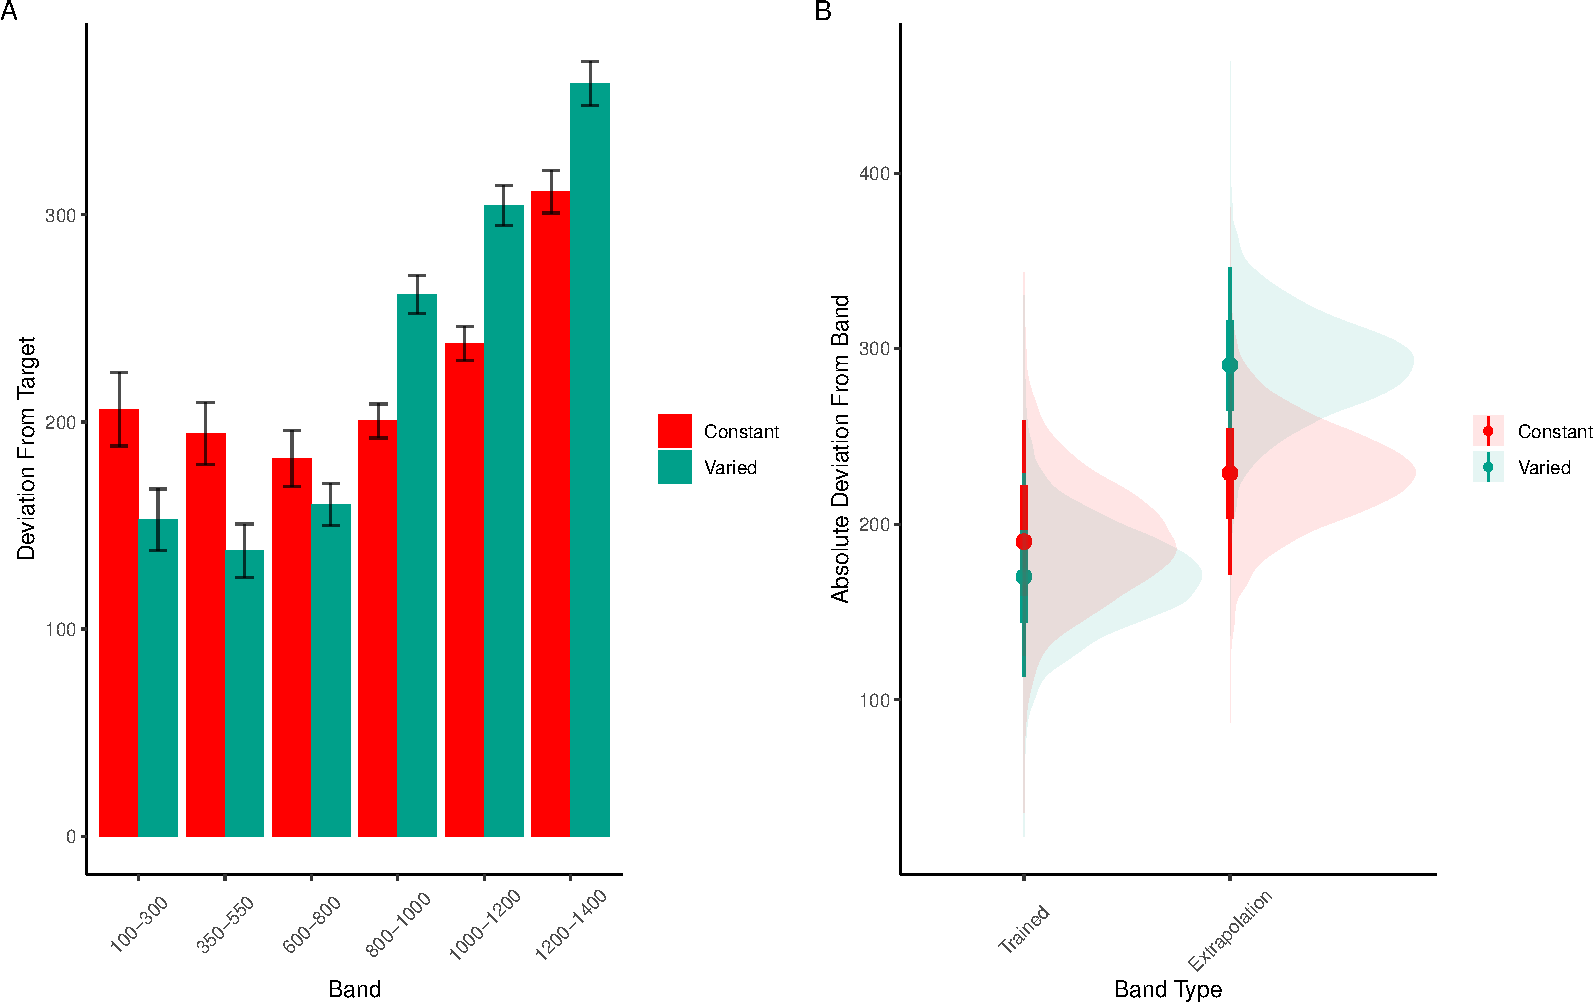
\includegraphics[keepaspectratio]{manuscript_files/figure-pdf/fig-e2-test-dev-1.pdf}}

}

\caption{\label{fig-e2-test-dev}Experiment 2 Testing Accuracy. A)
Empirical Deviations from target band during testing without feedback
stage. B) Conditional effect of condition (Constant vs.~Varied) and
testing band type (trained bands vs.~novel extrapolation bands) on
testing accuracy. Error bars represent 95\% credible intervals.}

\end{figure}%

\begin{longtable}[]{@{}lrrrr@{}}
\caption{\textbf{Experiment 2 Testing Discrimination}. Bayesian Mixed
Model Predicting velocity as a function of condition (Constant
vs.~Varied) and Velocity Band. Larger coefficients for the Band term
reflect a larger slope, or greater sensitivity/discrimination. The
interaction between condition and Band indicates the difference between
constant and varied slopes. CrI values indicate 95\% credible intervals.
pd is the probability of direction (the \% of the posterior on the same
side of 0 as the coefficient
estimate)}\label{tbl-e2-bmm-vx}\tabularnewline
\toprule\noalign{}
Term & Estimate & 95\% CrI Lower & 95\% CrI Upper & pd \\
\midrule\noalign{}
\endfirsthead
\toprule\noalign{}
Term & Estimate & 95\% CrI Lower & 95\% CrI Upper & pd \\
\midrule\noalign{}
\endhead
\bottomrule\noalign{}
\endlastfoot
Intercept & 362.64 & 274.85 & 450.02 & 1.00 \\
conditVaried & -8.56 & -133.97 & 113.98 & 0.55 \\
Band & 0.71 & 0.58 & 0.84 & 1.00 \\
condit*Band & -0.06 & -0.24 & 0.13 & 0.73 \\
\end{longtable}

\emph{Testing Discrimination.} Finally, to assess the ability of both
conditions to discriminate between velocity bands, we fit a model
predicting velocity as a function of training condition and velocity
band, with random intercepts and random slopes for each participant. The
full model results are shown in Table~\ref{tbl-e2-bmm-vx}. The overall
slope on target velocity band predictor was significantly positive,
(\(\beta\) = 0.71, 95\% CrI {[}0.58, 0.84{]}; pd= 100\%), indicating
that participants exhibited discrimination between bands. The
interaction between slope and condition was not significant, (\(\beta\)
= -0.06, 95\% CrI {[}-0.24, 0.13{]}; pd= 72.67\%), suggesting that the
two conditions did not differ in their ability to discriminate between
bands (see Figure~\ref{fig-e2-test-vx} and Figure~\ref{fig-e2-bmm-vx}).

\begin{figure}

\centering{

\pandocbounded{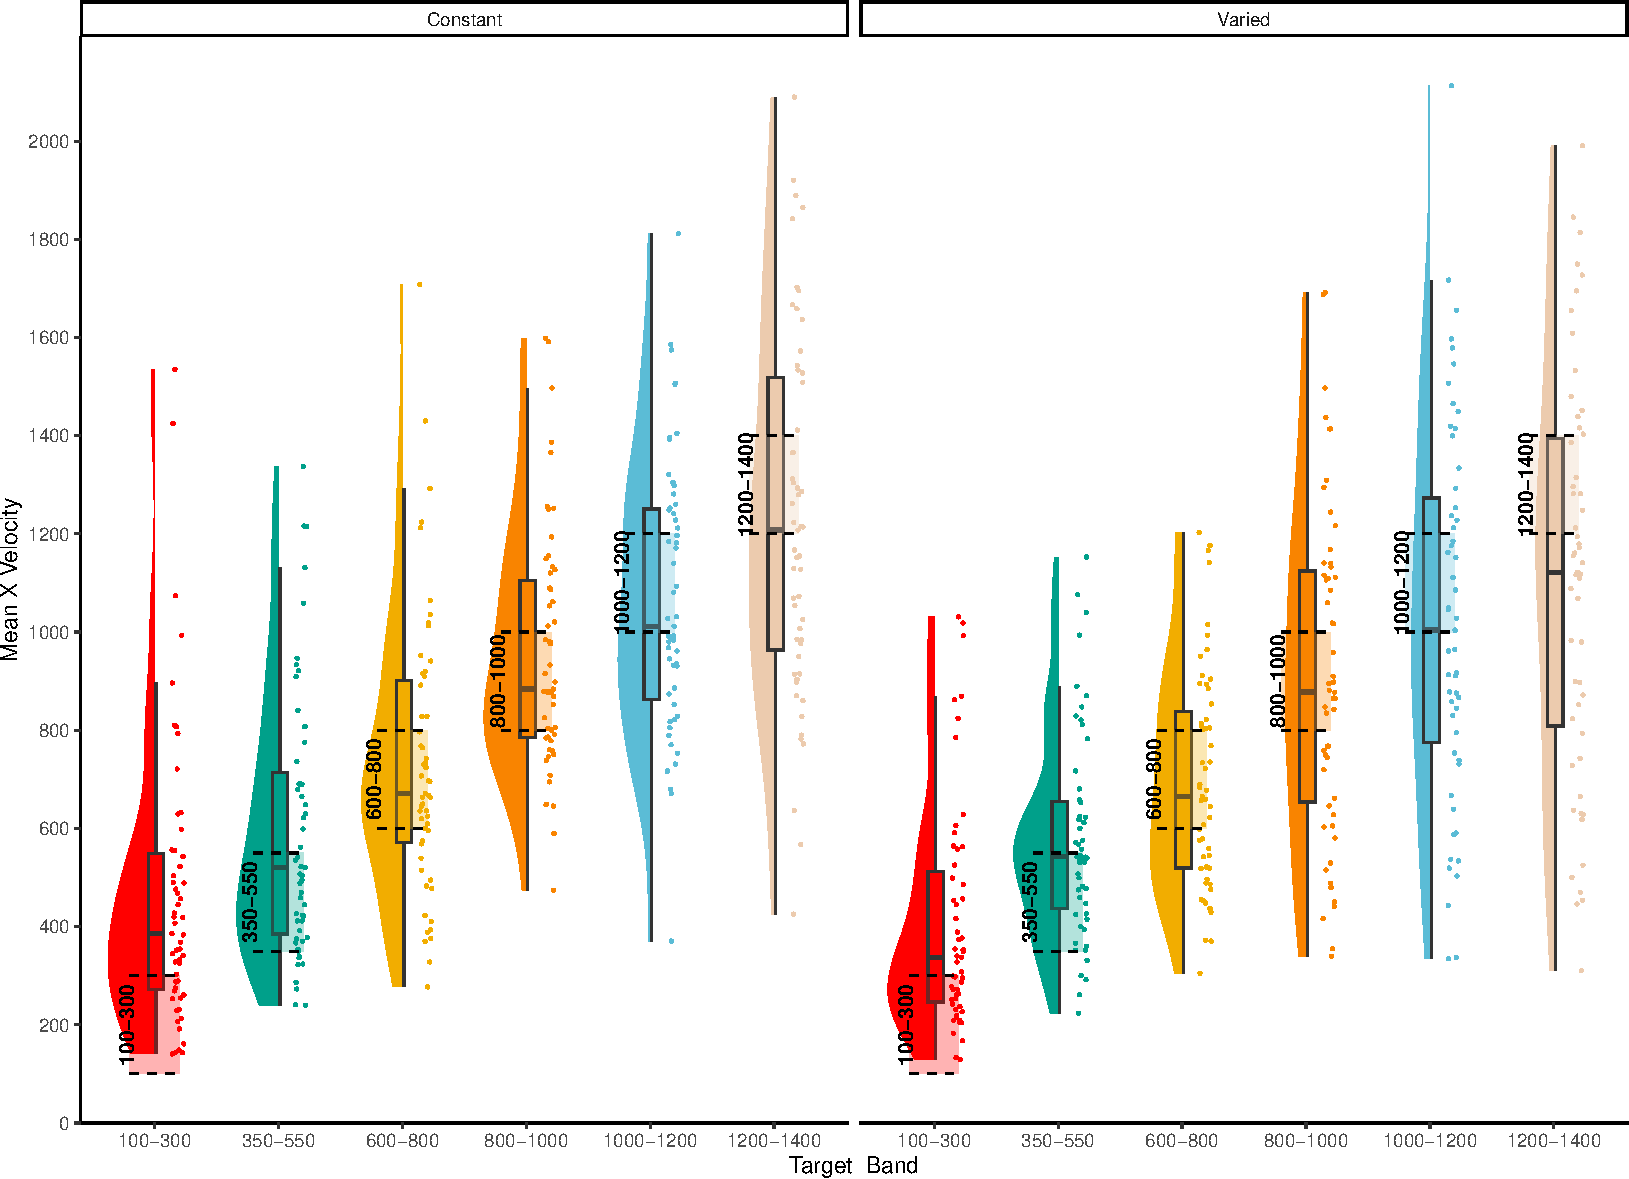
\includegraphics[keepaspectratio]{manuscript_files/figure-pdf/fig-e2-test-vx-1.pdf}}

}

\caption{\label{fig-e2-test-vx}Experiment 2. Empirical distribution of
velocities produced in the testing stage. Translucent bands with dash
lines indicate the correct range for each velocity band.}

\end{figure}%

\begin{figure}

\centering{

\pandocbounded{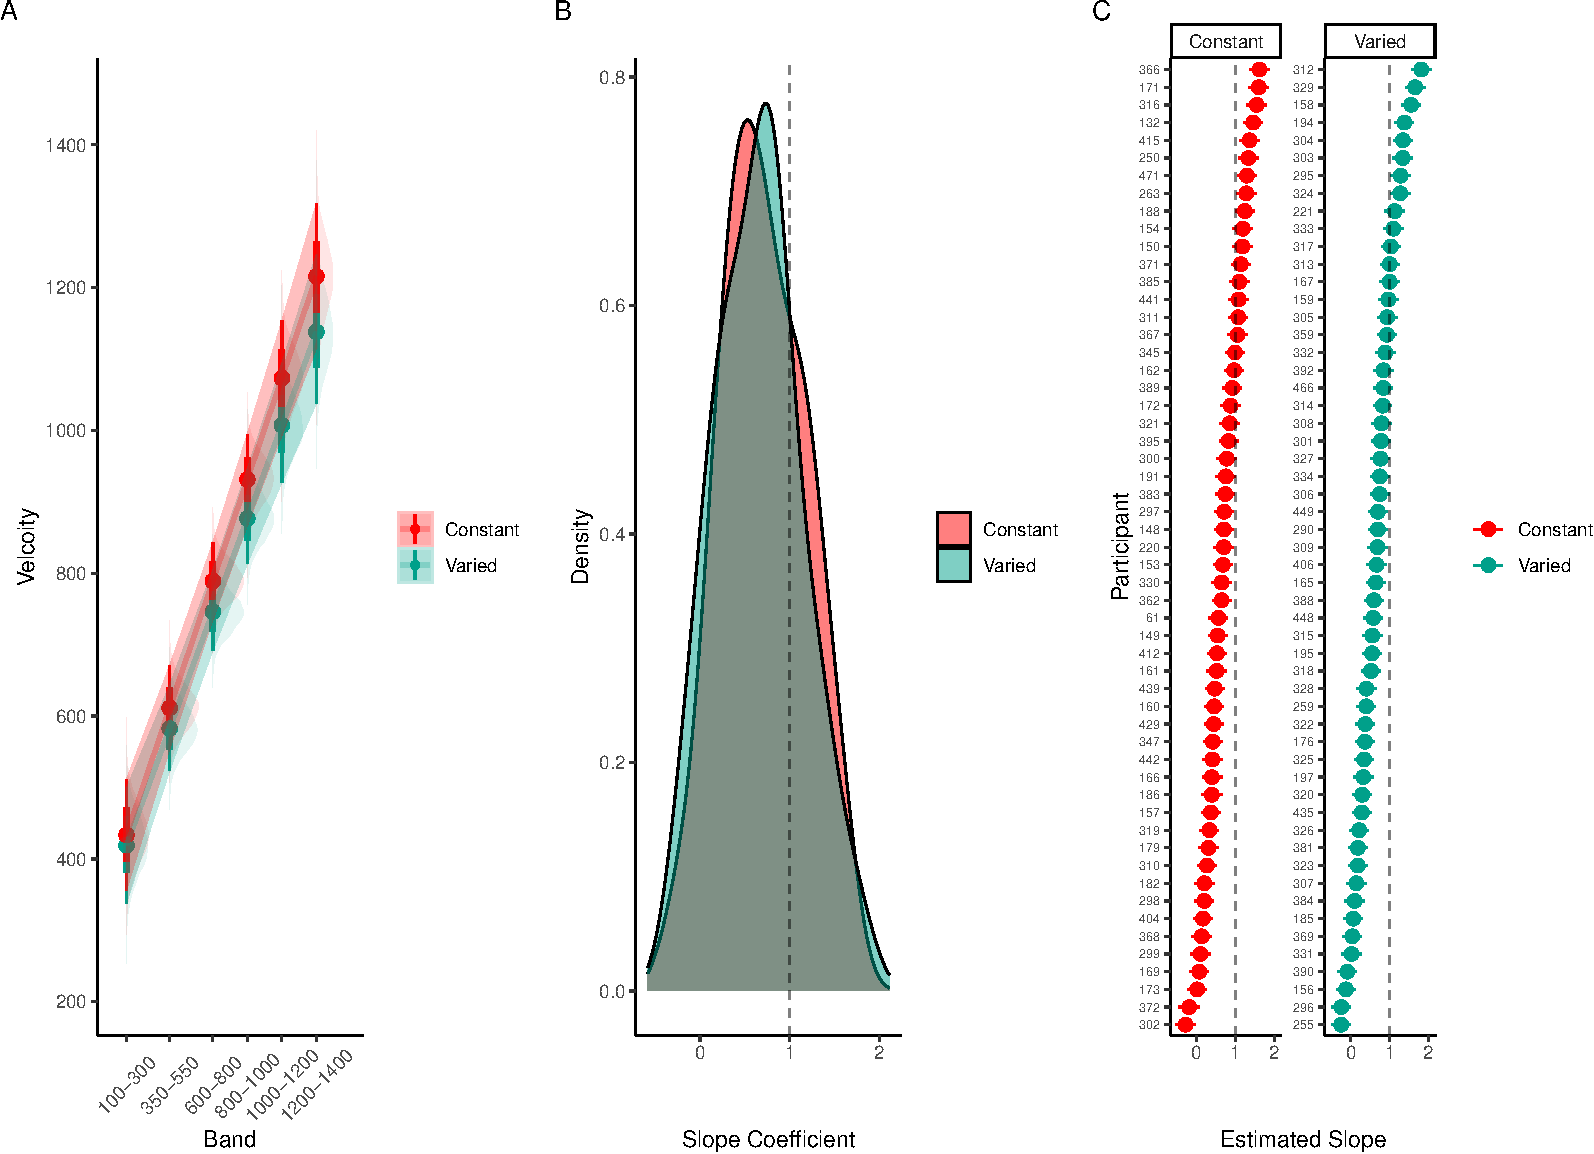
\includegraphics[keepaspectratio]{manuscript_files/figure-pdf/fig-e2-bmm-vx-1.pdf}}

}

\caption{\label{fig-e2-bmm-vx}Experiment 2 Discrimination. A)
Conditional effect of training condition and Band. Ribbons indicate 95\%
HDI. The steepness of the lines serves as an indicator of how well
participants discriminated between velocity bands. B) The distribution
of slope coefficients for each condition. Larger slopes indicate better
discrimination. C) Individual participant slopes. Error bars represent
95\% HDI.}

\end{figure}%

\subsubsection{Experiment 2 Summary}\label{experiment-2-summary}

Experiment 2 extended the findings of Experiment 1 by examining the
effects of training variability on extrapolation performance in a
visuomotor function learning task, but with reversed training and
testing bands. Similar to Experiment 1, the Varied group exhibited
poorer performance during training and testing. However, unlike
experiment 1, the Varied and Constant groups did not show a significant
difference in their discrimination between bands.

\subsection{Experiment 3}\label{experiment-3}

In Experiment 3, we sought to further explore the generality of the
findings from the first two experiments by modifying the type of
feedback provided during training. Specifically, we provided ordinal
feedback instead of the continuous feedback used in the previous two
experiments. Ordinal feedback provides learners with directional
information about the results of their throw (e.g., above the target,
below the target, or hitting the target) rather than precise numerical
deviations. This form of feedback resembles many real-world learning
scenarios, such as a coach instructing an athlete to perform a movement
using ``more force'' or ``less force'', or a teacher providing letter
grades rather than numeric scores. Although ordinal feedback provides
less detailed information per trial, prior research has shown that less
detailed feedback is not necessarily detrimental to learning. For
example, Cornwall et al.
(\citeproc{ref-cornwallEffectsCategoricalNumerical2022}{2022})
manipulated whether participants received categorical (correct or
incorrect) vs.~numerical feedback (reward points ranging from 50-100).
They found that the categorical condition produced superior learning,
which they explained as arising from larger prediction errors. While we
do not make specific predictions about the ordinal condition, this
manipulation allows us to explore how different types of feedback might
interact with training variability to influence learning and
generalization.

\subsubsection{Methods \& Procedure}\label{methods-procedure-1}

The only adjustment of Experiment 3 is for participants to receive
ordinal feedback during training, in contrast to the continuous feedback
of the prior experiments. After each training throw, participants are
informed whether a throw was too soft, too hard, or correct (i.e.~within
the target velocity range). All other aspects of the task and design are
identical to Experiments 1 and 2. We utilized the order of training and
testing bands from both of the prior experiments, thus assigning
participants to both an order condition (Original or Reverse) and a
training condition (Constant or Varied). Participants were once again
recruited from the online Indiana University Introductory Psychology
Course pool. Following exclusions, 195 participants were included in the
final analysis, n=51 in the Constant-Original condition, n=59 in the
Constant-Reverse condition, n=39 in the Varied-Original condition, and
n=46 in the Varied-Reverse condition.

\subsubsection{Results}\label{results-4}

\begin{longtable}[]{@{}
  >{\raggedright\arraybackslash}p{(\linewidth - 8\tabcolsep) * \real{0.4026}}
  >{\raggedleft\arraybackslash}p{(\linewidth - 8\tabcolsep) * \real{0.1299}}
  >{\raggedleft\arraybackslash}p{(\linewidth - 8\tabcolsep) * \real{0.1948}}
  >{\raggedleft\arraybackslash}p{(\linewidth - 8\tabcolsep) * \real{0.1948}}
  >{\raggedleft\arraybackslash}p{(\linewidth - 8\tabcolsep) * \real{0.0779}}@{}}
\caption{\textbf{Experiment 3 - End of training performance}. The
Intercept represents the average of the baseline condition (constant
training \& original band order), the conditVaried coefficient reflects
the difference between the constant and varied groups, and the
bandOrderReverse coefficient reflects the difference between original
and reverse order. A larger positive coefficient indicates a greater
deviation (lower accuracy) for the varied group. The negative value for
the interaction between condit and bandOrder indicates that varied
condition with reverse order had significantly lower deviations than the
varied condition with the original band
order}\label{tbl-e3-train-dist}\tabularnewline
\toprule\noalign{}
\begin{minipage}[b]{\linewidth}\raggedright
Term
\end{minipage} & \begin{minipage}[b]{\linewidth}\raggedleft
Estimate
\end{minipage} & \begin{minipage}[b]{\linewidth}\raggedleft
95\% CrI Lower
\end{minipage} & \begin{minipage}[b]{\linewidth}\raggedleft
95\% CrI Upper
\end{minipage} & \begin{minipage}[b]{\linewidth}\raggedleft
pd
\end{minipage} \\
\midrule\noalign{}
\endfirsthead
\toprule\noalign{}
\begin{minipage}[b]{\linewidth}\raggedright
Term
\end{minipage} & \begin{minipage}[b]{\linewidth}\raggedleft
Estimate
\end{minipage} & \begin{minipage}[b]{\linewidth}\raggedleft
95\% CrI Lower
\end{minipage} & \begin{minipage}[b]{\linewidth}\raggedleft
95\% CrI Upper
\end{minipage} & \begin{minipage}[b]{\linewidth}\raggedleft
pd
\end{minipage} \\
\midrule\noalign{}
\endhead
\bottomrule\noalign{}
\endlastfoot
Intercept & 121.86 & 109.24 & 134.60 & 1.00 \\
conditVaried & 64.93 & 36.99 & 90.80 & 1.00 \\
bandOrderReverse & 1.11 & -16.02 & 18.16 & 0.55 \\
conditVaried:bandOrderReverse & -77.02 & -114.16 & -39.61 & 1.00 \\
\end{longtable}

\emph{Training}. Figure~\ref{fig-e3-train-dev} displays the average
deviations from the target band across training blocks, and
Table~\ref{tbl-e3-train-dist} shows the results of the Bayesian
regression model predicting the deviation from the common band at the
end of training (600-800 for reversed order, and 800-1000 for original
order conditions). The main effect of training condition is significant,
with the varied condition showing larger deviations ( \(\beta\) = 64.93,
95\% CrI {[}36.99, 90.8{]}; pd = 100\%). The main effect of band order
is not significant \(\beta\) = 1.11, 95\% CrI {[}-16.02, 18.16{]}; pd =
55.4\%, however the interaction between training condition and band
order is significant, with the varied condition showing greater accuracy
in the reverse order condition ( \(\beta\) = -77.02, 95\% CrI
{[}-114.16, -39.61{]}; pd = 100\%).

\begin{figure}

\centering{

\pandocbounded{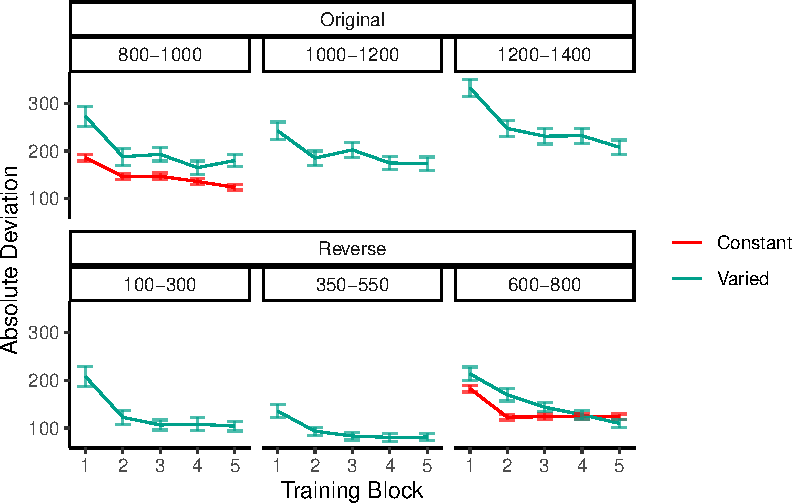
\includegraphics[keepaspectratio]{manuscript_files/figure-pdf/fig-e3-train-dev-1.pdf}}

}

\caption{\label{fig-e3-train-dev}Experiment 3 training. Deviations from
target band during training, shown separately for groups trained with
the original order (used in E1) and reverse order (used in E2).}

\end{figure}%

\begin{longtable}[]{@{}
  >{\raggedright\arraybackslash}p{(\linewidth - 8\tabcolsep) * \real{0.5354}}
  >{\raggedleft\arraybackslash}p{(\linewidth - 8\tabcolsep) * \real{0.1010}}
  >{\raggedleft\arraybackslash}p{(\linewidth - 8\tabcolsep) * \real{0.1515}}
  >{\raggedleft\arraybackslash}p{(\linewidth - 8\tabcolsep) * \real{0.1515}}
  >{\raggedleft\arraybackslash}p{(\linewidth - 8\tabcolsep) * \real{0.0606}}@{}}
\caption{\textbf{Experiment 3 testing accuracy}. Main effects of
condition and band type (training vs.~extrapolation), and the
interaction between the two factors. The Intercept represents the
baseline condition, (constant training, trained bands \& original
order), and the remaining coefficients reflect the deviation from that
baseline. Positive coefficients thus represent worse performance
relative to the baseline, and a positive interaction coefficient
indicates disproportionate deviation for the varied condition or reverse
order condition.}\label{tbl-e3-bmm-dist}\tabularnewline
\toprule\noalign{}
\begin{minipage}[b]{\linewidth}\raggedright
Term
\end{minipage} & \begin{minipage}[b]{\linewidth}\raggedleft
Estimate
\end{minipage} & \begin{minipage}[b]{\linewidth}\raggedleft
95\% CrI Lower
\end{minipage} & \begin{minipage}[b]{\linewidth}\raggedleft
95\% CrI Upper
\end{minipage} & \begin{minipage}[b]{\linewidth}\raggedleft
pd
\end{minipage} \\
\midrule\noalign{}
\endfirsthead
\toprule\noalign{}
\begin{minipage}[b]{\linewidth}\raggedright
Term
\end{minipage} & \begin{minipage}[b]{\linewidth}\raggedleft
Estimate
\end{minipage} & \begin{minipage}[b]{\linewidth}\raggedleft
95\% CrI Lower
\end{minipage} & \begin{minipage}[b]{\linewidth}\raggedleft
95\% CrI Upper
\end{minipage} & \begin{minipage}[b]{\linewidth}\raggedleft
pd
\end{minipage} \\
\midrule\noalign{}
\endhead
\bottomrule\noalign{}
\endlastfoot
Intercept & 288.65 & 199.45 & 374.07 & 1.00 \\
conditVaried & -40.19 & -104.68 & 23.13 & 0.89 \\
bandTypeExtrapolation & -23.35 & -57.28 & 10.35 & 0.92 \\
bandOrderReverse & -73.72 & -136.69 & -11.07 & 0.99 \\
\textbf{conditVaried:bandTypeExtrapolation} & 52.66 & 14.16 & 90.23 &
1.00 \\
conditVaried:bandOrderReverse & -37.48 & -123.28 & 49.37 & 0.80 \\
bandTypeExtrapolation:bandOrderReverse & 80.69 & 30.01 & 130.93 &
1.00 \\
conditVaried:bandTypeExtrapolation:bandOrder & 30.42 & -21.00 & 81.65 &
0.87 \\
\end{longtable}

\emph{Testing Accuracy.} Table~\ref{tbl-e3-bmm-dist} presents the
results of the Bayesian mixed effects model predicting absolute
deviation from the target band during the testing stage. There was no
significant main effect of training condition,\(\beta\) = -40.19, 95\%
CrI {[}-104.68, 23.13{]}; pd = 89.31\%, or band type,\(\beta\) = -23.35,
95\% CrI {[}-57.28, 10.35{]}; pd = 91.52\%. However the effect of band
order was significant, with the reverse order condition showing lower
deviations, \(\beta\) = -73.72, 95\% CrI {[}-136.69, -11.07{]}; pd =
98.89\%. The interaction between training condition and band type was
also significant \(\beta\) = 52.66, 95\% CrI {[}14.16, 90.23{]}; pd =
99.59\%, with the varied condition showing disproprionately large
deviations on the extrapolation bands compared to the constant group.
There was also a significant interaction between band type and band
order, \(\beta\) = 80.69, 95\% CrI {[}30.01, 130.93{]}; pd = 99.89\%,
such that the reverse order condition showed larger deviations on the
extrapolation bands. No other interactions were significant.

\begin{figure}

\centering{

\pandocbounded{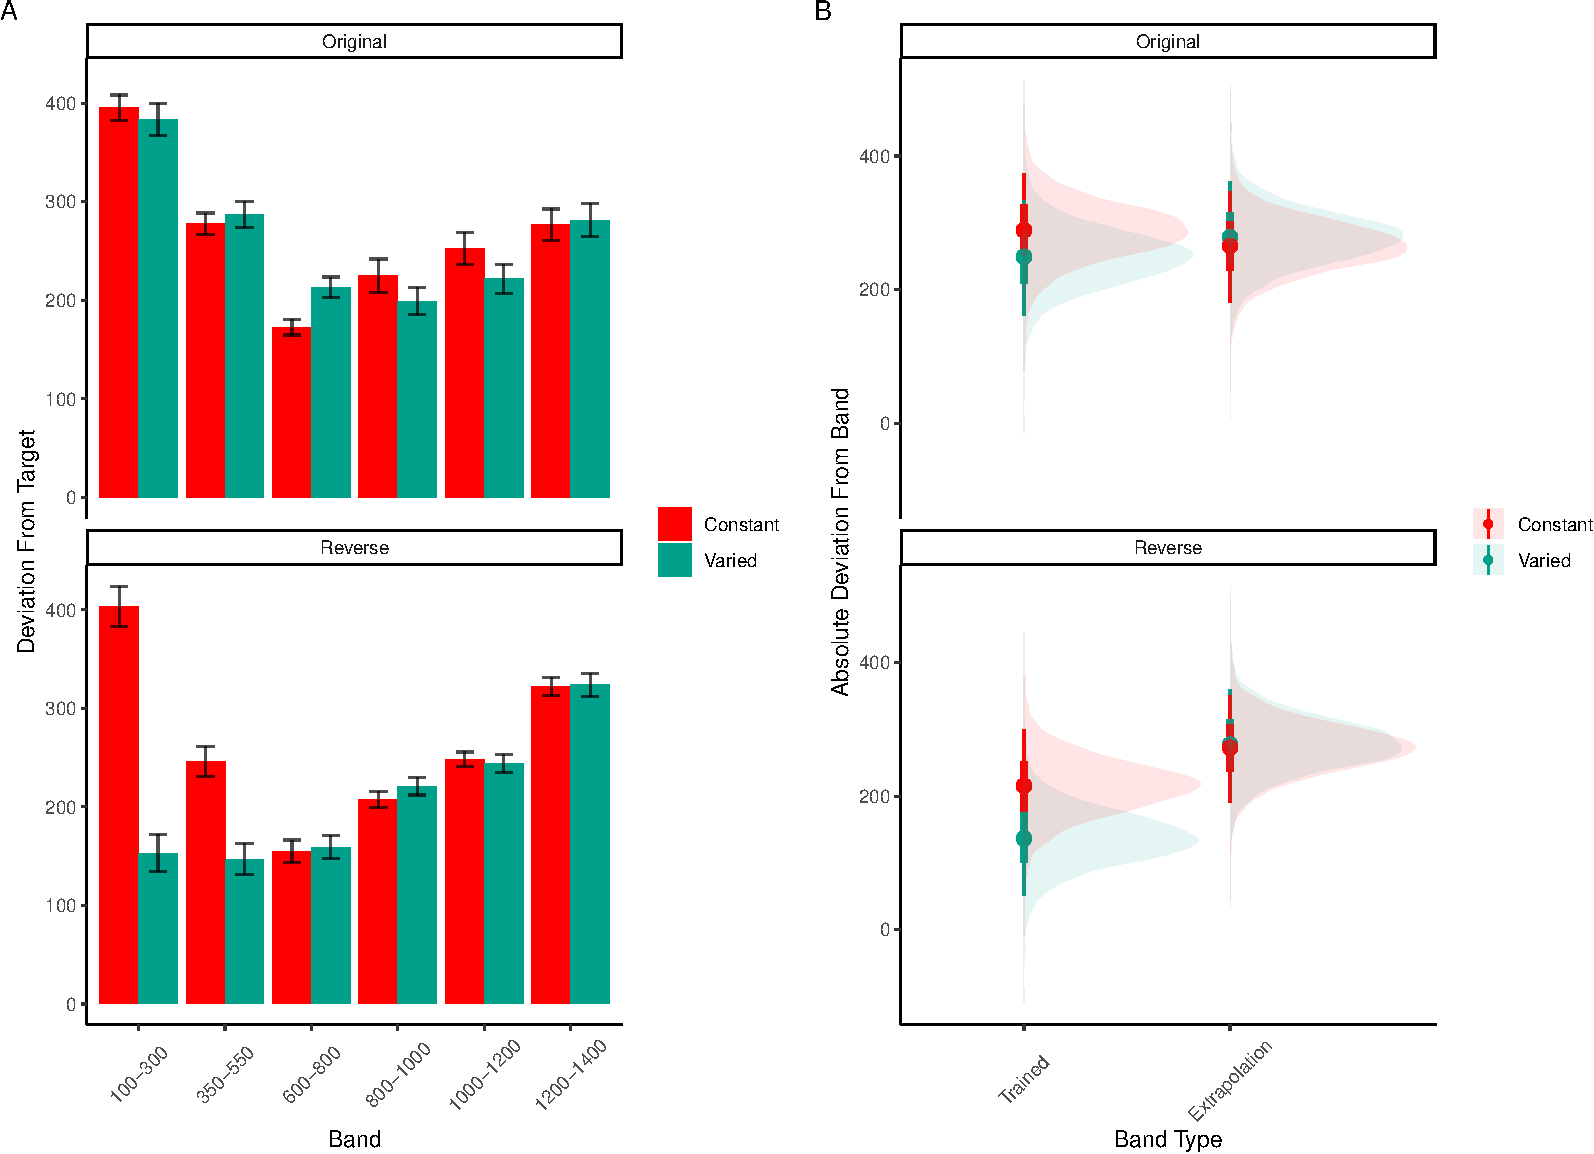
\includegraphics[keepaspectratio]{manuscript_files/figure-pdf/fig-e3-test-dev-1.pdf}}

}

\caption{\label{fig-e3-test-dev}Experiment 3 Testing Accuracy. A)
Empirical Deviations from target band during testing without feedback
stage. B) Conditional effect of condition (Constant vs.~Varied) and
testing band type (trained bands vs.~novel extrapolation bands) on
testing accuracy. Shown separately for groups trained with the original
order (used in E1) and reverse order (used in E2). Error bars represent
95\% credible intervals.}

\end{figure}%

\begin{longtable}[]{@{}
  >{\raggedright\arraybackslash}p{(\linewidth - 8\tabcolsep) * \real{0.4713}}
  >{\raggedleft\arraybackslash}p{(\linewidth - 8\tabcolsep) * \real{0.1149}}
  >{\raggedleft\arraybackslash}p{(\linewidth - 8\tabcolsep) * \real{0.1724}}
  >{\raggedleft\arraybackslash}p{(\linewidth - 8\tabcolsep) * \real{0.1724}}
  >{\raggedleft\arraybackslash}p{(\linewidth - 8\tabcolsep) * \real{0.0690}}@{}}
\caption{\textbf{Experiment 3 testing discrimination}. Bayesian Mixed
Model Predicting Vx as a function of condition (Constant vs.~Varied) and
Velocity Band. The Intercept represents the baseline condition (constant
training \& original order), and the Band coefficient represents the
slope for the baseline condition. The interaction terms which include
condit and Band (e.g., conditVaried:Band \&
conditVaried:bandOrderReverse:band) respectively indicate how the slopes
of the varied-original condition differed from the baseline condition,
and how varied-reverse condition differed from the varied-original
condition}\label{tbl-e3-bmm-vx}\tabularnewline
\toprule\noalign{}
\begin{minipage}[b]{\linewidth}\raggedright
Term
\end{minipage} & \begin{minipage}[b]{\linewidth}\raggedleft
Estimate
\end{minipage} & \begin{minipage}[b]{\linewidth}\raggedleft
95\% CrI Lower
\end{minipage} & \begin{minipage}[b]{\linewidth}\raggedleft
95\% CrI Upper
\end{minipage} & \begin{minipage}[b]{\linewidth}\raggedleft
pd
\end{minipage} \\
\midrule\noalign{}
\endfirsthead
\toprule\noalign{}
\begin{minipage}[b]{\linewidth}\raggedright
Term
\end{minipage} & \begin{minipage}[b]{\linewidth}\raggedleft
Estimate
\end{minipage} & \begin{minipage}[b]{\linewidth}\raggedleft
95\% CrI Lower
\end{minipage} & \begin{minipage}[b]{\linewidth}\raggedleft
95\% CrI Upper
\end{minipage} & \begin{minipage}[b]{\linewidth}\raggedleft
pd
\end{minipage} \\
\midrule\noalign{}
\endhead
\bottomrule\noalign{}
\endlastfoot
Intercept & 601.83 & 504.75 & 699.42 & 1.00 \\
conditVaried & 12.18 & -134.94 & 162.78 & 0.56 \\
bandOrderReverse & 13.03 & -123.89 & 144.67 & 0.58 \\
\textbf{Band} & 0.49 & 0.36 & 0.62 & 1.00 \\
\textbf{conditVaried:bandOrderReverse} & -338.15 & -541.44 & -132.58 &
1.00 \\
conditVaried:Band & -0.04 & -0.23 & 0.15 & 0.67 \\
bandOrderReverse:band & -0.10 & -0.27 & 0.08 & 0.86 \\
\textbf{conditVaried:bandOrderReverse:band} & 0.42 & 0.17 & 0.70 &
1.00 \\
\end{longtable}

\emph{Testing Discrimination.} The full results of the discrimination
model are presented in Table~\ref{tbl-e3-bmm-dist}. For the purposes of
assessing group differences in discrimination, only the coefficients
including the band variable are of interest. The baseline effect of band
represents the slope coefficient for the constant training - original
order condition, this effect was significant \(\beta\) = 0.49, 95\% CrI
{[}0.36, 0.62{]}; pd = 100\%. Neither of the two way interactions
reached significance, \(\beta\) = -0.04, 95\% CrI {[}-0.23, 0.15{]}; pd
= 66.63\%, \(\beta\) = -0.1, 95\% CrI {[}-0.27, 0.08{]}; pd = 86.35\%.
However, the three way interaction between training condition, band
order, and target band was significant, \(\beta\) = 0.42, 95\% CrI
{[}0.17, 0.7{]}; pd = 99.96\% - indicating a greater slope for the
varied condition trained with reverse order bands. This interaction is
shown in Figure~\ref{fig-e3-test-vx}, where the steepness of the best
fitting line for the varied-reversed condition is noticeably steeper
than the other conditions.

\begin{figure}

\centering{

\pandocbounded{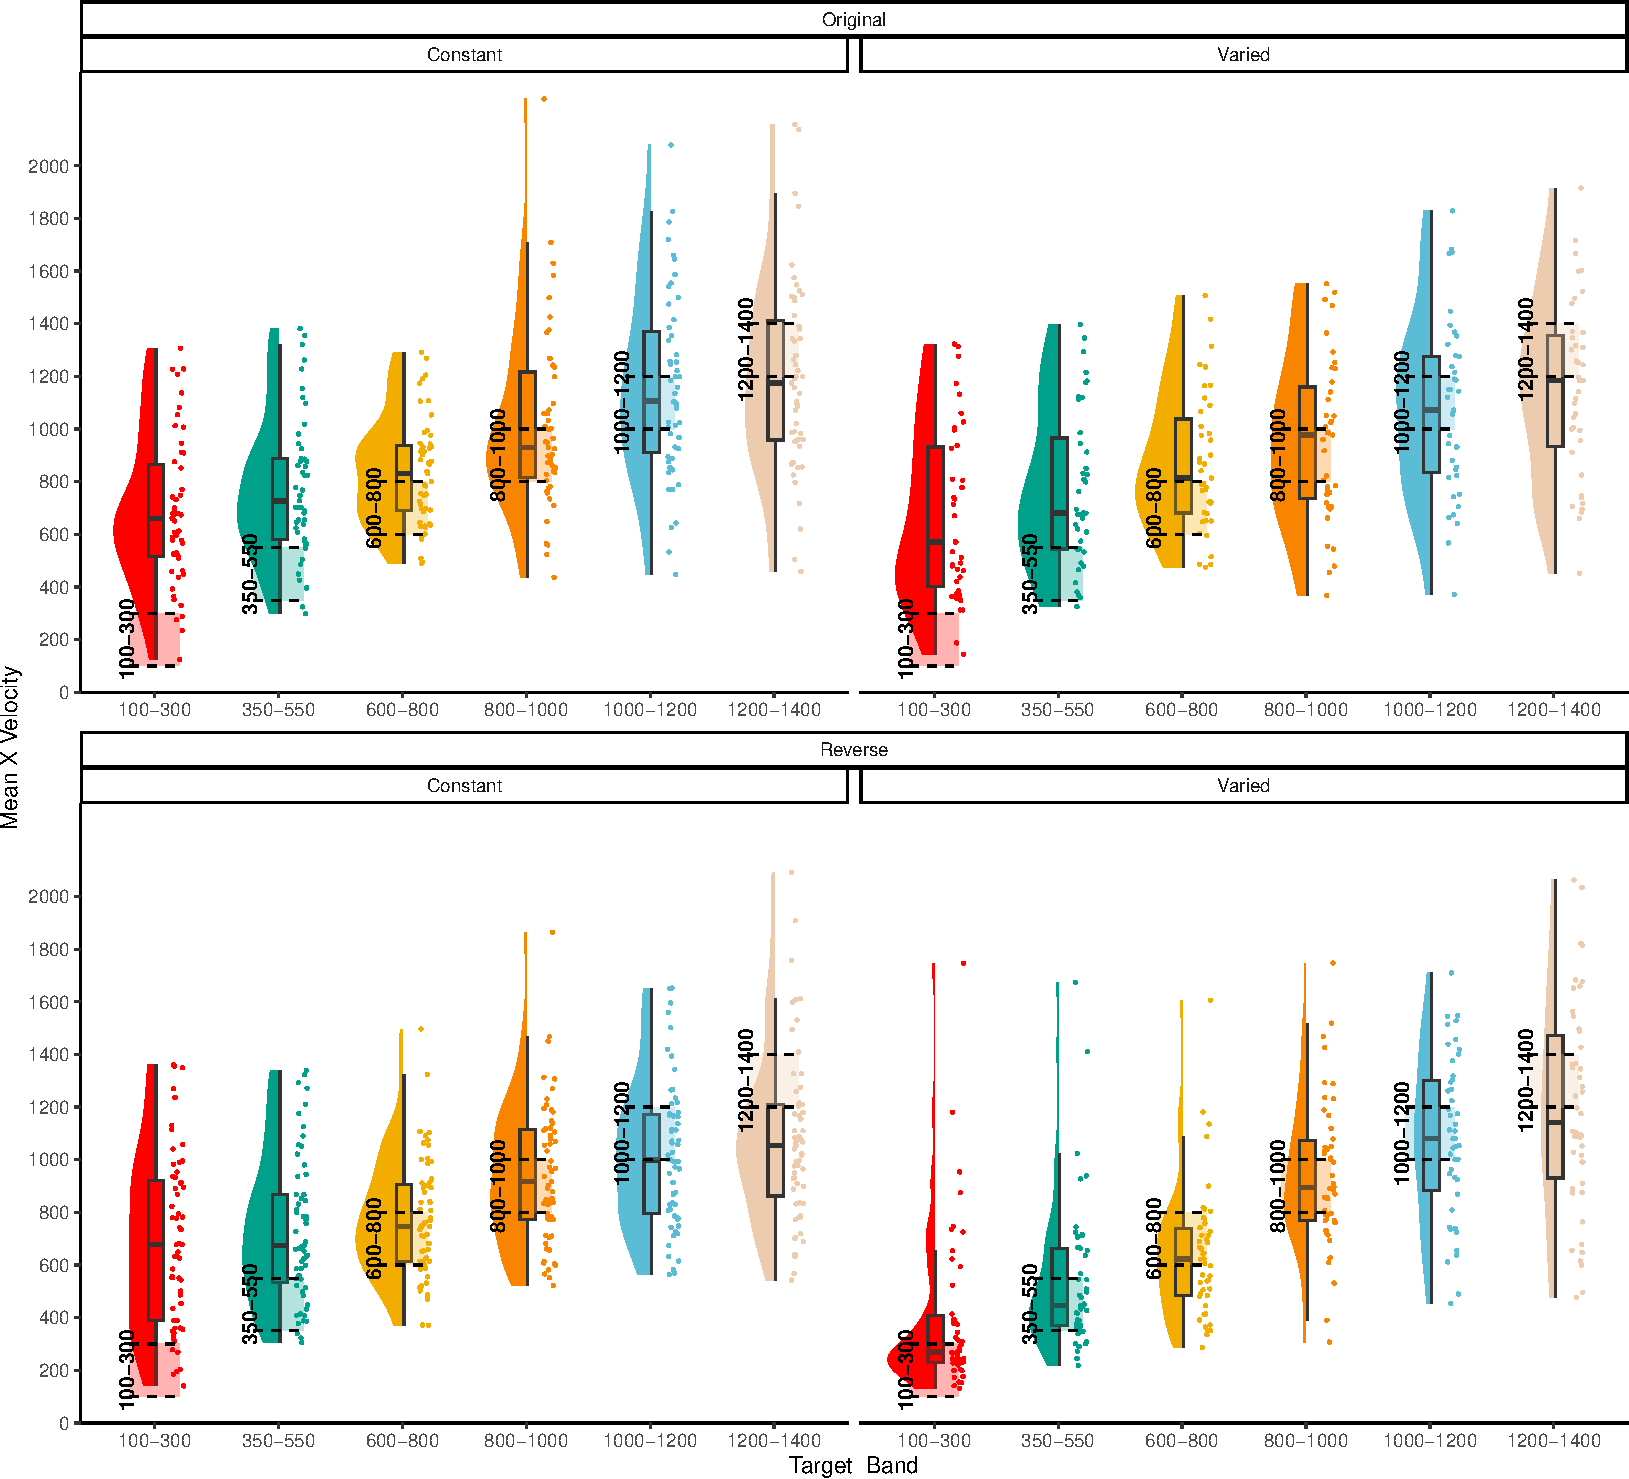
\includegraphics[keepaspectratio]{manuscript_files/figure-pdf/fig-e3-test-vx-1.pdf}}

}

\caption{\label{fig-e3-test-vx}Experiment 3. Empirical distribution of
velocities produced in the testing stage. Translucent bands with dash
lines indicate the correct range for each velocity band.}

\end{figure}%

\newpage{}

\begin{figure}

\centering{

\pandocbounded{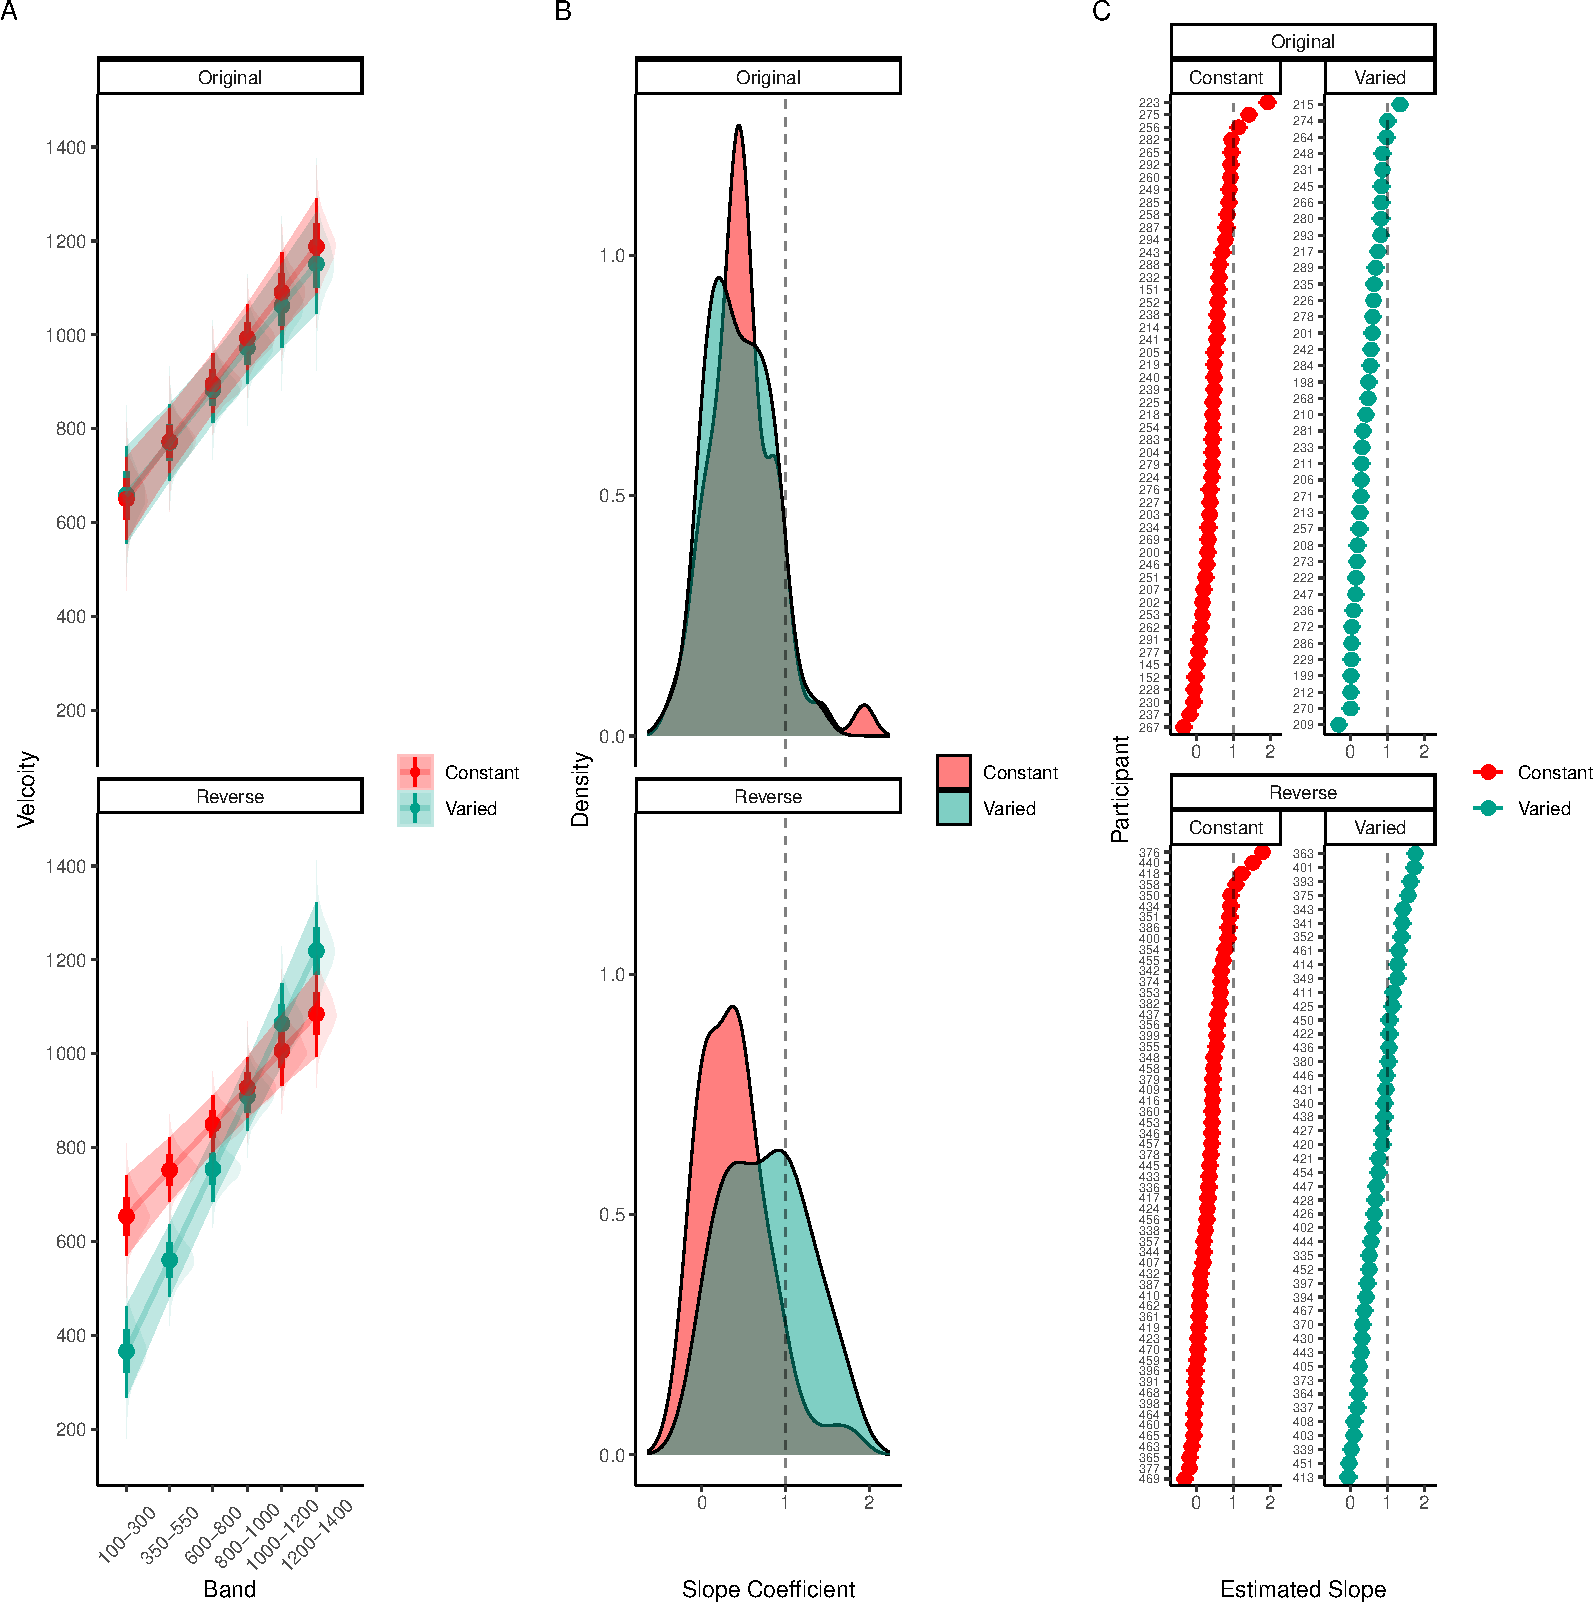
\includegraphics[keepaspectratio]{manuscript_files/figure-pdf/fig-e3-bmm-vx-1.pdf}}

}

\caption{\label{fig-e3-bmm-vx}Experiment 3 Discrimination. A)
Conditional effect of training condition and Band. Ribbons indicate 95\%
HDI. The steepness of the lines serves as an indicator of how well
participants discriminated between velocity bands. B) The distribution
of slope coefficients for each condition. Larger slopes indicate better
discrimination. C) Individual participant slopes. Error bars represent
95\% HDI.}

\end{figure}%

\subsubsection{Experiment 3 Summary}\label{experiment-3-summary}

In Experiment 3, we investigated the effects of training condition
(constant vs.~varied) and band type (training vs.~extrapolation) on
participants' accuracy and discrimination during the testing phase.
Unlike the previous experiments, participants received only ordinal, not
continuous valued, feedback during the training phase. Additionally,
Experiment 3 included both the original order condition from Experiment
1 and the reverse order condition from Experiment 2. The results
revealed no significant main effects of training condition on testing
accuracy, nor was there a significant difference between groups in band
discrimination. However, we observed a significant three-way interaction
for the discrimination analysis, indicating that the varied condition
showed a steeper slope coefficient on the reverse order bands compared
to the constant condition. This result suggests that varied training
enhanced participants' ability to discriminate between velocity bands,
but only when the band order was reversed during testing.

\subsection{Computational Model}\label{computational-model-1}

\begin{figure}

\centering{

\pandocbounded{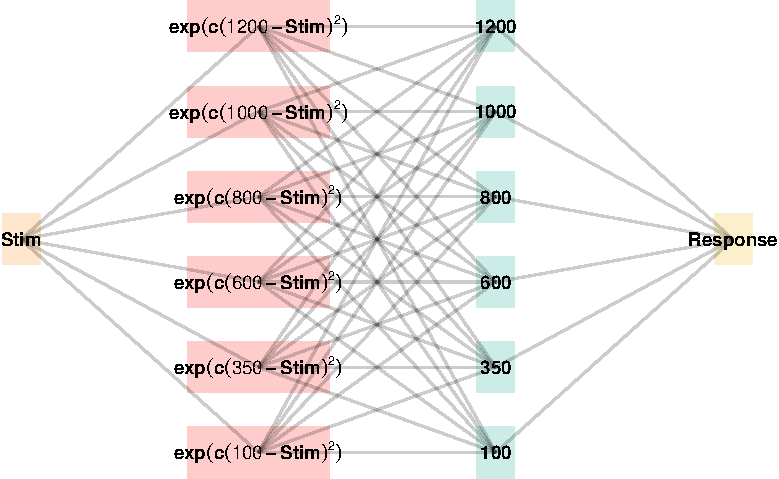
\includegraphics[keepaspectratio]{manuscript_files/figure-pdf/fig-alm-diagram-1.pdf}}

}

\caption{\label{fig-alm-diagram}The Associative Learning Model (ALM).
The diagram illustrates the basic structure of the ALM model used in the
present work. Input nodes are activated as a function of their
similarity to the lower-boundary of the target band. The generalization
parameter, \(c\), determines the degree to which nearby input nodes are
activated. The output nodes are activated as a function of the weighted
sum of the input nodes. During training, when feedback is provided,
network weights connecting the input layer to the output layer are
updated via the delta rule.}

\end{figure}%

The modeling goal is to implement a full process model capable of both
1) producing novel responses and 2) modeling behavior in both the
learning and testing stages of the experiment. For this purpose, we will
apply the associative learning model (ALM) and the EXAM model of
function learning (\citeproc{ref-deloshExtrapolationSineQua1997}{DeLosh
et al., 1997}). ALM is a simple connectionist learning model which
closely resembles Kruschke's ALCOVE model
(\citeproc{ref-kruschkeALCOVEExemplarbasedConnectionist1992}{Kruschke,
1992}), with modifications to allow for the generation of continuous
responses.

\subsubsection{ALM \& Exam}\label{alm-exam}

ALM is a localist neural network model
(\citeproc{ref-pageConnectionistModellingPsychology2000a}{Page, 2000}),
with each input node corresponding to a particular stimulus, and each
output node corresponding to a particular response value. The units in
the input layer activate as a function of their Gaussian similarity to
the input stimulus ( a\_i(X) = exp(-c(X - X\_i)\^{}2) ). So, for
example, an input stimulus of value 55 would induce maximal activation
of the input unit tuned to 55. Depending on the value of the
generalization parameter, the nearby units (e.g., 54 and 56; 53 and 57)
may also activate to some degree. The units in the input layer activate
as a function of their similarity to a presented stimulus. The input
layer is fully connected to the output layer, and the activation for any
particular output node is simply the weighted sum of the connection
weights between that node and the input activations. The network then
produces a response by taking the weighted average of the output units
(recall that each output unit has a value corresponding to a particular
response). During training, the network receives feedback which
activates each output unit as a function of its distance from the ideal
level of activation necessary to produce the correct response. The
connection weights between input and output units are then updated via
the standard delta learning rule, where the magnitude of weight changes
are controlled by a learning rate parameter.

The EXAM model is an extension of ALM, with the same learning rule and
representational scheme for input and output units. EXAM differs from
ALM only in its response rule, as it includes a linear extrapolation
mechanism for generating novel responses. When a novel test stimulus,
\(X\), is presented, EXAM first identifies the two nearest training
stimuli, \(X_1\) and \(X_2\), that bracket \(X\). This is done based on
the Gaussian activation of input nodes, similar to ALM, but focuses on
identifying the closest known points for extrapolation.

\textbf{Slope Calculation}: EXAM calculates a local slope, \(S\), using
the responses associated with \(X_1\) and \(X_2\). This is computed as:

\[
   S = \frac{m(X_{1}) - m(X_{2})}{X_{1} - X_{2}}
   \]

where \(m(X_1)\) and \(m(X_2)\) are the output values from ALM
corresponding to the \(X_1\) and \(X_2\) inputs.

\textbf{Response Generation}: The response for the novel stimulus \(X\)
is then extrapolated using the slope \(S\):

\[
   E[Y|X] = m(X_1) + S \cdot |X - X_1|
   \]

Here, \(m(X_1)\) is the ALM response value from the training data for
the stimulus closest to \(X\), and \((X - X_1)\) represents the distance
between the novel stimulus and the nearest training stimulus.

Although this extrapolation rule departs from a strictly
similarity-based generalization mechanism, EXAM is distinct from pure
rule-based models in that it remains constrained by the weights learned
during training. EXAM retrieves the two nearest training inputs, and the
ALM responses associated with those inputs, and computes the slope
between these two points. The slope is then used to extrapolate the
response to the novel test stimulus. Because EXAM requires at least two
input-output pairs to generate a response, additional assumptions were
required in order for it to generate resposnes for the constant group.
We assumed that participants come to the task with prior knowledge of
the origin point (0,0), which can serve as a reference point necessary
for the model to generate responses for the constant group. This
assumption is motivated by previous function learning research
(\citeproc{ref-brownUnderestimationLinearFunction2017}{Brown \& Lacroix,
2017}), which through a series of manipulations of the y intercept of
the underlying function, found that participants consistently
demonstrated knowledge of, or a bias towards, the origin point (see
Kwantes \& Neal (\citeproc{ref-kwantesWhyPeopleUnderestimate2006}{2006})
for additional evidence of such a bias in function learning tasks).

See Table~\ref{tbl-alm-exam} for a full specification of the equations
that define ALM and EXAM, and Figure~\ref{fig-alm-diagram} for a visual
representation of the ALM model.

\begin{longtable}[]{@{}
  >{\raggedright\arraybackslash}p{(\linewidth - 4\tabcolsep) * \real{0.2500}}
  >{\raggedright\arraybackslash}p{(\linewidth - 4\tabcolsep) * \real{0.4028}}
  >{\raggedright\arraybackslash}p{(\linewidth - 4\tabcolsep) * \real{0.3472}}@{}}
\caption{ALM \& EXAM Equations}\label{tbl-alm-exam}\tabularnewline
\toprule\noalign{}
\begin{minipage}[b]{\linewidth}\raggedright
\end{minipage} & \begin{minipage}[b]{\linewidth}\raggedright
\textbf{ALM Response Generation}
\end{minipage} & \begin{minipage}[b]{\linewidth}\raggedright
\end{minipage} \\
\midrule\noalign{}
\endfirsthead
\toprule\noalign{}
\begin{minipage}[b]{\linewidth}\raggedright
\end{minipage} & \begin{minipage}[b]{\linewidth}\raggedright
\textbf{ALM Response Generation}
\end{minipage} & \begin{minipage}[b]{\linewidth}\raggedright
\end{minipage} \\
\midrule\noalign{}
\endhead
\bottomrule\noalign{}
\endlastfoot
Input Activation &
\(a_i(X) = \frac{e^{-c(X-X_i)^2}}{\sum_{k=1}^M e^{-c(X-X_k)^2}}\) &
Input nodes activate as a function of Gaussian similarity to stimulus \\
Output Activation & \(O_j(X) = \sum_{k=1}^M w_{ji} \cdot a_i(X)\) &
Output unit \(O_j\) activation is the weighted sum of input activations
and association weights \\
Output Probability & \(P[Y_j|X] = \frac{O_j(X)}{\sum_{k=1}^M O_k(X)}\) &
The response, \(Y_j\) probabilites computed via Luce's choice rule \\
Mean Output &
\(m(X) = \sum_{j=1}^L Y_j \cdot \frac{O_j(x)}{\sum_{k=1}^M O_k(X)}\) &
Weighted average of probabilities determines response to X \\
& \textbf{ALM Learning} & \\
Feedback & \(f_j(Z) = e^{-c(Z-Y_j)^2}\) & feedback signal Z computed as
similarity between ideal response and observed response \\
magnitude of error & \(\Delta_{ji}=(f_{j}(Z)-o_{j}(X))a_{i}(X)\) & Delta
rule to update weights. \\
Update Weights & \(w_{ji}^{new}=w_{ji}+\eta\Delta_{ji}\) & Updates
scaled by learning rate parameter \(\eta\). \\
& \textbf{EXAM Extrapolation} & \\
Instance Retrieval & \(P[X_i|X] = \frac{a_i(X)}{\sum_{k=1}^M a_k(X)}\) &
Novel test stimulus \(X\) activates input nodes \(X_i\) \\
Slope Computation & \(S =\) \(\frac{m(X_{1})-m(X_{2})}{X_{1}-X_{2}}\) &
Slope value, \(S\) computed from nearest training instances \\
Response & \(E[Y|X_i] = m(X_i) + S \cdot [X - X_i]\) & Final EXAM
response is the ALM response for the nearest training stimulus,
\(m(X_i)\), adjusted by local slope \(S\). \\
\end{longtable}

\subsubsection{Model Fitting}\label{model-fitting}

To fit ALM and EXAM to our participant data, we employ a similar method
to McDaniel et al.
(\citeproc{ref-mcdanielPredictingTransferPerformance2009}{2009}),
wherein we examine the performance of each model after being fit to
various subsets of the data. Each model was fit to the data with three
separate procedures: 1) fit to maximize predictions of the testing data,
2) fit to maximize predictions of both the training and testing data, 3)
fit to maximize predictions of the just the training data. We refer to
this fitting manipulations as ``Fit Method'' in the tables and figures
below. It should be emphasized that for all three fit methods, the ALM
and EXAM models behave identically - with weights updating only during
the training phase. Models were fit separately to the data of each
individual participant. The free parameters for both models are the
generalization (\(c\)) and learning rate (\(lr\)) parameters. Parameter
estimation was performed using approximate Bayesian computation (ABC),
which we describe in detail below.

\begin{tcolorbox}[enhanced jigsaw, opacityback=0, left=2mm, colframe=quarto-callout-color-frame, toprule=.15mm, rightrule=.15mm, leftrule=.75mm, bottomrule=.15mm, arc=.35mm, breakable, colback=white]

\textbf{\faIcon{lightbulb} Approximate Bayesian Computation}

To estimate the parameters of ALM and EXAM, we used approximate Bayesian
computation (ABC), enabling us to obtain an estimate of the posterior
distribution of the generalization and learning rate parameters for each
individual. ABC belongs to the class of simulation-based inference
methods
(\citeproc{ref-cranmerFrontierSimulationbasedInference2020}{Cranmer et
al., 2020}), which have begun being used for parameter estimation in
cognitive modeling relatively recently
(\citeproc{ref-kangasraasioParameterInferenceComputational2019}{Kangasrääsiö
et al., 2019};
\citeproc{ref-turnerBayesianAnalysisSimulationbased2016}{Turner et al.,
2016}; \citeproc{ref-turnerTutorialApproximateBayesian2012}{Turner \&
Van Zandt, 2012}). Although they can be applied to any model from which
data can be simulated, ABC methods are most useful for complex models
that lack an explicit likelihood function (e.g., many neural network
models).

The general ABC procedure is to 1) define a prior distribution over
model parameters. 2) sample candidate parameter values, \(\theta^*\),
from the prior. 3) Use \(\theta^*\) to generate a simulated dataset,
\(Data_{sim}\). 4) Compute a measure of discrepancy between the
simulated and observed datasets, \(discrep\)(\(Data_{sim}\),
\(Data_{obs}\)). 5) Accept \(\theta^*\) if the discrepancy is less than
the tolerance threshold, \(\epsilon\), otherwise reject \(\theta^*\). 6)
Repeat until the desired number of posterior samples are obtained.

Although simple in the abstract, implementations of ABC require
researchers to make a number of non-trivial decisions as to i) the
discrepancy function between observed and simulated data, ii) whether to
compute the discrepancy between trial level data, or a summary statistic
of the datasets, iii) the value of the minimum tolerance \(\epsilon\)
between simulated and observed data. For the present work, we follow the
guidelines from previously published ABC tutorials
(\citeproc{ref-farrellComputationalModelingCognition2018}{Farrell \&
Lewandowsky, 2018};
\citeproc{ref-turnerTutorialApproximateBayesian2012}{Turner \& Van
Zandt, 2012}). For the test stage, we summarized datasets with mean
velocity of each band in the observed dataset as \(V_{obs}^{(k)}\) and
in the simulated dataset as \(V_{sim}^{(k)}\), where \(k\) represents
each of the six velocity bands. For computing the discrepancy between
datasets in the training stage, we aggregated training trials into three
equally sized blocks (separately for each velocity band in the case of
the varied group). After obtaining the summary statistics of the
simulated and observed datasets, the discrepancy was computed as the
mean of the absolute difference between simulated and observed datasets
(Equation~\ref{eq-discrep-test} and Equation~\ref{eq-discrep-train}).
For the models fit to both training and testing data, discrepancies were
computed for both stages, and then averaged together.

\begin{equation}\phantomsection\label{eq-discrep-test}{
discrep_{Test}(Data_{sim}, Data_{obs}) = \frac{1}{6} \sum_{k=1}^{6} |V_{obs}^{(k)} - V_{sim}^{(k)}|
}\end{equation}

\begin{equation}\phantomsection\label{eq-discrep-train}{
\begin{aligned} \\
discrep_{Train,constant}(Data_{sim}, Data_{obs}) = \frac{1}{N_{blocks}} \sum_{j=1}^{N_{blocks}} |V_{obs,constant}^{(j)} - V_{sim,constant}^{(j)}| \\ \\
discrep_{Train,varied}(Data_{sim}, Data_{obs}) = \frac{1}{N_{blocks} \times 3} \sum_{j=1}^{N_{blocks}} \sum_{k=1}^{3} |V_{obs,varied}^{(j,k)} - V_{sim,varied}^{(j,k)}|
\end{aligned}
}\end{equation}

The final component of our ABC implementation is the determination of an
appropriate value of \(\epsilon\). The setting of \(\epsilon\) exerts
strong influence on the approximated posterior distribution. Smaller
values of \(\epsilon\) increase the rejection rate, and improve the
fidelity of the approximated posterior, while larger values result in an
ABC sampler that simply reproduces the prior distribution. Because the
individual participants in our dataset differed substantially in terms
of the noisiness of their data, we employed an adaptive tolerance
setting strategy to tailor \(\epsilon\) to each individual. The initial
value of \(\epsilon\) was set to the overall standard deviation of each
individual's velocity values. Thus, sampled parameter values that
generated simulated data within a standard deviation of the observed
data were accepted, while worse performing parameters were rejected.
After every 300 samples the tolerance was allowed to increase only if
the current acceptance rate of the algorithm was less than 1\%. In such
cases, the tolerance was shifted towards the average discrepancy of the
5 best samples obtained thus far. To ensure the acceptance rate did not
become overly permissive, \(\epsilon\) was also allowed to decrease
every time a sample was accepted into the posterior.

\end{tcolorbox}

For each of the 156 participants from Experiment 1, the ABC algorithm
was run until 200 samples of parameters were accepted into the posterior
distribution. Obtaining this number of posterior samples required an
average of 205,000 simulation runs per participant. Fitting each
combination of participant, Model (EXAM \& ALM), and fitting method
(Test only, Train only, Test \& Train) required a total of 192 million
simulation runs. To facilitate these intensive computational demands, we
used the Future Package in R
(\citeproc{ref-bengtssonUnifyingFrameworkParallel2021}{Bengtsson,
2021}), allowing us to parallelize computations across a cluster of ten
M1 iMacs, each with 8 cores.

\subsubsection{Modelling Results}\label{modelling-results}

\begingroup
\fontsize{9.0pt}{10.8pt}\selectfont

\begin{longtable}{lcrrrr}

\caption{\label{tbl-htw-modelError-e1}Model errors predicting empirical
data from Experiment 1 - aggregated over the full posterior distribution
for each participant. Note that Fit Method refers to the subset of the
data that the model was trained on, while Task Stage refers to the
subset of the data that the model was evaluated on.}

\tabularnewline

\toprule
 &  & \multicolumn{2}{c}{ALM} & \multicolumn{2}{c}{EXAM} \\ 
\cmidrule(lr){3-4} \cmidrule(lr){5-6}
{Task Stage} & {Fit Method} & Constant & Varied & Constant & Varied \\ 
\midrule\addlinespace[2.5pt]
{\cellcolor[HTML]{FFFFFF}{Test}} & {\cellcolor[HTML]{FFFFFF}{Fit to Test Data}} & {\cellcolor[HTML]{FFFFFF}{199.93}} & {\cellcolor[HTML]{FFFFFF}{103.36}} & {\cellcolor[HTML]{FFFFFF}{104.01}} & {\cellcolor[HTML]{FFFFFF}{85.68}} \\ 
{\cellcolor[HTML]{FFFFFF}{Test}} & {\cellcolor[HTML]{FFFFFF}{Fit to Test \& Training Data}} & {\cellcolor[HTML]{FFFFFF}{216.97}} & {\cellcolor[HTML]{FFFFFF}{170.28}} & {\cellcolor[HTML]{FFFFFF}{127.94}} & {\cellcolor[HTML]{FFFFFF}{144.86}} \\ 
{\cellcolor[HTML]{FFFFFF}{Test}} & {\cellcolor[HTML]{FFFFFF}{Fit to Training Data}} & {\cellcolor[HTML]{FFFFFF}{467.73}} & {\cellcolor[HTML]{FFFFFF}{291.38}} & {\cellcolor[HTML]{FFFFFF}{273.30}} & {\cellcolor[HTML]{FFFFFF}{297.91}} \\ 
{\cellcolor[HTML]{FFFFFF}{Train}} & {\cellcolor[HTML]{FFFFFF}{Fit to Test Data}} & {\cellcolor[HTML]{FFFFFF}{297.82}} & {\cellcolor[HTML]{FFFFFF}{2,016.01}} & {\cellcolor[HTML]{FFFFFF}{53.90}} & {\cellcolor[HTML]{FFFFFF}{184.00}} \\ 
{\cellcolor[HTML]{FFFFFF}{Train}} & {\cellcolor[HTML]{FFFFFF}{Fit to Test \& Training Data}} & {\cellcolor[HTML]{FFFFFF}{57.40}} & {\cellcolor[HTML]{FFFFFF}{132.32}} & {\cellcolor[HTML]{FFFFFF}{42.92}} & {\cellcolor[HTML]{FFFFFF}{127.90}} \\ 
{\cellcolor[HTML]{FFFFFF}{Train}} & {\cellcolor[HTML]{FFFFFF}{Fit to Training Data}} & {\cellcolor[HTML]{FFFFFF}{51.77}} & {\cellcolor[HTML]{FFFFFF}{103.48}} & {\cellcolor[HTML]{FFFFFF}{51.43}} & {\cellcolor[HTML]{FFFFFF}{107.03}} \\ 
\bottomrule

\end{longtable}

\endgroup

\begin{figure}

\centering{

\pandocbounded{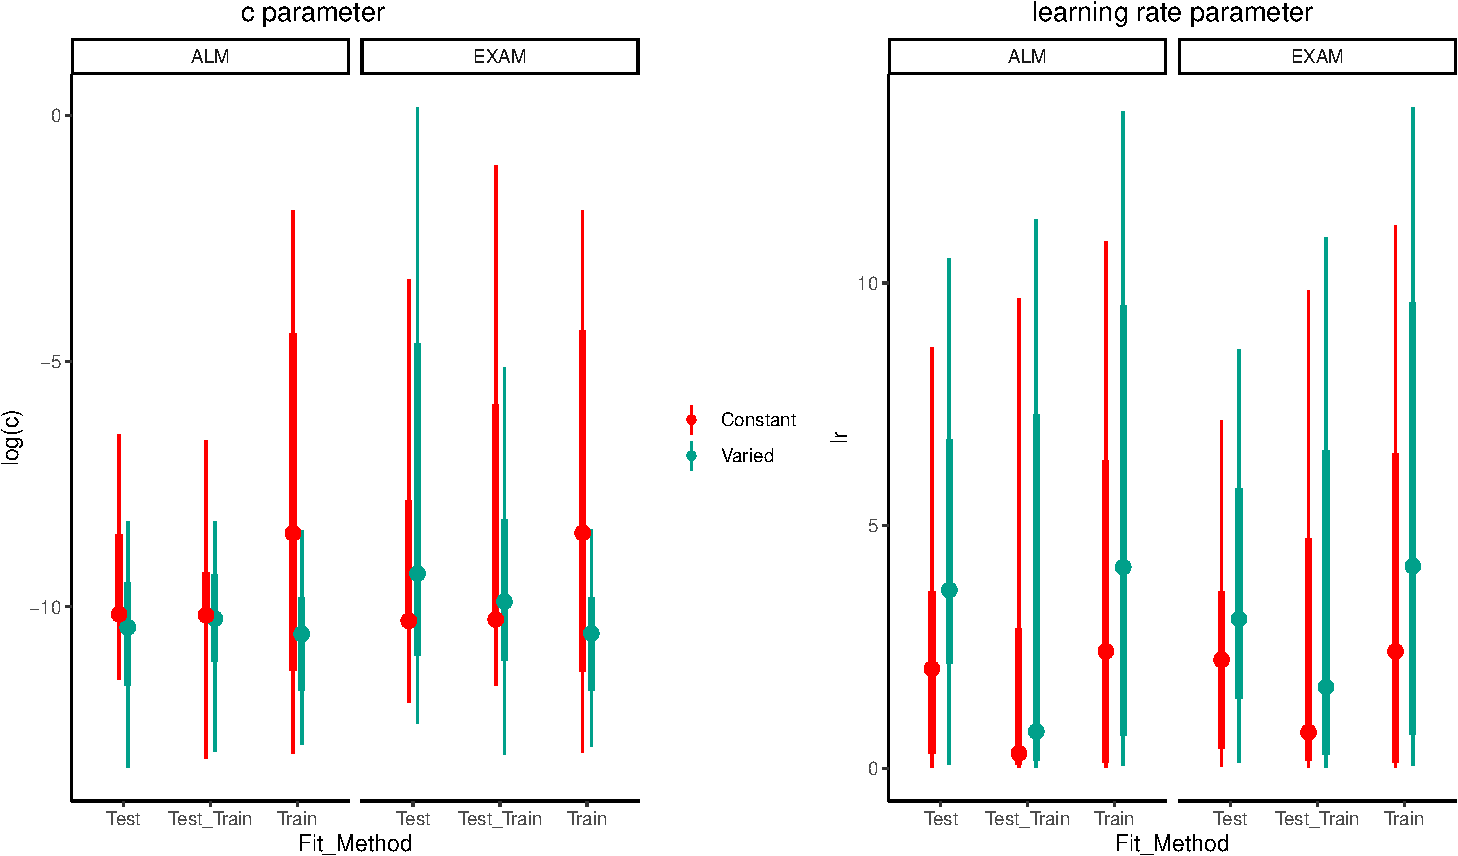
\includegraphics[keepaspectratio]{manuscript_files/figure-pdf/fig-htw-post-dist-1.pdf}}

}

\caption{\label{fig-htw-post-dist}Posterior Distributions of \(c\) and
\(lr\) parameters. Points represent median values, thicker intervals
represent 66\% credible intervals and thin intervals represent 95\%
credible intervals around the median. Note that the y-axes of the plots
for the \(c\) parameter are scaled logarithmically.}

\end{figure}%

\begin{figure}

\centering{

\pandocbounded{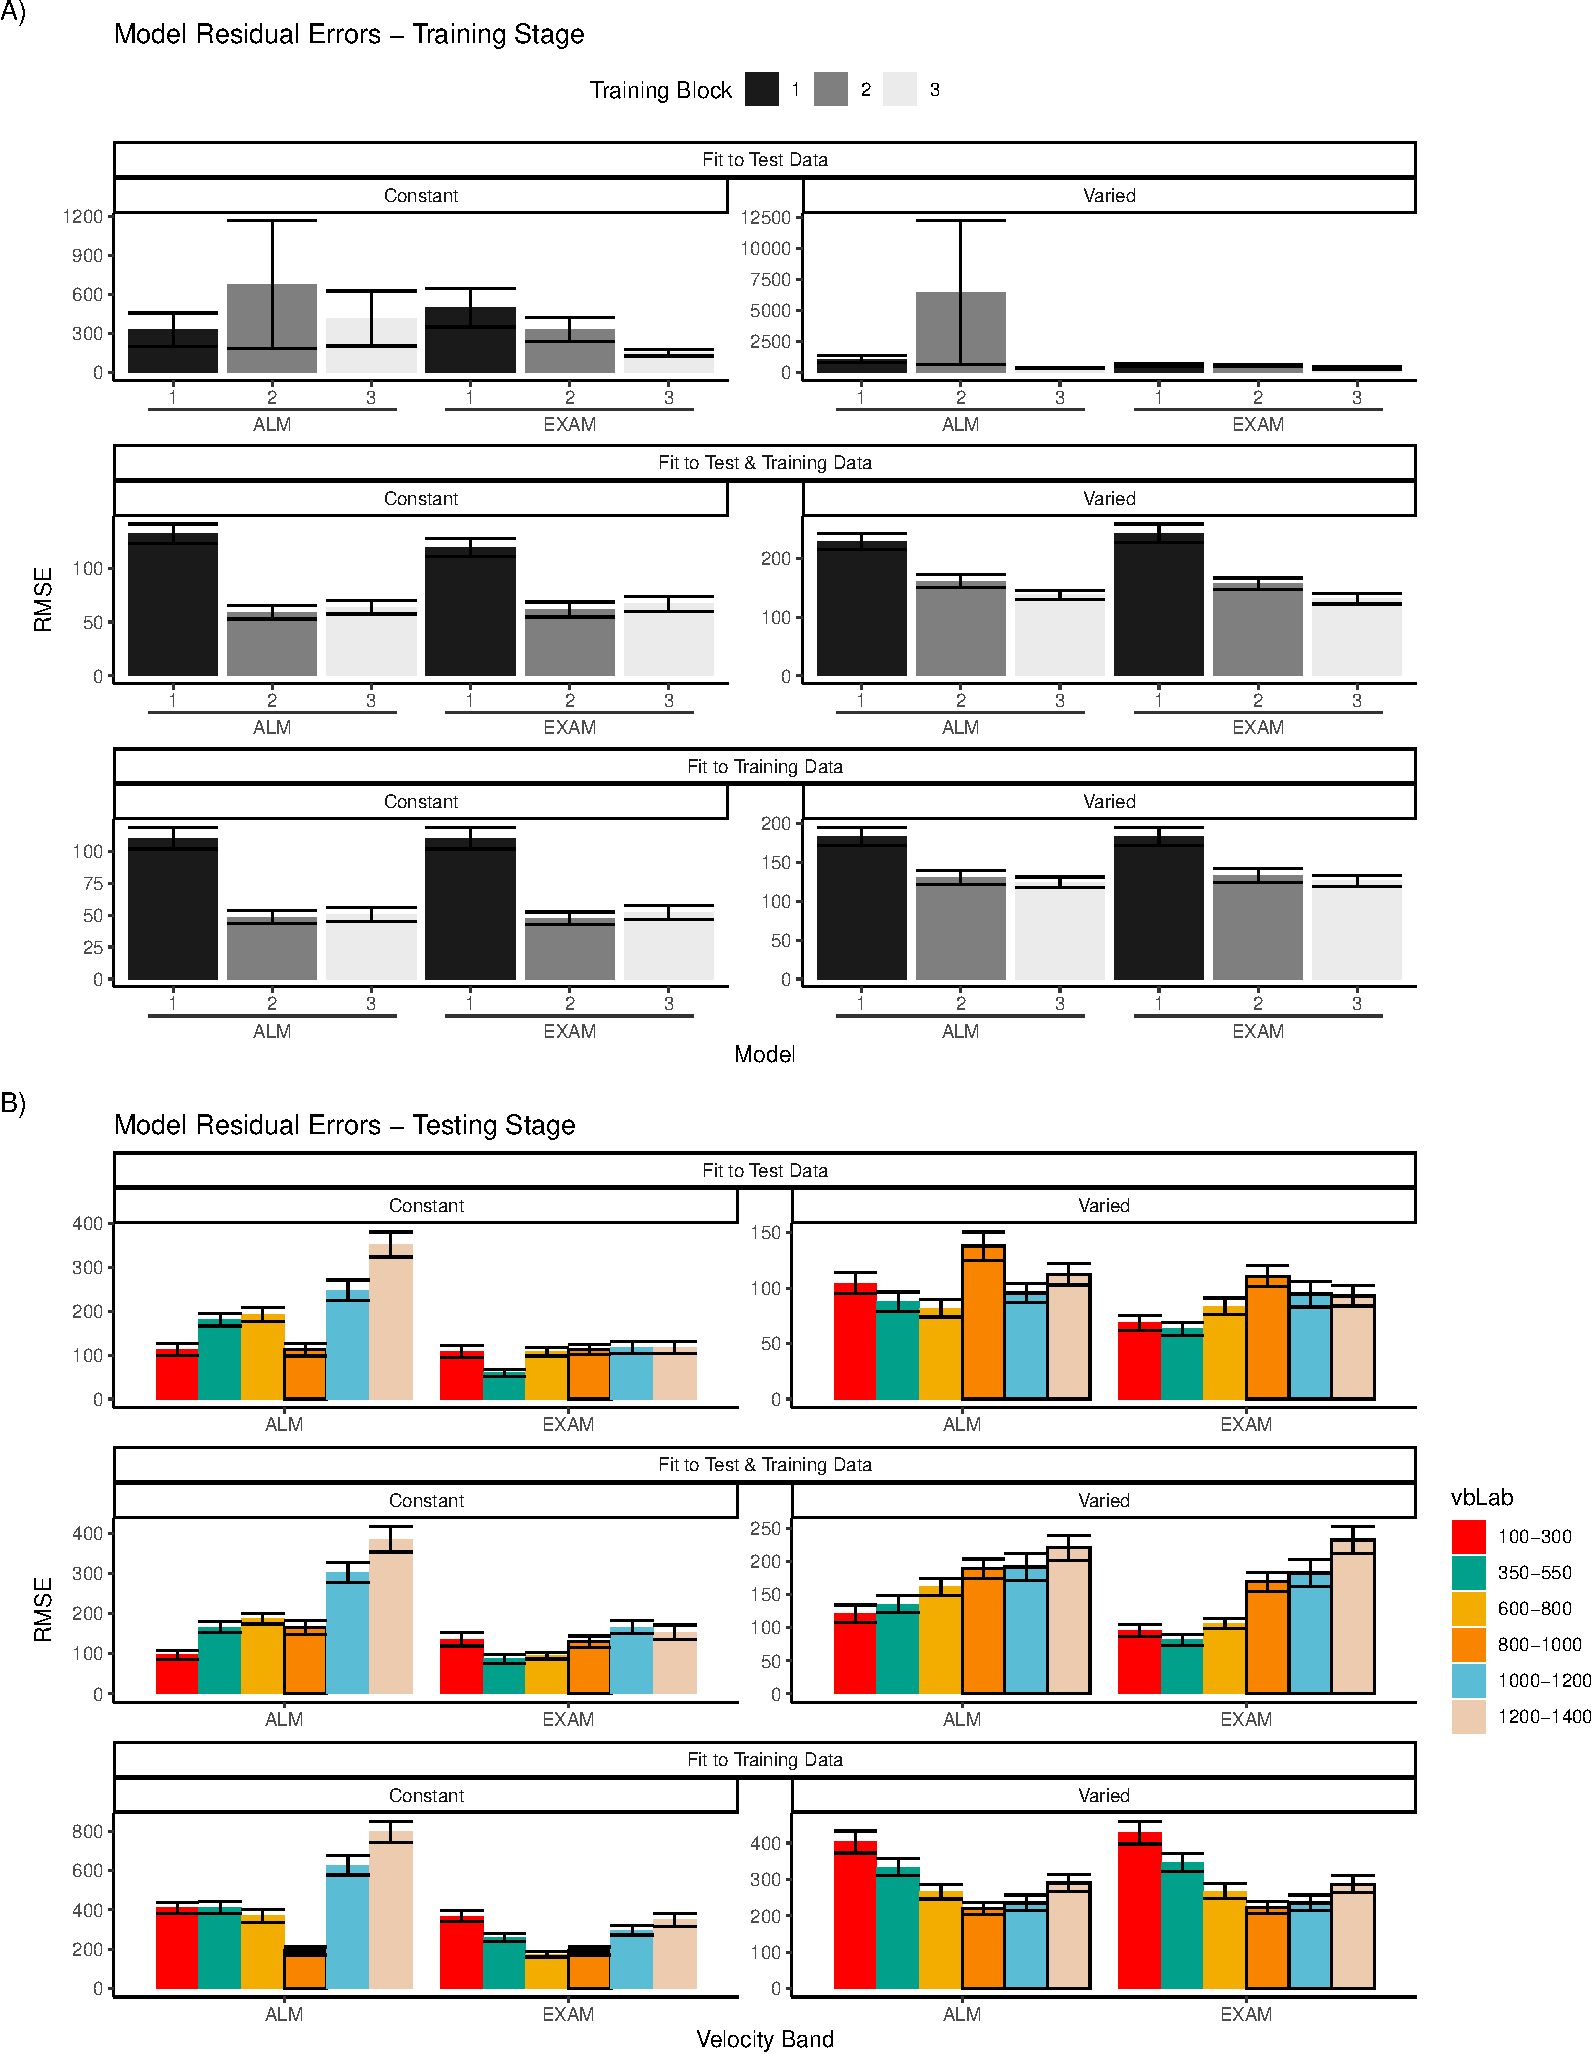
\includegraphics[keepaspectratio]{manuscript_files/figure-pdf/fig-htw-resid-pred-1.pdf}}

}

\caption{\label{fig-htw-resid-pred}Model residuals for each combination
of training condition, fit method, and model. Residuals reflect the
difference between observed and predicted values. Lower values indicate
better model fit. Note that y-axes are scaled differently between
facets. A) Residuals predicting each block of the training data. B)
Residuals predicting each band during the testing stage. Bolded bars
indicate bands that were trained, non-bold bars indicate extrapolation
bands.}

\end{figure}%

The posterior distributions of the \(c\) and \(lr\) parameters are shown
Figure~\ref{fig-htw-post-dist}, and model predictions are shown
alongside the empirical data in Figure~\ref{fig-cm-vx-pat}. There were
substantial individual differences in the posteriors of both parameters,
with the within-group individual differences generally swamped any
between-group or between-model differences. The magnitude of these
individual differences remains even if we consider only the single best
parameter set for each subject.

We used the posterior distribution of \(c\) and \(lr\) parameters to
generate a posterior predictive distribution of the observed data for
each participant, which then allows us to compare the empirical data to
the full range of predictions from each model. Aggregated residuals are
displayed in Figure~\ref{fig-htw-resid-pred}. The pattern of training
stage residual errors are unsurprising across the combinations of models
and fitting method . Differences in training performance between ALM and
EXAM are generally minor (the two models have identical learning
mechanisms). The differences in the magnitude of residuals across the
three fitting methods are also straightforward, with massive errors for
the `fit to Test Only' model, and the smallest errors for the `fit to
train only' models. It is also noteworthy that the residual errors are
generally larger for the first block of training, which is likely due to
the initial values of the ALM weights being unconstrained by whatever
initial biases participants tend to bring to the task. Future work may
explore the ability of the models to capture more fine grained aspects
of the learning trajectories. However for the present purposes, our
primary interest is in the ability of ALM and EXAM to account for the
testing patterns while being constrained, or not constrained, by the
training data. All subsequent analyses and discussion will thus focus on
the testing stage.

The residuals of the model predictions for the testing stage
(Figure~\ref{fig-htw-resid-pred}) show an unsurprising pattern across
fitting methods - with models fit only to the test data showing the best
performance, followed by models fit to both training and test data, and
with models fit only to the training data showing the worst performance
(note that Y-axes are scaled different between plots). Although EXAM
tends to perform better for both Constant and Varied participants (see
also Figure~\ref{fig-ee-e1}), the relative advantage of EXAM is
generally larger for the Constant group - a pattern consistent across
all three fitting methods. The primary predictive difference between ALM
and EXAM is made clear in Figure~\ref{fig-cm-vx-pat}, which directly
compares the observed data against the posterior predictive
distributions for both models. Regardless of how the models are fit,
only EXAM can capture the pattern where participants are able to
discriminate all 6 target bands.

\begin{figure}

\centering{

\pandocbounded{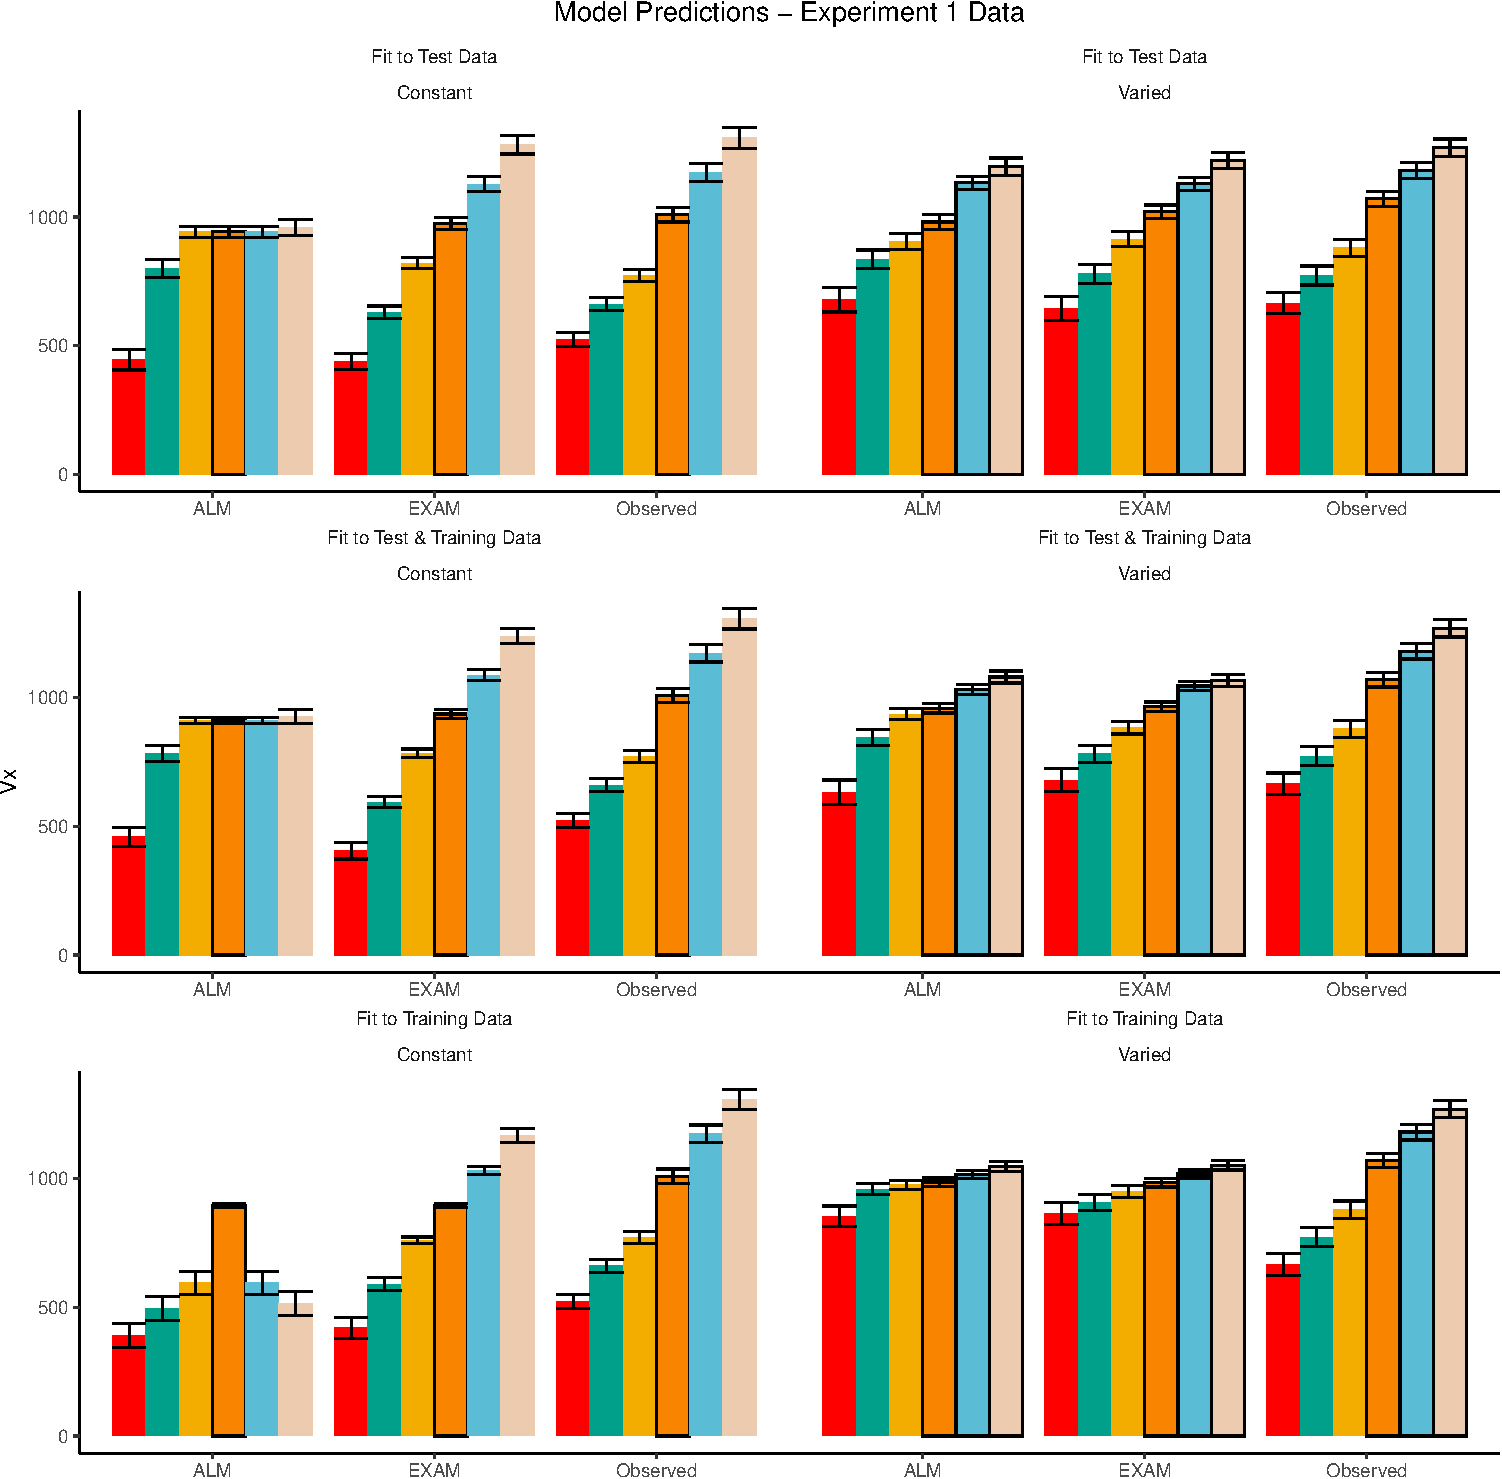
\includegraphics[keepaspectratio]{manuscript_files/figure-pdf/fig-cm-vx-pat-1.pdf}}

}

\caption{\label{fig-cm-vx-pat}Empirical data and Model predictions for
mean velocity across target bands. Fitting methods (Test Only, Test \&
Train, Train Only) - are separated across rows, and Training Condition
(Constant vs.~Varied) are separated by columns. Each facet contains the
predictions of ALM and EXAM, alongside the observed data.}

\end{figure}%

\begin{figure}

\centering{

\pandocbounded{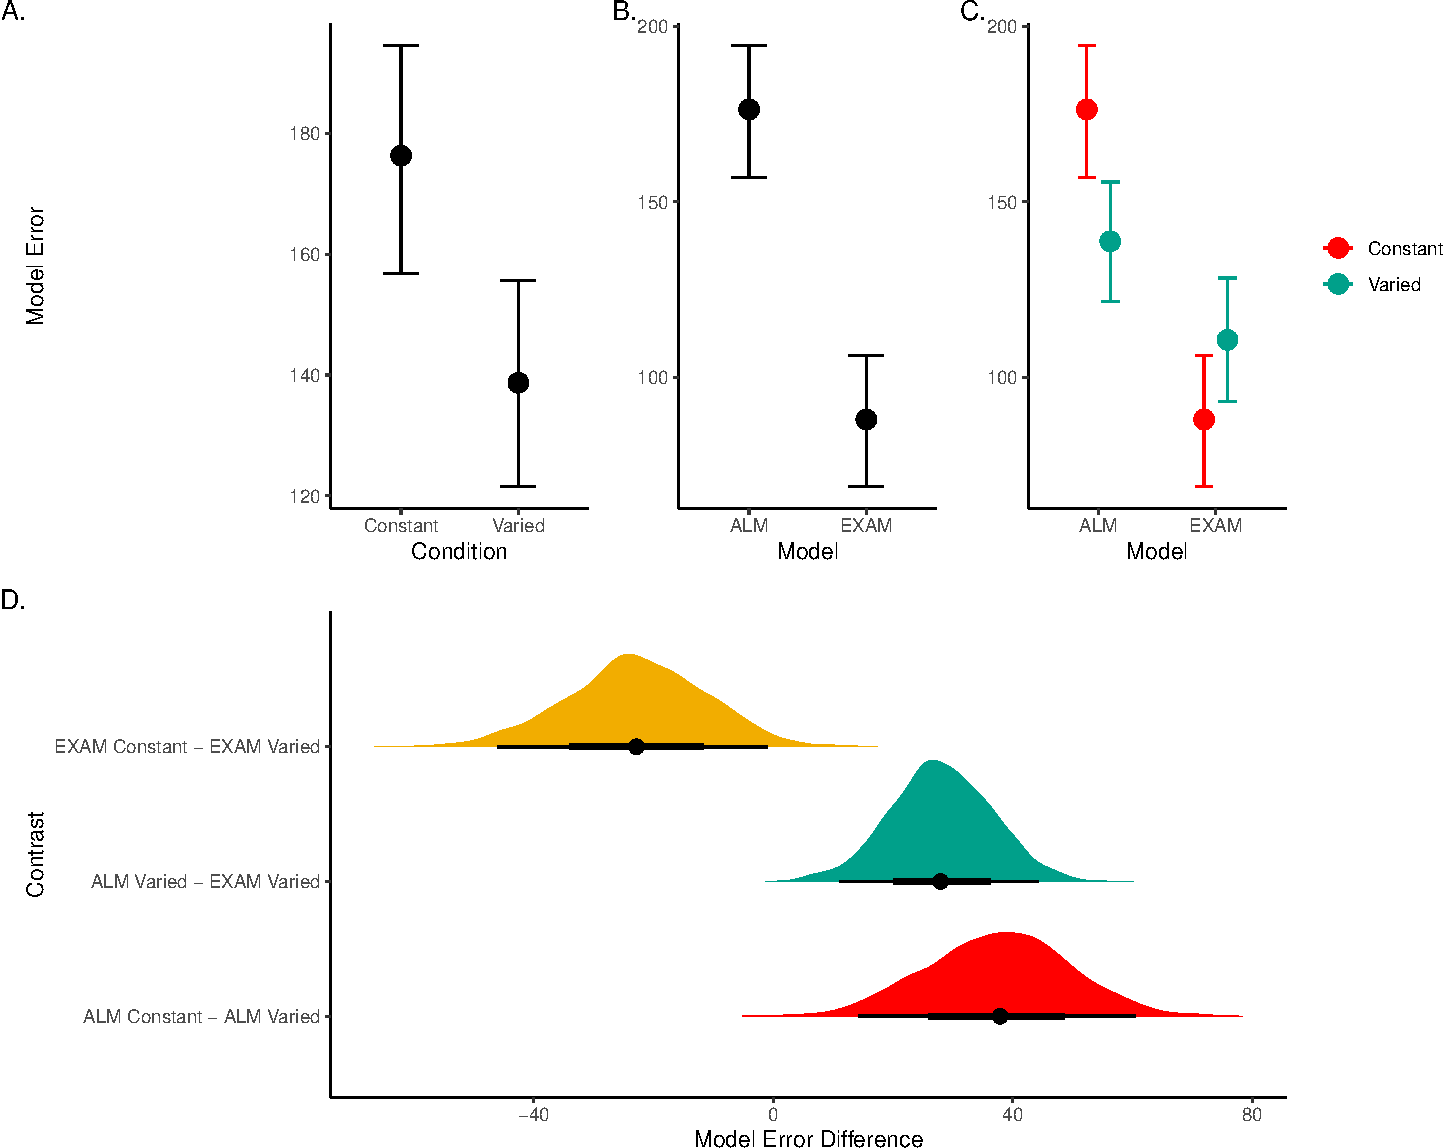
\includegraphics[keepaspectratio]{manuscript_files/figure-pdf/fig-ee-e1-1.pdf}}

}

\caption{\label{fig-ee-e1}A-C) Conditional effects of Model (ALM vs
EXAM) and Condition (Constant vs.~Varied). Lower values on the y axis
indicate better model fit. D) Specific contrasts of model performance
comparing 1) EXAM fits between constant and varied training; 2) ALM
vs.~EXAM for the varied group; 3) ALM fits between constant and varied.
Negative error differences indicate that the term on the left side
(e.g., EXAM Constant) tended to have smaller model residuals.}

\end{figure}%

To quantitatively assess the differences in performance between models,
we fit a Bayesian regression model predicting the errors of the
posterior predictions of each model as a function of the Model (ALM
vs.~EXAM) and training condition (Constant vs.~Varied).

Model errors were significantly lower for EXAM (\(\beta\) = -37.54, 95\%
CrI {[}-60.4, -14.17{]}, pd = 99.85\%) than ALM. There was also a
significant interaction between Model and Condition (\(\beta\) = 60.42,
95\% CrI {[}36.17, 83.85{]}, pd = 100\%), indicating that the advantage
of EXAM over ALM was significantly greater for the constant group. To
assess whether EXAM predicts performance significantly better for
Constant than for Varied subjects, we calculated the difference in model
error between the Constant and Varied conditions specifically for EXAM.
The results indicated that the model error for EXAM was significantly
lower in the Constant condition compared to the Varied condition, with a
mean difference of -22.88 (95\% CrI {[}-46.02, -0.97{]}, pd = 0.98).

\begingroup
\fontsize{9.0pt}{10.8pt}\selectfont

\begin{longtable}{lrrrrrrrr}

\caption{\label{tbl-htw-modelError-e23}Models errors predicting
empirical data - aggregated over all participants, posterior parameter
values, and velocity bands. Note that Fit Method refers to the subset of
the data that the model was trained on, while Task Stage refers to the
subset of the data that the model was evaluated on.}

\tabularnewline

\toprule
 & \multicolumn{4}{c}{E2} & \multicolumn{4}{c}{E3} \\ 
\cmidrule(lr){2-5} \cmidrule(lr){6-9}
 & \multicolumn{2}{c}{ALM} & \multicolumn{2}{c}{EXAM} & \multicolumn{2}{c}{ALM} & \multicolumn{2}{c}{EXAM} \\ 
\cmidrule(lr){2-3} \cmidrule(lr){4-5} \cmidrule(lr){6-7} \cmidrule(lr){8-9}
Task Stage & Constant & Varied & Constant & Varied & Constant & Varied & Constant & Varied \\ 
\midrule\addlinespace[2.5pt]
\multicolumn{9}{l}{Fit to Test Data} \\[2.5pt] 
\midrule\addlinespace[2.5pt]
{\cellcolor[HTML]{FFFFFF}{Test}} & {\cellcolor[HTML]{FFFFFF}{239.7}} & {\cellcolor[HTML]{FFFFFF}{129.8}} & {\cellcolor[HTML]{FFFFFF}{99.7}} & {\cellcolor[HTML]{FFFFFF}{88.2}} & {\cellcolor[HTML]{FFFFFF}{170.1}} & {\cellcolor[HTML]{FFFFFF}{106.1}} & {\cellcolor[HTML]{FFFFFF}{92.3}} & {\cellcolor[HTML]{FFFFFF}{72.8}} \\ 
{\cellcolor[HTML]{FFFFFF}{Train}} & {\cellcolor[HTML]{FFFFFF}{53.1}} & {\cellcolor[HTML]{FFFFFF}{527.1}} & {\cellcolor[HTML]{FFFFFF}{108.1}} & {\cellcolor[HTML]{FFFFFF}{169.3}} & {\cellcolor[HTML]{FFFFFF}{70.9}} & {\cellcolor[HTML]{FFFFFF}{543.5}} & {\cellcolor[HTML]{FFFFFF}{157.8}} & {\cellcolor[HTML]{FFFFFF}{212.7}} \\ 
\midrule\addlinespace[2.5pt]
\multicolumn{9}{l}{Fit to Test \& Training Data} \\[2.5pt] 
\midrule\addlinespace[2.5pt]
{\cellcolor[HTML]{FFFFFF}{Test}} & {\cellcolor[HTML]{FFFFFF}{266.0}} & {\cellcolor[HTML]{FFFFFF}{208.2}} & {\cellcolor[HTML]{FFFFFF}{125.1}} & {\cellcolor[HTML]{FFFFFF}{126.4}} & {\cellcolor[HTML]{FFFFFF}{197.7}} & {\cellcolor[HTML]{FFFFFF}{189.5}} & {\cellcolor[HTML]{FFFFFF}{130.0}} & {\cellcolor[HTML]{FFFFFF}{128.5}} \\ 
{\cellcolor[HTML]{FFFFFF}{Train}} & {\cellcolor[HTML]{FFFFFF}{40.0}} & {\cellcolor[HTML]{FFFFFF}{35.4}} & {\cellcolor[HTML]{FFFFFF}{30.4}} & {\cellcolor[HTML]{FFFFFF}{23.6}} & {\cellcolor[HTML]{FFFFFF}{49.1}} & {\cellcolor[HTML]{FFFFFF}{85.6}} & {\cellcolor[HTML]{FFFFFF}{49.2}} & {\cellcolor[HTML]{FFFFFF}{78.4}} \\ 
\midrule\addlinespace[2.5pt]
\multicolumn{9}{l}{Fit to Training Data} \\[2.5pt] 
\midrule\addlinespace[2.5pt]
{\cellcolor[HTML]{FFFFFF}{Test}} & {\cellcolor[HTML]{FFFFFF}{357.4}} & {\cellcolor[HTML]{FFFFFF}{295.9}} & {\cellcolor[HTML]{FFFFFF}{305.1}} & {\cellcolor[HTML]{FFFFFF}{234.5}} & {\cellcolor[HTML]{FFFFFF}{415.0}} & {\cellcolor[HTML]{FFFFFF}{298.8}} & {\cellcolor[HTML]{FFFFFF}{295.5}} & {\cellcolor[HTML]{FFFFFF}{243.7}} \\ 
{\cellcolor[HTML]{FFFFFF}{Train}} & {\cellcolor[HTML]{FFFFFF}{42.5}} & {\cellcolor[HTML]{FFFFFF}{23.0}} & {\cellcolor[HTML]{FFFFFF}{43.2}} & {\cellcolor[HTML]{FFFFFF}{22.6}} & {\cellcolor[HTML]{FFFFFF}{51.4}} & {\cellcolor[HTML]{FFFFFF}{63.8}} & {\cellcolor[HTML]{FFFFFF}{51.8}} & {\cellcolor[HTML]{FFFFFF}{65.3}} \\ 
\bottomrule

\end{longtable}

\endgroup

\begin{figure}

\centering{

\pandocbounded{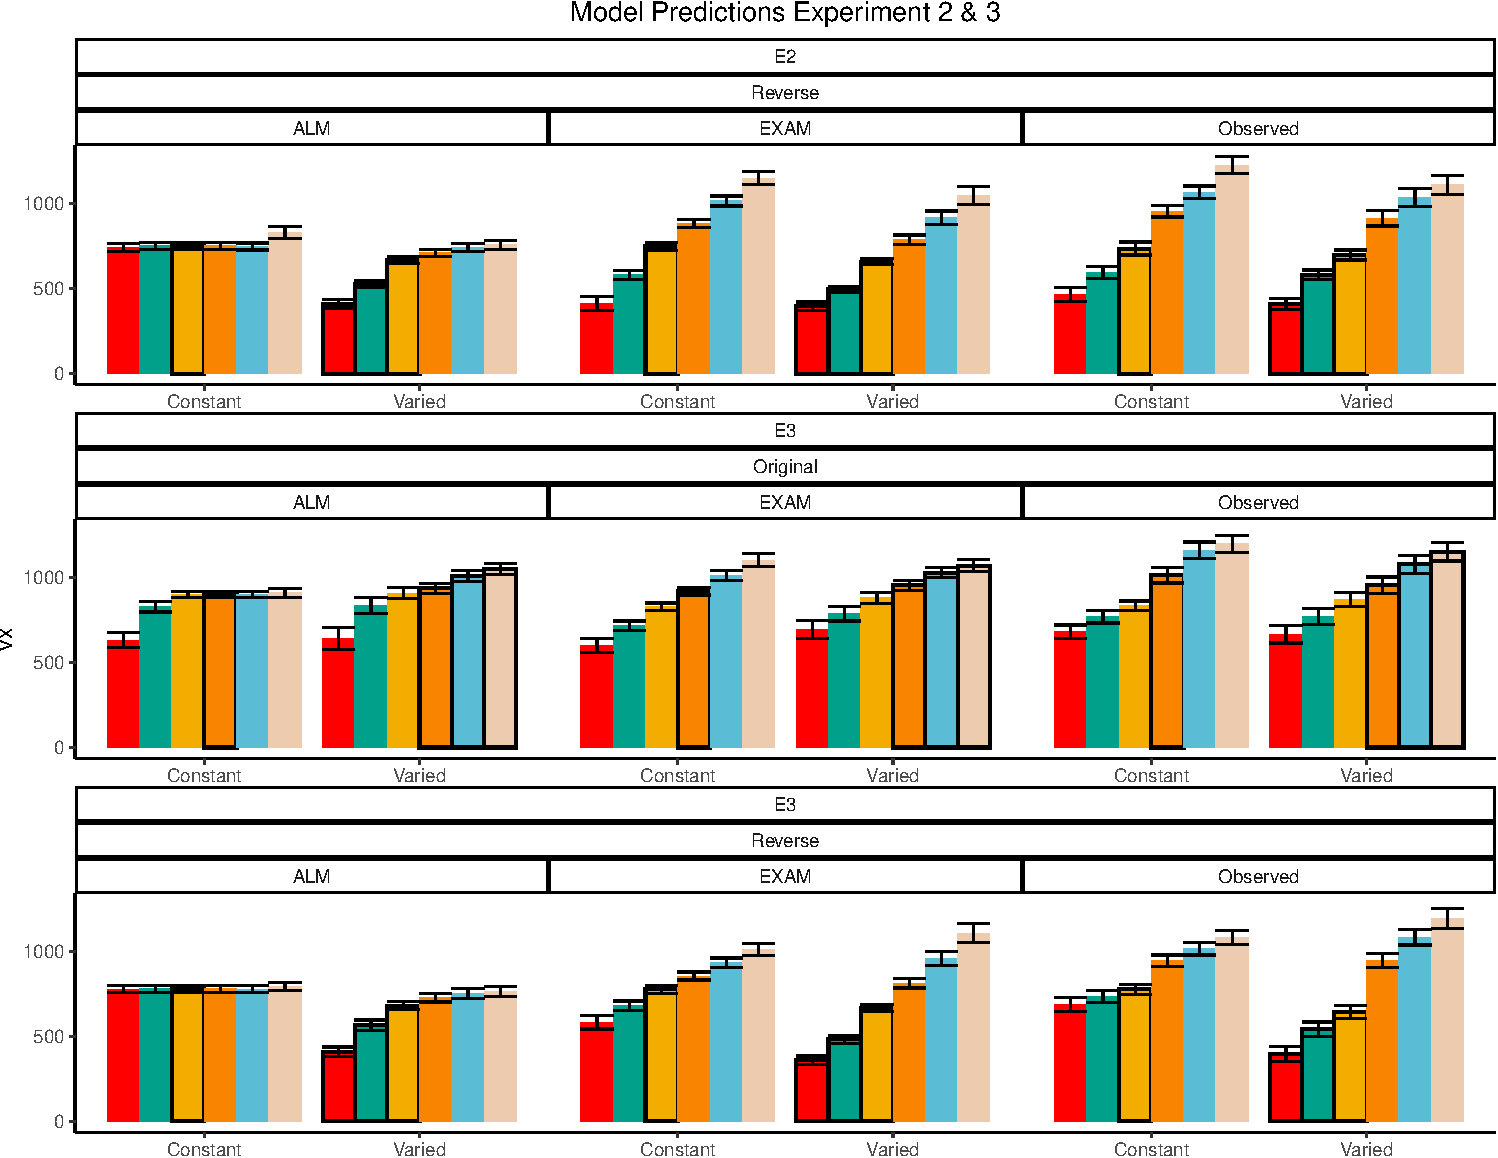
\includegraphics[keepaspectratio]{manuscript_files/figure-pdf/fig-cm-vx-pat-e2-e3-1.pdf}}

}

\caption{\label{fig-cm-vx-pat-e2-e3}Empirical data and Model predictions
from Experiment 2 and 3 for the testing stage. Observed data is shown on
the right. Bolded bars indicate bands that were trained, non-bold bars
indicate extrapolation bands.}

\end{figure}%

\newpage{}

\scriptsize

\begingroup
\fontsize{9.0pt}{10.8pt}\selectfont

\begin{longtable}{llrrrr}

\caption{\label{tbl-htw-ee-e23}Results of Bayesian Regression models
predicting model error as a function of Model (ALM vs.~EXAM), Condition
(Constant vs.~Varied), and the interaction between Model and Condition.
The values represent the estimated coefficient for each term, with 95\%
credible intervals in brackets. The intercept reflects the baseline of
ALM and Constant. The other estimates indicate deviations from the
baseline for the EXAM mode and varied condition. Lower values indicate
better model fit.}

\tabularnewline

\toprule
 &  &  & \multicolumn{2}{c}{Credible Interval} &  \\ 
\cmidrule(lr){4-5}
Experiment & Term & Estimate & 95\% CrI Lower & 95\% CrI Upper & pd \\ 
\midrule\addlinespace[2.5pt]
\multicolumn{6}{l}{Experiment 1} \\[2.5pt] 
\midrule\addlinespace[2.5pt]
Exp 1 & Intercept & 176.3 & 156.9 & 194.6 & 1.00 \\ 
Exp 1 & ModelEXAM & -88.4 & -104.5 & -71.8 & 1.00 \\ 
Exp 1 & conditVaried & -37.5 & -60.4 & -14.2 & 1.00 \\ 
Exp 1 & ModelEXAM:conditVaried & {\bfseries \cellcolor[HTML]{FFFFFF}{60.4}} & 36.2 & 83.8 & {\bfseries \cellcolor[HTML]{FFFFFF}{1.00}} \\ 
\midrule\addlinespace[2.5pt]
\multicolumn{6}{l}{Experiment 2} \\[2.5pt] 
\midrule\addlinespace[2.5pt]
Exp 2 & Intercept & 245.9 & 226.2 & 264.5 & 1.00 \\ 
Exp 2 & ModelEXAM & -137.7 & -160.2 & -115.5 & 1.00 \\ 
Exp 2 & conditVaried & -86.4 & -113.5 & -59.3 & 1.00 \\ 
Exp 2 & ModelEXAM:conditVaried & {\bfseries \cellcolor[HTML]{FFFFFF}{56.9}} & 25.3 & 88.0 & {\bfseries \cellcolor[HTML]{FFFFFF}{1.00}} \\ 
\midrule\addlinespace[2.5pt]
\multicolumn{6}{l}{Experiment 3} \\[2.5pt] 
\midrule\addlinespace[2.5pt]
Exp 3 & Intercept & 164.8 & 140.1 & 189.4 & 1.00 \\ 
Exp 3 & ModelEXAM & -65.7 & -86.0 & -46.0 & 1.00 \\ 
Exp 3 & conditVaried & -40.6 & -75.9 & -3.0 & 0.98 \\ 
Exp 3 & bandOrderReverse & 25.5 & -9.3 & 58.7 & 0.93 \\ 
Exp 3 & ModelEXAM:conditVaried & {\bfseries \cellcolor[HTML]{FFFFFF}{41.9}} & 11.2 & 72.5 & {\bfseries \cellcolor[HTML]{FFFFFF}{0.99}} \\ 
Exp 3 & ModelEXAM:bandOrderReverse & -7.3 & -34.5 & 21.1 & 0.70 \\ 
Exp 3 & conditVaried:bandOrderReverse & 30.8 & -19.6 & 83.6 & 0.88 \\ 
Exp 3 & ModelEXAM:conditVaried:bandOrderReverse & -60.6 & -101.8 & -18.7 & 1.00 \\ 
\bottomrule

\end{longtable}

\endgroup

\normalsize

\emph{Model Fits to Experiment 2 and 3.} Data from Experiments 2 and 3
were fit to ALM and EXAM in the same manner as Experiment 1. For
brevity, we only plot and discuss the results of the ``fit to training
and testing data'' models - results from the other fitting methods can
be found in the appendix. The model fitting results for Experiments 2
and 3 closely mirrored those observed in Experiment 1. The Bayesian
regression models predicting model error as a function of Model (ALM
vs.~EXAM), Condition (Constant vs.~Varied), and their interaction (see
Table~\ref{tbl-htw-ee-e23}) revealed a consistent main effect of Model
across all three experiments. The negative coefficients for the
ModelEXAM term (Exp 2: \(\beta\) = -86.39, 95\% CrI -113.52, -59.31, pd
= 100\%; Exp 3: \(\beta\) = -40.61, 95\% CrI -75.9, -3.02, pd = 98.17\%)
indicate that EXAM outperformed ALM in both experiments. Furthermore,
the interaction between Model and Condition was significant in both
Experiment 2 (\(\beta\) = 56.87, 95\% CrI 25.26, 88.04, pd = 99.98\%)
and Experiment 3 (\(\beta\) = 41.9, 95\% CrI 11.2, 72.54, pd = 99.35\%),
suggesting that the superiority of EXAM over ALM was more pronounced for
the Constant group compared to the Varied group, as was the case in
Experiment 1. Recall that Experiment 3 included participants in both the
original and reverse order conditions - and that this manipulation
interacted with the effect of training condition. We thus also
controlled for band order in our Bayesian Regression assessing the
relative performance of EXAM and ALM in Experiment 3. There was a
significant three way interaction between Model, Training Condition, and
Band Order (\(\beta\) = -60.6, 95\% CrI -101.8, -18.66, pd = 99.83\%),
indicating that the relative advantage of EXAM over ALM was only more
pronounced in the original order condition, and not the reverse order
condition (see Figure~\ref{fig-e2_e3_ae}).

\begin{figure}

\centering{

\pandocbounded{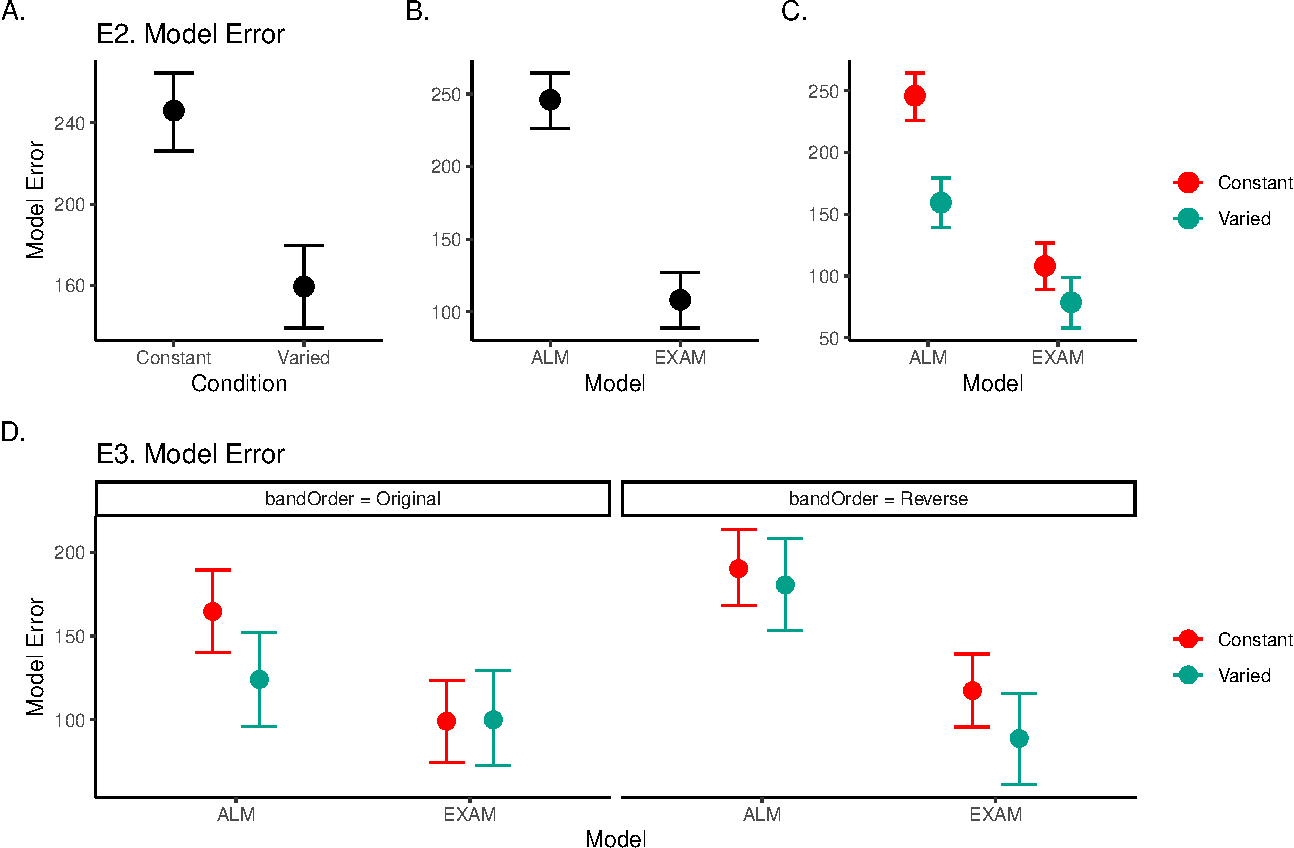
\includegraphics[keepaspectratio]{manuscript_files/figure-pdf/fig-e2_e3_ae-1.pdf}}

}

\caption{\label{fig-e2_e3_ae}Conditional effects of Model (ALM vs EXAM)
and Condition (Constant vs.~Varied) on Model Error for Experiments 2 and
3 data. Experiment 3 also includes a condition for the order of training
vs.~testing bands (original order vs.~reverse order).}

\end{figure}%

\emph{Computational Model Summary}. Across all three experiments, the
model fits consistently favored the Extrapolation-Association Model
(EXAM) over the Associative Learning Model (ALM). This preference for
EXAM was particularly pronounced for participants in the constant
training conditions (note the positive coefficients on
ModelEXAM:conditVaried interaction terms Table~\ref{tbl-htw-ee-e23}).
This pattern is clearly illustrated in Figure~\ref{fig-htw-best-model},
which plots the difference in model errors between ALM and EXAM for each
individual participant. Both varied and constant conditions have a
greater proportion of subjects better fit by EXAM (positive error
differences), with the magnitude of EXAM's advantage visibly larger for
the constant group.

The superior performance of EXAM, especially for the constant training
groups, may initially seem counterintuitive. One might assume that
exposure to multiple, varied examples would be necessary to extract an
abstract rule. However, EXAM is not a conventional rule-based model; it
does not require the explicit abstraction of a rule. Instead, rule-based
responses emerge during the retrieval process. The constant groups'
formation of a single, accurate input-output association, combined with
the usefulness of the zero point, seem to have been sufficient for EXAM
to capture their performance. A potential concern is that the assumption
of participants utilizing the zero point essentially transforms the
extrapolation problem into an interpolation problem. However, this
concern is mitigated by the consistency of the results across both the
original and reversed order conditions (the testing extrapolation bands
fall in between the constant training band and the 0 point in experiment
1, but not in experiment 2).

The fits to the individual participants also reveal a number of
interesting cases where the models struggle to capture the data
(Figure~\ref{fig-htw-indv-pred}). For example participant 68 exhibits a
strong non-monotonicity in the highest velocity band, a pattern which
ALM can mimic, but which EXAM cannot capture, given that it enforces a
simple linear relationship between target velocity and response.
Participant 70 (lower right corner of Figure~\ref{fig-htw-indv-pred})
had a roughly parabolic response pattern in their observed data, a
pattern which neither model can properly reproduce, but which causes
EXAM to perform particularly poorly.

\emph{Modeling Limitations.} The present work compared models based on
their ability to predict the observed data, without employing
conventional model fit indices such as the Akaike Information Criterion
(AIC) or the Bayesian Information Criterion (BIC). These indices, which
penalize models based on their number of free parameters, would have
been of limited utility in the current case, as both ALM and EXAM have
two free parameters. However, despite having the same number of free
parameters, EXAM could still be considered the more complex model, as it
incorporates all the components of ALM plus an additional mechanism for
rule-based responding. A more comprehensive model comparison approach
might involve performing cross-validation with a held-out subset of the
data (\citeproc{ref-mezzadriHoldoutStrategySelecting2022}{Mezzadri et
al., 2022}) or penalizing models based on the range of patterns they can
produce (\citeproc{ref-domeGdistanceComparisonModel2023}{Dome \& Wills,
2023}), under the assumption that more constrained models are more
impressive when they do adequately fit a given pattern of results.

\newpage{}

\begin{figure}

\centering{

\pandocbounded{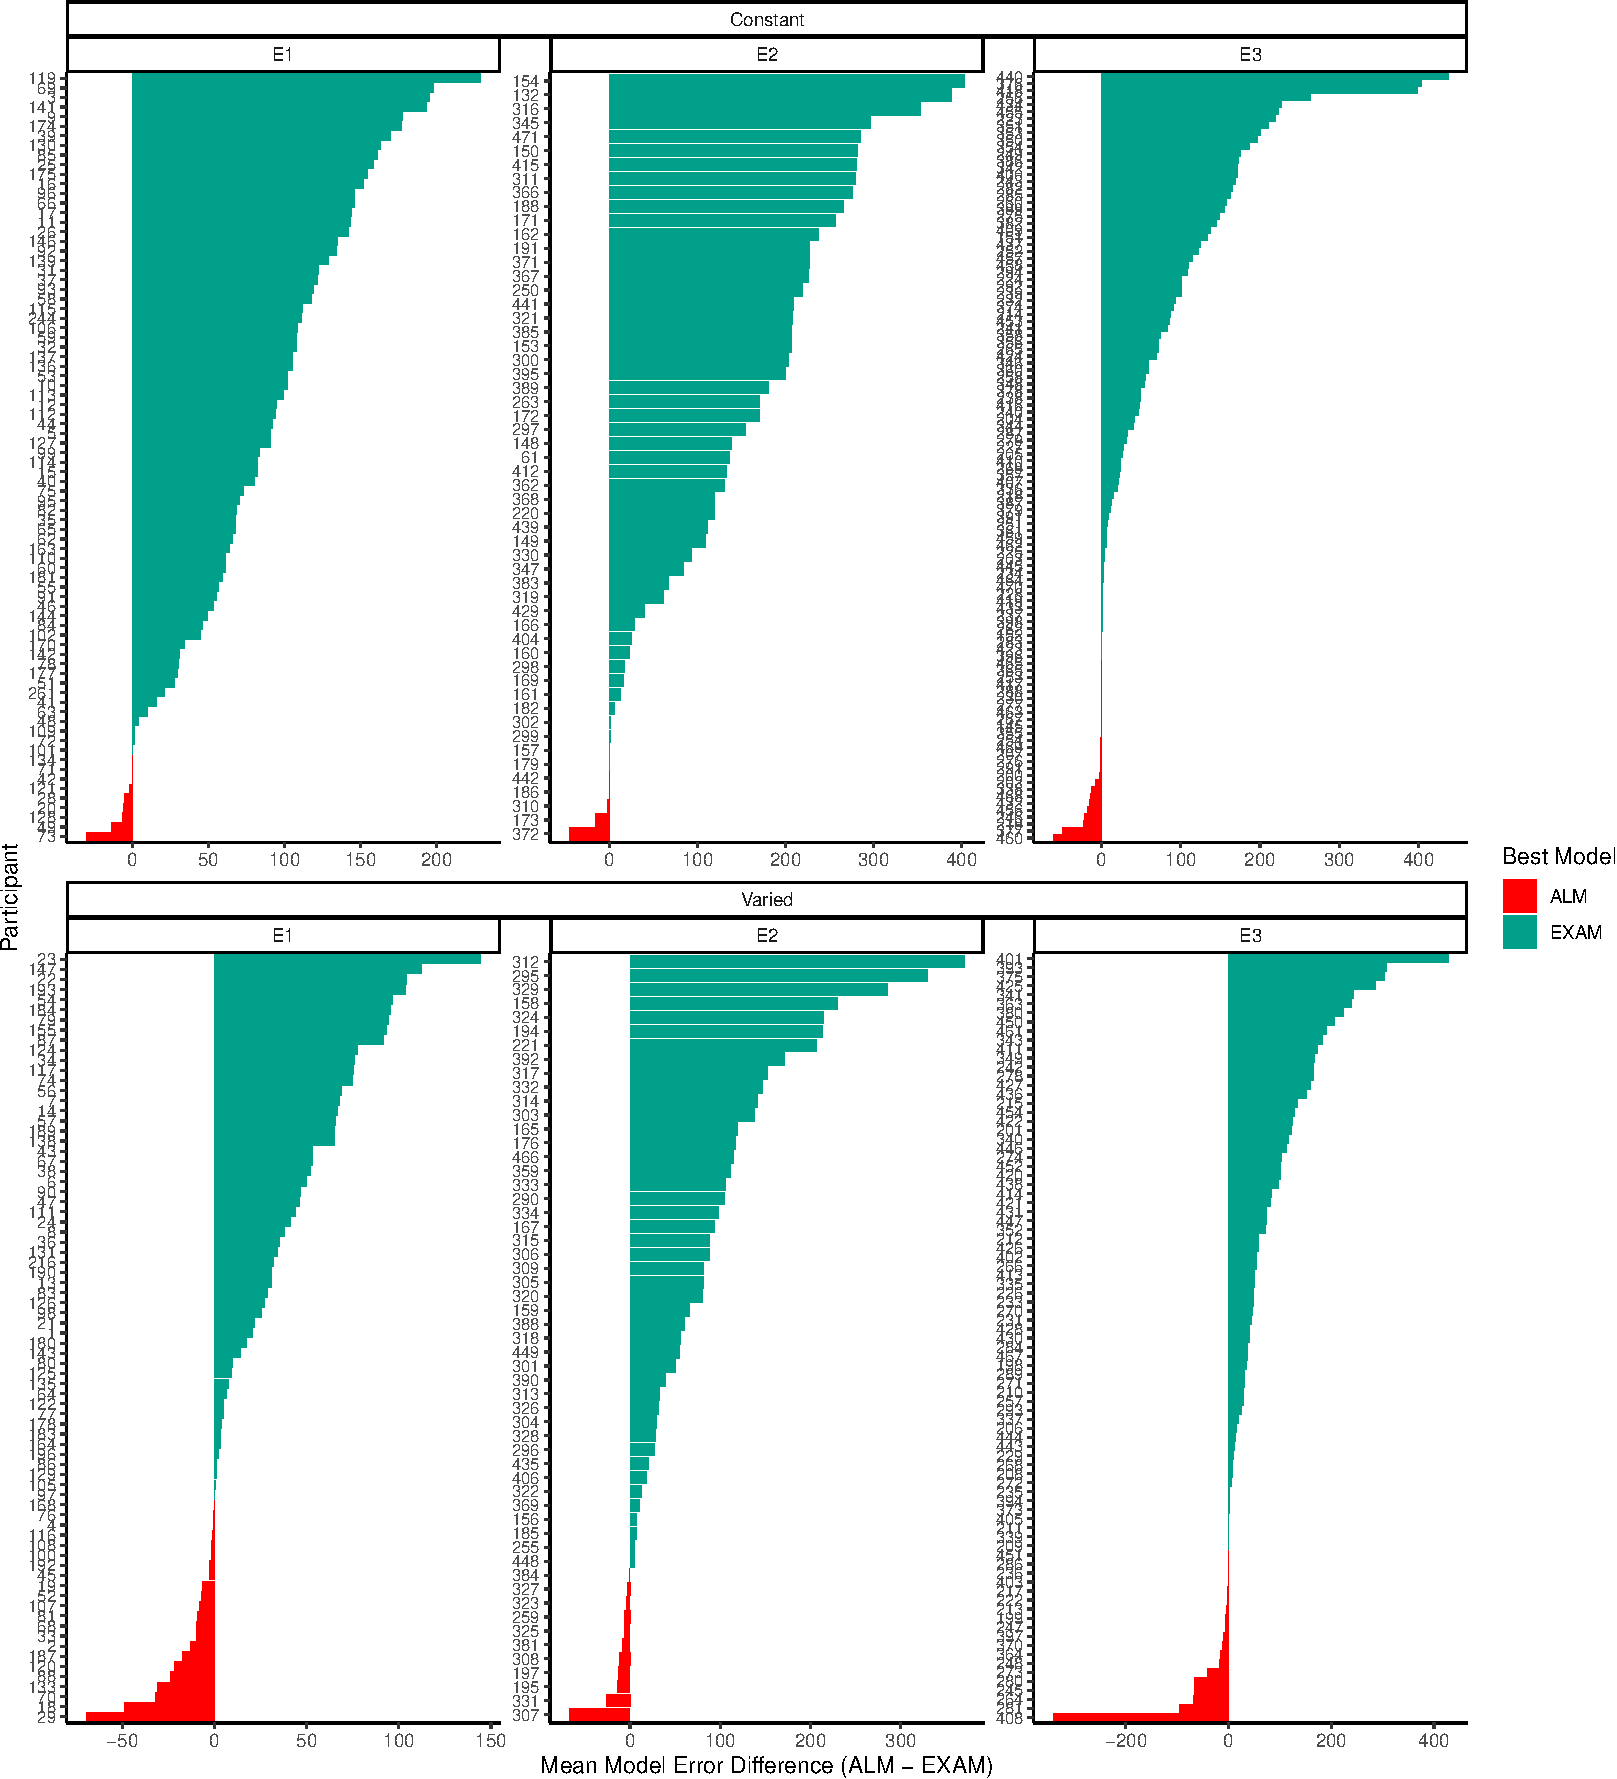
\includegraphics[keepaspectratio]{manuscript_files/figure-pdf/fig-htw-best-model-1.pdf}}

}

\caption{\label{fig-htw-best-model}Difference in model errors for each
participant, with models fit to both train and test data. Positive
values favor EXAM, while negative values favor ALM.}

\end{figure}%

\begin{figure}

\centering{

\pandocbounded{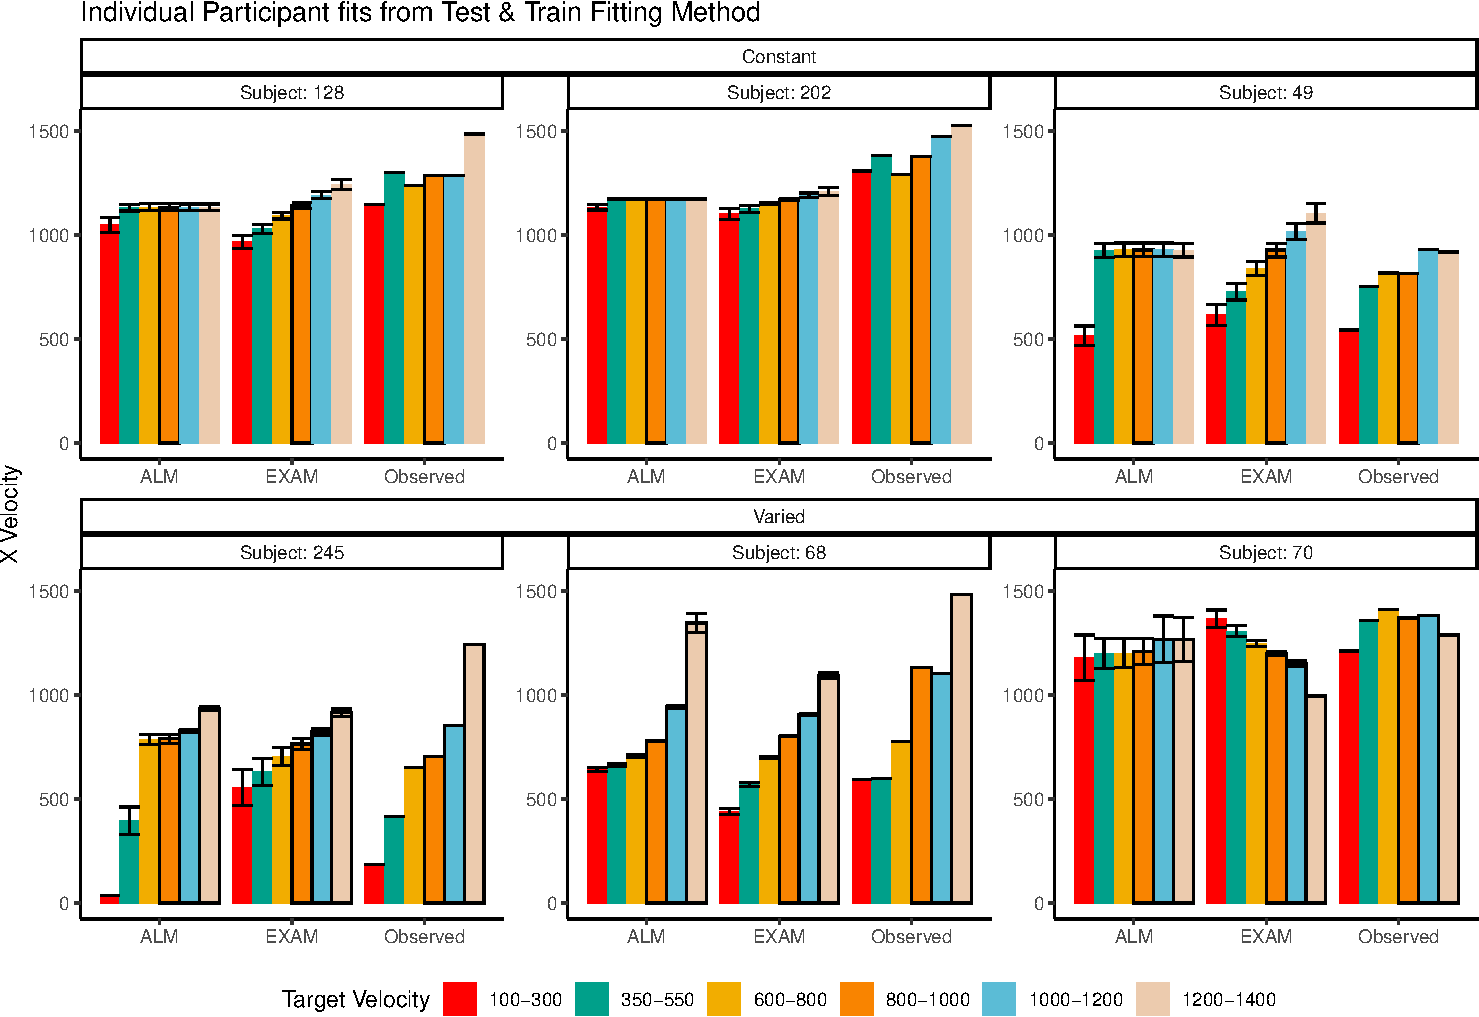
\includegraphics[keepaspectratio]{manuscript_files/figure-pdf/fig-htw-indv-pred-1.pdf}}

}

\caption{\label{fig-htw-indv-pred}Model predictions alongside observed
data for a subset of individual participants. A) 3 constant and 3 varied
participants fit to both the test and training data. B) 3 constant and 3
varied subjects fit to only the trainign data. Bolded bars indicate
bands that were trained, non-bold bars indicate extrapolation bands.}

\end{figure}%

\subsection{Project 2 Discussion}\label{project-2-discussion}

Across three experiments, we investigated the impact of training
variability on learning and extrapolation in a visuomotor function
learning task.

In Experiment 1, participants in the varied training condition, who
experienced a wider range of velocity bands during training, showed
lower accuracy at the end of training compared to those in the constant
training condition. Crucially, during the testing phase, the varied
group exhibited significantly larger deviations from the target velocity
bands, particularly for the extrapolation bands that were not
encountered during training. The varied group also showed less
discrimination between velocity bands, as evidenced by shallower slopes
when predicting response velocity from target velocity band.

Experiment 2 extended these findings by reversing the order of the
training and testing bands. Similar to Experiment 1, the varied group
demonstrated poorer performance during both training and testing phases.
However, unlike Experiment 1, the varied group did not show a
significant difference in discrimination between bands compared to the
constant group.

In Experiment 3, we provided only ordinal feedback during training, in
contrast to the continuous feedback provided in the previous
experiments. Participants were assigned to both an order condition
(original or reverse) and a training condition (constant or varied). The
varied condition showed larger deviations at the end of training,
consistent with the previous experiments. Interestingly, there was a
significant interaction between training condition and band order, with
the varied condition showing greater accuracy in the reverse order
condition. During testing, the varied group once again exhibited larger
deviations, particularly for the extrapolation bands. The reverse order
conditions showed smaller deviations compared to the original order
conditions. Discrimination between velocity bands was poorer for the
varied group in the original order condition, but not in the reverse
order condition.

All three of our experiments yielded evidence that varied training
conditions produced less learning by the end of training, a pattern
consistent with much of the previous research on the influence of
training variability
(\citeproc{ref-catalanoDistantTransferCoincident1984a}{Catalano \&
Kleiner, 1984};
\citeproc{ref-soderstromLearningPerformanceIntegrative2015}{Soderstrom
\& Bjork, 2015};
\citeproc{ref-wrisbergVariabilityPracticeHypothesis1987}{Wrisberg et
al., 1987}). The sole exception to this pattern was the reverse order
condition in Experiment 3, where the varied group was not significantly
worse than the constant group. Neither the varied condition trained with
the same reverse-order items in Experiment 2, nor the original-order
varied condition trained with ordinal feedback in Experiment 3 were able
to match the performance of their complementary constant groups by the
end of training, suggesting that the relative success of the
ordinal-reverse ordered varied group cannot be attributed to item or
feedback effects alone.

Our findings also diverge from the two previous studies that cleanly
manipulated the variability of training items in a function learning
task (\citeproc{ref-deloshExtrapolationSineQua1997}{DeLosh et al.,
1997}; \citeproc{ref-vandamMappingShapeVisuomotor2015}{van Dam \& Ernst,
2015}), although the varied training condition of van Dam \& Ernst
(\citeproc{ref-vandamMappingShapeVisuomotor2015}{2015}) also exhibited
less learning, neither of these previous studies observed any difference
between training conditions in extrapolation to novel items. Like DeLosh
et al. (\citeproc{ref-deloshExtrapolationSineQua1997}{1997}), our
participants exhibited above chance extrapolation/discrimination of
novel items, however they observed no difference between any of their
three training conditions. A noteworthy difference between our studies
is that DeLosh et al.
(\citeproc{ref-deloshExtrapolationSineQua1997}{1997}) trained
participants with either 8, 20, or 50 unique items (all receiving the
same total number of training trials). These larger sets of unique
items, combined with the fact that participants achieved near ceiling
level performance by the end of training, may have made it more
difficult to observe any between-group differences of training variation
in their study. van Dam \& Ernst
(\citeproc{ref-vandamMappingShapeVisuomotor2015}{2015}) 's variability
manipulation was more similar to our own, as they trained participants
with either 2 or 5 unique items. However, although the mapping between
their input stimuli and motor responses was technically linear, the
input dimension was more complex than our own, as it was defined by the
degree of ``spikiness'' of the input shape. This entirely arbitrary
mapping also would have precluded any sensible ``0'' point, which may
partially explain why neither of their training conditions were able to
extrapolate linearly in the manner observed in the current study or in
DeLosh et al. (\citeproc{ref-deloshExtrapolationSineQua1997}{1997}).

To explain our results, we turned to the well established EXAM and ALM
models. The disproportionate success of EXAM in capturing the
performance of participants under the constant training condition
suggests that rule-based extrapolation can emerge even from a limited
set of training examples. This success hinges on the assumption that
participants are able to leverage prior knowledge of the zero-point
reference (\citeproc{ref-brownUnderestimationLinearFunction2017}{Brown
\& Lacroix, 2017};
\citeproc{ref-kwantesWhyPeopleUnderestimate2006}{Kwantes \& Neal,
2006}). The zero-point reference, combined with accurate learning of the
single trained velocity band enabled EXAM to capture the extrapolation
patterns of the constant participants. However, it's important to
acknowledge that the ALM model provided a better fit for a subset of
participants in each of our three experiment, highlighting the presence
of substantial individual differences in generalization patterns.

This finding illustrates the importance of considering task structure
when evaluating the effects of training variability on generalization
and extrapolation. Some tasks, like the one in this study, may permit
the use of zero-point knowledge or other prior information, while others
may not. For example, a zero point may be less relevant in visuomotor
tasks with complex rotations
(\citeproc{ref-rollerVariablePracticeLenses2001}{Roller et al., 2001};
\citeproc{ref-vandamMappingShapeVisuomotor2015}{van Dam \& Ernst,
2015}), or in complex sports techniques
(\citeproc{ref-northEffectConsistentVaried2019}{North et al., 2019}).
Future research should systematically investigate how different task
structures interact with training variability to influence learning
outcomes and generalization abilities, taking into account factors such
as the availability of prior knowledge, the complexity of the task, and
the specific learning mechanisms involved. This approach could help
reconcile seemingly contradictory findings in the literature and provide
more nuanced guidelines for designing effective training protocols
across various domains.

\emph{Limitations}

While the present study provides valuable insights into the influence of
training variability on visuomotor function learning and extrapolation,
there are several limitations that should be flagged. First, although
the constant training group never had experience from a velocity band
closer to the extrapolation bands than the varied group, they always had
three times more trials with the nearest velocity band. Such a
difference may be an unavoidable consequence of a varied vs.~constant
design which matches the total number of training trials between the two
groups. However, in order to more carefully tease apart the influence of
variability from the influence of frequency/repetition effects, future
research could explore alternative designs that maintain the variability
manipulation while equating the amount of training on the nearest
examples across conditions, such as by increasing the total number of
trials for the varied group. Another limitation is that the testing
stage did not include any interpolation items, i.e.~the participants
were tested only from the training bands they experienced during
training, or from extrapolation bands. The absence of interpolation
testing makes it more difficult to distinguish between the effects of
training variability on extrapolation specifically, as opposed to
generalization more broadly. Of course, the nature of the constant
training condition makes interpolation testing impossible to implement,
however future studies might compare training regimes that each include
at least 2 distinct items, but still differ in the total amount of
variability experienced, which would then allow groups to be compared in
terms of both interpolation and extrapolation testing. Finally, the task
employed in the present study consisted of only a linear, positive
function. Previous work in human function learning has repeatedly shown
that such functions are among the easiest to learn, but that humans are
nonetheless capable of learning negative, non-linear, or discontinuous
functions
(\citeproc{ref-busemeyerLearningFunctionalRelations1997}{Busemeyer et
al., 1997}; \citeproc{ref-deloshExtrapolationSineQua1997}{DeLosh et al.,
1997}; \citeproc{ref-kalishLearningExtrapolatingPeriodic2013}{Kalish,
2013}; \citeproc{ref-mcdanielPredictingTransferPerformance2009}{McDaniel
et al., 2009}). It thus remains an open question as to whether the
influence of training variability might interact with various components
of the to-be-learned function.

\section{General Discussion}\label{general-discussion}

To facilitate ease of comparison between the two projects and their
respective tasks, we'll now refer to project 1 as Hit The Target (HTT)
and project 2 as Hit The Wall (HTW).

\subsection{Empirical and Modeling
Summary}\label{empirical-and-modeling-summary}

Across both projects, we investigated the influence of training
variability on learning and generalization in computerized visuomotor
skill learning, and function learning tasks. In project 1 (HTT),
experiments 1 and 2 demonstrated that varied training led to superior
testing performance compared to constant training. In Experiment 1, the
varied group even outperformed the constant group even when testing from
the constant groups trained position. In contrast, Project 2 (HTW) found
the opposite pattern - the varied training groups exhibited poorer
performance than the constant groups, both in terms of training
accuracy, accuracy in extrapolation testing, and, in a subset of the
experiments, the varied group showed a diminished ability to
discriminate between bands. This detrimental effect of variability was
observed across three experiments, with the exception of the reverse
order condition in Experiment 3, where the varied group was able to
match the constant group's performance.

Both projects also included computational modeling componenents. In
Project 1, the IGAS model was introduced as a means of addressing the
lack of control for similarity between training and testing conditions
common to previous work in the ``benefits of variability'' literature.
The IGAS model provides a theoretically motivated method of quantifying
the similarity between training experience and testing conditions. The
resulting similarity metric (i.e.~our 1c-similarity) is shown to be a
significant predictor of testing performance on its own, and when added
as a covariate to the statistical model used to compare the constant and
varied training groups. We then showed the group-level effect of
training variability on testing performance can be accounted for with
the additional assumption that training variability influences the
generalization gradient. The contribution of the IGAS model was thus
twofold:~ 1) providing a theoretically justifiable method of
quantifying/controlling for similarity between training and testing, and
2) demonstrating the viability of a flexible-similarity based
generalization account for the empirically observed benefit of
variability in our task. Although similar approaches have been employed
in other domains, both contributions are novel additions to the large
body of research assessing the effect of constant vs.~varied training
manipulations in visuomotor skill tasks.

Although theoretically motivated, the IGAS model of Project 1 is best
categorized as a descriptive measurement-model. Sufficient to account
for group differences, but lacking the machinery necessary to provide a
full process-level account of how the empirical quantities of interest
are generated. In contrast, Project 2 (HTW) implemented a more robust
computational modeling approach, implementing and comparing full process
models (ALM \& EXAM), capable of generating predictions for both the
learning and testing stages of the experiment. ALM and EXAM have been
used as models of function learning, cue judgement, and forecasting
behavior in numerous studies over the past 25 years
(\citeproc{ref-brownUnderestimationLinearFunction2017}{Brown \& Lacroix,
2017}; \citeproc{ref-deloshExtrapolationSineQua1997}{DeLosh et al.,
1997}; \citeproc{ref-kaneApplicationsBiasVariance2020}{Kane \& Broomell,
2020}; \citeproc{ref-kelleyComparisonModelsLearning2008}{H. Kelley \&
Busemeyer, 2008}; \citeproc{ref-kwantesItemOrderMatters2012}{Kwantes et
al., 2012};
\citeproc{ref-mcdanielPredictingTransferPerformance2009}{McDaniel et
al., 2009};
\citeproc{ref-vonhelversenLearningMultiplecueJudgment2010}{Von Helversen
\& Rieskamp, 2010}). The present work presents the first application of
these models to the study of training variability in a visuomotor
function learning task. We fit both models to individual participant
data, using a form of simulation-based Bayesian parameter estimation
that allowed us to generate and compare the full posterior predictive
distributions of each model. EXAM provided the best overall account of
the testing data, and the advantage of EXAM over ALM was significantly
greater for the constant group. Notably, EXAM captured the constant
groups' ability to extrapolate linearly to novel velocity bands, despite
receiving training from only a single input-output pair. This finding
suggests that EXAM's linear extrapolation mechanism, combined with the
assumption of prior knowledge about the origin point (0, 0), was
sufficient to account for the constant groups' accurate extrapolation
performance. Such findings may offer a preliminary suggestion that
experience with a more variable set of training examples may be
detrimental to performance in simple extrapolation tasks.

\subsection{Differences between the two
Projects}\label{differences-between-the-two-projects}

The HTT and HTW tasks differ across numerous dimensions that may be
relevant to the opposing patterns observed in the two projects (see
Table~\ref{tbl-task-diff} for a detailed comparison of the two tasks).

In HTT, the salient perceptual elements of the task (i.e.~the launching
box, target and barrier) are subject to variation (i.e.~different
distances between the launching box and target), and the spatial layout
of these perceptually variable elements are intrinsically linked to the
task objective of striking the target. Conversely, the perceptual task
elements in HTW are invariant across trials, and the task objective is
specified by the target velocity value specified as a numeral at the top
of the screen. If the benefits of training variation do arise from the
formation and flexible retrieval of distinct memory traces, then the
lack of perceptual salience between training instances in the HTW task
may have limited any potential benefits of variability. Future work
could investigate this possibility further employing a modified version
of the HTW task wherein the correct velocity value is indicated by some
perceptual feature of the task (e.g., the color of the wall, or size of
the ball), rather than displaying the target velocity numerically.

The HTT and HTW tasks also differed in terms of general task complexity.
The HTT task was designed to mimic projectile launching tasks commonly
employed in visuomotor learning studies, and the parabolic trajectories
necessary to strike the target in HTT were sensitive to both the x and y
dimensions of the projectiles velocity (and to a lesser extent, the
position within the launching box at which the ball was released).
Conversely the HTW task was influenced to a greater extent by the tasks
commonly utilized in the function learning literature, wherein the
correct output responses are determined by a single input dimension.
In~HTW, the relationship between feedback and optimal behavioral
adjustment is also almost perfectly smooth, if participants produce a
throw that is 100 units too hard, they'll be told that they were 100
units away from the target band. Whereas in HTT, the presence of the
barrier in introduces irregularities in the task space. Even throws
close to the solution space might result in failure, creating a less
predictable learning environment.

\begin{longtable}[]{@{}
  >{\raggedright\arraybackslash}p{(\linewidth - 4\tabcolsep) * \real{0.1577}}
  >{\raggedright\arraybackslash}p{(\linewidth - 4\tabcolsep) * \real{0.4732}}
  >{\raggedright\arraybackslash}p{(\linewidth - 4\tabcolsep) * \real{0.3691}}@{}}
\caption{Comparison of the tasks in Project 1 (HTT) and Project 2
(HTW).}\label{tbl-task-diff}\tabularnewline
\toprule\noalign{}
\begin{minipage}[b]{\linewidth}\raggedright
Dimension
\end{minipage} & \begin{minipage}[b]{\linewidth}\raggedright
HTT (Project 1)
\end{minipage} & \begin{minipage}[b]{\linewidth}\raggedright
HTW (Project 2)
\end{minipage} \\
\midrule\noalign{}
\endfirsthead
\toprule\noalign{}
\begin{minipage}[b]{\linewidth}\raggedright
Dimension
\end{minipage} & \begin{minipage}[b]{\linewidth}\raggedright
HTT (Project 1)
\end{minipage} & \begin{minipage}[b]{\linewidth}\raggedright
HTW (Project 2)
\end{minipage} \\
\midrule\noalign{}
\endhead
\bottomrule\noalign{}
\endlastfoot
Task Description & Projectile launching to hit a target & Projectile
launching to hit wall at a specific velocity \\
Task Complexity & More complex parabolic trajectory, both x and y
velocities relevant to outcome & Simpler 1D mapping of force to outcome.
Only x velocity is relevant. \\
Task Space & More complex: xy velocity combinations closer to the
solution space may still result in worse feedback due to striking the
barrier. & Simpler: smooth, linear mapping between velocity and
feedback. \\
Perceptual salience of Varied Conditions & Varied conditions (\# of
throwing distances) are perceptually distinct, i.e.~salient differences
in distance between launching box and target. & Varied conditions (\# of
velocity bands) are less salient - only difference is the numeral
displayed on screen. \\
Testing Feedback & Testing always included feedback & Primary testing
stage had no feedback. \\
Potential for Learning during Testing & Limited potential for learning
during testing due to feedback. & Some potential for learning during
no-feedback testing by observing ball trajectory. \\
Training Experience & Varied group gets half as much experience on any
one position as the constant group. & Varied group gets 1/3 as much
experience on any one velocity band as the constant group. \\
Testing Structure & Random interleaving of trained/transfer testing
distances. & Blocked structure, separately testing trained vs
extrapolation testing bands. \\
\end{longtable}

It is important to note that while both projects utilize computational
models, direct comparisons are complicated by the distinct purposes and
structures of the models used in each project. The IGAS model of Project
1 serves as a descriptive measurement model, capturing the similarity
between training throws and testing conditions. In contrast, the ALM and
EXAM models of Project 2 are full process models, capable of generating
exact predictions for both learning and testing stages. The difference
is also reflected in the interpretion of the generalization parameter
(\(c\)) across the models of the two projects. In IGAS, \(c\) moderates
the similarity between executed throws and subsequent testing solutions,
while in ALM and EXAM, \(c\) governs the extent to which the perceived
stimuli activate the input layer nodes. Despite these differences,
insights from ALM/EXAM, particularly the role of zero-point knowledge,
may offer potential explanations for the contrasting empirical results.
Particularly, EXAM's reliance on zero-point knowledge in the simpler HTW
task may explain why constant training was more effective in Project 2,
while the lack of a clear zero-point reference in the more complex HTT
task of Project 1 may have increased the value of varied training. This
suggests that the benefits of variability depend critically on how task
structure interacts with prior knowledge and the learner's capacity to
leverage such knowledge for generalization.

Future work could explore extending ALM and EXAM, which have
traditionally been applied to one-dimensional function learning tasks,
to more complex motor tasks such as HTT. The neural network structure of
ALM could be adapted to handle 2D input by utilizing a 2D grid of input
nodes, allowing the model to learn mappings between 2D throwing
velocities and desired outcomes. This would allow the model to process
the more complex spatial information inherent in tasks like HTT.
Furthermore, the output layers of ALM/EXAM could be expanded to express
more complex motor outputs in addition to velocity, such as the
locations of grabbing and releasing the projectile or other parameters
defining the unique trajectories produced. In addition to allowing the
models to be applied to more complex tasks, these modifications could
enable researchers to investigate how perceptual similarity (i.e., the
similarity of stimuli) and motoric similarity (i.e., the similarity of
behavioral actions) may separately and jointly influence learning and
generalization.

\subsection{Conclusion}\label{conclusion-1}

In summary, this dissertation provides a comprehensive examination of
the effects of training variability on learning and generalization in
visuomotor and function learning tasks. The contrasting results obtained
from the Hit The Target (HTT) and Hit The Wall (HTW) tasks underscore
the complexity inherent to the longstanding pedagogical and scientific
goal of identifying training manipulations that consistently benefit
learning and generalization. Moreover, through the development and
application of computational models, we provide novel theoretical
accounts for both the beneficial and detrimental effects of training
variability observed in our experiments. These findings highlight the
importance of considering task characteristics when designing
experiments intended to assess the influence of training interventions,
and demonstrate the value of combining empirical and computational
modeling approaches to uncover the cognitive mechanisms that support
learning and generalization. Future research should continue to
investigate the complex interplay between task demands, training
manipulations, and individual differences, with the goal of optimizing
educational and training outcomes across a wide range of domains.

~\\

\section{Appendix}\label{appendix}

\href{https://tegorman13.github.io/Dissertation/Sections/Appendix/Full_Appendix.html}{Apppendix}
available at
https://tegorman13.github.io/Dissertation/Sections/Appendix/Full\_Appendix.html

\section{References}\label{references}

\phantomsection\label{refs}
\begin{CSLReferences}{1}{0}
\bibitem[\citeproctext]{ref-ahaConceptLearningFlexible1992}
Aha, D. W., \& Goldstone, R. L. (1992). Concept {Learning} and {Flexible
Weighting}. \emph{In {Proceedings} of the {Fourteenth Annual Conference}
of the {Cognitive Science Society}}, 534--539.

\bibitem[\citeproctext]{ref-bengtssonUnifyingFrameworkParallel2021}
Bengtsson, H. (2021). A {Unifying Framework} for {Parallel} and
{Distributed Processing} in {R} using {Futures}. \emph{The R Journal},
\emph{13}(2), 208. \url{https://doi.org/10.32614/RJ-2021-048}

\bibitem[\citeproctext]{ref-bernikerEffectsTrainingBreadth2014}
Berniker, M., Mirzaei, H., \& Kording, K. P. (2014). The effects of
training breadth on motor generalization. \emph{Journal of
Neurophysiology}, \emph{112}(11), 2791--2798.
\url{https://doi.org/10.1152/jn.00615.2013}

\bibitem[\citeproctext]{ref-bjorkMakingThingsHard2011}
Bjork, E. L., \& Bjork, R. A. (2011). Making things hard on yourself,
but in a good way: {Creating} desirable difficulties to enhance
learning. \emph{Psychology and the Real World: Essays Illustrating
Fundamental Contributions to Society}, \emph{2}, 59--68.

\bibitem[\citeproctext]{ref-bottNonmonotonicExtrapolationFunction2004}
Bott, L., \& Heit, E. (2004). Nonmonotonic {Extrapolation} in {Function
Learning}. \emph{Journal of Experimental Psychology: Learning, Memory,
and Cognition}, \emph{30}(1), 38--50.
\url{https://doi.org/10.1037/0278-7393.30.1.38}

\bibitem[\citeproctext]{ref-bowmanTrainingSetCoherence2020}
Bowman, C. R., \& Zeithamova, D. (2020). Training set coherence and set
size effects on concept generalization and recognition. \emph{Journal of
Experimental Psychology. Learning, Memory, and Cognition}, \emph{46}(8),
1442--1464. \url{https://doi.org/10.1037/xlm0000824}

\bibitem[\citeproctext]{ref-braithwaiteEffectsVariationPrior2015}
Braithwaite, D. W., \& Goldstone, R. L. (2015). Effects of {Variation}
and {Prior Knowledge} on {Abstract Concept Learning}. \emph{Cognition
and Instruction}, \emph{33}(3), 226--256.
\url{https://doi.org/10.1080/07370008.2015.1067215}

\bibitem[\citeproctext]{ref-braunMotorTaskVariation2009}
Braun, D. A., Aertsen, A., Wolpert, D. M., \& Mehring, C. (2009). Motor
{Task Variation Induces Structural Learning}. \emph{Current Biology},
\emph{19}(4), 352--357. \url{https://doi.org/10.1016/j.cub.2009.01.036}

\bibitem[\citeproctext]{ref-brehmerHypothesesRelationsScaled1974}
Brehmer, B. (1974). Hypotheses about relations between scaled variables
in the learning of probabilistic inference tasks. \emph{Organizational
Behavior and Human Performance}, \emph{11}(1), 1--27.
\url{https://doi.org/10.1016/0030-5073(74)90002-6}

\bibitem[\citeproctext]{ref-brekelmansDoesHighVariability2022}
Brekelmans, G., Lavan, N., Saito, H., Clayards, M., \& Wonnacott, E.
(2022). Does high variability training improve the learning of
non-native phoneme contrasts over low variability training? {A}
replication. \emph{Journal of Memory and Language}, \emph{126}, 104352.
\url{https://doi.org/10.1016/j.jml.2022.104352}

\bibitem[\citeproctext]{ref-breslinConstantVariablePractice2012}
Breslin, G., Hodges, N. J., Steenson, A., \& Williams, A. M. (2012).
Constant or variable practice: {Recreating} the especial skill effect.
\emph{Acta Psychologica}, \emph{140}(2), 154--157.
\url{https://doi.org/10.1016/j.actpsy.2012.04.002}

\bibitem[\citeproctext]{ref-briscoeConceptualComplexityBias2011}
Briscoe, E., \& Feldman, J. (2011). Conceptual complexity and the
bias/variance tradeoff. \emph{Cognition}, \emph{118}(1), 2--16.
\url{https://doi.org/10.1016/j.cognition.2010.10.004}

\bibitem[\citeproctext]{ref-brownUnderestimationLinearFunction2017}
Brown, M. A., \& Lacroix, G. (2017). Underestimation in linear function
learning: {Anchoring} to zero or x-y similarity? \emph{Canadian Journal
of Experimental Psychology/Revue Canadienne de Psychologie
Exp{é}rimentale}, \emph{71}(4), 274--282.
\url{https://doi.org/10.1037/cep0000129}

\bibitem[\citeproctext]{ref-brunsteinPreparingNoveltyDiverse2011}
Brunstein, A., \& Gonzalez, C. (2011). Preparing for novelty with
diverse training. \emph{Applied Cognitive Psychology}, \emph{25}(5),
682--691. \url{https://doi.org/10.1002/acp.1739}

\bibitem[\citeproctext]{ref-burknerBrmsPackageBayesian2017}
Bürkner, P.-C. (2017). Brms: {An R Package} for {Bayesian Multilevel
Models Using Stan}. \emph{Journal of Statistical Software}, \emph{80},
1--28. \url{https://doi.org/10.18637/jss.v080.i01}

\bibitem[\citeproctext]{ref-burtonIdentityVariationRepresentations2016}
Burton, A. M., Kramer, R. S. S., Ritchie, K. L., \& Jenkins, R. (2016).
Identity {From Variation}: {Representations} of {Faces Derived From
Multiple Instances}. \emph{Cognitive Science}, \emph{40}(1), 202--223.
\url{https://doi.org/10.1111/cogs.12231}

\bibitem[\citeproctext]{ref-busemeyerLearningFunctionalRelations1997}
Busemeyer, J. R., Byun, E., DeLosh, E. L., \& McDaniel, M. A. (1997).
Learning {Functional Relations Based} on {Experience} with {Input-output
Pairs} by {Humans} and {Artificial Neural Networks}. In \emph{Knowledge
{Concepts} and {Categories}} (pp. 405--437). Psychology Press.

\bibitem[\citeproctext]{ref-carrollFunctionalLearningLearning1963}
Carroll, J. D. (1963). Functional {Learning}: {The Learning} of
{Continuous Functional Mappings Relating Stimulus} and {Response
Continua}. \emph{ETS Research Bulletin Series}, \emph{1963}(2), i--144.
\url{https://doi.org/10.1002/j.2333-8504.1963.tb00958.x}

\bibitem[\citeproctext]{ref-catalanoDistantTransferCoincident1984a}
Catalano, J. F., \& Kleiner, B. M. (1984). Distant {Transfer} in
{Coincident Timing} as a {Function} of {Variability} of {Practice}.
\emph{Perceptual and Motor Skills}, \emph{58}(3), 851--856.
\url{https://doi.org/10.2466/pms.1984.58.3.851}

\bibitem[\citeproctext]{ref-censorCommonMechanismsHuman2012}
Censor, N., Sagi, D., \& Cohen, L. G. (2012). Common mechanisms of human
perceptual and motor learning. \emph{Nature Reviews Neuroscience},
\emph{13}(9), 658--664. \url{https://doi.org/10.1038/nrn3315}

\bibitem[\citeproctext]{ref-chamberlinNoteSchemaExemplar1992}
Chamberlin, C. J., \& Magill, R. A. (1992a). A {Note} on {Schema} and
{Exemplar Approaches} to {Motor Skill Representation} in {Memory}.
\emph{Journal of Motor Behavior}, \emph{24}(2), 221--224.
\url{https://doi.org/10.1080/00222895.1992.9941617}

\bibitem[\citeproctext]{ref-chamberlinMemoryRepresentationMotor1992}
Chamberlin, C. J., \& Magill, R. A. (1992b). The {Memory Representation}
of {Motor Skills}: {A Test} of {Schema Theory}. \emph{Journal of Motor
Behavior}, \emph{24}(4), 309--319.
\url{https://doi.org/10.1080/00222895.1992.9941627}

\bibitem[\citeproctext]{ref-chuaPracticeVariabilityPromotes2019}
Chua, L.-K., Dimapilis, M. K., Iwatsuki, T., Abdollahipour, R.,
Lewthwaite, R., \& Wulf, G. (2019). Practice variability promotes an
external focus of attention and enhances motor skill learning.
\emph{Human Movement Science}, \emph{64}, 307--319.
\url{https://doi.org/10.1016/j.humov.2019.02.015}

\bibitem[\citeproctext]{ref-ciccioneCanHumansPerform2021}
Ciccione, L., \& Dehaene, S. (2021). Can humans perform mental
regression on a graph? {Accuracy} and bias in the perception of
scatterplots. \emph{Cognitive Psychology}, \emph{128}, 101406.
\url{https://doi.org/10.1016/j.cogpsych.2021.101406}

\bibitem[\citeproctext]{ref-cochraneTEfitsNonlinearRegression2020}
Cochrane, A. (2020). {TEfits}: {Nonlinear} regression for time-evolving
indices. \emph{Journal of Open Source Software}, \emph{5}(52), 2535.
\url{https://doi.org/10.21105/joss.02535}

\bibitem[\citeproctext]{ref-cohenCategoryVariabilityExemplar2001}
Cohen, A. L., Nosofsky, R. M., \& Zaki, S. R. (2001). Category
variability, exemplar similarity, and perceptual classification.
\emph{Memory \& Cognition}, \emph{29}(8), 1165--1175.
\url{https://doi.org/10.3758/BF03206386}

\bibitem[\citeproctext]{ref-cohenWhereGraspsAre2004}
Cohen, R. G., \& Rosenbaum, D. A. (2004). Where grasps are made reveals
how grasps are planned: Generation and recall of motor plans.
\emph{Experimental Brain Research}, \emph{157}(4).
\url{https://doi.org/10.1007/s00221-004-1862-9}

\bibitem[\citeproctext]{ref-cornwallEffectsCategoricalNumerical2022}
Cornwall, A. C., Davis, T., Byrne, K. A., \& Worthy, D. A. (2022).
Effects of categorical and numerical feedback on category learning.
\emph{Cognition}, \emph{225}, 105163.
\url{https://doi.org/10.1016/j.cognition.2022.105163}

\bibitem[\citeproctext]{ref-courrieuQuickApproximationBivariate2012}
Courrieu, P. (2012). Quick approximation of bivariate functions.
\emph{British Journal of Mathematical and Statistical Psychology},
\emph{65}(1), 89--121.
\url{https://doi.org/10.1111/j.2044-8317.2011.02016.x}

\bibitem[\citeproctext]{ref-cranmerFrontierSimulationbasedInference2020}
Cranmer, K., Brehmer, J., \& Louppe, G. (2020). The frontier of
simulation-based inference. \emph{Proceedings of the National Academy of
Sciences}, \emph{117}(48), 30055--30062.
\url{https://doi.org/10.1073/pnas.1912789117}

\bibitem[\citeproctext]{ref-crumpEpisodicContributionsSequential2010}
Crump, M. J. C., \& Logan, G. D. (2010). Episodic contributions to
sequential control: {Learning} from a typist's touch. \emph{Journal of
Experimental Psychology: Human Perception and Performance},
\emph{36}(3), 662--672. \url{https://doi.org/10.1037/a0018390}

\bibitem[\citeproctext]{ref-czyzVariabilityPracticeInformation2021}
Czyż, S. H. (2021). Variability of {Practice}, {Information Processing},
and {Decision Making}---{How Much Do We Know}? \emph{Frontiers in
Psychology}, \emph{12}. \url{https://doi.org/10.3389/fpsyg.2021.639131}

\bibitem[\citeproctext]{ref-deleeuwJsPsychJavaScriptLibrary2015}
de Leeuw, J. R. (2015). {jsPsych}: {A JavaScript} library for creating
behavioral experiments in a {Web} browser. \emph{Behavior Research
Methods}, \emph{47}(1), 1--12.
\url{https://doi.org/10.3758/s13428-014-0458-y}

\bibitem[\citeproctext]{ref-delreyEffectsContextualInterference1982}
Del Rey, P., Wughalter, E. H., \& Whitehurst, M. (1982). The {Effects}
of {Contextual Interference} on {Females With Varied Experience} in
{Open Sport Skills}. \emph{Research Quarterly for Exercise and Sport},
\emph{53}(2), 108--115.
\url{https://doi.org/10.1080/02701367.1982.10605236}

\bibitem[\citeproctext]{ref-deloshExtrapolationSineQua1997}
DeLosh, E. L., McDaniel, M. A., \& Busemeyer, J. R. (1997).
Extrapolation: {The Sine Qua Non} for {Abstraction} in {Function
Learning}. \emph{Journal of Experimental Psychology: Learning, Memory,
and Cognition}, \emph{23}(4), 19.
\url{https://doi.org/10.1037/0278-7393.23.4.968}

\bibitem[\citeproctext]{ref-domeGdistanceComparisonModel2023}
Dome, L., \& Wills, A. (2023). \emph{G-distance: {On} the comparison of
model and human heterogeneity} {[}Preprint{]}. PsyArXiv.
\url{https://doi.org/10.31234/osf.io/ygmcj}

\bibitem[\citeproctext]{ref-doyleMetacognitiveMonitoringCategory2016}
Doyle, M. E., \& Hourihan, K. L. (2016). Metacognitive monitoring during
category learning: How success affects future behaviour: {Memory}.
\emph{Memory}, \emph{24}(9), 1197--1207.
\url{https://doi.org/10.1080/09658211.2015.1086805}

\bibitem[\citeproctext]{ref-ennisMultidimensionalStochasticTheory1988}
Ennis, D. M., Palen, J. J., \& Mullen, K. (1988). A multidimensional
stochastic theory of similarity. \emph{Journal of Mathematical
Psychology}, \emph{32}(4), 449--465.
\url{https://doi.org/10.1016/0022-2496(88)90023-5}

\bibitem[\citeproctext]{ref-estesClassificationCognition1994}
Estes, W. K. (1994). \emph{Classification and {Cognition}}. Oxford
University Press.

\bibitem[\citeproctext]{ref-fanStimulusDiversityIncreases2022}
Fan, M., Zhang, D., Zhao, S., Xie, Q., Chen, W., Jie, J., Wang, Y., \&
Zheng, X. (2022). Stimulus diversity increases category-based fear
generalization and the effect of intolerance of uncertainty.
\emph{Behaviour Research and Therapy}, \emph{159}, 104201.
\url{https://doi.org/10.1016/j.brat.2022.104201}

\bibitem[\citeproctext]{ref-farrellComputationalModelingCognition2018}
Farrell, S., \& Lewandowsky, S. (2018). \emph{Computational {Modeling}
of {Cognition} and {Behavior}:} (1st ed.). Cambridge University Press.
\url{https://doi.org/10.1017/CBO9781316272503}

\bibitem[\citeproctext]{ref-faulStatisticalPowerAnalyses2009}
Faul, F., Erdfelder, E., Buchner, A., \& Lang, A.-G. (2009). Statistical
power analyses using {G}*{Power} 3.1: {Tests} for correlation and
regression analyses. \emph{Behavior Research Methods}, \emph{41}(4),
1149--1160. \url{https://doi.org/10.3758/BRM.41.4.1149}

\bibitem[\citeproctext]{ref-fulvioTaskSpecificResponseStrategy2014}
Fulvio, J. M., Green, C. S., \& Schrater, P. R. (2014). Task-{Specific
Response Strategy Selection} on the {Basis} of {Recent Training
Experience}. \emph{PLOS Computational Biology}, \emph{10}(1), e1003425.
\url{https://doi.org/10.1371/journal.pcbi.1003425}

\bibitem[\citeproctext]{ref-gandolfoMotorLearningField1996a}
Gandolfo, F., Mussa-Ivaldi, F. A., \& Bizzi, E. (1996). Motor learning
by field approximation. \emph{Proceedings of the National Academy of
Sciences}, \emph{93}(9), 3843--3846.
\url{https://doi.org/10.1073/pnas.93.9.3843}

\bibitem[\citeproctext]{ref-georgeStimulusVariabilityTask2021}
George, N., \& Egner, T. (2021). Stimulus variability and task relevance
modulate binding-learning. \emph{Attention, Perception, \&
Psychophysics}. \url{https://doi.org/10.3758/s13414-021-02338-6}

\bibitem[\citeproctext]{ref-gershmanStructureLearningPrinciples2023}
Gershman, S. J., \& Cikara, M. (2023). Structure learning principles of
stereotype change. \emph{Psychonomic Bulletin \& Review}, \emph{30}(4),
1273--1293. \url{https://doi.org/10.3758/s13423-023-02252-y}

\bibitem[\citeproctext]{ref-ghahramaniGeneralizationLocalRemappings1996}
Ghahramani, Z., Wolpert, D. M., \& Jordan, M. I. (1996). Generalization
to {Local Remappings} of the {Visuomotor Coordinate Transformation}.
\emph{Journal of Neuroscience}, \emph{16}(21), 7085--7096.
\url{https://doi.org/10.1523/JNEUROSCI.16-21-07085.1996}

\bibitem[\citeproctext]{ref-gonzalezDiversityTrainingEnhances2011}
Gonzalez, C., \& Madhavan, P. (2011). Diversity during training enhances
detection of novel stimuli. \emph{Journal of Cognitive Psychology},
\emph{23}(3), 342--350.
\url{https://doi.org/10.1080/20445911.2011.507187}

\bibitem[\citeproctext]{ref-goodeSuperiorityVariableRepeated2008}
Goode, M. K., Geraci, L., \& Roediger, H. L. (2008). Superiority of
variable to repeated practice in transfer on anagram solution.
\emph{Psychonomic Bulletin \& Review}, \emph{15}(3), 662--666.
\url{https://doi.org/10.3758/PBR.15.3.662}

\bibitem[\citeproctext]{ref-goodwinEffectDifferentQuantities1998}
Goodwin, J. E., Eckerson, J. M., Grimes, C. R., \& Gordon, P. M. (1998).
Effect of {Different Quantities} of {Variable Practice} on
{Acquisition}, {Retention}, and {Transfer} of {An Applied Motor Skill}.
\emph{Perceptual and Motor Skills}, \emph{87}(1), 147--151.
\url{https://doi.org/10.2466/pms.1998.87.1.147}

\bibitem[\citeproctext]{ref-gormanInstancebasedModelAccount2022}
Gorman, T. E., \& Goldstone, R. L. (2022). An instance-based model
account of the benefits of varied practice in visuomotor skill.
\emph{Cognitive Psychology}, \emph{137}, 101491.
\url{https://doi.org/10.1016/j.cogpsych.2022.101491}

\bibitem[\citeproctext]{ref-greenPracticeVariabilityTransfer1995a}
Green, D. P., Whitehead, J., \& Sugden, D. A. (1995). Practice
{Variability} and {Transfer} of a {Racket Skill}. \emph{Perceptual and
Motor Skills}, \emph{81}(3\_suppl), 1275--1281.
\url{https://doi.org/10.2466/pms.1995.81.3f.1275}

\bibitem[\citeproctext]{ref-guadagnoliRelationshipContextualInterference1999}
Guadagnoli, M. A., Holcomb, W. R., \& Weber, T. J. (1999). The
relationship between contextual interference effects and performer
expertise on the learning of a putting task. \emph{Journal of Human
Movement Studies}, \emph{37}(1), 19--36.

\bibitem[\citeproctext]{ref-guadagnoliChallengePointFramework2004}
Guadagnoli, M. A., \& Lee, T. D. (2004). Challenge {Point}: {A
Framework} for {Conceptualizing} the {Effects} of {Various Practice
Conditions} in {Motor Learning}. \emph{Journal of Motor Behavior},
\emph{36}(2), 212--224. \url{https://doi.org/10.3200/JMBR.36.2.212-224}

\bibitem[\citeproctext]{ref-guoEffectsExampleVariability2014}
Guo, J.-P., Yang, L.-Y., \& Ding, Y. (2014). Effects of example
variability and prior knowledge in how students learn to solve
equations. \emph{European Journal of Psychology of Education},
\emph{29}(1), 21--42. \url{https://www.jstor.org/stable/43551124}

\bibitem[\citeproctext]{ref-hacquesVisualControlClimbing2022}
Hacques, G., Dicks, M., Komar, J., \& Seifert, L. (2022). Visual control
during climbing: {Variability} in practice fosters a proactive gaze
pattern. \emph{PLOS ONE}, \emph{17}(6), e0269794.
\url{https://doi.org/10.1371/journal.pone.0269794}

\bibitem[\citeproctext]{ref-hahnEffectsCategoryDiversity2005}
Hahn, U., Bailey, T. M., \& Elvin, L. B. C. (2005). Effects of category
diversity on learning, memory, and generalization. \emph{Memory \&
Cognition}, \emph{33}(2), 289--302.
\url{https://doi.org/10.3758/BF03195318}

\bibitem[\citeproctext]{ref-hillsCentralExecutiveSearch2010}
Hills, T. T., Todd, P. M., \& Goldstone, R. L. (2010). The central
executive as a search process: {Priming} exploration and exploitation
across domains. \emph{Journal of Experimental Psychology: General},
\emph{139}(4), 590--609. \url{https://doi.org/10.1037/a0020666}

\bibitem[\citeproctext]{ref-hintzmanMINERVASimulationModel1984}
Hintzman, D. L. (1984). {MINERVA} 2: {A} simulation model of human
memory. \emph{Behavior Research Methods, Instruments, \& Computers},
\emph{16}(2), 96--101. \url{https://doi.org/10.3758/BF03202365}

\bibitem[\citeproctext]{ref-hintzmanSchemaAbstractionMultipletrace1986}
Hintzman, D. L. (1986). "{Schema} abstraction" in a multiple-trace
memory model. \emph{Psychological Review}, \emph{93}(4), 411.

\bibitem[\citeproctext]{ref-homaCategoryBreadthAbstraction1976}
Homa, D., \& Vosburgh, R. (1976). Category breadth and the abstraction
of prototypical information. \emph{Journal of Experimental Psychology:
Human Learning and Memory}, \emph{2}(3), 322--330.
\url{https://doi.org/10.1037/0278-7393.2.3.322}

\bibitem[\citeproctext]{ref-hommelEventFilesEvidence1998}
Hommel, B. (1998). Event {Files}: {Evidence} for {Automatic Integration}
of {Stimulus-Response Episodes}. \emph{Visual Cognition}, \emph{5}(1-2),
183--216. \url{https://doi.org/10.1080/713756773}

\bibitem[\citeproctext]{ref-honigPerceptualSimilarityModulates2022}
Honig, T., Shoham, A., \& Yovel, G. (2022). Perceptual similarity
modulates effects of learning from variability on face recognition.
\emph{Vision Research}, \emph{201}, 108128.
\url{https://doi.org/10.1016/j.visres.2022.108128}

\bibitem[\citeproctext]{ref-hoschPriorExperienceVariability2023}
Hosch, A.-K., Wirtz, P., \& von Helversen, B. (2023). Prior {Experience}
of {Variability Influences Generalization} of {Unspecified Categories}.
\emph{Quarterly Journal of Experimental Psychology (2006)},
17470218231210491. \url{https://doi.org/10.1177/17470218231210491}

\bibitem[\citeproctext]{ref-hsuEffectsGenerativeDiscriminative2010}
Hsu, A. S., \& Griffiths, T. L. (2010). Effects of generative and
discriminative learning on use of category variability. \emph{32nd
Annual Conference of the Cognitive Science Society}, 7.

\bibitem[\citeproctext]{ref-huHighvariabilityTrainingDoes2024}
Hu, M., \& Nosofsky, R. M. (2024). High-variability training does not
enhance generalization in the prototype-distortion paradigm.
\emph{Memory \& Cognition}, 1--16.
\url{https://doi.org/10.3758/s13421-023-01516-1}

\bibitem[\citeproctext]{ref-huetEducationAttentionExplanation2011}
Huet, M., Jacobs, D. M., Camachon, C., Missenard, O., Gray, R., \&
Montagne, G. (2011). The education of attention as explanation of
variability of practice effects: {Learning} the final approach phase in
a flight simulator. \emph{Journal of Experimental Psychology: Human
Perception and Performance}, \emph{37}(6), 1841--1854.
\url{https://doi.org/10.1037/a0024386}

\bibitem[\citeproctext]{ref-jamiesonInstanceTheoryDomaingeneral2022}
Jamieson, R. K., Johns, B. T., Vokey, J. R., \& Jones, M. N. (2022).
Instance theory as a domain-general framework for cognitive psychology.
\emph{Nature Reviews Psychology}, \emph{1}(3), 174--183.
\url{https://doi.org/10.1038/s44159-022-00025-3}

\bibitem[\citeproctext]{ref-jonesDensityDistinctivenessEarly2020}
Jones, S. D., \& Brandt, S. (2020). Density and {Distinctiveness} in
{Early Word Learning}: {Evidence From Neural Network Simulations}.
\emph{Cognitive Science}, \emph{44}(1), e12812.
\url{https://doi.org/10.1111/cogs.12812}

\bibitem[\citeproctext]{ref-kalishLearningExtrapolatingPeriodic2013}
Kalish, M. L. (2013). Learning and extrapolating a periodic function.
\emph{Memory \& Cognition}, \emph{41}(6), 886--896.
\url{https://doi.org/10.3758/s13421-013-0306-9}

\bibitem[\citeproctext]{ref-kalishPopulationLinearExperts2004}
Kalish, M. L., Lewandowsky, S., \& Kruschke, J. K. (2004). Population of
{Linear Experts}: {Knowledge Partitioning} and {Function Learning}.
\emph{Psychological Review}, \emph{111}(4), 1072--1099.
\url{https://doi.org/10.1037/0033-295X.111.4.1072}

\bibitem[\citeproctext]{ref-kaneApplicationsBiasVariance2020}
Kane, P. B., \& Broomell, S. B. (2020). Applications of the
bias--variance decomposition to human forecasting. \emph{Journal of
Mathematical Psychology}, \emph{98}, 102417.
\url{https://doi.org/10.1016/j.jmp.2020.102417}

\bibitem[\citeproctext]{ref-kangasraasioParameterInferenceComputational2019}
Kangasrääsiö, A., Jokinen, J. P. P., Oulasvirta, A., Howes, A., \&
Kaski, S. (2019). Parameter {Inference} for {Computational Cognitive
Models} with {Approximate Bayesian Computation}. \emph{Cognitive
Science}, \emph{43}(6), e12738. \url{https://doi.org/10.1111/cogs.12738}

\bibitem[\citeproctext]{ref-kassambaraRstatixPipeFriendlyFramework2021a}
Kassambara, A. (2021). \emph{Rstatix: {Pipe-Friendly Framework} for
{Basic Statistical Tests}}.

\bibitem[\citeproctext]{ref-kelleyComparisonModelsLearning2008}
Kelley, H., \& Busemeyer, J. (2008). A comparison of models for learning
how to dynamically integrate multiple cues in order to forecast
continuous criteria. \emph{Journal of Mathematical Psychology},
\emph{52}(4), 218--240. \url{https://doi.org/10.1016/j.jmp.2008.01.009}

\bibitem[\citeproctext]{ref-kelleyLearningAttendEffects2009}
Kelley, T. A., \& Yantis, S. (2009). Learning to attend: {Effects} of
practice on information selection. \emph{Journal of Vision},
\emph{9}(7), 16. \url{https://doi.org/10.1167/9.7.16}

\bibitem[\citeproctext]{ref-kerrSpecificVariedPractice1978}
Kerr, R., \& Booth, B. (1978). Specific and varied practice of motor
skill. \emph{Perceptual and Motor Skills}, \emph{46}(2), 395--401.
\url{https://doi.org/10.1177/003151257804600201}

\bibitem[\citeproctext]{ref-knappTheoryCategorizationBased1984}
Knapp, A. K., \& Anderson, J. A. (1984). Theory of categorization based
on distributed memory storage. \emph{Journal of Experimental Psychology:
Learning, Memory, and Cognition}, \emph{10}(4), 616--637.

\bibitem[\citeproctext]{ref-kohFunctionLearningInduction1991}
Koh, K., \& Meyer, D. E. (1991). Function learning: {Induction} of
continuous stimulus-response relations. \emph{Journal of Experimental
Psychology: Learning, Memory, and Cognition}, \emph{17}(5), 811.
\url{https://doi.org/10.1037/0278-7393.17.5.811}

\bibitem[\citeproctext]{ref-konovalovaInformationSamplingExplanation2020}
Konovalova, E., \& Le Mens, G. (2020). An information sampling
explanation for the in-group heterogeneity effect. \emph{Psychological
Review}, \emph{127}(1), 47--73. \url{https://doi.org/10.1037/rev0000160}

\bibitem[\citeproctext]{ref-kruschkeALCOVEExemplarbasedConnectionist1992}
Kruschke, J. K. (1992). {ALCOVE}: {An} exemplar-based connectionist
model of {Category Learning}. \emph{Psychological Review}, \emph{99}(1).
\url{https://doi.org/10.1037/0033-295X.99.1.22}

\bibitem[\citeproctext]{ref-kwantesWhyPeopleUnderestimate2006}
Kwantes, P. J., \& Neal, A. (2006). Why people underestimate y when
extrapolating in linear functions. \emph{Journal of Experimental
Psychology: Learning, Memory, and Cognition}, \emph{32}(5), 1019--1030.
\url{https://doi.org/10.1037/0278-7393.32.5.1019}

\bibitem[\citeproctext]{ref-kwantesItemOrderMatters2012}
Kwantes, P. J., Neal, A., \& Kalish, M. (2012). Item order matters in a
function learning task. \emph{Canadian Journal of Experimental
Psychology/Revue Canadienne de Psychologie Exp{é}rimentale},
\emph{66}(2), 90--97. \url{https://doi.org/10.1037/a0026639}

\bibitem[\citeproctext]{ref-lambertsFlexibleTuningSimilarity1994}
Lamberts, K. (1994). Flexible {Tuning} of {Similarity} in
{Exemplar-Based Categorization}. \emph{Journal of Experimental
Psychology: Learning, Memory, and Cognition}, \emph{20}(5), 1003--1021.
\url{https://doi.org/10.1037/0278-7393.20.5.1003}

\bibitem[\citeproctext]{ref-lavanEffectsHighVariability2019}
Lavan, N., Knight, S., Hazan, V., \& McGettigan, C. (2019). The effects
of high variability training on voice identity learning.
\emph{Cognition}, \emph{193}, 104026.
\url{https://doi.org/10.1016/j.cognition.2019.104026}

\bibitem[\citeproctext]{ref-lawSharedMechanismsPerceptual2010}
Law, C.-T., \& Gold, J. I. (2010). Shared {Mechanisms} of {Perceptual
Learning} and {Decision Making}. \emph{Topics in Cognitive Science},
\emph{2}(2), 226--238.
\url{https://doi.org/10.1111/j.1756-8765.2009.01044.x}

\bibitem[\citeproctext]{ref-leeEvidentialDiversityIncreases2019}
Lee, J. C., Lovibond, P. F., \& Hayes, B. K. (2019). Evidential
diversity increases generalisation in predictive learning.
\emph{Quarterly Journal of Experimental Psychology}, \emph{72}(11),
2647--2657. \url{https://doi.org/10.1177/1747021819857065}

\bibitem[\citeproctext]{ref-linvilleExemplarAbstractionModels1993}
Linville, P. W., \& Fischer, G. W. (1993). Exemplar and {Abstraction
Models} of {Perceived Group Variability} and {Stereotypicality}.
\emph{Social Cognition}, \emph{11}(1), 92--125.
\url{https://doi.org/10.1521/soco.1993.11.1.92}

\bibitem[\citeproctext]{ref-liveseyRevisitingPeakShift2019}
Livesey, E. J., \& McLaren, I. P. (2019). Revisiting peak shift on an
artificial dimension: {Effects} of stimulus variability on
generalisation. \emph{Quarterly Journal of Experimental Psychology},
\emph{72}(2), 132--150. \url{https://doi.org/10.1177/1747021817739832}

\bibitem[\citeproctext]{ref-loganInstanceTheoryAutomatization1988}
Logan, G. D. (1988). Toward an instance theory of automatization.
\emph{Psychological Review}, \emph{95}(4), 492--527.
\url{https://doi.org/10.1037/0033-295X.95.4.492}

\bibitem[\citeproctext]{ref-loganInstanceTheoryAttention2002a}
Logan, G. D. (2002). An instance theory of attention and memory.
\emph{Psychological Review}, \emph{109}(2), 376--400.
\url{https://doi.org/10.1037/0033-295X.109.2.376}

\bibitem[\citeproctext]{ref-lovibondStimulusDiscriminabilityInduction2020}
Lovibond, P. F., Lee, J. C., \& Hayes, B. K. (2020). Stimulus
discriminability and induction as independent components of
generalization. \emph{Journal of Experimental Psychology: Learning,
Memory, and Cognition}, \emph{46}(6), 1106--1120.
\url{https://doi.org/10.1037/xlm0000779}

\bibitem[\citeproctext]{ref-maddoxStimulusRangeDiscontinuity2011}
Maddox, W. T., \& Filoteo, J. V. (2011). Stimulus range and
discontinuity effects on information-integration category learning and
generalization. \emph{Attention, Perception, \& Psychophysics},
\emph{73}(4), 1279--1295.
\url{https://doi.org/10.3758/s13414-011-0101-2}

\bibitem[\citeproctext]{ref-makowskiBayestestRDescribingEffects2019}
Makowski, D., Ben-Shachar, M. S., \& Lüdecke, D. (2019). {bayestestR}:
{Describing Effects} and their {Uncertainty}, {Existence} and
{Significance} within the {Bayesian Framework}. \emph{Journal of Open
Source Software}, \emph{4}(40), 1541.
\url{https://doi.org/10.21105/joss.01541}

\bibitem[\citeproctext]{ref-manentiVariabilityTrainingUnlocks2023}
Manenti, G. L., Dizaji, A. S., \& Schwiedrzik, C. M. (2023). Variability
in training unlocks generalization in visual perceptual learning through
invariant representations. \emph{Current Biology}, \emph{33}(5),
817--826.e3. \url{https://doi.org/10.1016/j.cub.2023.01.011}

\bibitem[\citeproctext]{ref-marongelliAdvantageFlexibleNeuronal2013}
Marongelli, E., \& Thoroughman, K. (2013). The advantage of flexible
neuronal tunings in neural network models for motor learning.
\emph{Frontiers in Computational Neuroscience}, \emph{7}, 100.
\url{https://doi.org/10.3389/fncom.2013.00100}

\bibitem[\citeproctext]{ref-mcclellandDistributedMemoryRepresentation1985}
McClelland, J. L., \& Rumelhart, D. E. (1985). Distributed memory and
the representation of general and specific information. \emph{Journal of
Experimental Psychology: General}, \emph{114}, 159--188.

\bibitem[\citeproctext]{ref-mccrackenTestSchemaTheory1977}
McCracken, H. D., \& Stelmach, G. E. (1977). A {Test} of the {Schema
Theory} of {Discrete Motor Learning}. \emph{Journal of Motor Behavior},
\emph{9}(3), 193--201.
\url{https://doi.org/10.1080/00222895.1977.10735109}

\bibitem[\citeproctext]{ref-mcdanielConceptualBasisFunction2005}
McDaniel, M. A., \& Busemeyer, J. R. (2005). The conceptual basis of
function learning and extrapolation: {Comparison} of rule-based and
associative-based models. \emph{Psychonomic Bulletin \& Review},
\emph{12}(1), 24--42. \url{https://doi.org/10.3758/BF03196347}

\bibitem[\citeproctext]{ref-mcdanielPredictingTransferPerformance2009}
McDaniel, M. A., Dimperio, E., Jacqueline A. Griego, \& Busemeyer, J. R.
(2009). Predicting transfer performance: {A} comparison of competing
function learning models. \emph{Journal of Experimental Psychology.
Learning, Memory, and Cognition}, \emph{35}, 173--195.
\url{https://doi.org/10.1037/a0013982}

\bibitem[\citeproctext]{ref-mcdanielEffectsSpacedMassed2013}
McDaniel, M. A., Fadler, C. L., \& Pashler, H. (2013). Effects of spaced
versus massed training in function learning. \emph{Journal of
Experimental Psychology: Learning, Memory, and Cognition}, \emph{39}(5),
1417--1432. \url{https://doi.org/10.1037/a0032184}

\bibitem[\citeproctext]{ref-medinContextTheoryClassification1978}
Medin, D. L., \& Schaffer, M. M. (1978). Context {Theory} of
{Classification Learning}. \emph{Psychological Review}, \emph{85}(3),
207. \url{https://doi.org/10.1037/0033-295X.85.3.207}

\bibitem[\citeproctext]{ref-meighWhatMemoryRepresentation2018}
Meigh, K. M., Shaiman, S., Tompkins, C. A., Abbott, K. V., \&
Nokes-Malach, T. (2018). What memory representation is acquired during
nonword speech production learning? {The} influence of stimulus features
and training modality on nonword encoding. \emph{Cogent Psychology},
\emph{5}(1), 1493714.
\url{https://doi.org/10.1080/23311908.2018.1493714}

\bibitem[\citeproctext]{ref-menonVariationPhotosSame2015}
Menon, N., White, D., \& Kemp, R. I. (2015). Variation in {Photos} of
the {Same Face Drives Improvements} in {Identity Verification}.
\emph{Perception}, \emph{44}(11), 1332--1341.
\url{https://doi.org/10.1177/0301006615599902}

\bibitem[\citeproctext]{ref-mezzadriHoldoutStrategySelecting2022}
Mezzadri, G., Laloë, T., Mathy, F., \& Reynaud-Bouret, P. (2022).
Hold-out strategy for selecting learning models: {Application} to
categorization subjected to presentation orders. \emph{Journal of
Mathematical Psychology}, \emph{109}, 102691.
\url{https://doi.org/10.1016/j.jmp.2022.102691}

\bibitem[\citeproctext]{ref-morgensternOneshotCategorizationNovel2019}
Morgenstern, Y., Schmidt, F., \& Fleming, R. W. (2019). One-shot
categorization of novel object classes in humans. \emph{Vision
Research}, \emph{165}, 98--108.
\url{https://doi.org/10.1016/j.visres.2019.09.005}

\bibitem[\citeproctext]{ref-moshon-cohenStimulusVariabilityImproves2024}
Moshon-Cohen, T. E., Weinbach, N., \& Bitan, T. (2024). Stimulus
variability improves generalization following response inhibition
training. \emph{Psychological Research}, 1--17.
\url{https://doi.org/10.1007/s00426-023-01913-w}

\bibitem[\citeproctext]{ref-moxleySchemaVariabilityPractice1979}
Moxley, S. E. (1979). Schema: {The Variability} of {Practice
Hypothesis}. \emph{Journal of Motor Behavior}, \emph{11}(1), 65--70.
\url{https://doi.org/10.1080/00222895.1979.10735173}

\bibitem[\citeproctext]{ref-newellSchemaTheory19752003}
Newell, K. M. (2003). Schema {Theory} (1975): {Retrospectives} and
{Prospectives}. \emph{Research Quarterly for Exercise and Sport},
\emph{74}(4), 383--388.
\url{https://doi.org/10.1080/02701367.2003.10609108}

\bibitem[\citeproctext]{ref-newellVariabilityPracticeTransfer1976}
Newell, K. M., \& Shapiro, D. C. (1976). Variability of {Practice} and
{Transfer} of {Training}: {Some Evidence Toward} a {Schema View} of
{Motor Learning}. \emph{Journal of Motor Behavior}, \emph{8}(3),
233--243. \url{https://doi.org/10.1080/00222895.1976.10735077}

\bibitem[\citeproctext]{ref-northEffectConsistentVaried2019}
North, J. S., Bezodis, N. E., Murphy, C. P., Runswick, O. R., Pocock,
C., \& Roca, A. (2019). The effect of consistent and varied
follow-through practice schedules on learning a table tennis backhand.
\emph{Journal of Sports Sciences}, \emph{37}(6), 613--620.
\url{https://doi.org/10.1080/02640414.2018.1522683}

\bibitem[\citeproctext]{ref-nosofskyAttentionSimilarityIdentificationcategorization1986}
Nosofsky, R. M. (1986). Attention, similarity, and the
identification-categorization relationship. \emph{Journal of
Experimental Psychology: General}, \emph{115}(1), 39--57.
\url{https://doi.org/10.1037/0096-3445.115.1.39}

\bibitem[\citeproctext]{ref-nosofskySimilarityScalingCognitive1992}
Nosofsky, R. M. (1992). Similarity scaling and cognitive process models.
\emph{Annual Review of Psychology}, \emph{43}(1), 25--53.
\url{https://doi.org/10.1146/annurev.ps.43.020192.000325}

\bibitem[\citeproctext]{ref-nosofskyExemplarbasedAccountsMultiplesystem2000}
Nosofsky, R. M., \& Johansen, M. K. (2000). Exemplar-based accounts of
"multiple-system" phenomena in perceptual categorization.
\emph{Psychonomic Bulletin \& Review}, \emph{7}(3), 375--402.
\url{https://doi.org/10.1007/BF03543066}

\bibitem[\citeproctext]{ref-nosofskyInvestigationsExemplarBasedConnectionist1992}
Nosofsky, R. M., \& Kruschke, J. K. (1992). Investigations of an
{Exemplar-Based Connectionist Model} of {Category Learning}. In D. L.
Medin (Ed.), \emph{Psychology of {Learning} and {Motivation}} (Vol. 28,
pp. 207--250). Academic Press.
\url{https://doi.org/10.1016/S0079-7421(08)60491-0}

\bibitem[\citeproctext]{ref-nosofskyModelguidedSearchOptimal2019}
Nosofsky, R. M., Sanders, C. A., Zhu, X., \& McDaniel, M. A. (2019).
Model-guided search for optimal natural-science-category training
exemplars: {A} work in progress. \emph{Psychonomic Bulletin \& Review},
\emph{26}(1), 48--76. \url{https://doi.org/10.3758/s13423-018-1508-8}

\bibitem[\citeproctext]{ref-opdebeeckRepresentationPerceivedShape2008}
Op de Beeck, H. P., Wagemans, J., \& Vogels, R. (2008). The
representation of perceived shape similarity and its role for category
learning in monkeys: {A} modeling study. \emph{Vision Research},
\emph{48}(4), 598--610.
\url{https://doi.org/10.1016/j.visres.2007.11.019}

\bibitem[\citeproctext]{ref-pachecoLearningSpecificIndividual2018}
Pacheco, M. M., \& Newell, K. M. (2018). Learning a specific, individual
and generalizable coordination function: Evaluating the variability of
practice hypothesis in motor learning. \emph{Experimental Brain
Research}, \emph{236}(12), 3307--3318.
\url{https://doi.org/10.1007/s00221-018-5383-3}

\bibitem[\citeproctext]{ref-pageConnectionistModellingPsychology2000a}
Page, M. (2000). Connectionist modelling in psychology: {A} localist
manifesto. \emph{Behavioral and Brain Sciences}, \emph{23}(4), 443--467.
\url{https://doi.org/10.1017/S0140525X00003356}

\bibitem[\citeproctext]{ref-palmeriExemplarSimilarityDevelopment1997}
Palmeri, T. J. (1997). Exemplar {Similarity} and the {Development} of
{Automaticity}. \emph{Journal of Experimental Psychology: Human Learning
and Memory}, \emph{23}(2), 324--354.

\bibitem[\citeproctext]{ref-palmeriCentralTendenciesExtreme2001}
Palmeri, T. J., \& Nosofsky, R. M. (2001). Central {Tendencies},
{Extreme Points}, and {Prototype Enhancement Effects} in {Ill-Defined
Perceptual Categorization}. \emph{The Quarterly Journal of Experimental
Psychology Section A}, \emph{54}(1), 197--235.
\url{https://doi.org/10.1080/02724980042000084}

\bibitem[\citeproctext]{ref-parkPerceptionVariabilityCategory1987}
Park, B., \& Hastie, R. (1987). Perception of variability in category
development: {Instance-versus} abstraction-based stereotypes.
\emph{Journal of Personality and Social Psychology}, \emph{53}(4), 621.

\bibitem[\citeproctext]{ref-perlmanFurtherAttemptsClarify2012}
Perlman, A., Hahn, U., Edwards, D. J., \& Pothos, E. M. (2012). Further
attempts to clarify the importance of category variability for
categorisation. \emph{Journal of Cognitive Psychology}, \emph{24}(2),
203--220. \url{https://doi.org/10.1080/20445911.2011.613818}

\bibitem[\citeproctext]{ref-perryLearnLocallyThink2010}
Perry, L. K., Samuelson, L. K., Malloy, L. M., \& Schiffer, R. N.
(2010). Learn {Locally}, {Think Globally}: {Exemplar Variability
Supports Higher-Order Generalization} and {Word Learning}.
\emph{Psychological Science}, \emph{21}(12), 1894--1902.
\url{https://doi.org/10.1177/0956797610389189}

\bibitem[\citeproctext]{ref-pigottMotorSchemaStructure1984}
Pigott, R. E., \& Shapiro, D. C. (1984). Motor {Schema}: {The Structure}
of the {Variability Session}. \emph{Research Quarterly for Exercise and
Sport}, \emph{55}(1), 41--45.
\url{https://doi.org/10.1080/02701367.1984.10605353}

\bibitem[\citeproctext]{ref-plebanekEffectsFrequencyVariability2021}
Plebanek, D. J., \& James, K. H. (2021). The {Effects} of {Frequency},
{Variability}, and {Co-occurrence} on {Category Formation} in {Neural
Systems}. \emph{Journal of Cognitive Neuroscience}, 1--16.
\url{https://doi.org/10.1162/jocn_a_01738}

\bibitem[\citeproctext]{ref-poldrackRelationshipSkillLearning1999}
Poldrack, R. A., Selco, S. L., Field, J. E., \& Cohen, N. J. (1999). The
relationship between skill learning and repetition priming:
{Experimental} and computational analyses. \emph{Journal of Experimental
Psychology: Learning, Memory, and Cognition}, \emph{25}(1), 208--235.
\url{https://doi.org/10.1037/0278-7393.25.1.208}

\bibitem[\citeproctext]{ref-posnerGenesisAbstractIdeas1968}
Posner, M. I., \& Keele, S. W. (1968). On the genesis of abstract ideas.
\emph{Journal of Experimental Psychology}, \emph{77}(3), 353--363.
\url{https://doi.org/10.1037/h0025953}

\bibitem[\citeproctext]{ref-pradaExperiencedCategoryVariability2020}
Prada, M., \& Garcia-Marques, T. (2020). Experienced category
variability modulates the impact of context on evaluative judgments.
\emph{Experimental Psychology}, \emph{67}(1), 5--13.
\url{https://doi.org/10.1027/1618-3169/a000469}

\bibitem[\citeproctext]{ref-ramAnticipatedVariabilityIncreases2024}
Ram, H., Grinfeld, G., \& Liberman, N. (2024). Anticipated variability
increases generalization of predictive learning. \emph{Npj Science of
Learning}, \emph{9}(1), 1--10.
\url{https://doi.org/10.1038/s41539-024-00269-z}

\bibitem[\citeproctext]{ref-ravivHowVariabilityShapes2022}
Raviv, L., Lupyan, G., \& Green, S. C. (2022). How variability shapes
learning and generalization. \emph{Trends in Cognitive Sciences},
S1364661322000651. \url{https://doi.org/10.1016/j.tics.2022.03.007}

\bibitem[\citeproctext]{ref-reichmannVariabilityAbstractionEvaluative2023}
Reichmann, K., Hütter, M., Kaup, B., \& Ramscar, M. (2023). Variability
and abstraction in evaluative conditioning: {Consequences} for the
generalization of likes and dislikes. \emph{Journal of Experimental
Social Psychology}, \emph{108}, 104478.
\url{https://doi.org/10.1016/j.jesp.2023.104478}

\bibitem[\citeproctext]{ref-roarkComparingPerceptualCategory2021}
Roark, C. L., Paulon, G., Sarkar, A., \& Chandrasekaran, B. (2021).
Comparing perceptual category learning across modalities in the same
individuals. \emph{Psychonomic Bulletin \& Review}, \emph{28}(3),
898--909. \url{https://doi.org/10.3758/s13423-021-01878-0}

\bibitem[\citeproctext]{ref-robsonSpecificVariedPractice2022a}
Robson, S. G., Tangen, J. M., \& Searston, R. A. (2022). Specific versus
varied practice in perceptual expertise training. \emph{Journal of
Experimental Psychology: Human Perception and Performance},
\emph{48}(12), 1336--1346. \url{https://doi.org/10.1037/xhp0001057}

\bibitem[\citeproctext]{ref-rollerVariablePracticeLenses2001}
Roller, C. A., Cohen, H. S., Kimball, K. T., \& Bloomberg, J. J. (2001).
Variable practice with lenses improves visuo-motor plasticity.
\emph{Cognitive Brain Research}, \emph{12}(2), 341--352.
\url{https://doi.org/10.1016/S0926-6410(01)00077-5}

\bibitem[\citeproctext]{ref-rosenbaumAcquisitionIntellectualPerceptualMotor2001}
Rosenbaum, D. A., Carlson, R. A., \& Gilmore, R. O. (2001). Acquisition
of {Intellectual} and {Perceptual-Motor Skills}. \emph{Annual Review of
Psychology}, \emph{52}(1), 453--470.
\url{https://doi.org/10.1146/annurev.psych.52.1.453}

\bibitem[\citeproctext]{ref-rosenbaumPlanningReachesEvaluating1995}
Rosenbaum, D. A., Loukopoulos, L. D., Meulenbroek, R. G., Vaughan, J.,
\& Engelbrecht, S. E. (1995). Planning reaches by evaluating stored
postures. \emph{Psychological Review}, \emph{102}(1), 28.
\url{https://doi.org/10.1037/0033-295X.102.1.28}

\bibitem[\citeproctext]{ref-sabahWhenLessMore2019}
Sabah, K., Dolk, T., Meiran, N., \& Dreisbach, G. (2019). When less is
more: Costs and benefits of varied vs. Fixed content and structure in
short-term task switching training. \emph{Psychological Research},
\emph{83}(7), 1531--1542.
\url{https://doi.org/10.1007/s00426-018-1006-7}

\bibitem[\citeproctext]{ref-sadakataIndividualAptitudeMandarin2014}
Sadakata, M., \& McQueen, J. M. (2014). Individual aptitude in
{Mandarin} lexical tone perception predicts effectiveness of
high-variability training. \emph{Frontiers in Psychology}, \emph{5},
1318. \url{https://doi.org/10.3389/fpsyg.2014.01318}

\bibitem[\citeproctext]{ref-saidExtrapolationAccuracyUnderestimates2021}
Said, N., \& Fischer, H. (2021). Extrapolation accuracy underestimates
rule learning: {Evidence} from the function-learning paradigm.
\emph{Acta Psychologica}, \emph{218}, 103356.
\url{https://doi.org/10.1016/j.actpsy.2021.103356}

\bibitem[\citeproctext]{ref-sakamotoPuttingPsychologyBack2008}
Sakamoto, Y., Jones, M., \& Love, B. C. (2008). Putting the psychology
back into psychological models: {Mechanistic} versus rational
approaches. \emph{Memory \& Cognition}, \emph{36}(6), 1057--1065.
\url{https://doi.org/10.3758/MC.36.6.1057}

\bibitem[\citeproctext]{ref-sakamotoTrackingVariabilityLearning2006}
Sakamoto, Y., Love, B. C., \& Jones, M. (2006). Tracking {Variability}
in {Learning}: {Contrasting Statistical} and {Similarity-Based
Accounts}. \emph{Proceedings of the 28th Annual Conference of the
Cognitive Science Society. Vancouver, Canada: Cognitive Science
Society}.

\bibitem[\citeproctext]{ref-schmidtSchemaTheoryDiscrete1975}
Schmidt, R. A. (1975). A schema theory of discrete motor skill learning.
\emph{Psychological Review}, \emph{82}(4), 225--260.
\url{https://doi.org/10.1037/h0076770}

\bibitem[\citeproctext]{ref-schulzCommunicatingCompositionalPatterns2020}
Schulz, E., Quiroga, F., \& Gershman, S. J. (2020). Communicating
{Compositional Patterns}. \emph{Open Mind}, \emph{4}, 25--39.
\url{https://doi.org/10.1162/opmi_a_00032}

\bibitem[\citeproctext]{ref-seitzModelingCategoryVariability2023}
Seitz, F. I., Jarecki, J. B., \& Rieskamp, J. (2023). \emph{Modeling the
{Category Variability Effect} in an {Exemplar-Similarity Framework}}
{[}Preprint{]}. PsyArXiv.

\bibitem[\citeproctext]{ref-seowTransferEffectsVaried2019}
Seow, R. Y. T., Betts, S., \& Anderson, J. R. (2019). Transfer effects
of varied practice and adaptation to changes in complex skill
acquisition. \emph{Proceedings of the 17th International Conference on
Cognitive Modelling}, 222--227.

\bibitem[\citeproctext]{ref-shepardUniversalLawGeneralization1987}
Shepard, R. N. (1987). Toward a universal law of generalization for
psychological science. \emph{Science}, \emph{237}(4820), 1317--1323.
\url{https://doi.org/10.1126/science.3629243}

\bibitem[\citeproctext]{ref-sinkeviciuteRoleInputVariability2019}
Sinkeviciute, R., Brown, H., Brekelmans, G., \& Wonnacott, E. (2019).
The role of input variability and learner age in second language
vocabulary learning. \emph{Studies in Second Language Acquisition},
\emph{41}(04), 795--820. \url{https://doi.org/10.1017/S0272263119000263}

\bibitem[\citeproctext]{ref-soderstromLearningPerformanceIntegrative2015}
Soderstrom, N. C., \& Bjork, R. A. (2015). Learning versus performance:
{An} integrative review. \emph{Perspectives on Psychological Science},
\emph{10}(2), 176--199. \url{https://doi.org/10.1177/1745691615569000}

\bibitem[\citeproctext]{ref-stewartEffectCategoryVariability2002}
Stewart, N., \& Chater, N. (2002). The effect of category variability in
perceptual categorization. \emph{Journal of Experimental Psychology:
Learning, Memory, and Cognition}, \emph{28}(5), 893--907.
\url{https://doi.org/10.1037//0278-7393.28.5.893}

\bibitem[\citeproctext]{ref-taylorContextdependentGeneralization2013}
Taylor, J., \& Ivry, R. (2013). Context-dependent generalization.
\emph{Frontiers in Human Neuroscience}, \emph{7}, 171.
\url{https://doi.org/10.3389/fnhum.2013.00171}

\bibitem[\citeproctext]{ref-rcoreteamLanguageEnvironmentStatistical2020}
Team, R. C. (2020). \emph{R: {A Language} and {Environment} for
{Statistical Computing}}. R: A Language and Environment for Statistical
Computing.

\bibitem[\citeproctext]{ref-tenenbaumGeneralizationSimilarityBayesian2001a}
Tenenbaum, J. B., \& Griffiths, T. L. (2001). Generalization,
similarity, and {Bayesian} inference. \emph{Behavioral and Brain
Sciences}, \emph{24}(4), 629--640.
\url{https://doi.org/10.1017/S0140525X01000061}

\bibitem[\citeproctext]{ref-thoroughmanRapidReshapingHuman2005}
Thoroughman, K. A., \& Taylor, J. A. (2005). Rapid {Reshaping} of {Human
Motor Generalization}. \emph{Journal of Neuroscience}, \emph{25}(39),
8948--8953. \url{https://doi.org/10.1523/JNEUROSCI.1771-05.2005}

\bibitem[\citeproctext]{ref-turnerBayesianAnalysisSimulationbased2016}
Turner, B. M., Sederberg, P. B., \& McClelland, J. L. (2016). Bayesian
analysis of simulation-based models. \emph{Journal of Mathematical
Psychology}, \emph{72}, 191--199.
\url{https://doi.org/10.1016/j.jmp.2014.10.001}

\bibitem[\citeproctext]{ref-turnerTutorialApproximateBayesian2012}
Turner, B. M., \& Van Zandt, T. (2012). A tutorial on approximate
{Bayesian} computation. \emph{Journal of Mathematical Psychology},
\emph{56}(2), 69--85. \url{https://doi.org/10.1016/j.jmp.2012.02.005}

\bibitem[\citeproctext]{ref-twomeyAllRightNoises2018}
Twomey, K. E., Ma, L., \& Westermann, G. (2018). All the {Right Noises}:
{Background Variability Helps Early Word Learning}. \emph{Cognitive
Science}, \emph{42}(S2), 413--438.
\url{https://doi.org/10.1111/cogs.12539}

\bibitem[\citeproctext]{ref-vandamMappingShapeVisuomotor2015}
van Dam, L. C. J., \& Ernst, M. O. (2015). Mapping {Shape} to
{Visuomotor Mapping}: {Learning} and {Generalisation} of {Sensorimotor
Behaviour Based} on {Contextual Information}. \emph{PLOS Computational
Biology}, \emph{11}(3), e1004172.
\url{https://doi.org/10.1371/journal.pcbi.1004172}

\bibitem[\citeproctext]{ref-vanrossumSchmidtSchemaTheory1990}
Van Rossum, J. H. A. (1990). Schmidt's schema theory: The empirical base
of the variability of practice hypothesis. \emph{Human Movement
Science}, \emph{9}(3-5), 387--435.
\url{https://doi.org/10.1016/0167-9457(90)90010-B}

\bibitem[\citeproctext]{ref-velazquez-vargasRoleTrainingVariability2024}
Velázquez-Vargas, C. A., Daw, N. D., \& Taylor, J. A. (2024). The role
of training variability for model-based and model-free learning of an
arbitrary visuomotor mapping. \emph{PLOS Computational Biology},
\emph{20}(9), e1012471.
\url{https://doi.org/10.1371/journal.pcbi.1012471}

\bibitem[\citeproctext]{ref-vigoLearningDifficultyVisual2018}
Vigo, R., Doan, K.-M. C., Doan, C. A., \& Pinegar, S. (2018). On the
learning difficulty of visual and auditory modal concepts: {Evidence}
for a single processing system. \emph{Cognitive Processing},
\emph{19}(1), 1--16. \url{https://doi.org/10.1007/s10339-017-0840-7}

\bibitem[\citeproctext]{ref-vonhelversenLearningMultiplecueJudgment2010}
Von Helversen, B., \& Rieskamp, J. (2010). \emph{Learning in
multiple-cue judgment tasks}. \url{https://doi.org/10.5167/UZH-135898}

\bibitem[\citeproctext]{ref-wahlheimMetacognitiveJudgmentsRepetition2012}
Wahlheim, C. N., Finn, B., \& Jacoby, L. L. (2012). Metacognitive
judgments of repetition and variability effects in natural concept
learning: Evidence for variability neglect. \emph{Memory \& Cognition},
\emph{40}(5), 703--716. \url{https://doi.org/10.3758/s13421-011-0180-2}

\bibitem[\citeproctext]{ref-wallIdentifyingRelationshipsCognitive2021}
Wall, L., Gunawan, D., Brown, S. D., Tran, M.-N., Kohn, R., \& Hawkins,
G. E. (2021). Identifying relationships between cognitive processes
across tasks, contexts, and time. \emph{Behavior Research Methods},
\emph{53}(1), 78--95. \url{https://doi.org/10.3758/s13428-020-01405-4}

\bibitem[\citeproctext]{ref-wifallReachingResponseSelection2017}
Wifall, T., Buss, A. T., Farmer, T. A., Spencer, J. P., \& Hazeltine, E.
(2017). Reaching into response selection: {Stimulus} and response
similarity influence central operations. \emph{Journal of Experimental
Psychology: Human Perception and Performance}, \emph{43}(3), 555--568.
\url{https://doi.org/10.1037/xhp0000301}

\bibitem[\citeproctext]{ref-willeyLimitedGeneralizationVaried2018}
Willey, C. R., \& Liu, Z. (2018a). Limited generalization with varied,
as compared to specific, practice in short-term motor learning.
\emph{Acta Psychologica}, \emph{182}, 39--45.
\url{https://doi.org/10.1016/j.actpsy.2017.11.008}

\bibitem[\citeproctext]{ref-willeyLongtermMotorLearning2018}
Willey, C. R., \& Liu, Z. (2018b). Long-term motor learning: {Effects}
of varied and specific practice. \emph{Vision Research}, \emph{152},
10--16. \url{https://doi.org/10.1016/j.visres.2017.03.012}

\bibitem[\citeproctext]{ref-wonnacottInputEffectsAcquisition2012}
Wonnacott, E., Boyd, J. K., Thomson, J., \& Goldberg, A. E. (2012).
Input effects on the acquisition of a novel phrasal construction in
5year olds. \emph{Journal of Memory and Language}, \emph{66}(3),
458--478. \url{https://doi.org/10.1016/j.jml.2011.11.004}

\bibitem[\citeproctext]{ref-wrisbergTrainingProductionNovel1984}
Wrisberg, C. A., \& McLean, E. (1984). Training for the production of
novel timing movements: {Contextual} considerations. \emph{Psychological
Research}, \emph{46}(1-2), 169--176.
\url{https://doi.org/10.1007/BF00308601}

\bibitem[\citeproctext]{ref-wrisbergDevelopingCoincidentTiming1983}
Wrisberg, C. A., \& Mead, B. J. (1983). Developing {Coincident Timing
Skill} in {Children}: {A Comparison} of {Training Methods}.
\emph{Research Quarterly for Exercise and Sport}, \emph{54}(1), 67--74.
\url{https://doi.org/10.1080/02701367.1983.10605274}

\bibitem[\citeproctext]{ref-wrisbergVariabilityPracticeHypothesis1987}
Wrisberg, C. A., Winter, T. P., \& Kuhlman, J. S. (1987). The
{Variability} of {Practice Hypothesis}: {Further Tests} and
{Methodological Discussion}. \emph{Research Quarterly for Exercise and
Sport}, \emph{58}(4), 369--374.
\url{https://doi.org/10.1080/02701367.1987.10608114}

\bibitem[\citeproctext]{ref-wuSimilaritiesDifferencesSpatial2020}
Wu, C. M., Schulz, E., Garvert, M. M., Meder, B., \& Schuck, N. W.
(2020). Similarities and differences in spatial and non-spatial
cognitive maps. \emph{PLOS Computational Biology}, \emph{16}(9).
\url{https://doi.org/10.1101/2020.01.21.914556}

\bibitem[\citeproctext]{ref-wulfEffectTypePractice1991}
Wulf, G. (1991). The effect of type of practice on motor learning in
children. \emph{Applied Cognitive Psychology}, \emph{5}(2), 123--134.
\url{https://doi.org/10.1002/acp.2350050206}

\bibitem[\citeproctext]{ref-wulfVariabilityPracticeImplicit1997}
Wulf, G., \& Schmidt, R. A. (1997). \emph{Variability of {Practice} and
{Implicit Motor Learning}}.

\bibitem[\citeproctext]{ref-yangGeneralLearningAbility2020}
Yang, J., Yan, F.-F., Chen, L., Xi, J., Fan, S., Zhang, P., Lu, Z.-L.,
\& Huang, C.-B. (2020). General learning ability in perceptual learning.
\emph{Proceedings of the National Academy of Sciences}, \emph{117}(32),
19092--19100. \url{https://doi.org/10.1073/pnas.2002903117}

\bibitem[\citeproctext]{ref-yangCategoryVariabilityEffect2014}
Yang, L.-X., \& Wu, Y.-H. (2014). Category variability effect in
category learning with auditory stimuli. \emph{Frontiers in Psychology},
\emph{5}. \url{https://doi.org/10.3389/fpsyg.2014.01122}

\bibitem[\citeproctext]{ref-zakiHighdistortionEnhancementEffect2007}
Zaki, S. R., \& Nosofsky, R. M. (2007). A high-distortion enhancement
effect in the prototype-learning paradigm: {Dramatic} effects of
category learning during test. \emph{Memory \& Cognition}, \emph{35}(8),
2088--2096. \url{https://doi.org/10.3758/BF03192940}

\bibitem[\citeproctext]{ref-zamanPerceptualVariabilityImplications2021}
Zaman, J., Chalkia, A., Zenses, A.-K., Bilgin, A. S., Beckers, T.,
Vervliet, B., \& Boddez, Y. (2021). Perceptual variability:
{Implications} for learning and generalization. \emph{Psychonomic
Bulletin \& Review}, \emph{28}(1), 1--19.
\url{https://doi.org/10.3758/s13423-020-01780-1}

\bibitem[\citeproctext]{ref-zhangHighVariabilityLearning2024}
Zhang, T., \& Fyfe, E. R. (2024). High variability in learning materials
benefits children's pattern practice. \emph{Journal of Experimental
Child Psychology}, \emph{239}, 105829.
\url{https://doi.org/10.1016/j.jecp.2023.105829}

\end{CSLReferences}

\newpage{}

\pagenumbering{gobble}

\section{Curriculum Vitae}\label{curriculum-vitae}

\subsection*{Education}\label{education}

\begin{tabular}{p{0.3\textwidth} p{0.7\textwidth}}
2017 - May 2024 & \textbf{Indiana University - Bloomington} \\
& PhD in Psychology and Cognitive Science \\ 
& Dissertation: \textit{The Role of Variability in Learning Generalization: A Computational Modeling Approach}\\
2011 - 2015 & \textbf{University of Wisconsin - Madison} \\
& B.Sc. in Psychology \\
& Thesis: \textit{Short-term mindfulness intervention reduces the negative attentional effects associated with heavy media multitasking} \\
\end{tabular}

\subsection*{Journal Articles and Conference
Proceedings}\label{journal-articles-and-conference-proceedings}

\begin{itemize}
\item
  \textbf{Gorman}, T. E., \& Goldstone, R. L. (2022). An instance-based
  model account of the benefits of varied practice in visuomotor skill.
  \emph{Cognitive Psychology}, \emph{137}, 101491.
\item
  Kattner, F., Cochrane, A., Cox, C. R., \textbf{Gorman}, T. E., \&
  Green, C. S. (2017). Perceptual learning generalization from
  sequential perceptual training as a change in learning rate.
  \emph{Current Biology}, \emph{27}(6), 840-846.
\item
  \textbf{Gorman}, T.E., \& Green, C.S. (2016). Short-term mindfulness
  intervention reduces the negative attentional effects associated with
  heavy media multitasking. \emph{Scientific Reports}, \emph{6}.
\end{itemize}

\subsection*{Reviews and Book Chapters}\label{reviews-and-book-chapters}

\begin{itemize}
\item
  \textbf{Gorman}, T.E., Gentile, D.A., \& Green, C.S. Problem gaming: a
  short primer (2018). \emph{American Journal of Play}, \emph{10} (3),
  309-327
\item
  \textbf{Gorman}, T.E., \& Green, C.S. (2017). Young minds on video
  games. In \emph{Cognitive development in digital contexts}. 121-143.
  Academic Press.
\item
  Green, C. S., \textbf{Gorman}, T., \& Bavelier, D. (2016). Action
  Video-Game Training and Its Effects on Perception and Attentional
  Control. In \emph{Cognitive Training} (pp.~107-116). Springer
  International Publishing.
\end{itemize}

\subsection*{Presentations}\label{presentations}

\begin{itemize}
\tightlist
\item
  Half Day Tutorial on Measuring Mindfulness Behaviorally: Onsite/Online
  Data Col-lection with jsPsych - Cognitive Science Conference -- 2018
\item
  Does interleaving go the distance? Exploring the effect of
  dissimilarity on interleaved category learning - Math Psych/ICCM 2018
\item
  Short term mindfulness intervention reduces cognitive deficits in
  heavy media multi-taskers - Undergraduate Research Symposium --
  UW-Madison -- April 16th, 2015
\end{itemize}

\subsection*{Awards}\label{awards}

IU-Bloomington -- Development Training Grant -- Fall 2019

IU-Bloomington - Steinmetz Summer Research Award - 2018

UW-Madison - Undergraduate Research Scholar Award -- 2015

UW-Madison - Hilldale Undergraduate/Faculty Research Fellowship -- 2014

\subsection*{Ad-hoc Reviewer}\label{ad-hoc-reviewer}

Cognitive Science

Journal of Experimental Psychology: General

Journal of Experimental Psychology: Human Perception and Performance

\subsection*{Conferences}\label{conferences}

Cognitive Science Conference - 2021

Cognitive Science Conference - 2018

Mathematical Psychology \& ICCM 2018

Boston Meeting on Methods in Cognitive Training (NSF Sponsored) -- May
2017




\end{document}
